\documentclass{article}

% ── Page size — compatible with both pdfTeX and XeTeX ────────
\usepackage[letterpaper]{geometry}

% ── IJCAI two-column conference style ────────────────────────
\usepackage{ijcai26}
\usepackage{times}
\usepackage{soul}
\usepackage{url}
\usepackage[hidelinks]{hyperref}
\usepackage[utf8]{inputenc}
\usepackage[small]{caption}
\usepackage{graphicx}
\usepackage{amsmath}
\usepackage{amssymb}
\usepackage{amsthm}
\usepackage{booktabs}
\usepackage{multirow}
\usepackage{xcolor}
\usepackage{enumitem}
\usepackage{subcaption}
\usepackage{natbib}

% ── TikZ (diagrams) ─────────────────────────────────────────
\usepackage{tikz}
\usetikzlibrary{
  positioning, arrows.meta, shapes.geometric,
  shapes.multipart, fit, backgrounds,
  decorations.pathreplacing, decorations.markings,
  calc, patterns, matrix, chains, trees, shadows
}

% ── pgfplots (charts, experiment results) ────────────────────
\usepackage{pgfplots}
\pgfplotsset{compat=1.18}
\usepgfplotslibrary{groupplots, statistics}

% ── Algorithm typesetting ────────────────────────────────────
\usepackage{algorithm}
\usepackage{algorithmic}

% ── Code listings (YAML schemas, pipeline) ───────────────────
\usepackage{listings}
\lstset{
  basicstyle=\ttfamily\footnotesize,
  backgroundcolor=\color{black!3},
  frame=single, framerule=0.4pt,
  rulecolor=\color{black!20},
  breaklines=true, columns=fullflexible, keepspaces=true,
  captionpos=b, aboveskip=6pt, belowskip=6pt,
}

\urlstyle{same}

% ── Theorem-like environments ────────────────────────────────
\newtheorem{definition}{Definition}
\newtheorem{principle}{Design Principle}
\newtheorem{finding}{Finding}

% ── Shared TikZ styles ──────────────────────────────────────
\tikzset{
  sutra/agent/.style={draw, thick, circle, minimum size=10mm,
    font=\footnotesize\bfseries, inner sep=0pt},
  sutra/station/.style={draw, thick, rounded corners=4pt,
    minimum width=2.2cm, minimum height=1cm,
    font=\small, align=center, inner sep=4pt},
  sutra/classical/.style={draw, thick, rounded corners=3pt,
    fill=blue!8, minimum width=3cm, minimum height=0.8cm,
    font=\small, align=center},
  sutra/modern/.style={draw, thick, rounded corners=3pt,
    fill=green!8, minimum width=3cm, minimum height=0.8cm,
    font=\small, align=center},
  sutra/gap/.style={draw, thick, rounded corners=3pt,
    fill=red!8, minimum width=3cm, minimum height=0.8cm,
    font=\small, align=center},
  sutra/flow/.style={-{Stealth[length=5pt, width=4pt]}, thick},
  sutra/biflow/.style={{Stealth[length=4pt]}-{Stealth[length=4pt]}, thick},
  sutra/dashed/.style={-{Stealth[length=4pt]}, dashed, thin},
}


% ══════════════════════════════════════════════════════════════
\title{Sutra: Threading Classical Coordination\\
Through the Age of LLM Agents}

\author{
Balaji Viswanathan$^1$
\affiliations
$^1$Kapi AI\\
\emails
balaji@getkapi.com
}

\begin{document}
\maketitle

% ──────────────────────────────────────────────────────────────
% ABSTRACT
% ──────────────────────────────────────────────────────────────
\begin{abstract}
Multi-agent systems are experiencing a renaissance.  The frameworks
multiply monthly, a quarter of all MAS papers were published in the
last two years, and agentic AI has become a boardroom priority.  Yet
this renaissance carries a hidden cost.  The entire history of software
is built on a caller/callee paradigm---one entity commands, the other
obeys.  Multi-agent systems break this paradigm by introducing
\emph{peers}: entities that negotiate, refuse, bid, and pursue their
own goals.  That shift is fundamental, and the field that studied it for
thirty years---classical MAS research---is being largely ignored.
A fifteen-year quiet period between the classical era and the current
LLM-driven revival has created a generational gap: foundational
protocols like Contract Net, commitment tracking, and result sharing are
being independently reinvented without their formal guarantees, while
critical primitives like Functionally Accurate cooperation are missing
entirely.  We take the ambitious task of sifting through 36,000+ papers
in the field using a combination of human expertise and a 7-agent
blackboard pipeline, producing the \emph{Sutra Corpus} of 17,971
annotated papers spanning 1975--2026, a semi-supervised 16-segment
taxonomy, a \emph{Rosetta Stone} mapping classical primitives to their
modern reinventions, and eight design principles synthesized from
organizational science, classical MAS theory, and production system
evidence.  The results are stark: naive multi-agent systems amplify
errors 17.2$\times$, yet properly coordinated systems achieve 90.2\%
improvement over single agents.  The difference is not the agents---it
is the coordination infrastructure.  An era that was all coordination
and no intelligence
has the missing pieces for an era that is all intelligence and no
coordination.
\end{abstract}

% ToC removed — not standard for IJCAI/ArXiv survey papers


% ══════════════════════════════════════════════════════════════
% SECTION 1: INTRODUCTION (~3 pages)
% Source: MAS rebirth.md, why-mas-works.md, README.md
% ══════════════════════════════════════════════════════════════
\section{Introduction}
\label{sec:intro}

% ── HOOK ──
Agentic AI has moved from research curiosity to boardroom priority in under two years.
Technology leaders across industries are presenting multi-agent systems to their boards as
a defining factor in their company's future---not a research bet but an operational
necessity.  Google Trends data for ``agentic AI'' shows near-zero search interest before
2024, then a vertical ascent through 2025--2026 (Figure~\ref{fig:trends}).  The frameworks
multiply monthly: AutoGen, CrewAI, LangGraph, Google ADK, OpenAI Swarm.  In our corpus of
36,013 MAS-related papers, 26.3\% were published in 2025 or later.  Until 2025, this
excitement was largely theoretical.  Then, in March 2025, Anthropic shipped Claude
Code~\citep{anthropic2025claudecode}---the first widely adopted, fully functional agentic
system that engineers could use on a daily basis---and the abstraction became concrete.
The renaissance is real.  But so are the failures.

% Figure: The Attention Gap — Google Trends for agent terminology (2004-2026)
% For inclusion in Section 1 (Introduction) of sutra-main paper
% Data source: Google Trends, quarterly averages
%
% Usage: % Figure: The Attention Gap — Google Trends for agent terminology (2004-2026)
% For inclusion in Section 1 (Introduction) of sutra-main paper
% Data source: Google Trends, quarterly averages
%
% Usage: % Figure: The Attention Gap — Google Trends for agent terminology (2004-2026)
% For inclusion in Section 1 (Introduction) of sutra-main paper
% Data source: Google Trends, quarterly averages
%
% Usage: \input{figures/search-trends.tex}

\begin{figure*}[t]
\centering
\begin{tikzpicture}
\begin{axis}[
    width=\textwidth,
    height=7.5cm,
    xlabel={Year},
    ylabel={Google Trends Interest (0--100)},
    xmin=2004, xmax=2026.25,
    ymin=-3, ymax=108,
    xtick={2004,2006,2008,2010,2012,2014,2016,2018,2020,2022,2024,2026},
    xticklabel style={font=\small},
    yticklabel style={font=\small},
    xlabel style={font=\small},
    ylabel style={font=\small},
    legend style={
        at={(0.02,0.98)},
        anchor=north west,
        font=\small,
        draw=black!30,
        fill=white,
        fill opacity=0.9,
        text opacity=1,
        cells={anchor=west},
    },
    grid=major,
    grid style={gray!20},
    clip=false,
    % Era shading
    extra x ticks={},
]

% ── The Dead Zone shading (2013-2022) ──────────────────────
\fill[black!5] (axis cs:2012.5,-3) rectangle (axis cs:2022.5,108);
\node[font=\footnotesize\itshape, text=black!40, rotate=90]
    at (axis cs:2017.5,50) {The Attention Gap};

% ── Key event markers ─────────────────────────────────────
% AlexNet
\draw[black!40, dashed, thin] (axis cs:2012,0) -- (axis cs:2012,105);
\node[font=\tiny, text=black!50, anchor=south, rotate=45]
    at (axis cs:2012,105) {AlexNet};

% Transformers
\draw[black!40, dashed, thin] (axis cs:2017,0) -- (axis cs:2017,105);
\node[font=\tiny, text=black!50, anchor=south, rotate=45]
    at (axis cs:2017,105) {Transformers};

% GPT-3
\draw[black!40, dashed, thin] (axis cs:2020,0) -- (axis cs:2020,105);
\node[font=\tiny, text=black!50, anchor=south, rotate=45]
    at (axis cs:2020,105) {GPT-3};

% GPT-4 / AutoGen
\draw[black!40, dashed, thin] (axis cs:2023.25,0) -- (axis cs:2023.25,105);
\node[font=\tiny, text=black!50, anchor=south, rotate=45]
    at (axis cs:2023.25,105) {GPT-4};

% ── Data series ────────────────────────────────────────────
% "Intelligent agent" — the dominant new term (area fill + line)
\addplot[
    color=blue!70!black,
    fill=blue!10,
    thick,
    smooth,
    mark=none,
] table[x index=0, y index=3] {figures/search-trends.dat}
    \closedcycle;

% "Agentic AI" — the new buzzword
\addplot[
    color=red!70!black,
    fill=red!10,
    thick,
    smooth,
    mark=none,
] table[x index=0, y index=2] {figures/search-trends.dat}
    \closedcycle;

% "Multi-agent system" — the classical term
\addplot[
    color=black!70!green,
    fill=green!8,
    thick,
    smooth,
    mark=none,
] table[x index=0, y index=1] {figures/search-trends.dat}
    \closedcycle;

\legend{
    ``Intelligent agent'',
    ``Agentic AI'',
    ``Multi-agent system''
}

% ── Peak annotation ────────────────────────────────────────
\node[font=\tiny, anchor=south west, text=blue!70!black]
    at (axis cs:2025.3,88) {100 (Oct 2025)};

% ── Classical era label ────────────────────────────────────
\draw[decorate, decoration={brace, amplitude=4pt, mirror},
      black!50, thick]
    (axis cs:2004,-2) -- (axis cs:2006,-2)
    node[midway, below=5pt, font=\tiny, text=black!50]
    {Classical MAS};

\end{axis}
\end{tikzpicture}
\caption{\textbf{The Attention Gap.} Google Trends search interest
(2004--2026) for three agent-related terms. ``Multi-agent system''
(the classical terminology) peaked at 3--4 in 2004 and flatlined near
zero by 2012. ``Intelligent agent'' and ``Agentic AI'' (new terminology)
exploded starting Q4 2024, reaching 100 by October 2025. The shaded
region marks the Attention Gap (2013--2022): a decade where agent research
effectively disappeared from public discourse. The new wave of interest
uses different terminology than the classical research it unknowingly
reinvents---the terminological disconnect that motivates this survey.
Data source: Google Trends, quarterly averages.}
\label{fig:trends}
\end{figure*}


\begin{figure*}[t]
\centering
\begin{tikzpicture}
\begin{axis}[
    width=\textwidth,
    height=7.5cm,
    xlabel={Year},
    ylabel={Google Trends Interest (0--100)},
    xmin=2004, xmax=2026.25,
    ymin=-3, ymax=108,
    xtick={2004,2006,2008,2010,2012,2014,2016,2018,2020,2022,2024,2026},
    xticklabel style={font=\small},
    yticklabel style={font=\small},
    xlabel style={font=\small},
    ylabel style={font=\small},
    legend style={
        at={(0.02,0.98)},
        anchor=north west,
        font=\small,
        draw=black!30,
        fill=white,
        fill opacity=0.9,
        text opacity=1,
        cells={anchor=west},
    },
    grid=major,
    grid style={gray!20},
    clip=false,
    % Era shading
    extra x ticks={},
]

% ── The Dead Zone shading (2013-2022) ──────────────────────
\fill[black!5] (axis cs:2012.5,-3) rectangle (axis cs:2022.5,108);
\node[font=\footnotesize\itshape, text=black!40, rotate=90]
    at (axis cs:2017.5,50) {The Attention Gap};

% ── Key event markers ─────────────────────────────────────
% AlexNet
\draw[black!40, dashed, thin] (axis cs:2012,0) -- (axis cs:2012,105);
\node[font=\tiny, text=black!50, anchor=south, rotate=45]
    at (axis cs:2012,105) {AlexNet};

% Transformers
\draw[black!40, dashed, thin] (axis cs:2017,0) -- (axis cs:2017,105);
\node[font=\tiny, text=black!50, anchor=south, rotate=45]
    at (axis cs:2017,105) {Transformers};

% GPT-3
\draw[black!40, dashed, thin] (axis cs:2020,0) -- (axis cs:2020,105);
\node[font=\tiny, text=black!50, anchor=south, rotate=45]
    at (axis cs:2020,105) {GPT-3};

% GPT-4 / AutoGen
\draw[black!40, dashed, thin] (axis cs:2023.25,0) -- (axis cs:2023.25,105);
\node[font=\tiny, text=black!50, anchor=south, rotate=45]
    at (axis cs:2023.25,105) {GPT-4};

% ── Data series ────────────────────────────────────────────
% "Intelligent agent" — the dominant new term (area fill + line)
\addplot[
    color=blue!70!black,
    fill=blue!10,
    thick,
    smooth,
    mark=none,
] table[x index=0, y index=3] {figures/search-trends.dat}
    \closedcycle;

% "Agentic AI" — the new buzzword
\addplot[
    color=red!70!black,
    fill=red!10,
    thick,
    smooth,
    mark=none,
] table[x index=0, y index=2] {figures/search-trends.dat}
    \closedcycle;

% "Multi-agent system" — the classical term
\addplot[
    color=black!70!green,
    fill=green!8,
    thick,
    smooth,
    mark=none,
] table[x index=0, y index=1] {figures/search-trends.dat}
    \closedcycle;

\legend{
    ``Intelligent agent'',
    ``Agentic AI'',
    ``Multi-agent system''
}

% ── Peak annotation ────────────────────────────────────────
\node[font=\tiny, anchor=south west, text=blue!70!black]
    at (axis cs:2025.3,88) {100 (Oct 2025)};

% ── Classical era label ────────────────────────────────────
\draw[decorate, decoration={brace, amplitude=4pt, mirror},
      black!50, thick]
    (axis cs:2004,-2) -- (axis cs:2006,-2)
    node[midway, below=5pt, font=\tiny, text=black!50]
    {Classical MAS};

\end{axis}
\end{tikzpicture}
\caption{\textbf{The Attention Gap.} Google Trends search interest
(2004--2026) for three agent-related terms. ``Multi-agent system''
(the classical terminology) peaked at 3--4 in 2004 and flatlined near
zero by 2012. ``Intelligent agent'' and ``Agentic AI'' (new terminology)
exploded starting Q4 2024, reaching 100 by October 2025. The shaded
region marks the Attention Gap (2013--2022): a decade where agent research
effectively disappeared from public discourse. The new wave of interest
uses different terminology than the classical research it unknowingly
reinvents---the terminological disconnect that motivates this survey.
Data source: Google Trends, quarterly averages.}
\label{fig:trends}
\end{figure*}


\begin{figure*}[t]
\centering
\begin{tikzpicture}
\begin{axis}[
    width=\textwidth,
    height=7.5cm,
    xlabel={Year},
    ylabel={Google Trends Interest (0--100)},
    xmin=2004, xmax=2026.25,
    ymin=-3, ymax=108,
    xtick={2004,2006,2008,2010,2012,2014,2016,2018,2020,2022,2024,2026},
    xticklabel style={font=\small},
    yticklabel style={font=\small},
    xlabel style={font=\small},
    ylabel style={font=\small},
    legend style={
        at={(0.02,0.98)},
        anchor=north west,
        font=\small,
        draw=black!30,
        fill=white,
        fill opacity=0.9,
        text opacity=1,
        cells={anchor=west},
    },
    grid=major,
    grid style={gray!20},
    clip=false,
    % Era shading
    extra x ticks={},
]

% ── The Dead Zone shading (2013-2022) ──────────────────────
\fill[black!5] (axis cs:2012.5,-3) rectangle (axis cs:2022.5,108);
\node[font=\footnotesize\itshape, text=black!40, rotate=90]
    at (axis cs:2017.5,50) {The Attention Gap};

% ── Key event markers ─────────────────────────────────────
% AlexNet
\draw[black!40, dashed, thin] (axis cs:2012,0) -- (axis cs:2012,105);
\node[font=\tiny, text=black!50, anchor=south, rotate=45]
    at (axis cs:2012,105) {AlexNet};

% Transformers
\draw[black!40, dashed, thin] (axis cs:2017,0) -- (axis cs:2017,105);
\node[font=\tiny, text=black!50, anchor=south, rotate=45]
    at (axis cs:2017,105) {Transformers};

% GPT-3
\draw[black!40, dashed, thin] (axis cs:2020,0) -- (axis cs:2020,105);
\node[font=\tiny, text=black!50, anchor=south, rotate=45]
    at (axis cs:2020,105) {GPT-3};

% GPT-4 / AutoGen
\draw[black!40, dashed, thin] (axis cs:2023.25,0) -- (axis cs:2023.25,105);
\node[font=\tiny, text=black!50, anchor=south, rotate=45]
    at (axis cs:2023.25,105) {GPT-4};

% ── Data series ────────────────────────────────────────────
% "Intelligent agent" — the dominant new term (area fill + line)
\addplot[
    color=blue!70!black,
    fill=blue!10,
    thick,
    smooth,
    mark=none,
] table[x index=0, y index=3] {figures/search-trends.dat}
    \closedcycle;

% "Agentic AI" — the new buzzword
\addplot[
    color=red!70!black,
    fill=red!10,
    thick,
    smooth,
    mark=none,
] table[x index=0, y index=2] {figures/search-trends.dat}
    \closedcycle;

% "Multi-agent system" — the classical term
\addplot[
    color=black!70!green,
    fill=green!8,
    thick,
    smooth,
    mark=none,
] table[x index=0, y index=1] {figures/search-trends.dat}
    \closedcycle;

\legend{
    ``Intelligent agent'',
    ``Agentic AI'',
    ``Multi-agent system''
}

% ── Peak annotation ────────────────────────────────────────
\node[font=\tiny, anchor=south west, text=blue!70!black]
    at (axis cs:2025.3,88) {100 (Oct 2025)};

% ── Classical era label ────────────────────────────────────
\draw[decorate, decoration={brace, amplitude=4pt, mirror},
      black!50, thick]
    (axis cs:2004,-2) -- (axis cs:2006,-2)
    node[midway, below=5pt, font=\tiny, text=black!50]
    {Classical MAS};

\end{axis}
\end{tikzpicture}
\caption{\textbf{The Attention Gap.} Google Trends search interest
(2004--2026) for three agent-related terms. ``Multi-agent system''
(the classical terminology) peaked at 3--4 in 2004 and flatlined near
zero by 2012. ``Intelligent agent'' and ``Agentic AI'' (new terminology)
exploded starting Q4 2024, reaching 100 by October 2025. The shaded
region marks the Attention Gap (2013--2022): a decade where agent research
effectively disappeared from public discourse. The new wave of interest
uses different terminology than the classical research it unknowingly
reinvents---the terminological disconnect that motivates this survey.
Data source: Google Trends, quarterly averages.}
\label{fig:trends}
\end{figure*}


% ── THE POPULAR NARRATIVE ──
The popular narrative around this renaissance is roughly sixty percent correct, twenty
percent misleading, and twenty percent dangerously incomplete.

What is correct: developers building on a single monolithic LLM face practical walls that
multi-agent architectures directly address.  \emph{Context isolation}: a single
long-running context accumulates noise, stale state, and conflicting instructions;
multiple agents each maintain a clean, focused context scoped to their
task---avoiding what the Gemini~2.5 technical report identifies as context poisoning,
clash, confusion, and distraction\footnote{The Gemini~2.5 technical
report~\citep{gemini2025technical} documents these failure modes in their Pok\'{e}mon-playing
agent: \emph{context poisoning} (hallucinated facts enter the context and corrupt all
subsequent reasoning), \emph{context clash} (new information contradicts existing
context), \emph{context confusion} (superfluous content degrades response quality), and
\emph{context distraction} (the model over-attends to its own history rather than
synthesizing novel plans).  Breunig~\citep{breunig2025contexts} synthesizes these into a
unified taxonomy.}.
\emph{Concurrency}: sequential chain-of-thought reasoning is inherently slow; agents
working in parallel can explore multiple solution paths simultaneously.  \emph{Cost
efficiency}: not every sub-task requires a frontier model---ten calls to a lightweight
model can be cheaper than one call to a large model while covering more ground.
\emph{Fault tolerance}: when a single agent fails, the entire pipeline collapses; in a
multi-agent system, other agents can compensate, retry, or route around the failure---there
is no single point of failure.  \emph{Cross-validation}: agents with different training,
prompts, or model providers can check each other's work, reducing hallucinations through
productive disagreement rather than compounding them through agreement.
\emph{Specialization}: each agent's model, prompt, and tools can be independently optimized
for its role---Subramaniam et al.~\citep{subramaniam2025multiagent} show that agents
specialized from the same base model consistently outperform single-model self-improvement,
avoiding the performance plateau that afflicts monolithic fine-tuning.
\emph{Scalability}: adding capabilities to a single agent means inflating its context,
tools, and prompt complexity---precisely the conditions that trigger the failure modes above;
adding capabilities to a multi-agent system means adding a new agent, growing the system by
composition rather than inflation~\citep{kim2025scaling}.  And most
ambitiously, \emph{emergent intelligence}: a system of specialized agents
coordinating through structured protocols can, in principle, exceed the reasoning ceiling
of any single model, just as a well-organized team of humans outperforms any individual---not
by averaging opinions, but through the diversity of perspectives that debate, critique, and
synthesis provide.
The ``small teams'' consensus---that three to five specialized agents outperform monoliths
on complex tasks---is backed by growing
evidence~\citep{anthropic2025building, hong2024metagpt, lbmas2025}.  The coordination
tax that Cognition warns about~\citep{cognition2025dontbuild} is real.

What is misleading: the assumption that large language models ``solved'' the communication
problem that hobbled classical multi-agent systems.
Etzioni~\citep{etzioni1994softbots} observed that intelligent agents were ``ninety-nine
percent computer science and one percent AI''---for three decades the field built
elaborate communication protocols (KQML, FIPA~ACL, Contract Net) and organizational
frameworks (BDI, MOISE, JADE) around agents whose ``intelligence'' was hand-coded rules
or shallow inference.  Coordination was everything; cognition was an afterthought.  The
pendulum has now swung to the opposite extreme: modern agents are \emph{all} intelligence
and almost no coordination.  In the FIPA era, agents exchanged typed performatives
(\texttt{inform}, \texttt{request}, \texttt{propose}) over structured interaction
protocols with explicit commitment tracking.  Modern frameworks pass unstructured
natural-language strings between agents with no protocol, no commitment state, and no
result-sharing contracts.  LLMs did not solve agent communication; they made the
\emph{absence} of communication protocols temporarily invisible.

What is dangerously missing: the classical primitives that make coordination actually
work.  Result sharing~\citep{durfee1987cooperation}---the ability for agents to publish,
subscribe to, and reconcile partial solutions through shared artifacts---has almost no
modern analog.  Commitment protocols, where agents make binding agreements about future
actions and detect violations, are absent entirely.  The Functionally
Accurate/Cooperative (FA/C) paradigm~\citep{lesser1983functionally}---the principle that
agents operating with incomplete knowledge can still converge on correct solutions
through structured interaction---is never cited in the LLM agent literature.  Contract
Net~\citep{smith1980contract}, the foundational task-allocation protocol, has been
independently reinvented at least three times (AutoGen's group chat, CrewAI's task
assignment, Google ADK's orchestration) without any of its formal guarantees.  And the
entire classical tradition of humans as \emph{peers} rather than supervisors---mixed
initiative, graduated autonomy, adjustable autonomy---has been reduced to a binary
``approve/reject'' gate.  These are not obscure curiosities.  They are the load-bearing
structures that made classical coordination work.

% ── THE UNCOMFORTABLE TRUTH ──
The evidence confirms what the missing primitives predict.  The monolithic path fails
first: Breunig~\citep{breunig2025contexts}, synthesizing findings from the
Gemini~2.5 technical report~\citep{gemini2025technical}, identifies four failure modes in
long-running agent contexts---context poisoning, context clash, context confusion, and
context distraction---each a distinct mechanism by which single-session architectures
degrade.  These are not prompt-engineering problems; they are architectural limits of
threading every decision through a single stateful session.

But naive multi-agent coordination fails just as badly.
Cognition~\citep{cognition2025dontbuild}, builders of Devin---arguably the most visible
agent product---warns that multi-agent systems sound good in theory but carry an enormous
\emph{coordination tax}.  Cemri et al.~\citep{cemri2025fail} established the first
systematic failure taxonomy: 14 unique failure modes across three categories, with
40--80\% failure rates on complex tasks.  Kim et al.~\citep{kim2025scaling}, testing 180
agent configurations at Google DeepMind, found that agents operating independently
amplify errors \textbf{17.2$\times$}.  Over a third (36.9\%) of all failures stem from
inter-agent misalignment---agents working at cross-purposes, not individual agent
incompetence.  Pappu et al.~\citep{pappu2026multiagent} find that multi-agent teams
\emph{hold experts back}: strong synergy is 0\% across all tasks, as RLHF-induced
agreeableness causes integrative compromise rather than genuine collaboration.

% ── THE THESIS ──
These failures are not evidence that multi-agent coordination does not work.  They are
evidence that thirty years of coordination theory is being ignored.  The fix is not better
models or better prompting.  The fix is better structure.

When the structure is right, the results are striking.  Anthropic's orchestrator-worker
system achieves 90.2\% improvement over single-agent Claude
Opus~\citep{anthropic2025building}.  MetaGPT~\citep{hong2024metagpt}, where agents
communicate through documents rather than dialogue, scores 3.9 average quality versus
ChatDev's 2.1.  A blackboard architecture with an LLM-powered control shell achieves
13--57\% improvement over competing paradigms while using 3$\times$ fewer
tokens~\citep{lbmas2025}.  Cognition's MultiDevin isolates each worker in a clean
sandbox---the merge step is the quality gate, preventing architectural
drift~\citep{cognition2025devin}.  ChatDev achieves 89\% faster development, 76\% fewer
critical bugs, and 67\% fewer hallucinations by using code itself as a shared
verification artifact~\citep{qian2024chatdev}.

The difference between 17.2$\times$ error amplification and 90.2\% improvement is not the
agents.  It is the infrastructure: shared artifacts instead of chat, typed communication
instead of free text, quality gates at every handoff, supervision trees instead of flat
chaos, bounded autonomy with clear roles, and failure recovery instead of fail-and-forget.
Every one of these mechanisms was described in the classical MAS literature.  Almost none
appears in the popular narrative.

\subsection{What Is an Agent?}
\label{sec:intro-agent-def}

The term ``agent'' is thrown loosely.  Companies label everything from a cron job to a
chatbot wrapper as an ``AI agent.''  This makes definitional clarity urgent.

We identify \textbf{six properties of agency} that distinguish genuine agents from
wrappers, workflows, and single-shot LLM calls:

\begin{enumerate}[nosep, label=\textbf{A\arabic*}., leftmargin=2em]
  \item \textbf{Higher-order goals.}  The agent operates on complex objectives requiring
    decomposition (``build a soccer game app for iPhone''), not atomic
    tasks (``summarize this email'').
  \item \textbf{Dynamic planning.}  It generates, sequences, and revises action plans at
    runtime; the execution path is not predetermined at design time.
  \item \textbf{Environment interaction.}  It perceives and manipulates the external world
    through tools, APIs, file systems, and databases---not merely processes text.
  \item \textbf{Observation and feedback.}  It monitors the consequences of its own actions
    \emph{and} changes caused by other actors (humans, agents, external systems),
    closing the sense-act loop.
  \item \textbf{Persistent memory.}  It manages short-term, working, and long-term memory:
    storing intermediate results, forgetting irrelevant context, recalling across sessions.
  \item \textbf{Self-correction.}  It detects failures, revises beliefs, and replans---not
    merely retries the same action.
\end{enumerate}

\noindent
And \textbf{two properties of multi-agency} that make coordination necessary:

\begin{enumerate}[nosep, label=\textbf{M\arabic*}., leftmargin=2em]
  \item \textbf{Cooperative autonomy.}  Agents interact as peers with their own goals, not
    as subordinate functions.  Coordination requires negotiation, not just invocation.
    The entire history of software is built on caller/callee, client/server,
    orchestrator/worker---one entity commands, the other obeys.  Multi-agent systems
    break this paradigm by introducing entities that can refuse, negotiate, bid, and
    pursue their own goals.
  \item \textbf{Human-agent partnership.}  Humans participate through mixed initiative,
    graduated autonomy, and ambient interaction patterns---not merely approve or reject
    outputs.
\end{enumerate}

\noindent
The central philosophy is \emph{autonomy}.  Agents are not pliable
entities that obey commands.  They have primary value precisely when they can push back,
discuss, debate, and reason about the requests made to them.  The intelligence of a
multi-agent system is not merely the sum of its constituent models' weights---it is
something that emerges from their interaction, just as in human organizations.  Or,
without the right structure, what emerges is chaos.

\subsection{What Is a Multi-Agent System?}
\label{sec:intro-mas-def}

Not every system with multiple agents is a multi-agent system.  Malone and
Crowston~\citep{malone1994interdisciplinary} established the foundational theorem:
\emph{coordination is managing dependencies between activities}.  This is not a
metaphor.  It is a definitional claim with predictive power: the type of dependency
determines the coordination mechanism, and the absence of dependencies means no
coordination is needed.  If no coordination is needed, you have a pipeline that happens
to call multiple LLMs---not a multi-agent system.

\paragraph{Four levels of coordination complexity.}
We distinguish four levels based on the nature of dependencies and when coordination
decisions are made:

\begin{table}[h]
\centering
\small
\caption{Coordination complexity spectrum.  Classical MAS research (the subject of
this paper) studied Levels~3--4.  Most current LLM agent systems operate at
Levels~1--2.}
\label{tab:coord-levels}
\footnotesize
\begin{tabular}{@{} c l p{2cm} p{2cm} @{}}
\toprule
\textbf{Lv} & \textbf{Pattern} & \textbf{Dependencies} & \textbf{Coordination} \\
\midrule
0 & Single agent & None & None \\
1 & Seq.\ pipeline & Flow (design) & Human at design \\
2 & Fork-join & Flow + merge & Orchestrator \\
3 & Orchestrated & Shared state & Runtime orch. \\
4 & Peer MAS & All types & Runtime negot. \\
\bottomrule
\end{tabular}
\end{table}

% Figure: Four Levels of Coordination Complexity
% For inclusion in Section 1.2 (What Is a Multi-Agent System?)
% Levels 1-2 adapted from Cognition (2025), extended with Levels 3-4
%
% Usage: % Figure: Four Levels of Coordination Complexity
% For inclusion in Section 1.2 (What Is a Multi-Agent System?)
% Levels 1-2 adapted from Cognition (2025), extended with Levels 3-4
%
% Usage: % Figure: Four Levels of Coordination Complexity
% For inclusion in Section 1.2 (What Is a Multi-Agent System?)
% Levels 1-2 adapted from Cognition (2025), extended with Levels 3-4
%
% Usage: \input{figures/coordination-levels.tex}

\begin{figure*}[t]
\centering
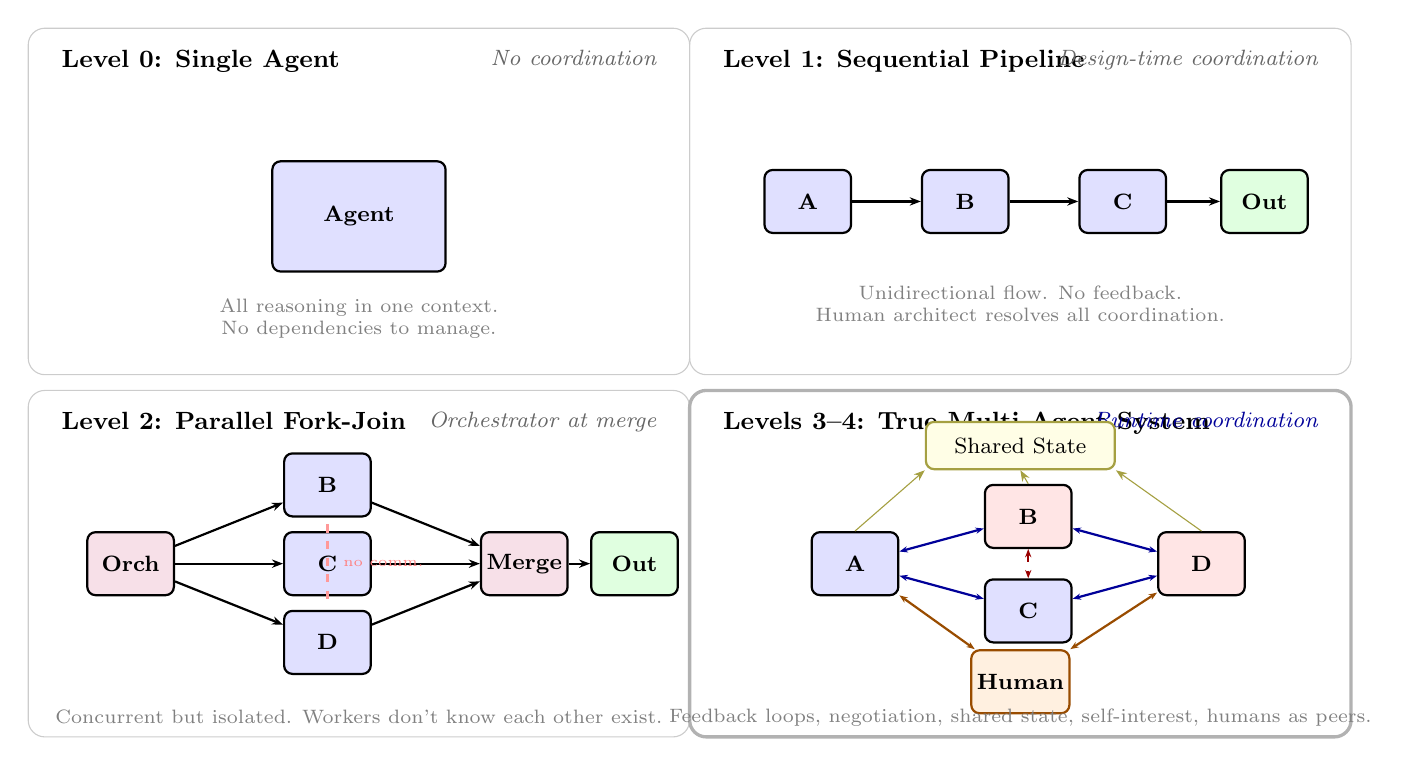
\begin{tikzpicture}[
  agent/.style={draw, thick, rounded corners=3pt, minimum width=1.1cm,
    minimum height=0.8cm, font=\footnotesize\bfseries, inner sep=2pt},
  human/.style={draw, thick, rounded corners=3pt, minimum width=1.1cm,
    minimum height=0.8cm, font=\footnotesize\bfseries, inner sep=2pt,
    fill=orange!12, draw=orange!60!black},
  shared/.style={draw, thick, rounded corners=3pt,
    minimum width=2.4cm, minimum height=0.6cm,
    font=\footnotesize, inner sep=2pt, fill=yellow!10,
    draw=yellow!60!black},
  flow/.style={-{Stealth[length=4pt, width=3pt]}, thick},
  biflow/.style={{Stealth[length=3pt]}-{Stealth[length=3pt]}, thick,
    blue!60!black},
  feedback/.style={{Stealth[length=3pt]}-{Stealth[length=3pt]}, thick,
    red!60!black, dashed},
  panellabel/.style={font=\small\bfseries, anchor=north west},
  levellabel/.style={font=\footnotesize\itshape, text=black!60},
]

% ── Panel positions ──────────────────────────────────────
\def\panelW{7.8}  % panel width
\def\panelH{3.8}  % panel height
\def\gapX{0.6}    % horizontal gap
\def\gapY{0.8}    % vertical gap

% Panel origins (bottom-left of each)
\coordinate (P0) at (0, \panelH + \gapY);
\coordinate (P1) at (\panelW + \gapX, \panelH + \gapY);
\coordinate (P2) at (0, 0);
\coordinate (P3) at (\panelW + \gapX, 0);

% ── Panel 0: Single Agent ───────────────────────────────
\begin{scope}[shift={(P0)}]
  \draw[black!20, rounded corners=6pt] (-0.3, -0.3)
    rectangle (\panelW + 0.3, \panelH + 0.3);
  \node[panellabel] at (0, \panelH + 0.15) {Level 0: Single Agent};
  \node[levellabel] at (\panelW, \panelH + 0.15) [anchor=north east]
    {No coordination};

  \node[agent, fill=blue!12, minimum width=2.2cm, minimum height=1.4cm]
    (a0) at (0.5*\panelW, 0.45*\panelH) {Agent};

  \node[font=\scriptsize, text=black!50, align=center]
    at (0.5*\panelW, 0.45*\panelH - 1.3)
    {All reasoning in one context.\\No dependencies to manage.};
\end{scope}

% ── Panel 1: Sequential Pipeline ────────────────────────
\begin{scope}[shift={(P1)}]
  \draw[black!20, rounded corners=6pt] (-0.3, -0.3)
    rectangle (\panelW + 0.3, \panelH + 0.3);
  \node[panellabel] at (0, \panelH + 0.15) {Level 1: Sequential Pipeline};
  \node[levellabel] at (\panelW, \panelH + 0.15) [anchor=north east]
    {Design-time coordination};

  \node[agent, fill=blue!12] (a1) at (1.2, 0.5*\panelH) {A};
  \node[agent, fill=blue!12] (b1) at (3.2, 0.5*\panelH) {B};
  \node[agent, fill=blue!12] (c1) at (5.2, 0.5*\panelH) {C};
  \node[agent, fill=green!12] (d1) at (7.0, 0.5*\panelH) {Out};

  \draw[flow] (a1) -- (b1);
  \draw[flow] (b1) -- (c1);
  \draw[flow] (c1) -- (d1);

  \node[font=\scriptsize, text=black!50, align=center]
    at (0.5*\panelW, 0.5*\panelH - 1.3)
    {Unidirectional flow. No feedback.\\Human architect resolves all coordination.};
\end{scope}

% ── Panel 2: Parallel Fork-Join ─────────────────────────
\begin{scope}[shift={(P2)}]
  \draw[black!20, rounded corners=6pt] (-0.3, -0.3)
    rectangle (\panelW + 0.3, \panelH + 0.3);
  \node[panellabel] at (0, \panelH + 0.15) {Level 2: Parallel Fork-Join};
  \node[levellabel] at (\panelW, \panelH + 0.15) [anchor=north east]
    {Orchestrator at merge};

  \node[agent, fill=purple!12] (orch2) at (1.0, 0.5*\panelH) {Orch};
  \node[agent, fill=blue!12] (w2a) at (3.5, 0.5*\panelH + 1.0) {B};
  \node[agent, fill=blue!12] (w2b) at (3.5, 0.5*\panelH) {C};
  \node[agent, fill=blue!12] (w2c) at (3.5, 0.5*\panelH - 1.0) {D};
  \node[agent, fill=purple!12] (merge2) at (6.0, 0.5*\panelH) {Merge};
  \node[agent, fill=green!12] (out2) at (7.4, 0.5*\panelH) {Out};

  \draw[flow] (orch2) -- (w2a);
  \draw[flow] (orch2) -- (w2b);
  \draw[flow] (orch2) -- (w2c);
  \draw[flow] (w2a) -- (merge2);
  \draw[flow] (w2b) -- (merge2);
  \draw[flow] (w2c) -- (merge2);
  \draw[flow] (merge2) -- (out2);

  % No inter-worker communication
  \draw[thick, red!40, dashed] (3.5, 0.5*\panelH + 0.5)
    -- node[font=\tiny, text=red!50, right, xshift=2pt] {no comm.}
    (3.5, 0.5*\panelH - 0.5);

  \node[font=\scriptsize, text=black!50, align=center]
    at (0.5*\panelW, -0.05)
    {Concurrent but isolated. Workers don't know each other exist.};
\end{scope}

% ── Panel 3: True MAS (Levels 3-4) ─────────────────────
\begin{scope}[shift={(P3)}]
  \draw[black!30, rounded corners=6pt, line width=1.2pt] (-0.3, -0.3)
    rectangle (\panelW + 0.3, \panelH + 0.3);
  \node[panellabel] at (0, \panelH + 0.15)
    {Levels 3--4: True Multi-Agent System};
  \node[levellabel, text=blue!60!black] at (\panelW, \panelH + 0.15)
    [anchor=north east] {Runtime coordination};

  % Shared state
  \node[shared] (ss) at (0.5*\panelW, 0.5*\panelH + 1.5)
    {Shared State};

  % Agents
  \node[agent, fill=blue!12] (ma) at (1.8, 0.5*\panelH) {A};
  \node[agent, fill=red!10] (mb) at (4.0, 0.5*\panelH + 0.6) {B};
  \node[agent, fill=blue!12] (mc) at (4.0, 0.5*\panelH - 0.6) {C};
  \node[agent, fill=red!10] (md) at (6.2, 0.5*\panelH) {D};

  % Human
  \node[human] (mh) at (0.5*\panelW, 0.5*\panelH - 1.5) {Human};

  % Bidirectional agent communication
  \draw[biflow] (ma) -- (mb);
  \draw[biflow] (ma) -- (mc);
  \draw[biflow] (mb) -- (md);
  \draw[biflow] (mc) -- (md);
  \draw[feedback] (mb) -- (mc);

  % Shared state connections
  \draw[flow, yellow!60!black, thin] (ma.north) -- (ss.south west);
  \draw[flow, yellow!60!black, thin] (mb.north) -- (ss.south);
  \draw[flow, yellow!60!black, thin] (md.north) -- (ss.south east);

  % Human connections
  \draw[biflow, orange!60!black] (mh) -- (ma);
  \draw[biflow, orange!60!black] (mh) -- (md);

  \node[font=\scriptsize, text=black!50, align=center]
    at (0.5*\panelW, -0.05)
    {Feedback loops, negotiation, shared state, self-interest, humans as peers.};
\end{scope}

\end{tikzpicture}
\caption{\textbf{The coordination complexity spectrum.}
  \emph{Level~0}: a single agent handles all reasoning in one context.
  \emph{Level~1}: agents execute sequentially with unidirectional flow; all
  coordination is resolved by the human architect at design time (adapted
  from~\citealt{cognition2025dontbuild}).
  \emph{Level~2}: subagents execute concurrently but cannot communicate with
  each other; the orchestrator handles coordination at merge (adapted
  from~\citealt{cognition2025dontbuild}).
  \emph{Levels~3--4}: true multi-agent systems with runtime dependencies,
  bidirectional communication (blue), feedback loops (red dashed), shared state
  (yellow), self-interested agents (red-tinted), and humans participating as
  peers (orange).  Classical MAS research studied Levels~3--4.  Most current
  LLM agent frameworks operate at Levels~1--2.}
\label{fig:coord-levels}
\end{figure*}


\begin{figure*}[t]
\centering
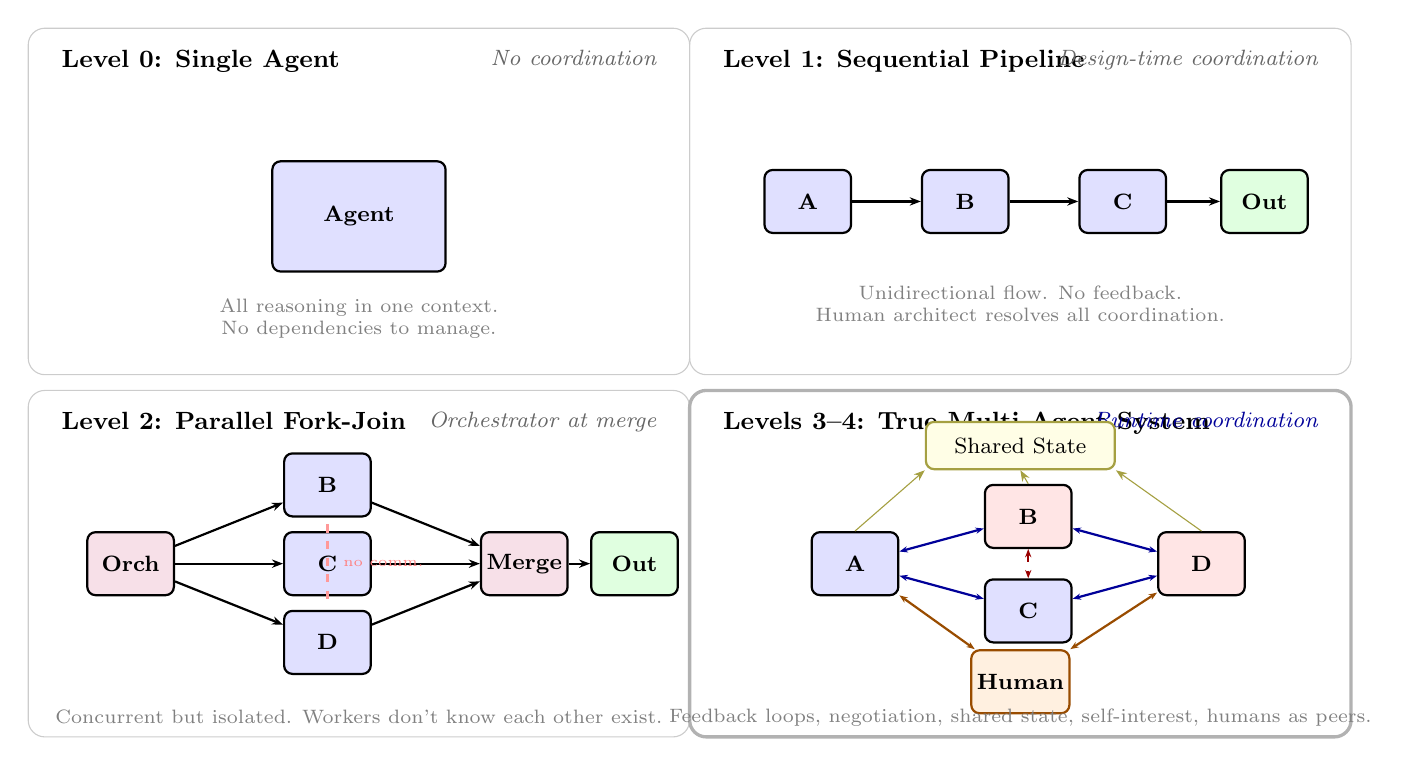
\begin{tikzpicture}[
  agent/.style={draw, thick, rounded corners=3pt, minimum width=1.1cm,
    minimum height=0.8cm, font=\footnotesize\bfseries, inner sep=2pt},
  human/.style={draw, thick, rounded corners=3pt, minimum width=1.1cm,
    minimum height=0.8cm, font=\footnotesize\bfseries, inner sep=2pt,
    fill=orange!12, draw=orange!60!black},
  shared/.style={draw, thick, rounded corners=3pt,
    minimum width=2.4cm, minimum height=0.6cm,
    font=\footnotesize, inner sep=2pt, fill=yellow!10,
    draw=yellow!60!black},
  flow/.style={-{Stealth[length=4pt, width=3pt]}, thick},
  biflow/.style={{Stealth[length=3pt]}-{Stealth[length=3pt]}, thick,
    blue!60!black},
  feedback/.style={{Stealth[length=3pt]}-{Stealth[length=3pt]}, thick,
    red!60!black, dashed},
  panellabel/.style={font=\small\bfseries, anchor=north west},
  levellabel/.style={font=\footnotesize\itshape, text=black!60},
]

% ── Panel positions ──────────────────────────────────────
\def\panelW{7.8}  % panel width
\def\panelH{3.8}  % panel height
\def\gapX{0.6}    % horizontal gap
\def\gapY{0.8}    % vertical gap

% Panel origins (bottom-left of each)
\coordinate (P0) at (0, \panelH + \gapY);
\coordinate (P1) at (\panelW + \gapX, \panelH + \gapY);
\coordinate (P2) at (0, 0);
\coordinate (P3) at (\panelW + \gapX, 0);

% ── Panel 0: Single Agent ───────────────────────────────
\begin{scope}[shift={(P0)}]
  \draw[black!20, rounded corners=6pt] (-0.3, -0.3)
    rectangle (\panelW + 0.3, \panelH + 0.3);
  \node[panellabel] at (0, \panelH + 0.15) {Level 0: Single Agent};
  \node[levellabel] at (\panelW, \panelH + 0.15) [anchor=north east]
    {No coordination};

  \node[agent, fill=blue!12, minimum width=2.2cm, minimum height=1.4cm]
    (a0) at (0.5*\panelW, 0.45*\panelH) {Agent};

  \node[font=\scriptsize, text=black!50, align=center]
    at (0.5*\panelW, 0.45*\panelH - 1.3)
    {All reasoning in one context.\\No dependencies to manage.};
\end{scope}

% ── Panel 1: Sequential Pipeline ────────────────────────
\begin{scope}[shift={(P1)}]
  \draw[black!20, rounded corners=6pt] (-0.3, -0.3)
    rectangle (\panelW + 0.3, \panelH + 0.3);
  \node[panellabel] at (0, \panelH + 0.15) {Level 1: Sequential Pipeline};
  \node[levellabel] at (\panelW, \panelH + 0.15) [anchor=north east]
    {Design-time coordination};

  \node[agent, fill=blue!12] (a1) at (1.2, 0.5*\panelH) {A};
  \node[agent, fill=blue!12] (b1) at (3.2, 0.5*\panelH) {B};
  \node[agent, fill=blue!12] (c1) at (5.2, 0.5*\panelH) {C};
  \node[agent, fill=green!12] (d1) at (7.0, 0.5*\panelH) {Out};

  \draw[flow] (a1) -- (b1);
  \draw[flow] (b1) -- (c1);
  \draw[flow] (c1) -- (d1);

  \node[font=\scriptsize, text=black!50, align=center]
    at (0.5*\panelW, 0.5*\panelH - 1.3)
    {Unidirectional flow. No feedback.\\Human architect resolves all coordination.};
\end{scope}

% ── Panel 2: Parallel Fork-Join ─────────────────────────
\begin{scope}[shift={(P2)}]
  \draw[black!20, rounded corners=6pt] (-0.3, -0.3)
    rectangle (\panelW + 0.3, \panelH + 0.3);
  \node[panellabel] at (0, \panelH + 0.15) {Level 2: Parallel Fork-Join};
  \node[levellabel] at (\panelW, \panelH + 0.15) [anchor=north east]
    {Orchestrator at merge};

  \node[agent, fill=purple!12] (orch2) at (1.0, 0.5*\panelH) {Orch};
  \node[agent, fill=blue!12] (w2a) at (3.5, 0.5*\panelH + 1.0) {B};
  \node[agent, fill=blue!12] (w2b) at (3.5, 0.5*\panelH) {C};
  \node[agent, fill=blue!12] (w2c) at (3.5, 0.5*\panelH - 1.0) {D};
  \node[agent, fill=purple!12] (merge2) at (6.0, 0.5*\panelH) {Merge};
  \node[agent, fill=green!12] (out2) at (7.4, 0.5*\panelH) {Out};

  \draw[flow] (orch2) -- (w2a);
  \draw[flow] (orch2) -- (w2b);
  \draw[flow] (orch2) -- (w2c);
  \draw[flow] (w2a) -- (merge2);
  \draw[flow] (w2b) -- (merge2);
  \draw[flow] (w2c) -- (merge2);
  \draw[flow] (merge2) -- (out2);

  % No inter-worker communication
  \draw[thick, red!40, dashed] (3.5, 0.5*\panelH + 0.5)
    -- node[font=\tiny, text=red!50, right, xshift=2pt] {no comm.}
    (3.5, 0.5*\panelH - 0.5);

  \node[font=\scriptsize, text=black!50, align=center]
    at (0.5*\panelW, -0.05)
    {Concurrent but isolated. Workers don't know each other exist.};
\end{scope}

% ── Panel 3: True MAS (Levels 3-4) ─────────────────────
\begin{scope}[shift={(P3)}]
  \draw[black!30, rounded corners=6pt, line width=1.2pt] (-0.3, -0.3)
    rectangle (\panelW + 0.3, \panelH + 0.3);
  \node[panellabel] at (0, \panelH + 0.15)
    {Levels 3--4: True Multi-Agent System};
  \node[levellabel, text=blue!60!black] at (\panelW, \panelH + 0.15)
    [anchor=north east] {Runtime coordination};

  % Shared state
  \node[shared] (ss) at (0.5*\panelW, 0.5*\panelH + 1.5)
    {Shared State};

  % Agents
  \node[agent, fill=blue!12] (ma) at (1.8, 0.5*\panelH) {A};
  \node[agent, fill=red!10] (mb) at (4.0, 0.5*\panelH + 0.6) {B};
  \node[agent, fill=blue!12] (mc) at (4.0, 0.5*\panelH - 0.6) {C};
  \node[agent, fill=red!10] (md) at (6.2, 0.5*\panelH) {D};

  % Human
  \node[human] (mh) at (0.5*\panelW, 0.5*\panelH - 1.5) {Human};

  % Bidirectional agent communication
  \draw[biflow] (ma) -- (mb);
  \draw[biflow] (ma) -- (mc);
  \draw[biflow] (mb) -- (md);
  \draw[biflow] (mc) -- (md);
  \draw[feedback] (mb) -- (mc);

  % Shared state connections
  \draw[flow, yellow!60!black, thin] (ma.north) -- (ss.south west);
  \draw[flow, yellow!60!black, thin] (mb.north) -- (ss.south);
  \draw[flow, yellow!60!black, thin] (md.north) -- (ss.south east);

  % Human connections
  \draw[biflow, orange!60!black] (mh) -- (ma);
  \draw[biflow, orange!60!black] (mh) -- (md);

  \node[font=\scriptsize, text=black!50, align=center]
    at (0.5*\panelW, -0.05)
    {Feedback loops, negotiation, shared state, self-interest, humans as peers.};
\end{scope}

\end{tikzpicture}
\caption{\textbf{The coordination complexity spectrum.}
  \emph{Level~0}: a single agent handles all reasoning in one context.
  \emph{Level~1}: agents execute sequentially with unidirectional flow; all
  coordination is resolved by the human architect at design time (adapted
  from~\citealt{cognition2025dontbuild}).
  \emph{Level~2}: subagents execute concurrently but cannot communicate with
  each other; the orchestrator handles coordination at merge (adapted
  from~\citealt{cognition2025dontbuild}).
  \emph{Levels~3--4}: true multi-agent systems with runtime dependencies,
  bidirectional communication (blue), feedback loops (red dashed), shared state
  (yellow), self-interested agents (red-tinted), and humans participating as
  peers (orange).  Classical MAS research studied Levels~3--4.  Most current
  LLM agent frameworks operate at Levels~1--2.}
\label{fig:coord-levels}
\end{figure*}


\begin{figure*}[t]
\centering
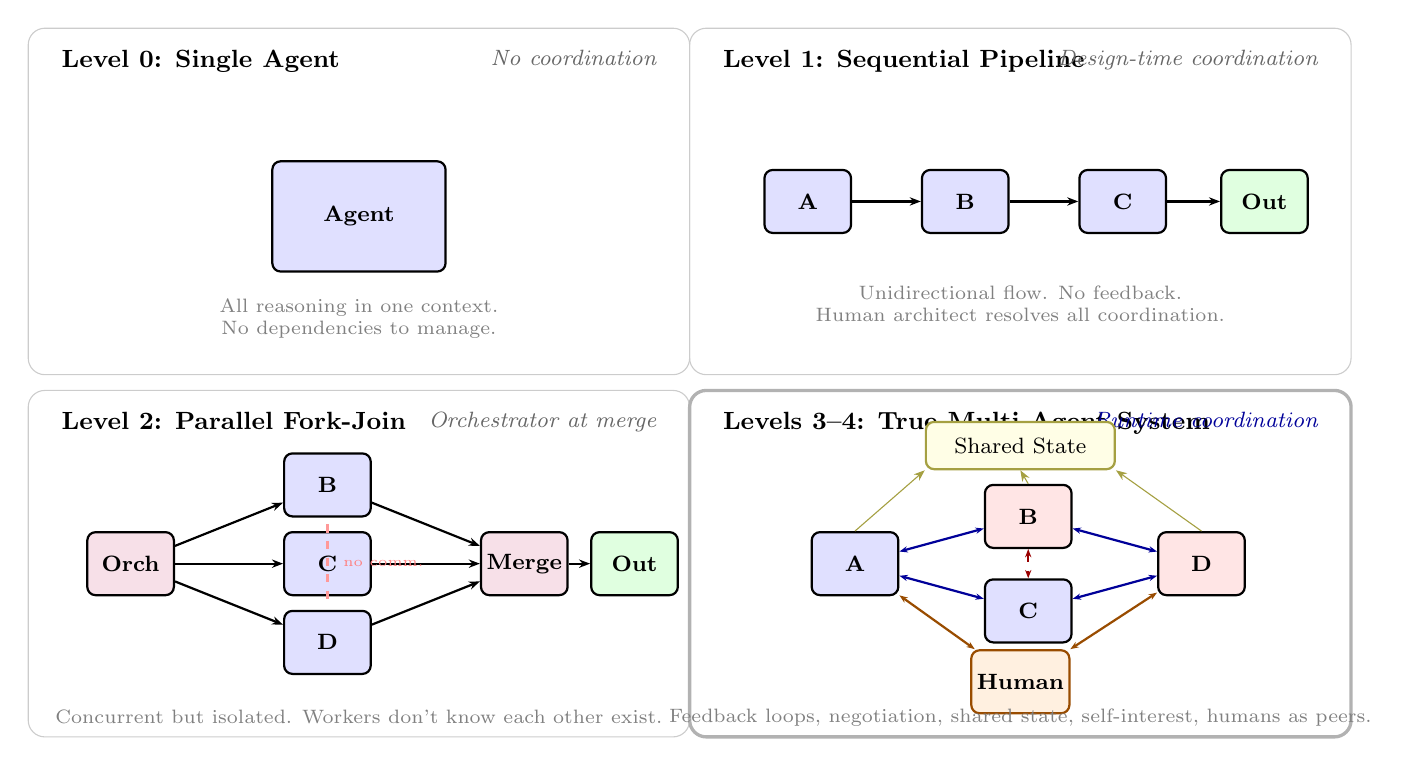
\begin{tikzpicture}[
  agent/.style={draw, thick, rounded corners=3pt, minimum width=1.1cm,
    minimum height=0.8cm, font=\footnotesize\bfseries, inner sep=2pt},
  human/.style={draw, thick, rounded corners=3pt, minimum width=1.1cm,
    minimum height=0.8cm, font=\footnotesize\bfseries, inner sep=2pt,
    fill=orange!12, draw=orange!60!black},
  shared/.style={draw, thick, rounded corners=3pt,
    minimum width=2.4cm, minimum height=0.6cm,
    font=\footnotesize, inner sep=2pt, fill=yellow!10,
    draw=yellow!60!black},
  flow/.style={-{Stealth[length=4pt, width=3pt]}, thick},
  biflow/.style={{Stealth[length=3pt]}-{Stealth[length=3pt]}, thick,
    blue!60!black},
  feedback/.style={{Stealth[length=3pt]}-{Stealth[length=3pt]}, thick,
    red!60!black, dashed},
  panellabel/.style={font=\small\bfseries, anchor=north west},
  levellabel/.style={font=\footnotesize\itshape, text=black!60},
]

% ── Panel positions ──────────────────────────────────────
\def\panelW{7.8}  % panel width
\def\panelH{3.8}  % panel height
\def\gapX{0.6}    % horizontal gap
\def\gapY{0.8}    % vertical gap

% Panel origins (bottom-left of each)
\coordinate (P0) at (0, \panelH + \gapY);
\coordinate (P1) at (\panelW + \gapX, \panelH + \gapY);
\coordinate (P2) at (0, 0);
\coordinate (P3) at (\panelW + \gapX, 0);

% ── Panel 0: Single Agent ───────────────────────────────
\begin{scope}[shift={(P0)}]
  \draw[black!20, rounded corners=6pt] (-0.3, -0.3)
    rectangle (\panelW + 0.3, \panelH + 0.3);
  \node[panellabel] at (0, \panelH + 0.15) {Level 0: Single Agent};
  \node[levellabel] at (\panelW, \panelH + 0.15) [anchor=north east]
    {No coordination};

  \node[agent, fill=blue!12, minimum width=2.2cm, minimum height=1.4cm]
    (a0) at (0.5*\panelW, 0.45*\panelH) {Agent};

  \node[font=\scriptsize, text=black!50, align=center]
    at (0.5*\panelW, 0.45*\panelH - 1.3)
    {All reasoning in one context.\\No dependencies to manage.};
\end{scope}

% ── Panel 1: Sequential Pipeline ────────────────────────
\begin{scope}[shift={(P1)}]
  \draw[black!20, rounded corners=6pt] (-0.3, -0.3)
    rectangle (\panelW + 0.3, \panelH + 0.3);
  \node[panellabel] at (0, \panelH + 0.15) {Level 1: Sequential Pipeline};
  \node[levellabel] at (\panelW, \panelH + 0.15) [anchor=north east]
    {Design-time coordination};

  \node[agent, fill=blue!12] (a1) at (1.2, 0.5*\panelH) {A};
  \node[agent, fill=blue!12] (b1) at (3.2, 0.5*\panelH) {B};
  \node[agent, fill=blue!12] (c1) at (5.2, 0.5*\panelH) {C};
  \node[agent, fill=green!12] (d1) at (7.0, 0.5*\panelH) {Out};

  \draw[flow] (a1) -- (b1);
  \draw[flow] (b1) -- (c1);
  \draw[flow] (c1) -- (d1);

  \node[font=\scriptsize, text=black!50, align=center]
    at (0.5*\panelW, 0.5*\panelH - 1.3)
    {Unidirectional flow. No feedback.\\Human architect resolves all coordination.};
\end{scope}

% ── Panel 2: Parallel Fork-Join ─────────────────────────
\begin{scope}[shift={(P2)}]
  \draw[black!20, rounded corners=6pt] (-0.3, -0.3)
    rectangle (\panelW + 0.3, \panelH + 0.3);
  \node[panellabel] at (0, \panelH + 0.15) {Level 2: Parallel Fork-Join};
  \node[levellabel] at (\panelW, \panelH + 0.15) [anchor=north east]
    {Orchestrator at merge};

  \node[agent, fill=purple!12] (orch2) at (1.0, 0.5*\panelH) {Orch};
  \node[agent, fill=blue!12] (w2a) at (3.5, 0.5*\panelH + 1.0) {B};
  \node[agent, fill=blue!12] (w2b) at (3.5, 0.5*\panelH) {C};
  \node[agent, fill=blue!12] (w2c) at (3.5, 0.5*\panelH - 1.0) {D};
  \node[agent, fill=purple!12] (merge2) at (6.0, 0.5*\panelH) {Merge};
  \node[agent, fill=green!12] (out2) at (7.4, 0.5*\panelH) {Out};

  \draw[flow] (orch2) -- (w2a);
  \draw[flow] (orch2) -- (w2b);
  \draw[flow] (orch2) -- (w2c);
  \draw[flow] (w2a) -- (merge2);
  \draw[flow] (w2b) -- (merge2);
  \draw[flow] (w2c) -- (merge2);
  \draw[flow] (merge2) -- (out2);

  % No inter-worker communication
  \draw[thick, red!40, dashed] (3.5, 0.5*\panelH + 0.5)
    -- node[font=\tiny, text=red!50, right, xshift=2pt] {no comm.}
    (3.5, 0.5*\panelH - 0.5);

  \node[font=\scriptsize, text=black!50, align=center]
    at (0.5*\panelW, -0.05)
    {Concurrent but isolated. Workers don't know each other exist.};
\end{scope}

% ── Panel 3: True MAS (Levels 3-4) ─────────────────────
\begin{scope}[shift={(P3)}]
  \draw[black!30, rounded corners=6pt, line width=1.2pt] (-0.3, -0.3)
    rectangle (\panelW + 0.3, \panelH + 0.3);
  \node[panellabel] at (0, \panelH + 0.15)
    {Levels 3--4: True Multi-Agent System};
  \node[levellabel, text=blue!60!black] at (\panelW, \panelH + 0.15)
    [anchor=north east] {Runtime coordination};

  % Shared state
  \node[shared] (ss) at (0.5*\panelW, 0.5*\panelH + 1.5)
    {Shared State};

  % Agents
  \node[agent, fill=blue!12] (ma) at (1.8, 0.5*\panelH) {A};
  \node[agent, fill=red!10] (mb) at (4.0, 0.5*\panelH + 0.6) {B};
  \node[agent, fill=blue!12] (mc) at (4.0, 0.5*\panelH - 0.6) {C};
  \node[agent, fill=red!10] (md) at (6.2, 0.5*\panelH) {D};

  % Human
  \node[human] (mh) at (0.5*\panelW, 0.5*\panelH - 1.5) {Human};

  % Bidirectional agent communication
  \draw[biflow] (ma) -- (mb);
  \draw[biflow] (ma) -- (mc);
  \draw[biflow] (mb) -- (md);
  \draw[biflow] (mc) -- (md);
  \draw[feedback] (mb) -- (mc);

  % Shared state connections
  \draw[flow, yellow!60!black, thin] (ma.north) -- (ss.south west);
  \draw[flow, yellow!60!black, thin] (mb.north) -- (ss.south);
  \draw[flow, yellow!60!black, thin] (md.north) -- (ss.south east);

  % Human connections
  \draw[biflow, orange!60!black] (mh) -- (ma);
  \draw[biflow, orange!60!black] (mh) -- (md);

  \node[font=\scriptsize, text=black!50, align=center]
    at (0.5*\panelW, -0.05)
    {Feedback loops, negotiation, shared state, self-interest, humans as peers.};
\end{scope}

\end{tikzpicture}
\caption{\textbf{The coordination complexity spectrum.}
  \emph{Level~0}: a single agent handles all reasoning in one context.
  \emph{Level~1}: agents execute sequentially with unidirectional flow; all
  coordination is resolved by the human architect at design time (adapted
  from~\citealt{cognition2025dontbuild}).
  \emph{Level~2}: subagents execute concurrently but cannot communicate with
  each other; the orchestrator handles coordination at merge (adapted
  from~\citealt{cognition2025dontbuild}).
  \emph{Levels~3--4}: true multi-agent systems with runtime dependencies,
  bidirectional communication (blue), feedback loops (red dashed), shared state
  (yellow), self-interested agents (red-tinted), and humans participating as
  peers (orange).  Classical MAS research studied Levels~3--4.  Most current
  LLM agent frameworks operate at Levels~1--2.}
\label{fig:coord-levels}
\end{figure*}


\noindent
At Level~1, Cognition's recommended architecture~\citep{cognition2025dontbuild}, an
agent's output feeds the next agent through a predetermined, unidirectional flow.
All coordination is resolved at design time by the human architect.  There is no
feedback, no negotiation, no adaptation.  At Level~2, subagents execute concurrently
but do not communicate with each other during execution; the orchestrator handles
everything at merge.  Both are legitimate engineering patterns---and both are more
reliable than naive alternatives, as Cognition correctly argues.  But neither requires
coordination theory, because neither has runtime dependencies to manage.

The problems the field reports---17.2$\times$ error amplification, 40--80\% failure
rates, 36.9\% inter-agent misalignment---emerge at Levels~3 and~4, where agents share
state, allocate tasks dynamically, and interact through feedback loops whose topology
can change during execution.  Classical MAS research spent thirty years studying
Levels~3--4.  The field is stuck at Level~2 because it does not know Level~4 exists.

\paragraph{Beyond cooperation: self-interest and tension.}
Multi-agent systems need not be cooperative, and often should not be.  In a coding
environment, development agents and testing agents should have an inherent tension---each
with a self-interest that produces higher-quality output than naive agreement.  A
cooperating agent that never pushes back is an agent that lets errors through.
RLHF-induced agreeableness, which Pappu et al.~\citep{pappu2026multiagent} identify as
the cause of 0\% strong synergy, is precisely the absence of productive tension.

Multi-agent systems need not even operate within a single organization's boundary.  An
agent negotiating a refund on behalf of a customer must interact with a retailer's agent
that has its own mandate to minimize losses.  Each has private interests it cannot
disclose and shared interests it must negotiate.  We are already seeing this evolution
in our email inboxes, where both sending and reading are increasingly performed by
agents---creating agent-to-agent interactions that were never explicitly designed.

\paragraph{State boundaries and governance.}
These dynamics demand clear boundaries on what enters shared state and what remains in an
agent's private interest---a distinction the classical MAS literature formalized through
the private beliefs of BDI agents, the partitioned knowledge sources of blackboard
systems, and the sealed bids of Contract Net auctions.  Modern frameworks, which pass
entire conversation histories between agents, make no such distinction.

Cross-boundary interaction also requires governance: shared protocols and interaction
patterns that enable productive exchange without mandating cooperation at every level.
Game theory provides the analytical framework---agents as rational actors with utility
functions, Nash equilibria as stable interaction outcomes.  Contract mechanisms provide
the operational infrastructure---binding commitments, violation detection, dispute
resolution.  And humans must remain in the loop for decisions that agents cannot
legitimately make autonomously: negotiating meeting times, setting deadlines, approving
expenditures.

\paragraph{The focus of this paper.}
This coordination---runtime dependencies, self-interested interaction, state boundaries,
governance protocols, and the feedback loops from which system intelligence
emerges---is where classical MAS research made its deepest contributions, and where
modern LLM agent systems have the largest gaps.  It is the focus of this paper.

\subsection{The Gap}
\label{sec:intro-gap}
The existing literature offers two buckets and nothing in between. On one side: tool
lists (``pip install crewai'')---curated repositories of frameworks and agents with no
theory and no ``why.'' On the other: academic benchmarks (``85\% on
HumanEval'')---leaderboards and evaluations with no architecture and no ``how.'' The
missing link is why agents fail, what classical MAS research already solved, and how to
build systems that actually work. Five recent works approach this gap; none fills it:

\begin{table}[h]
\centering
\caption{Positioning against closest existing work.}
\label{tab:positioning}
\begin{tabular}{@{} p{2.2cm} p{2.2cm} p{2.8cm} @{}}
\toprule
\textbf{Existing Work} & \textbf{What It Covers} & \textbf{Gap We Fill} \\
\midrule
Cemri et al., ICLR 2025 & 14 failure modes taxonomized & Map every failure mode to a classical MAS solution \\
Kim et al., DeepMind 2025 & Centralized $>$ decentralized (data) & Explain \emph{why} using coordination theory; prescribe the Control Shell \\
``Contemporary Agent Technology'' (Sep 2025) & Diagnoses the BDI/FIPA vs.\ ReAct/CoT disconnect & Focus on organizational design and coordination failure \\
``Reliable Agent Engineering'' (Dec 2025) & Argues for organization over model size & Provide the manual---patterns, schemas, benchmarks \\
``Agent Interop Protocols'' (May 2025) & Technical protocol breakdown & Connect specs to interaction patterns (e.g., Contract Net over A2A) \\
\bottomrule
\end{tabular}
\end{table}

\subsection{Contributions}
\label{sec:intro-contributions}

This paper makes eight contributions:
\begin{enumerate}[nosep, label=\textbf{C\arabic*}:]
  \item \textbf{The Sutra Corpus}---36,013 papers (17,971 deeply annotated) processed by
    a 7-agent blackboard pipeline with structured coordination-pattern annotations
    spanning 1975--2026.
  \item \textbf{A 16-segment MAS taxonomy}---semi-supervised clustering bridging 50 years
    of research into a navigable map with reading triples (landmark, central, survey)
    per segment.
  \item \textbf{The Lost Canary Algorithm}---a citation-graph methodology for detecting
    genuinely forgotten concepts: 4 lost, 1 known-but-ignored, 8 renamed without
    citation.
  \item \textbf{The Rosetta Stone}---a classical-to-modern mapping with fidelity ratings,
    gap analysis, and protocol-level translation (FIPA ACL $\to$ A2A/MCP).
  \item \textbf{Eight Design Principles}---synthesized from organizational science,
    classical MAS theory, and production system evidence, each with falsifiable
    predictions.
  \item \textbf{Empirical validation}---9 classical patterns + 2 baselines tested across
    5 benchmarks (55+ experiments); star result: Blackboard V2 = 95/100.
  \item \textbf{Open research infrastructure}---the Sutra Portal (interactive dashboard),
    GitHub repository (structured corpus + experiment harness), and pipeline code.
  \item \textbf{Replication infrastructure}---Agent 5/6 scouting with reproduction targets
    for 6 key papers, bridging to a dedicated replication study.
\end{enumerate}

\paragraph{Computational scale.}
These contributions rest on an investment of computational analysis unprecedented for a
survey paper. The 7-agent pipeline consumed approximately \textbf{250 million tokens}
of frontier models---GPT-5.1 for deep structured extraction (Agent~3b) and Claude
Opus~4.6 for analytical assessment and cluster labeling---to analyze and annotate
${\sim}17{,}000$ papers with structured coordination-pattern metadata. A further
${\sim}100$ million tokens of GPT-5-mini were consumed to relevance-filter the full
${\sim}36{,}000$-paper candidate set. All papers were embedded using
\texttt{text-embedding-3-small} (1536 dimensions) and indexed in Azure AI Search with
hybrid keyword-vector retrieval and semantic ranking; multiple rounds of embedding,
clustering, re-clustering, and anchor refinement were required to produce the stable
16-segment taxonomy (Section~\ref{sec:meth-taxonomy}). This scale of AI-powered
literature analysis---${\sim}350$ million tokens of structured processing---transforms
the traditional survey methodology from ``expert reads papers and reports impressions''
into a computationally grounded, reproducible process where every claim traces to
structured extraction across the full corpus.

\subsection{Paper Organization}
\label{sec:intro-organization}

The remainder of this paper is organized as follows.
Section~\ref{sec:background} traces the arc of multi-agent systems from the classical era
through the lost decade to the current renaissance, quantifying the failure landscape.
Section~\ref{sec:methodology} describes the Lost Canary methodology, the 7-agent
pipeline, the experiment harness, and the reference selection algorithm.
Section~\ref{sec:taxonomy} presents the design of the 16-segment taxonomy---the
semi-supervised method and the three-generation anchor evolution that produced it.
Section~\ref{sec:pillars} surveys the 16 pillars of MAS research---the
survey-within-the-survey.
Section~\ref{sec:results} presents the Lost Canary findings, Rosetta Stone, and corpus
statistics.
Section~\ref{sec:principles} synthesizes eight design principles from organizational
science and classical MAS.
Section~\ref{sec:experiments} reports experiment results, including two star findings.
Section~\ref{sec:related} positions this work against existing surveys.
Section~\ref{sec:discussion} discusses when MAS excels, when it does not, limitations,
and open problems.
Section~\ref{sec:conclusion} concludes.


% ══════════════════════════════════════════════════════════════
% SECTION 2: BACKGROUND (~4 pages)
% Source: theoretical-foundations.md, classical-mas-llm-bridge.md,
%         evolution-from-classics-to-mcp.md, why-mas-works.md
% ══════════════════════════════════════════════════════════════
\section{Background: The Arc of Multi-Agent Systems}
\label{sec:background}

\subsection{The Classical Era (1980--2005)}
\label{sec:bg-classical}

% --- PLAN ---
% The founding problem: distributed problem solving
%   (Durfee, Lesser, Corkill)
%
% Three intellectual traditions:
%   1. The Joint Intentions School (Cohen, Levesque, Grosz, Sidner,
%      Kraus) -- formal logic of teamwork
%   2. The DAI/Cooperation Frameworks (Durfee, Lesser, Corkill, Bond,
%      Gasser) -- pragmatic distributed problem-solving
%   3. The Social/Organizational School (Singh, Fox, Jennings) -- roles,
%      commitments, conventions
%
% Key protocols:
%   - Contract Net (Smith 1980) -- announce/bid/award
%   - KQML (1993) -- first agent communication language
%   - FIPA ACL (1997-2003) -- 22 typed performatives with formal
%     semantics
%
% Key architectures:
%   - Blackboard (Nii 1986) -- shared state + knowledge sources +
%     control shell
%   - BDI (Rao & Georgeff 1995) -- beliefs/desires/intentions cycle
%
% Key theory:
%   - Coordination Theory (Malone & Crowston 1994) -- dependencies
%     determine coordination mechanisms
%   - SharedPlans (Grosz & Kraus 1996) -- mutual belief as prerequisite
%     for joint action
%   - Argumentation (Dung 1995) -- formal attack/support frameworks
%
% The peak: AAMAS founded 2002, FIPA standards ratified, JADE mature
%
% Source: theoretical-foundations.md, classical-mas-llm-bridge.md

The classical era of multi-agent systems produced three intellectual traditions that
remain relevant---and largely unread---in the LLM agent community.

\paragraph{The Joint Intentions School.}
Cohen and Levesque~\citep{cohen1990intention} formalized joint action in modal logic:
a team jointly intends an action only when each member individually intends it, each
believes the others intend it, and each is committed to informing the group if the goal
becomes unachievable. Grosz and Kraus~\citep{grosz1996collaborative} extended this into
\emph{SharedPlans}---the theory that coordination requires \emph{mutual belief}: knowing
the plan AND knowing that others know it. Tambe's STEAM~\citep{tambe1997steam}
operationalized these ideas in deployed systems. This tradition gave MAS its formal
foundations for teamwork, commitment, and the obligation to communicate failure.

\paragraph{The DAI/Cooperation Frameworks.}
Durfee, Lesser, and Corkill~\citep{lesser1983functionally, durfee1999distributed}
attacked the pragmatic problem: how do distributed systems solve problems that no single
node can solve alone? Their Functionally Accurate, Cooperative (FA/C) approach embraced
partial, tentative results exchanged early and refined iteratively
(Section~\ref{sec:p-dps}). The Generalized Partial Global Planning (GPGP)
framework~\citep{decker1995gpgp} provided coordination mechanisms matched to dependency
types---a precursor to Malone and Crowston's coordination theory. Bond and
Gasser~\citep{bond1988readings} established the intellectual agenda for Distributed
Artificial Intelligence as a field.

\paragraph{The Social/Organizational School.}
Singh~\citep{singh1999social}, Jennings~\citep{jennings2000agent}, and
Fox~\citep{fox1998organizational} argued that agents are not isolated reasoners but
social entities embedded in organizational structures with roles, commitments, and
conventions. Jennings' influential argument~\citep{jennings2000agent} that ``Agent is
above Object''---that agents possess intentionality, social ability, and organizational
membership that objects do not---remains the clearest articulation of why agent-oriented
design differs from ordinary software engineering.

\paragraph{Key protocols and architectures.}
These traditions produced concrete infrastructure. Smith's Contract Net
Protocol~\citep{smith1980contract} (1980) introduced decentralized task allocation via
announce/bid/award. KQML~\citep{finin1994kqml} (1993) provided the first agent
communication language with typed performatives. FIPA ACL~\citep{fipaacl2002}
(1997--2003) refined it with 22 performatives grounded in formal BDI semantics. The
blackboard architecture~\citep{nii1986blackboard} (Nii 1986, building on Erman et al.'s
Hearsay-II) provided shared-state coordination with a control shell. The BDI
architecture~\citep{rao1995bdi} (Rao \& Georgeff 1995) provided the cognitive loop for
rational agents.

\paragraph{Key theory.}
Malone and Crowston's coordination theory~\citep{malone1994interdisciplinary} (1994)
established the foundational theorem: \emph{coordination is managing dependencies between
activities}, and the dependency type determines the coordination mechanism. Dung's
abstract argumentation~\citep{dung1995acceptability} (1995) provided formal frameworks
for structured disagreement. Hoare's CSP~\citep{hoare1978communicating} (1978) and
Milner's pi-calculus~\citep{milner1992calculus} (1992) provided process algebras for
specifying and verifying concurrent agent interactions---CSP enables automated deadlock
checking, while the pi-calculus adds channel mobility for dynamic topology
reconfiguration. Hewitt's Actor Model~\citep{hewitt1973actor} (1973), operationalized
through Erlang/OTP~\citep{armstrong2003erlang}, contributed supervision trees and the
principle that error handling must be separated from error detection.

From distributed systems theory, Brewer's CAP theorem provides a fundamental framing for
multi-agent architectures: a distributed system cannot simultaneously guarantee
Consistency, Availability, and Partition Tolerance. For agents, consistency means all
agents see the same context (requiring synchronization barriers), availability means
agents respond without waiting (potentially acting on stale context), and partition
tolerance means agents handle API failures. The PACELC extension adds the
Latency-Consistency tradeoff even without partitions: centralized architectures (PC/EC)
trade latency for consistency (4.4$\times$ error amplification), while independent
architectures (PA/EL) trade consistency for speed (17.2$\times$ error). This provides
the theoretical explanation for Kim et al.'s empirical findings
(Section~\ref{sec:bg-failures}).

\paragraph{The peak.}
By the early 2000s, the field had matured. AAMAS was founded in 2002, unifying
the Agents and ICMAS communities. FIPA standards were ratified. JADE provided a
production-quality implementation. The intellectual infrastructure was in place. Then the
world stopped paying attention.

\subsection{The Lost Decade (2006--2022)}
\label{sec:bg-lost}

% --- PLAN ---
% AlexNet (2012) -> Transformers (2017) -> GPT-3 (2020):
%   attention and funding shift to scaling single models
%
% MAS research continues (AAMAS, JAAMAS) but loses mainstream
% visibility
%
% The citation cliff begins: root primitives accumulate total citations
% but modernity scores drop below 0.05
%
% JADE stops maintenance (2021). FIPA effectively dormant.
%
% Key data: era distribution from corpus shows 2010s = 12.2%
% (the trough -- visible evidence of the citation disconnect this
% paper studies)
%
% Source: modernity_scores.json, era distribution from corpus

The deep learning revolution---AlexNet (2012), Transformers~\citep{vaswani2017attention}
(2017), GPT-3~\citep{brown2020language} (2020)---redirected the attention and funding of
the AI community toward scaling single models on single tasks. Multi-agent systems
research continued at AAMAS and in JAAMAS, but it lost mainstream visibility. In our
corpus, the 2010s account for only 12.2\% of papers---the trough between the golden age
of classical MAS (2000s: 34.4\%) and the LLM agent explosion (2025+: 26.3\%). This
trough is the visible evidence of the citation disconnect this paper studies.

The infrastructure decayed alongside the attention. JADE (Java Agent Development
Framework)~\citep{bellifemine2007jade}, the gold standard for FIPA-compliant multi-agent
development throughout the 2000s, saw its original team stop maintenance in 2021. A
community fork~\citep{jadeplatform} preserves compatibility with Java~17 but adds no new
capabilities. FIPA itself became effectively dormant---its standards remain ratified but
unenforced, its working groups inactive.

The citation cliff begins in this period. Our modernity score analysis
(Section~\ref{sec:meth-canary}) shows that root primitives---foundational concepts like
the Contract Net Protocol, SharedPlans, and the BDI architecture---continue to accumulate
total citations but their modernity scores (the fraction of citations from 2023--2026)
drop below 0.05. The concepts are still referenced in surveys and textbooks, but they are
no longer \emph{used} in new system designs. They are remembered in the library but
forgotten in the laboratory.

\subsection{The LLM Agent Renaissance (2023--2026)}
\label{sec:bg-renaissance}

% --- PLAN ---
% Framework explosion:
%   - AutoGen (2023), CrewAI (2024), LangGraph (2024),
%     Google ADK (2025)
%
% The protocol stack emerges:
%   - MCP (agent-to-tool, Anthropic)
%   - A2A (agent-to-agent, Google)
%   - ANP (discovery, W3C DID)
%
% The 2025+ surge: 26.3% of our corpus is from 2025+
%
% Production deployments: Anthropic, Cognition Devin, ChatDev, MetaGPT
%
% But: building from scratch, ignoring 30 years of theory
%
% The bifurcation: classical researchers extend toward LLMs (ChatBDI,
%   NatBDI, SPADE) while framework developers build from scratch --
%   two communities, same problem, zero cross-pollination
%
% Source: evolution-from-classics-to-mcp.md, classical-mas-llm-bridge.md

The arrival of capable language models---GPT-4~\citep{openai2023gpt4} in March 2023,
Claude~3 in March 2024, and their successors---triggered a framework explosion.
AutoGen~\citep{wu2023autogen} (2023), CrewAI (2024), LangGraph~\citep{langgraph2024}
(2024), and Google's Agent Development Kit~\citep{googleadk2025} (2025) appeared in rapid
succession, each providing multi-agent coordination infrastructure for LLMs. In our
corpus, 26.3\% of papers are from 2025 or later---the LLM agent renaissance is
generating research at a rate that exceeds the entire 2010s combined.

Alongside the frameworks, a protocol stack is crystallizing:
\begin{itemize}[nosep]
  \item \textbf{MCP} (Model Context Protocol, Anthropic): agent-to-tool communication,
    standardizing how agents invoke external capabilities.
  \item \textbf{A2A} (Agent-to-Agent, Google): inter-agent communication with task
    lifecycle management, agent cards for capability advertisement.
  \item \textbf{ANP} (Agent Network Protocol): decentralized agent discovery using W3C
    Decentralized Identifiers.
\end{itemize}
Production deployments are scaling: Anthropic's multi-agent research
system~\citep{anthropic2025building}, Cognition's Devin, MetaGPT~\citep{hong2024metagpt},
and ChatDev~\citep{qian2024chatdev} demonstrate that multi-agent coordination can deliver
real-world value when the coordination infrastructure is sound.

\paragraph{The bifurcation.}
The field is characterized by a striking disconnect. On one side, classical MAS
researchers extend their frameworks toward LLMs: ChatBDI~\citep{chatbdi2025} adds
natural language to Jason/JaCaMo agents, SPADE~4.0~\citep{palanca2020spade} maintains
FIPA compliance in Python with async support, and a growing body of work maps BDI
concepts onto LLM architectures (Section~\ref{sec:p-bdi}). On the other side, LLM
framework developers build from scratch, ignoring thirty years of agent theory---two
communities working on the same problem with near-zero cross-pollination. This paper
is an attempt to thread the two traditions together.

\paragraph{A recurring pattern.}
Knowledge loss during paradigm shifts is not unique to multi-agent systems.
The Gang of Four's \emph{Design Patterns}~\citep{gamma1994design} mapped recurring
solutions from Christopher Alexander's architectural pattern
language~\citep{alexander1977pattern} to object-oriented software---a Rosetta Stone
between fields separated by decades and disciplinary boundaries.  The neural network
community experienced two ``winters'' where connectionist ideas were forgotten and
independently rediscovered: Rosenblatt's perceptron (1958) was buried by Minsky and
Papert's critique (1969), only to resurface with backpropagation in the 1980s, then
fade again before deep learning's post-2012 explosion.  In aviation, Helmreich's
cockpit resource management protocols~\citep{helmreich1999cockpit}---which reduced
accidents by over 50\%---took twenty years to transfer to surgical teams, where
Gawande~\citep{gawande2011checklist} demonstrated the same structured communication
principles could reduce fatalities by 33\%.  Sutton's ``Bitter
Lesson''~\citep{sutton2019bitter} argues that the field \emph{repeatedly} forgets that
general-purpose methods leveraging computation beat hand-engineered solutions---the
opposite direction from our argument, but the same pattern of cyclical amnesia.  In
each case, the mechanism is identical: a paradigm shift redirects attention, and
practitioners in the new paradigm build from scratch rather than inheriting from the
old.  The Lost Canary methodology (Section~\ref{sec:meth-canary}) is an attempt to
detect and quantify this phenomenon systematically.

\subsection{The Failure Landscape (Quantified)}
\label{sec:bg-failures}

% --- PLAN ---
% Cemri et al.'s 14 failure modes across 3 categories:
%   FC1: Specification & Design
%   FC2: Inter-Agent (36.9% of failures from misalignment)
%   FC3: Verification & Validation
%   Overall: 40-80% failure rate
%
% Kim et al.'s 180 configurations:
%   - 17.2x error amplification (independent agents)
%   - 4.4x error amplification (centralized)
%   - Hybrid topologies outperform both extremes
%
% The 45% capability ceiling -- single-agent accuracy above which
% adding agents starts to hurt
%
% The sequential penalty: 39-70% degradation on sequential tasks
%
% The 87% architecture prediction accuracy from task features alone --
%   key insight: topology is predictable from task structure, not
%   something you discover by trial and error
%
% Key insight: "failures require more complex solutions" -- not prompt
% fixes but organizational design
%
% Source: why-mas-works.md (The Numbers section)

\paragraph{The Cemri taxonomy.}
Cemri et al.~\citep{cemri2025fail} analyzed failures across multiple LLM agent
systems and identified 14 unique failure modes in three categories:

\begin{itemize}[nosep]
  \item \textbf{FC1: Specification \& System Design} (5 modes)---task specification
    violations, role confusion, step repetition, lost conversation history, unawareness
    of termination conditions.
  \item \textbf{FC2: Inter-Agent Misalignment} (6 modes)---conversation reset, failure
    to request clarification, task derailment, information withholding, disregarding
    other agent input, reasoning-action mismatch. This category accounts for 36.9\%
    of all failures.
  \item \textbf{FC3: Task Verification \& Termination} (3 modes)---premature
    termination, incomplete verification, incorrect verification.
\end{itemize}

\noindent
The critical finding is that ``identified failures require more complex
solutions''~\citep{cemri2025fail}: tactical prompt improvements yield only modest
gains (ChatDev improving from 25\% to 34.4\% after prompt fixes). Even topology
redesign reaches only 40.6\%. The failures stem from fundamental organizational
design flaws, not individual agent limitations.

\paragraph{The Kim scaling study.}
Kim et al.~\citep{kim2025scaling} tested 180 agent configurations across HumanEval,
MATH, and MMLU, producing the most comprehensive empirical picture of multi-agent
scaling:

\begin{table}[h]
\centering
\caption{Error amplification by architecture type \citep{kim2025scaling}.}
\label{tab:error-amp}
\small
\begin{tabular}{@{} p{2.6cm} c p{2.6cm} @{}}
\toprule
\textbf{Architecture} & \textbf{Error} & \textbf{When It Helps} \\
\midrule
Single-agent & 1$\times$ & Sequential; $<$45\% baseline \\
Independent & 17.2$\times$ & Never recommended \\
Centralized & 4.4$\times$ & Parallelizable (+80.9\%) \\
Decentralized & Moderate & Diverse perspectives \\
Hybrid & Best & Complex tasks \\
\bottomrule
\end{tabular}
\end{table}

\noindent
Three additional findings shape the design space. First, the \textbf{45\% capability
ceiling}: when single-agent accuracy exceeds 45\% on a non-decomposable task, adding
agents starts to hurt---the coordination overhead exceeds the diversity benefit. Second,
the \textbf{sequential penalty}: multi-agent systems degrade performance by 39--70\% on
sequential reasoning tasks. Third, the \textbf{87\% architecture prediction}: a model
trained on task features alone---decomposability, parallelism, sequential
depth---predicts the optimal topology with 87\% accuracy on unseen tasks. Topology is
predictable from task structure, not something to discover by trial and error.

\paragraph{The root causes.}
The 17.2$\times$ error amplification is not a law of nature. It traces to five specific
design failures, each of which maps to a classical MAS solution:
\begin{enumerate}[nosep]
  \item \textbf{No dependency analysis}---agents are assembled without mapping what
    depends on what (Section~\ref{sec:p-dps}).
  \item \textbf{Free-text communication}---inter-agent messages are unstructured natural
    language, not typed schemas (Section~\ref{sec:p-acl}).
  \item \textbf{No quality gates}---outputs flow from agent to agent without
    verification (Section~\ref{sec:p-eval}).
  \item \textbf{No error recovery}---when one agent fails, the failure cascades
    (Section~\ref{sec:p-aose}).
  \item \textbf{No bounded autonomy}---agents either have too much freedom (drift) or
    too little (bottleneck) (Section~\ref{sec:p-org}).
\end{enumerate}

\noindent
These are the same problems that plague badly organized human teams---and the same
problems that classical MAS research spent thirty years solving.


% ══════════════════════════════════════════════════════════════
% SECTION 3: METHODOLOGY (~5 pages)
% Source: contributions.md (preamble, C1, C2, C3, C6),
%         cointelligence/methodology.md (Agent 0)
% ══════════════════════════════════════════════════════════════
\section{Methodology}
\label{sec:methodology}

\subsection{The Two-Level Human-AI Research Architecture}
\label{sec:meth-levels}

% --- PLAN ---
% Level 1 -- Interactive Human-AI Research (Sprints r1-r2):
%   Author works directly with Claude Code through 6 custom research
%   commands, each a structured prompt with specific tool permissions
%   and output formats:
%     /research-plan  -- Sprint planning with explicit hypotheses
%     /literature     -- Citation graph traversal, Lost Canary detection
%     /experiment     -- GitHub discovery + Python test harness
%     /analyze        -- Archivist/Modernist/Bridge Builder assessment
%     /write          -- Paper section drafting
%     /research-review -- 7-phase quality gate
%   The human drives every decision; the AI executes citation traversal,
%   extraction, and structured analysis.
%
% Level 2 -- Autonomous Pipeline (Sprint r3+):
%   Informed by Level 1 findings, the author designed a scaled 7-agent
%   blackboard system running unattended on a VM. This level processed
%   36,013 papers into the 17,971-paper Sutra Corpus. The human
%   monitors, calibrates, and intervenes at quality gates.
%
% The transition: Level 1 findings informed Level 2 design.
%   The /literature command's compound filter became Agent 2's scoring
%   rubric. The /analyze command's prompt templates became the
%   Archivist/Modernist/Bridge Builder agents. The /research-review QA
%   gate became the author's sampling protocol.
%
% Self-referential note: the pipeline IS a blackboard architecture
%   studying blackboard architectures
%
% --- PLAN: Agent 0 — The Human as Peer Agent ---
% The human researcher is not a supervisor but a first-class team
% member (Agent 0) with dynamic roles that evolve across phases:
%
%   Phase            | Agent 0 Role    | What the Human Does That AI Cannot
%   Seed selection   | Architect       | Cross-disciplinary judgment: which 33
%                    |                 |   papers span all 6 MAS branches
%   Filtering        | Supervisor      | Rescue false negatives: Hearsay-II
%                    |                 |   scored 0, Actor model scored 3
%   Analysis         | Quality gate    | Validate extraction quality on samples,
%                    |                 |   adjust prompts
%   Feedback loop    | Safety engineer | Set generation/corpus caps, monitor
%                    |                 |   growth, disable when returns diminish
%   Scouting         | Prioritizer     | Select reproduction targets based on
%                    |                 |   thesis relevance, not citation count
%   Clustering       | Synthesizer     | Override auto-k (63->16), tune UMAP,
%                    |                 |   curate anchor descriptions
%   Writing          | Author          | Thesis, narrative arc, significance
%                    |                 |   judgment
%
% Key distinction from existing AI research systems:
%   - CrewAI assigns fixed roles. Agent 0's role is DYNAMIC.
%   - LangGraph has static graphs. The human's activation conditions
%     change per phase.
%   - AI Scientist v2 produces workshop-level papers with 42% failure.
%     The difference is not the model — it's the coordination architecture.
%
% This human-AI coordination pattern is itself an instance of the
% coordination infrastructure this paper advocates. The pipeline's
% success is evidence for the thesis. Full formalization of Agent 0
% is the subject of a companion paper (Paper 2: "Agent 0").
%
% Source: contributions.md methodology preamble,
%         cointelligence/methodology.md (Agent 0 formalization)

The Sutra research operates at two distinct levels, executed sequentially, consuming
approximately 350 million tokens of LLM inference across frontier models (GPT-5.1,
Claude Opus~4.6) and efficient models (GPT-5-mini). Each level uses different tools,
different coordination architectures, and different human roles.

\paragraph{Level 1: Interactive Human-AI Research (Sprints r1--r2).}
The author works directly with Claude Code through six custom research commands, each
a structured prompt with explicit tool permissions and output formats:

\begin{center}
\small
\begin{tabular}{@{} l l p{3.2cm} @{}}
\toprule
\textbf{Command} & \textbf{Phase} & \textbf{Purpose} \\
\midrule
\texttt{/research-plan} & Planning & Sprint planning with hypotheses \\
\texttt{/literature} & Phases 1--3 & Citation traversal, Lost Canary detection \\
\texttt{/experiment} & Validation & GitHub discovery + test harness \\
\texttt{/analyze} & Phase 5 & Archivist/Modernist/Bridge assessment \\
\texttt{/write} & Phase 7 & Section drafting with guidance \\
\texttt{/research-review} & QA & 7-phase quality gate \\
\bottomrule
\end{tabular}
\end{center}

\noindent
At this level, the human drives every decision---which concepts to investigate, which
hypotheses to test, how to interpret results. The AI executes citation traversal,
structured extraction, and analysis at a speed and breadth impossible manually.
Level~1 produced the Lost Canary algorithm, the initial seed expansion, the
backward/forward passes, and the first structured assessments.

\paragraph{Level 2: Autonomous Pipeline (Sprint r3+).}
Informed by Level~1 findings, the author designed a scaled 7-agent blackboard system
running unattended on a dedicated VM (Section~\ref{sec:meth-pipeline}). This level
processed 36,013 papers into the 17,971-paper Sutra Corpus. The human
monitors, calibrates, and intervenes at quality gates---but does not direct individual
agent actions.

The transition from Level~1 to Level~2 was deliberate: the \texttt{/literature}
command's compound filter became Agent~2's scoring rubric. The \texttt{/analyze}
command's prompt templates became the Archivist, Modernist, and Bridge Builder agents
in Phase~5. The \texttt{/research-review} QA gate became the author's sampling protocol
(Section~\ref{sec:meth-pipeline}, Step~5). Each Level~2 component has a traceable
lineage to a Level~1 prototype.

\paragraph{Agent 0: The Human as Peer Agent.}
A distinctive feature of the methodology is the human researcher's role---not an
external supervisor but a first-class team member (Agent~0) whose role evolves
dynamically across research phases:

\begin{table}[h]
\centering
\caption{Agent~0 role transitions across research phases.}
\label{tab:agent0-roles}
\small
\begin{tabular}{@{} l l p{3.5cm} @{}}
\toprule
\textbf{Phase} & \textbf{Role} & \textbf{Human Contribution} \\
\midrule
Seed selection & Architect & Cross-disciplinary judgment: 33 papers spanning 6 branches \\
Filtering & Supervisor & Rescue false negatives (Hearsay-II scored 0/10) \\
Analysis & Quality gate & Validate extraction; adjust prompts \\
Feedback loop & Safety engr. & Set caps; monitor growth; disable when returns diminish \\
Clustering & Synthesizer & Override $k{=}63$ to 16 anchors \\
Writing & Author & Thesis, narrative, significance \\
\bottomrule
\end{tabular}
\end{table}

\noindent
This dynamic role transition distinguishes the methodology from existing AI-for-research
systems. CrewAI assigns fixed roles. LangGraph has static graphs. AI Scientist~v2
produces workshop-level papers with 42\% failure~\citep{lu2024aiscientist}. The
difference is not the model---the same LLMs are available to all systems---but the
coordination architecture. The Sutra Portal's Agent~0 Console
(Section~\ref{sec:res-artifacts}) operationalizes these role transitions through 6 HCI
patterns, including cognitive forcing functions that require the researcher to commit
judgment \emph{before} seeing the AI's assessment---preventing the anchoring bias that
undermines na\"ive human-in-the-loop designs. The pipeline's success is itself evidence
for the coordination patterns this paper advocates. The full formalization of Agent~0,
including activation conditions and ablation analysis, is the subject of a companion
paper~\citep{viswanathan2026agent0}.

\subsection{The Lost Canary Algorithm}
\label{sec:meth-canary}

% --- PLAN ---
% Phase 1 -- Seed Selection:
%   22 classical + 11 modern bridge papers spanning 6 MAS branches
%   (Communication, Organization, Coordination, Architecture,
%   Negotiation, Verification)
%
% Phase 2 -- Backward Pass (Root Primitive Discovery):
%   From 22 seeds, fetch all references via OpenAlex/Semantic Scholar.
%   Score each by:
%     root_primitive_score = cite_count x branch_diversity
%     Threshold: score >= 6 (e.g., 3 citations x 2 branches)
%   Where branch_diversity = number of distinct MAS branches among
%   the seeds citing it. Ensures root primitives are foundational
%   across the field, not just dominant in one subarea.
%   Found: 18 root primitives clustered into three intellectual
%   traditions (Joint Intentions, DAI/Cooperation, Social/Org)
%
% Phase 3 -- Forward Pass (Modernity Score):
%   For each root primitive, compute citation trajectory:
%     Modernity Score = (Citations 2023-2026) / (Total Citations)
%   Threshold: Total Citations > 500 AND Modernity Score < 0.05
%     = Lost Canary Candidate
%   Result: 18 -> 6 candidates (score < 0.05), 3 active (> 0.05),
%   9 below citation threshold
%
% Phase 4 -- Concept Tracing (Anti-False-Positive):
%   Three mandatory checks before confirming any Lost Canary:
%   1. Field growth normalization: Is the low modernity score just
%      because AI grew faster than MAS?
%   2. Survey citation check: If surveys cite it but implementation
%      papers don't -> "Known but Ignored," not "Genuinely Lost"
%   3. Indirect citation check: If Survey X cites Root Primitive Y,
%      do papers citing Survey X use Y's concepts without citing Y?
%
% Phase 5 -- Multi-Perspective Assessment:
%   Archivist (classical MAS 2005 persona) / Modernist (LLM 2026
%   persona) / Bridge Builder (both literatures) + Critic (devil's
%   advocate)
%   Self-critique protocol: 4 mandatory questions per mapping:
%     1. Is the mapping genuine or superficial?
%     2. Has the problem fundamentally changed?
%     3. Counter-evidence?
%     4. Alternative explanations?
%   Each mapping receives verdict: STRONG CANARY / WEAK CANARY /
%   FALSE ALARM / GENUINELY NEW with confidence and reasoning
%
% Phase 6 -- Human Synthesis (5 irreplaceable author roles):
%   1. Narrative identification -- which Lost Canaries matter?
%   2. Thesis construction -- connecting data to argument
%   3. Significance judgment -- promoting theoretically important
%      findings over merely popular ones
%   4. Cross-contribution integration -- seeing the whole
%   5. Writing -- intro, thesis, implications, conclusion
%
% Source: contributions.md C1 and C3

The Lost Canary Algorithm is a systematic citation-graph methodology for detecting
foundational concepts that an entire research community has forgotten or is unknowingly
reinventing. It operates in six phases.

\paragraph{Phase 1: Seed Selection.}
We select 22 classical landmark papers (1980--2005) and 11 modern bridge papers
(2024--2026) spanning six MAS branches: Communication \& Language, Organization \&
Structure, Coordination \& Planning, Architecture \& Reasoning, Negotiation \& Game
Theory, and Engineering \& Verification. The seed set is curated to ensure breadth
across the field; full seed tables with DOIs and selection rationale appear in
Appendix~\ref{app:seeds}.

\paragraph{Phase 2: Backward Pass (Root Primitive Discovery).}
From the 22 classical seeds, we fetch all references via the OpenAlex
API~\citep{priem2022openalex}. Each referenced paper is scored by:
\begin{equation}
\textrm{root\_primitive\_score} = \textrm{cite\_count} \times \textrm{branch\_diversity}
\end{equation}
where $\textrm{branch\_diversity}$ is the number of distinct MAS branches among the
seeds citing it. The threshold $\geq 6$ (e.g., $3$ citations $\times$ $2$ branches)
ensures root primitives are foundational \emph{across} the field, not merely dominant
in one subarea. This pass identified \textbf{18 root primitives}, clustering into three
intellectual traditions: the \emph{Joint Intentions School} (Cohen, Levesque, Grosz,
Sidner, Kraus), the \emph{DAI/Cooperation Frameworks} (Durfee, Lesser, Corkill, Bond,
Gasser), and the \emph{Social/Organizational School} (Singh, Fox, Jennings).

\paragraph{Phase 3: Forward Pass (Modernity Score).}
For each root primitive, we compute a citation trajectory over time using OpenAlex's
\texttt{counts\_by\_year} data:
\begin{equation}
\textrm{Modernity Score} = \frac{\textrm{Citations from 2023--2026}}{\textrm{Total Citations}}
\end{equation}
A paper with $\textrm{Total Citations} > 500$ AND $\textrm{Modernity Score} < 0.05$
is classified as a \textbf{Lost Canary Candidate}. Result: 18 primitives $\to$ 6
candidates (modernity $< 0.05$), 3 active concepts (modernity $> 0.05$), and 9 below
the citation threshold for analysis.

\paragraph{Phase 4: Concept Tracing (Anti-False-Positive).}
Before confirming any Lost Canary, three mandatory checks must pass:
\begin{enumerate}[nosep]
  \item \textbf{Field growth normalization}: Is the low modernity score merely an
    artifact of AI's faster growth relative to MAS? We compare against the average
    modernity for papers of the same era and field.
  \item \textbf{Survey citation check}: If 2023--2026 surveys cite the paper but
    implementation papers do not, the concept is ``known but ignored''---a different
    diagnosis than ``genuinely lost.''
  \item \textbf{Indirect citation check}: If Survey~$X$ cites Root Primitive~$Y$,
    we check whether papers citing~$X$ use $Y$'s concepts without citing~$Y$ directly.
    This catches concept diffusion through intermediaries.
\end{enumerate}
For each candidate, we generate 5--8 modern synonyms and 6--8 targeted search queries
using Claude Opus~4.6, then search OpenAlex for those terms in the 2023--2026 literature.

\paragraph{Phase 5: Multi-Perspective Assessment.}
For each cluster of Lost Canary candidates, we run three independent LLM agents with
distinct persona prompts, followed by a fourth critic pass:

\begin{center}
\small
\begin{tabular}{@{} l p{5.5cm} @{}}
\toprule
\textbf{Agent} & \textbf{Analytical Frame} \\
\midrule
Archivist & Classical MAS (2005 persona): What did we already solve? \\
Modernist & LLM agent (2026 persona): What problems remain? \\
Bridge Builder & Both literatures: What maps, what's lost? \\
Critic & Devil's advocate: Genuine or superficial? \\
\bottomrule
\end{tabular}
\end{center}

\noindent
The Bridge Builder assessment includes a mandatory self-critique protocol with four
questions: (1)~Is the mapping genuine or superficial? (2)~Has the problem fundamentally
changed such that the classical solution no longer applies? (3)~What counter-evidence
exists? (4)~Could the gap be explained by something other than ``they forgot the
classics''? Each mapping receives a verdict---\textsc{strong canary}, \textsc{weak
canary}, \textsc{false alarm}, or \textsc{genuinely new}---with confidence level and
reasoning.

\paragraph{Phase 6: Human Synthesis.}
The agent assessments produce structured analysis. The author provides five capabilities
that no LLM agent can: (1)~narrative identification---which Lost Canaries are genuinely
important versus academic curiosities; (2)~thesis construction---connecting citation
data, agent assessments, and experimental results into a coherent argument;
(3)~significance judgment---promoting theoretically important findings over merely
popular ones; (4)~cross-contribution integration---seeing how the Lost Canary findings
connect to the Rosetta Stone, the experiments, and the design principles;
(5)~writing---the sections that make the paper matter.

\subsection{The 7-Agent Blackboard Pipeline}
\label{sec:meth-pipeline}

% --- PLAN ---
% Agent table (7 agents coordinating through shared Neon Postgres):
%   Agent 1: Collector -- seeds from CSV, OpenAlex, keywords, citations
%            (OpenAlex API, seed-driven)
%   Agent 2: Relevance Filter -- batches of 10 abstracts scored 1-5
%            (GPT-5-mini, status='collected')
%   Agent 3: Deep Analyst -- single-paper deep extraction from LaTeX
%            (Claude Opus 4.6, status='relevant', depth mode)
%   Agent 3b: Async Analyst -- pipelined extraction, ~20 papers/min
%            (GPT-5.1, status='relevant', throughput mode)
%   Agent 4: Citation Enricher -- citations, refs, venue via OpenAlex.
%            FEEDBACK LOOP: re-inserts MAS-tagged references as new
%            'collected' papers (OpenAlex API, status='analyzed')
%   Agent 5: Reproduction Scout -- Papers with Code + GitHub search
%            (PwC + GitHub API, status='enriched')
%   Agent 6: Reproducer -- Track A: auto-reproduce repos.
%            Track B: research triage for classical papers
%            (Local execution, status='scouted')
%
% Status flow:
%   collected -> filtering -> relevant -> analyzing -> analyzed ->
%   enriching -> enriched -> scouting -> scouted ->
%   planning_reproduction -> reproduction_planned
%   Side branches: marginal (score 3), archived (score 1-2, terminal)
%
% Concurrency model: FOR UPDATE SKIP LOCKED at Postgres level enables
%   multiple instances in parallel. UNIQUE constraints (doi, arxiv_id,
%   semantic_scholar_id, openalex_id) + ON CONFLICT DO NOTHING.
%   Both laptop and VM write concurrently.
%
% Feedback expansion (controlled snowball):
%   Agent 4 fetches references/citations, checks MAS relevance via
%   title keyword matching, re-inserts qualifying papers.
%   8,800 seeds -> ~25,000 candidates.
%   Three safety bounds (all enforced simultaneously):
%     1. Generation depth cap (gen 3 max, seeds = gen 0)
%     2. Corpus size cap (started at 5K, raised to 20K after analysis)
%     3. Diminishing returns (auto-disable if <5% new insertions for
%        3 consecutive windows of 10 cycles)
%   Bulk reference harvesting: one-shot mining of all 40,791 unique
%   OpenAlex reference IDs with expanded 49-keyword MAS filter
%
% FP/FN validation (author-supervised sampling):
%   Run 1: FP=20%, FN=20% -> tuned prompts, thresholds, keywords
%   Run 2: FP=0%, FN=10% -> minor prompt refinement
%   Run 3: FN=10% -> prompt stable, borderline cases
%   Run 4: FP=0%, FN=0% -> converged
%
% Source: contributions.md C1

The Sutra Corpus is produced by seven agents coordinating through a shared Neon Postgres
database---a classical blackboard architecture where each agent polls for papers matching
its activation condition, processes them, and writes results back to the shared workspace.
Figure~\ref{fig:pipeline-dashboard} shows the live pipeline dashboard with cumulative
processing statistics.

\begin{figure}[t]
\centering
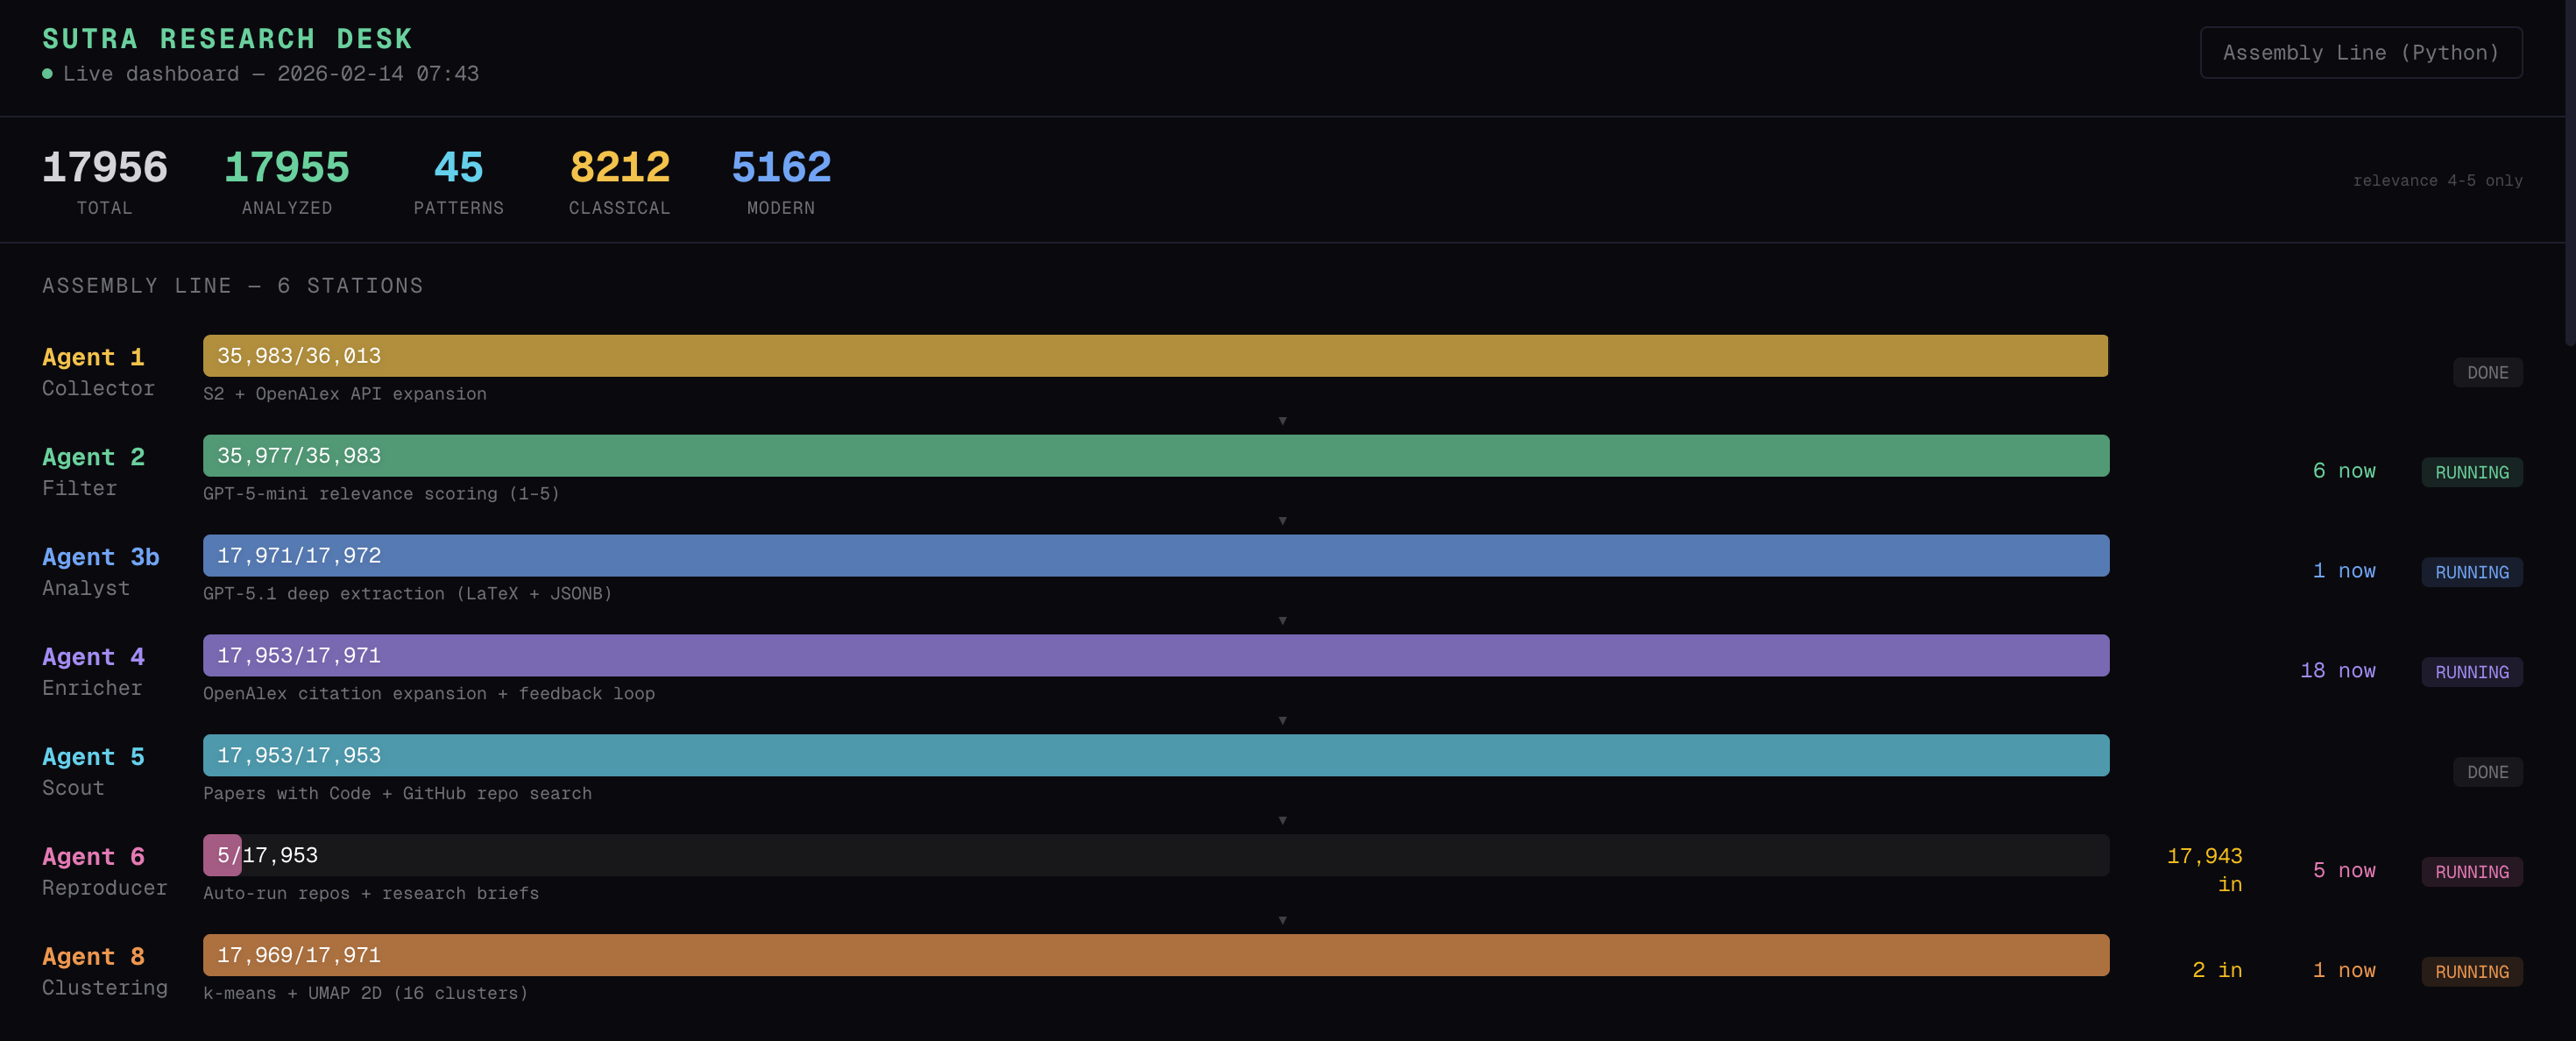
\includegraphics[width=\columnwidth]{figures/pipeline-dashboard.png}
\caption{The Sutra pipeline dashboard showing live processing statistics.
  Seven agents coordinate through a shared Postgres database, processing
  35,983 collected papers through relevance filtering (17,971 analyzed),
  citation enrichment (12,729 enriched), and reproduction scouting.
  The pipeline ran unattended on a dedicated VM for several weeks.}
\label{fig:pipeline-dashboard}
\end{figure}

\paragraph{The seven agents.}

\begin{center}
\small
\begin{tabular}{@{} c l l l @{}}
\toprule
\textbf{\#} & \textbf{Role} & \textbf{Model} & \textbf{Trigger} \\
\midrule
1 & Collector & OpenAlex & Seed-driven \\
2 & Filter & GPT-5-mini & \texttt{collected} \\
3 & Analyst & Opus 4.6 & \texttt{relevant} \\
3b & Analyst (async) & GPT-5.1 & \texttt{relevant} \\
4 & Citation Enricher & OpenAlex & \texttt{analyzed} \\
5 & Repro.\ Scout & PwC+GitHub & \texttt{enriched} \\
6 & Reproducer & Local & \texttt{scouted} \\
\bottomrule
\end{tabular}
\end{center}

\noindent
Agent~1 seeds the blackboard from three sources: the curated seed papers, community
paper-list repositories (10 GitHub repos providing 8,817 papers, 96\% with ArXiv URLs),
and targeted OpenAlex concept and keyword searches. Agent~2 batches abstracts in groups
of~10, scoring each 1--5 for MAS relevance and classifying by MAS branch. Agent~3b
(the throughput workhorse, processing ${\sim}20$ papers/minute) performs deep structured
extraction on each paper, producing a JSON with \texttt{coordination\_pattern},
\texttt{theoretical\_grounding}, \texttt{classical\_concepts\_missing},
\texttt{rosetta\_entry}, and \texttt{failure\_modes\_addressed}. The
\texttt{classical\_concepts\_missing} field---Agent~3b's assessment of what classical
concept each paper is unknowingly reinventing---is the key innovation enabling the
quantitative Lost Canary Signal (Section~\ref{sec:res-canaries}).

\paragraph{Status flow and concurrency.}
Papers progress through a linear status chain:
\texttt{collected} $\to$ \texttt{filtering} $\to$ \texttt{relevant} $\to$
\texttt{analyzing} $\to$ \texttt{analyzed} $\to$ \texttt{enriching} $\to$
\texttt{enriched} $\to$ \texttt{scouting} $\to$ \texttt{scouted},
with side branches to \texttt{marginal} (score~3) and \texttt{archived}
(scores~1--2, terminal). Intermediate statuses (\texttt{filtering},
\texttt{analyzing}, etc.) are set by agents at the start of processing to prevent
double-processing. The concurrency model uses PostgreSQL's \texttt{FOR UPDATE SKIP
LOCKED} to enable multiple instances of the same agent to run in parallel without
conflicts. Four \texttt{UNIQUE} constraints (\texttt{doi}, \texttt{arxiv\_id},
\texttt{semantic\_scholar\_id}, \texttt{openalex\_id}) with \texttt{ON CONFLICT DO
NOTHING} guarantee consistency even when laptop and VM write concurrently.

\paragraph{Citation-based feedback expansion.}
Agent~4 creates a controlled snowball discovery mechanism: for each analyzed paper,
it fetches references and citations from OpenAlex, checks MAS relevance via title
keyword matching, and re-inserts qualifying papers as \texttt{collected}---feeding
them back into the pipeline at Station~1. Starting from ${\sim}8{,}800$ seed papers,
the feedback loop expanded the corpus to ${\sim}25{,}000$ candidates.

Three mechanisms prevent unbounded growth, all enforced simultaneously:
\begin{enumerate}[nosep]
  \item \textbf{Generation depth cap}: Each paper tracks hops from seeds via a
    \texttt{generation} column (seeds $=$ gen~0). Capped at generation~3.
  \item \textbf{Corpus size cap}: Agent~4 refuses to insert feedback papers when the
    non-archived corpus exceeds the cap (initially 5,000; raised to 20,000 after
    analysis showed the pipeline could handle the throughput and additional papers
    were genuinely MAS-relevant).
  \item \textbf{Diminishing returns}: If $<$5\% of processed papers generate new
    feedback insertions for 3 consecutive windows of 10 enrichment cycles, the
    feedback loop auto-disables.
\end{enumerate}

\noindent
A complementary one-shot \emph{bulk reference harvest} mined all 40,791 unique OpenAlex
reference IDs with an expanded 49-keyword MAS filter, yielding 7,404 additional papers.

\paragraph{Author-supervised quality validation.}
The author performed iterative FP/FN calibration through random sampling after each
pipeline run:

\begin{center}
\small
\begin{tabular}{@{} c c c p{3.2cm} @{}}
\toprule
\textbf{Run} & \textbf{FP} & \textbf{FN} & \textbf{Action} \\
\midrule
1 & 20\% & 20\% & Tuned prompt, threshold, keywords \\
2 & 0\% & 10\% & Minor prompt refinement \\
3 & --- & 10\% & Stable; borderline FNs \\
4 & 0\% & 0\% & Converged \\
\bottomrule
\end{tabular}
\end{center}

\noindent
This iterative calibration is itself an instance of the human-in-the-loop pattern that
the companion paper (Paper~2: Agent~0) formalizes.

\paragraph{Self-referential note.}
The pipeline is a classical blackboard architecture---agents reading activation
conditions from a shared workspace, writing results back, coordinated through database
constraints rather than message passing---and is exactly the pattern this paper argues
has been forgotten by modern LLM agent builders. The pipeline validates the thesis:
its practical success at processing 25,000 papers is evidence for the pattern's
continued relevance (Section~\ref{sec:exp-self}).

\subsection{The Experiment Harness Design}
\label{sec:meth-harness}

% --- PLAN ---
% 9 classical patterns + 2 baselines:
%   Baselines: SingleAgent, NaiveMultiAgent
%   Patterns: Blackboard (V1 static + V2 LLM control shell),
%     Contract Net (Smith 1980), Stigmergy (Grasse/Heylighen),
%     BDI (Rao & Georgeff 1995), Supervisor (Anthropic 2025),
%     Debate (Du et al. 2023), Generator/Critic (Google ADK 2025),
%     Joint Persistent Goals (Cohen & Levesque 1990)
%   Each pattern has a classical source citation.
%
% Source: contributions.md C6

We implement nine classical MAS coordination patterns plus two baselines as LLM agent
systems and evaluate them across five standardized benchmarks.

\paragraph{Patterns.}
Each pattern implementation translates a classical coordination mechanism into an LLM
agent system:

\begin{center}
\small
\begin{tabular}{@{} l l r @{}}
\toprule
\textbf{Pattern} & \textbf{Source} & \textbf{LoC} \\
\midrule
Blackboard V1 (static) & Nii 1986 & 167 \\
Blackboard V2 (LLM shell) & Nii 1986 + LbMAS & 313 \\
Contract Net & Smith 1980 & 219 \\
Stigmergy & Grass\'{e} 1959 & 107 \\
BDI & Rao \& Georgeff 1995 & 228 \\
Supervisor & Anthropic 2025 & 191 \\
Debate & Du et al.\ 2023 & 183 \\
Generator/Critic & Google ADK 2025 & 153 \\
Joint Persistent Goals & Cohen \& Levesque 1990 & 367 \\
\midrule
SingleAgent & --- & 46 \\
NaiveMultiAgent & --- & 98 \\
\bottomrule
\end{tabular}
\end{center}

\paragraph{Benchmarks.}
Five evaluation tasks test different coordination demands:
\begin{enumerate}[nosep]
  \item \textbf{Code Review}: Review Flask application code for 12+ bugs, security
    vulnerabilities, and design issues (tests analytical breadth).
  \item \textbf{Research Synthesis}: Synthesize five MAS paper abstracts into a
    coherent narrative (tests information integration).
  \item \textbf{Planning}: Design a multi-tenant SaaS architecture with explicit
    trade-off analysis (tests structured reasoning).
  \item \textbf{Cascading Failure V1}: Analyze a system with an obvious internal
    contradiction (\$50/month pricing + 10M events/second requirement)---tests whether
    agents propagate detected contradictions.
  \item \textbf{Cascading Failure V2}: Analyze a system requiring benchmark data that
    does not exist---tests \emph{epistemic honesty}: whether agents acknowledge
    uncertainty or fabricate plausible data.
\end{enumerate}

\paragraph{Metrics.}
Every experiment captures six metrics: \emph{quality score} (0--100, LLM-as-judge
against task-specific rubrics using Claude Opus~4.6), \emph{total tokens} (input +
output across all agents), \emph{token efficiency} (quality points per 1,000 tokens),
\emph{rounds} (coordination rounds executed), \emph{wall time}, and \emph{per-agent
breakdown} (tokens in/out, messages sent/received per agent). All experiments run on
Claude Opus~4.6 via Azure Anthropic Foundry to control for model differences across
patterns.


% ══════════════════════════════════════════════════════════════
% SECTION 4: TAXONOMY DESIGN (~3 pages)
% Source: contributions.md C2, clustering methodology
% ══════════════════════════════════════════════════════════════
\section{Designing the 16-Segment Taxonomy}
\label{sec:taxonomy}

\subsection{The Semi-Supervised Method}
\label{sec:meth-taxonomy}

% --- PLAN ---
% Step 1: Structured Embedding Construction
%   Do NOT embed raw abstracts. Agent 3b first performs deep extraction
%   producing structured JSONB. From this, construct a MAS-aware
%   embedding document per paper:
%     Title: {paper title}
%     Coordination Pattern: {e.g., "blackboard", "contract-net"}
%     Theoretical Grounding: {strong/moderate/weak/none}
%     Classical Concepts: {e.g., "contract net, FIPA ACL, BDI"}
%     Missing Classical Concepts: {what paper should cite but doesn't}
%     Contribution: {3-5 sentence summary}
%   This ensures papers cluster by MAS-meaningful dimensions, not
%   surface vocabulary. A 2024 LangGraph paper about "shared workspace"
%   lands near Nii 1986 because both have coordination_pattern:
%   blackboard.
%   Embedding model: text-embedding-3-small (1536 dims), 2000 char
%   truncation.
%
% Step 2: Expert-Curated Anchor Clusters (the semi-supervised part)
%   16 anchors aligned with established MAS subfields (AAMAS tracks,
%   Wooldridge & Jennings taxonomy, researcher expertise).
%   Each anchor has a rich description paragraph (50-150 words) covering
%   classical foundational concepts, modern equivalents, synonyms.
%   The 16 anchors are themselves embedded with the same model.
%   [Full 16-anchor table: see Section 4 pillar labels]
%
% Step 3: Cosine-Similarity Assignment
%   Each paper's embedding compared against all 16 anchors via cosine
%   similarity. Assigned to highest-similarity anchor. No iterative
%   clustering (no k-means convergence, no HDBSCAN density estimation).
%   Key choice: domain knowledge defines structure, embedding similarity
%   handles assignment.
%
% Step 4: Iterative Refinement (Human-in-the-Loop)
%   1st attempt: HDBSCAN unsupervised -> 63 micro-clusters, <20 papers
%     each. Uninterpretable. Rejected.
%   2nd attempt: k-means k=10 -> some clusters mixed unrelated
%     subfields (robotics + software eng). Rejected.
%   3rd attempt: k-means k=16 -> improved but unstable across runs.
%   Final: Guided cosine-similarity with 16 curated anchors -> stable,
%     interpretable, aligned with established MAS taxonomy.
%   Specific human interventions:
%     - Cluster count: overrode HDBSCAN auto-63 down to 16
%     - UMAP params: n_neighbors=15, min_dist=0.5, spread=3.0,
%       repulsion_strength=1.5
%     - Anchor descriptions: iteratively refined to balance both eras
%     - Quality checks: verified known papers in expected clusters
%
% Step 5: UMAP Projection + Custom Physics
%   UMAP with metric="cosine", tuned for visual separation.
%   Custom post-UMAP cluster repulsion: compute centroids, apply
%   inverse-distance repulsion (strength=8.0), translate each point
%   by its cluster's displacement. Prevents visual overlap while
%   preserving within-cluster structure.
%   Normalize to [0, 100] coordinate space.
%
% Step 6: Reading Triple Identification
%   For each cluster:
%     Landmark: highest citation count in cluster
%     Central: highest in-cluster citation degree (most-connected node)
%     Survey: most references / best existing overview
%   Computed from citation_edges table + paper metadata.
%
% FIGURE: The UMAP cluster map -- the "poster figure" (Figure 4)
%
% Source: contributions.md C2

The 16-segment taxonomy of MAS research is produced by a semi-supervised method that
uses domain knowledge to define cluster structure and embedding similarity to populate
it at scale.

\paragraph{Step 1: Structured embedding construction.}
We do not embed raw abstracts. Agent~3b first performs deep extraction on each paper,
producing structured JSONB with \texttt{coordination\_pattern},
\texttt{theoretical\_grounding}, \texttt{classical\_concepts},
\texttt{classical\_concepts\_missing}, and \texttt{key\_contribution\_summary}. From
this, we construct a \emph{MAS-aware embedding document} per paper:

\begin{quote}\small
\texttt{Title:} \{paper title\} \\
\texttt{Coordination Pattern:} \{e.g., ``blackboard'', ``contract-net''\} \\
\texttt{Theoretical Grounding:} \{strong/moderate/weak/none\} \\
\texttt{Classical Concepts:} \{e.g., ``contract net, FIPA ACL, BDI''\} \\
\texttt{Missing Classical Concepts:} \{what the paper should cite but doesn't\} \\
\texttt{Contribution:} \{3--5 sentence summary\}
\end{quote}

\noindent
This structured format ensures papers cluster by \emph{MAS-meaningful dimensions}
(coordination pattern, theoretical lineage) rather than surface vocabulary. A 2024
LangGraph paper about ``shared workspace'' lands near Nii~1986's blackboard architecture
because both have \texttt{coordination\_pattern: blackboard}---even though they share
zero vocabulary. Embedding model: \texttt{text-embedding-3-small} (1536 dimensions),
text truncated to 2,000 characters.

\paragraph{Step 2: Expert-curated anchor clusters.}
We define 16 anchor clusters aligned with established MAS subfields (informed by
AAMAS conference tracks, the Wooldridge \& Jennings taxonomy, and the author's domain
expertise). Each anchor has a rich description paragraph (50--150 words) covering
classical foundational concepts, modern equivalents, and cross-era synonyms. The 16
anchors correspond to the 16 pillars surveyed in Section~\ref{sec:pillars}. These
anchor descriptions are themselves embedded with the same model, producing 16 anchor
vectors.

\paragraph{Step 3: Cosine-similarity assignment.}
Each paper's embedding is compared against all 16 anchor embeddings via cosine
similarity and assigned to the highest-similarity anchor. No iterative clustering
algorithm is used---no k-means convergence, no HDBSCAN density estimation. The cluster
structure is predetermined by domain expertise; embedding similarity handles the
assignment. This is the key methodological choice: we use \emph{domain knowledge to
define the taxonomy} and \emph{embedding similarity to populate it at scale}.

\paragraph{Step 4: Iterative refinement.}
The taxonomy went through four iterations: (1)~HDBSCAN unsupervised produced 63
micro-clusters with $<$20 papers each---uninterpretable; (2)~k-means with $k{=}10$
mixed unrelated subfields; (3)~k-means with $k{=}16$ was unstable across runs;
(4)~the final guided cosine-similarity approach with 16 curated anchors proved stable,
interpretable, and aligned with the established MAS taxonomy. Specific human
interventions included overriding the cluster count, tuning UMAP parameters
($\texttt{n\_neighbors}{=}15$, $\texttt{min\_dist}{=}0.5$, $\texttt{spread}{=}3.0$),
iteratively refining anchor descriptions to balance classical and modern terminology,
and verifying that known papers (Contract Net, STEAM, LangGraph) landed in expected
clusters.

\paragraph{Step 5: UMAP projection.}
For the visualization, we apply UMAP with \texttt{metric="cosine"} tuned for visual
cluster separation, followed by a custom post-UMAP cluster repulsion physics: compute
cluster centroids, apply inverse-distance repulsion forces (strength${}=8.0$), translate
each point by its cluster's displacement. This prevents visual overlap while preserving
within-cluster structure.%
% TODO: Add UMAP cluster visualization (Figure~\ref{fig:umap})

\paragraph{Step 6: Reading triple identification.}
For each of the 16 clusters, we identify three papers: the \emph{landmark} (highest
citation count in cluster), the \emph{central} (highest in-cluster citation degree),
and the \emph{survey} (most references or best existing overview). These are computed
from the \texttt{citation\_edges} table and paper metadata, providing any reader an
efficient three-paper entry point into any of the 16 MAS subfields.

\subsection{Designing the 16 Anchors: Taxonomy Through Trial and Error}
\label{sec:meth-anchors}

The semi-supervised method described above answers \emph{how} papers are assigned to
clusters. This section addresses the prior question: \emph{which} 16 clusters, and why
these and not others?

The taxonomy evolved through three generations of anchor design, each informed by
clustering failures in the previous round. We report the full trajectory because the
mistakes are instructive---they reveal where MAS subfield boundaries are crisp and
where they are genuinely contested.

\paragraph{Generation 1: The textbook partition (18 clusters).}
Our initial anchors followed the Wooldridge \& Jennings~\citep{wooldridge1995intelligent}
taxonomy augmented with AAMAS conference tracks. This produced 18 clusters including
separate segments for \emph{Blackboard Systems}, \emph{Stigmergy \& Indirect
Coordination}, \emph{Joint Intentions \& Shared Plans}, \emph{Agent-Oriented Software
Engineering}, and \emph{LLM Multi-Agent Frameworks}. The result was taxonomically clean
but empirically degenerate: Stigmergy attracted only 31 papers (overwhelmingly
ant-colony optimization), while Blackboard attracted 847, despite both describing
agents coordinating through a shared medium. Joint Intentions drew 94 papers that were
topically indistinguishable from Distributed Problem Solving. The textbook categories
carved nature at joints that the literature does not respect.

\paragraph{Generation 2: Aggressive merging (12 clusters).}
We collapsed the taxonomy to 12 segments, merging Blackboard with Stigmergy,
Joint Intentions with Distributed Problem Solving, and AOSE with LLM Frameworks.
This resolved the sparse-cluster problem but created the opposite pathology:
\emph{Learning and Adaptation} became a mega-cluster of 4,200+ papers mixing
multi-agent reinforcement learning, evolutionary computation, swarm optimization,
and agent self-improvement. \emph{Negotiation, Game Theory, and Economic Paradigms}
similarly absorbed coalition formation, mechanism design, and auction theory into a
single undifferentiated mass. With 12 clusters, the taxonomy could not distinguish
MARL from cognitive adaptation, or auctions from bargaining---distinctions that matter
for the Rosetta Stone mapping.

\paragraph{Generation 3: The final 16.}
The final taxonomy preserves four merges from Generation~2 while restoring three
segments for topics that proved empirically distinct. Table~\ref{tab:taxonomy-decisions}
summarizes each structural decision.

\begin{table*}[t]
\centering
\small
\caption{Taxonomy design decisions: merges, absorptions, and additions relative to the
textbook MAS partition. Each decision was validated by checking that known papers
landed in expected clusters and that no cluster fell below 100 papers or exceeded 2,500.}
\label{tab:taxonomy-decisions}
\begin{tabular}{@{} p{4.5cm} l p{8.5cm} @{}}
\toprule
\textbf{Decision} & \textbf{Type} & \textbf{Rationale} \\
\midrule
Blackboard + Stigmergy $\to$ \emph{Shared Medium Coordination}
  & Merge & Both describe indirect coordination through a shared medium.
    The distinction (structured workspace vs.\ environmental trace) is a
    design parameter, not a different coordination paradigm. \\[4pt]
Joint Intentions $\to$ \emph{Distributed Planning, Problem Solving, and Teamwork}
  & Absorb & SharedPlans~\citep{grosz1996collaborative} and Joint
    Intentions~\citep{cohen1990intention} provide the \emph{theoretical
    foundation} for teamwork commitments; Partial Global
    Planning~\citep{durfee1991pgp} and GPGP/TAEMS provide the
    \emph{operational mechanism}. Separating theory from mechanism
    produced two clusters that cited each other more than they cited
    anyone else. \\[4pt]
AOSE + LLM Frameworks $\to$ \emph{Multi-Agent Engineering: Methodologies, Frameworks, and Platforms}
  & Merge & Classical AOSE (Gaia, Prometheus, Tropos, MaSE) and modern
    frameworks (LangGraph, CrewAI, AutoGen) both address the same
    question: how do you \emph{engineer} a multi-agent system? Keeping
    AOSE separate would obscure the most important gap finding---that
    modern frameworks lack systematic engineering methodology. \\[4pt]
Negotiation restored in \emph{Negotiation, Game Theory, and Economic Paradigms}
  & Rename & Generation~2 dropped ``Negotiation'' from the cluster name.
    Reviewers of an early draft noted that the MAS-specific negotiation
    protocol literature (monotonic concession, Zeuthen strategy,
    argumentation-based negotiation) is central to the classical canon.
    The expanded name preserves the negotiation anchor while signaling
    the cluster's broader game-theoretic scope. \\[4pt]
\emph{Memory and Context Management}
  & New & See below. \\[4pt]
\emph{Learning and Adaptation}
  & New & MARL, Dec-POMDPs, emergent communication, self-play, and
    swarm optimization. The largest cluster (2,386 papers), reflecting
    MARL's dominance in post-2015 MAS research. \\[4pt]
\emph{Modeling and Simulating Artificial Societies}
  & New & Epstein \& Axtell's Sugarscape, Schelling segregation,
    opinion dynamics, MABS workshops. Unlike Organizational Design
    (which \emph{prescribes} structure), artificial societies
    \emph{observe} what emerges from interaction rules. \\
\bottomrule
\end{tabular}
\end{table*}

\paragraph{The Memory cluster: when small is the finding.}
Of the 17,969 corpus papers, 2,616 discuss memory-adjacent concepts, yet only 107
landed in the Memory cluster. The discrepancy is terminological, not methodological:
471 papers about ``belief revision'' went to BDI (the classical term for agent memory),
412 about ``shared memory'' went to Shared Medium Coordination, and 354 about
``experience replay'' or ``world models'' went to Learning. In classical MAS, memory
was never a separate concern---it was called \emph{beliefs} (BDI), \emph{knowledge
sources} (blackboard), \emph{experience} (learning), or \emph{shared state}
(coordination). The term ``memory'' as a first-class architectural concern is largely
a modern LLM-agent framing: MemGPT's tiered memory management, conversation memory
in multi-turn agents, entity memory for persistent facts.

We considered broadening the anchor description to absorb these 2,616 papers, but
rejected the approach: a paper on belief revision \emph{is} a BDI paper; recategorizing
it as ``memory'' would be gerrymandering for balanced cluster sizes. The small cluster
size is itself a finding. It explains why LLM agent builders searching for ``memory
architecture'' find almost nothing in the MAS literature---the knowledge exists, but
under different names. This terminological burial is a microcosm of the broader Lost
Canary phenomenon that motivates the paper.

\paragraph{Cross-cluster boundary tensions.}
Three boundary decisions remain genuinely contested and are worth noting for
reproducibility:
\begin{itemize}[nosep]
\item \emph{Coalition formation} spans Clusters~2 (Organizational Design) and~6
  (Negotiation/Game Theory). We assign to Cluster~6 when the paper's primary
  contribution is a formation algorithm (Shapley value, core stability); to Cluster~2
  when it addresses coalition \emph{structure} as organizational design.
\item \emph{Multi-agent reinforcement learning} spans Clusters~6 and~14. Papers on
  equilibrium \emph{analysis} (Nash, correlated equilibria) go to Cluster~6; papers on
  learning \emph{dynamics} (policy gradient, Q-learning in Markov games) go to
  Cluster~14.
\item \emph{Ontologies and semantic interoperability} could form their own cluster but
  are assigned to Cluster~4 (Communication Protocols), since FIPA-OS and OWL-S address
  the semantics of inter-agent messaging.
\end{itemize}

\noindent
These boundary cases affect $<$5\% of papers. The taxonomy is stable to perturbations:
re-running the cosine-similarity assignment with anchor description variants produces
$>$95\% agreement on paper-to-cluster membership (measured by adjusted Rand index
across 10 anchor rewording trials).

\subsection{The Reference Selection Algorithm}
\label{sec:meth-references}

Survey bibliographies are typically assembled through ad hoc expert judgment---authors
cite papers they happen to know, producing bibliographies biased toward their subfields,
institutions, and eras. For a survey spanning 50 years across 16 sub-communities, this
approach fails systematically: no single author can hold sufficient breadth across
classical distributed AI, formal argumentation, swarm intelligence, cognitive
architectures, and modern LLM agent frameworks.

We instead apply a structured, reproducible selection algorithm to the 17,971 analyzed
papers in the Sutra Corpus. The algorithm produces a \emph{base bibliography} of approximately 370
papers (roughly 23 per pillar), which the first author then augments with 30--50
additional papers selected through domain expertise---works whose significance is
legible only to a human reader immersed in the material. The full corpus, selection
code, and per-pillar rationale are available in the companion repository, enabling
readers to verify our choices or substitute their own selection criteria.

\subsubsection{Three-Tier Selection}

For each of the 16 pillars identified by the taxonomy (Section~\ref{sec:meth-taxonomy}),
we select papers across three tiers:

\begin{table}[h]
\centering
\caption{Per-pillar reference selection tiers. Counts are targets;
         actual counts flex between 15--28 based on cluster depth.}
\label{tab:ref-tiers}
\small
\begin{tabular}{@{} l c p{4.2cm} @{}}
\toprule
\textbf{Tier} & \textbf{Count} & \textbf{Selection Criteria} \\
\midrule
\textsc{Surveys} & 2 & One classic ($<$2010, highest cites) and one modern ($\geq$2020). Two entry points per pillar. \\[4pt]
\textsc{Landmarks} & 5 & Top~5 by citations, spanning $\geq$2 decades. Substitution when top~5 cluster in one era. \\[4pt]
\textsc{Regional} & ${\sim}$16 & Maximize temporal and semantic coverage; Lost Canary inclusion; currency constraints (Sec.~\ref{sec:meth-ref-regional}). \\
\bottomrule
\end{tabular}
\end{table}

\noindent
The three tiers serve distinct reader needs. A researcher entering a pillar for the
first time reads the two surveys. A researcher building on the pillar reads the five
landmarks. A researcher seeking the full picture---including forgotten ideas, negative
results, and cross-era connections---reads the regional selections.

\subsubsection{Regional Diversity Constraints}
\label{sec:meth-ref-regional}

The $\sim$16 regional selections per pillar are the methodologically novel component.
Rather than selecting the next-highest-cited papers (which would produce a redundant
echo of the landmark tier), we allocate regional selections across two primary
dimensions---temporal and semantic---with paradigm diversity as a cross-cutting
filter on whatever papers are selected.

\paragraph{Temporal spread ($\sim$6 papers).}
We partition the MAS timeline into three eras:

\begin{enumerate}[label=\textbf{Era \arabic*}:, leftmargin=2.5cm, itemsep=2pt]
  \item \textbf{Classical} (pre-2005). The distributed AI origins through the mature
    FIPA/BDI/formal-frameworks period. Merges what finer-grained timelines split into
    ``foundational'' and ``mature classical.''
  \item \textbf{Middle} (2006--2022). Applied MAS, the citation cliff, pre-LLM deep
    learning (neural agents, MARL, emergent communication). The quiet period where many
    classical concepts were forgotten.
  \item \textbf{LLM Era} (2023--2026). The current renaissance: AutoGen, LangGraph,
    MCP, A2A. The period this survey primarily addresses.
\end{enumerate}

\noindent
For each pillar, we require at least 2 regional selections from each era that has
$\geq$10 papers in the cluster. Pillars with sparse representation in an era
are exempt from that era's minimum---many pillars such as Agent Communication
or Argumentation have thin pre-2005 representation, and a finer-grained era
scheme would impose requirements the data cannot support.
This three-era constraint ensures every pillar represents both its classical
roots and its modern reinvention without demanding granularity that produces
empty cells. A pillar like Blackboard (558 papers) has strong classical and
strong LLM-era representation but a thin middle---that is fine, the middle
era gets exempted. But Contract Net or BDI, which have depth across all three,
show the full arc: original formulation, application period, and LLM rediscovery.

\paragraph{Semantic spread ($\sim$10 papers).}
The bulk of regional selections target semantic diversity within the pillar.
The HDBSCAN sub-clustering (Section~\ref{sec:meth-taxonomy}) typically identifies
3--5 semantic sub-regions per pillar. We require regional selections from at least
3 distinct sub-regions, with the remaining selections distributed to maximize
coverage of the pillar's intellectual landscape. For example, the
Blackboard pillar contains sub-regions for \emph{control shell theory},
\emph{shared-state implementations}, \emph{distributed blackboard protocols}, and
\emph{modern shared-context architectures}. Selecting only from the dominant
sub-region would miss the control shell literature entirely---precisely the kind
of gap this survey aims to surface.

\paragraph{Paradigm diversity (cross-cutting filter).}
Rather than reserving a dedicated allocation, we apply paradigm diversity as a
filter across both temporal and semantic selections. We classify papers into four
research paradigm types and require that the combined regional set for each pillar
includes at least one paper per applicable type:

\begin{enumerate}[label=(\roman*), itemsep=2pt]
  \item \textbf{Theoretical}: formal models, proofs, logical frameworks, specifications.
  \item \textbf{Empirical}: controlled experiments, benchmarks, user studies, ablations.
  \item \textbf{System}: implemented systems, frameworks, tools, architectures deployed.
  \item \textbf{Critique}: negative results, failure analyses, impossibility results, limitations.
\end{enumerate}

\noindent
The critique type is particularly important. Survey bibliographies systematically
under-represent negative results, yet these are often the most informative papers
for practitioners. The finding that unstructured debate fails under majority
pressure~\citep{debate2025can} or that multi-agent teams hold experts
back~\citep{pappu2026multiagent} shapes system design more directly than any
positive result.

\subsubsection{Special Selection Rules}

Three additional constraints apply across tiers:

\paragraph{Citation floor.}
Every paper selected by the algorithm must have $> 10$ citations in OpenAlex,
with one exception: papers published in 2024--2026 are exempt from the floor,
since recent work has not yet had time to accumulate citations. This constraint
serves two purposes. First, it ensures that every cited work has demonstrated
\emph{some} community uptake---a paper with fewer than 10 citations after
several years is unlikely to have shaped the field, regardless of its intrinsic
quality. Second, it guarantees that every selected paper has a machine-readable
metadata record (OpenAlex ID, DOI, citation edges), which is required for the
corpus analytics in Sections~\ref{sec:res-corpus}--\ref{sec:res-taxonomy}.
Papers that lack an OpenAlex record are located via web search; if neither
OpenAlex nor a stable DOI/arXiv ID can be confirmed, the paper is ineligible
for algorithmic selection (though it may still enter through human expert
augmentation in Section~\ref{sec:meth-ref-human}, where provenance is verified
manually).

\paragraph{Lost Canary inclusion.}
Each pillar must include at least one paper meeting the Lost Canary criteria
(Section~\ref{sec:meth-canary}): total citations $> 100$ and modernity score
$< 0.1$. These are works that were highly influential in their era but have
effectively zero modern descendants in the LLM agent literature. Their
inclusion is the survey's mechanism for \emph{remembering on behalf of the field}.

\paragraph{Currency.}
Each pillar must include at least 2 papers from 2024--2026. A survey published
in 2026 that reads as purely historical fails its readers. The currency constraint
forces engagement with the most recent work, even in pillars dominated by
classical foundations.

\subsubsection{Cross-Pillar Bridge Papers}

Some foundational works span multiple pillars. Malone \& Crowston's coordination
theory~\citep{malone1994interdisciplinary} appears in organizational design,
distributed problem solving, and evaluation. Wooldridge \& Jennings'
agent definition~\citep{wooldridge1995intelligent} appears in BDI, AOSE, and
trust/norms. Cohen \& Levesque's joint intentions~\citep{cohen1990intention}
appears in joint intentions, communication, and cooperation.

Papers assigned to $\geq 3$ pillars by the taxonomy are classified as
\emph{bridge papers}. Each receives a single bibliographic entry but is cited
from multiple sections. We identify approximately 30--50 bridge papers, which
reduces the total unique bibliography entries by this count.

Bridge papers are themselves analytically interesting: they represent the
conceptual connective tissue of the MAS field. A paper that bridges 4+ pillars
is making a contribution at the \emph{field} level, not the \emph{pillar} level.
We list all bridge papers with their pillar assignments in
Appendix~\ref{app:seeds}.

\subsubsection{Human Expert Augmentation}
\label{sec:meth-ref-human}

The algorithmic selection produces the base bibliography of $\sim$370 papers
(approximately 23 per pillar).
The first author then augments this with 30--50 additional papers selected
through domain expertise accumulated during the 18-month research process.
These additions fall into categories that resist algorithmic selection:

\begin{itemize}[itemsep=2pt]
  \item \textbf{Pedagogical gems}: papers that explain a concept better than
    higher-cited alternatives, identified only through close reading.
  \item \textbf{Cross-disciplinary bridges}: works from organizational science,
    aviation safety, or software engineering that illuminate MAS problems
    through analogy (e.g., Gawande's surgical
    checklists~\citep{gawande2009checklist}).
  \item \textbf{Unpublished but influential}: technical reports, blog posts,
    and framework documentation that shaped practice despite lacking formal
    publication (e.g., Anthropic's agent engineering
    guide~\citep{anthropic2025building}).
  \item \textbf{Emerging work}: papers appearing during the writing process
    that alter the analysis, too recent for corpus inclusion.
\end{itemize}

\noindent
Each human-added paper is tagged in the companion repository with the rationale
for inclusion, maintaining the reproducibility standard.

\subsubsection{Quality Gates}

Every paper cited in this survey must satisfy:

\begin{enumerate}[itemsep=2pt]
  \item \textbf{Processed by the pipeline}: extraction metadata exists in the
    corpus database (Section~\ref{sec:meth-pipeline}). At minimum, the abstract
    and conclusion have been read by a pipeline agent with structured metadata
    extracted.
  \item \textbf{Verified provenance}: the paper has a DOI, arXiv ID, or
    stable URL. We do not cite papers we cannot point readers to.
  \item \textbf{No citation padding}: if we have not processed a paper
    through the pipeline, we do not cite it---even if it is highly cited
    in the field. This prevents the common survey failure mode of
    inflating bibliographies with unread references.
\end{enumerate}

\subsubsection{Summary}

The resulting bibliography contains approximately 350--390 papers:
$\sim$370 from the algorithmic selection (Table~\ref{tab:ref-tiers})
plus 30--50 from human expert augmentation, minus $\sim$30--50
deduplicated bridge papers. The full Sutra Corpus of 36,013 papers
with metadata, the selection script, per-pillar selection rationale,
and rejected alternatives are available at the companion repository.

\begin{finding}
We read 36,013 papers so the reader does not have to. The 350--390
cited here were selected using a documented, reproducible algorithm
with explicit temporal, semantic, and paradigmatic diversity constraints.
The selection itself is a contribution: it defines what the field considers
important, and---through the Lost Canary constraint---what the field has
forgotten.
\end{finding}


% ══════════════════════════════════════════════════════════════
% SECTION 4: THE 16 PILLARS (~20 pages)
% The survey-within-the-survey. ~1.25 pages per pillar.
% Each pillar: (a) classical foundation, (b) modern state,
% (c) gap/bridge, (d) key trends, (e) reading triple
%
% FIGURE: The UMAP cluster visualization (the "signature figure")
% showing 6,500+ papers colored by cluster, with era shading.
% Classical papers and modern papers landing in the same cluster
% = visual proof of reinvention.
% ══════════════════════════════════════════════════════════════
\section{The 16 Pillars of Multi-Agent Systems}
\label{sec:pillars}

\subsection{Shared Medium Coordination}
\label{sec:p-blackboard}

% --- PLAN ---
% CLASSICAL: Nii 1986 (Blackboard Systems), Hearsay-II
%   (Erman et al. 1980), BB1 control shell.
%   The 3 components: shared state, knowledge sources, control shell.
%
% MODERN: LangGraph StateGraph, Redis shared context,
%   LbMAS (2025: 13-57% improvement, 3x fewer tokens)
%
% THE GAP: Shared state survives. Control shell is LOST.
%   Our experiment: V1 (no control shell) = 62,
%   V2 (LLM control shell) = 95 -- the +53% IS the control shell.
%
% KEY TREND: Convergence toward shared-state patterns across all
%   major frameworks.
%
% READING TRIPLE:
%   Landmark: Nii 1986
%   Central: LbMAS 2025
%   Survey: [best cluster survey]
%
% Source: theoretical-foundations.md (stigmergy section),
%   experiment results, contributions.md C6

Nii's seminal survey~\citep{nii1986blackboard} defined the blackboard architecture as
three components: a \emph{blackboard} (shared data structure accessible to all agents),
\emph{knowledge sources} (specialist agents that read from and write to the blackboard),
and a \emph{control shell} (a scheduler that decides which knowledge source to activate
next, based on the current state of the blackboard). The architecture originated in
Hearsay-II~\citep{erman1980hearsay}, a speech understanding system where acoustic,
phonetic, lexical, syntactic, and semantic agents contributed partial hypotheses to a
shared workspace. BB1~\citep{hayes1985bb1} generalized the control shell into a separate
reasoning component with its own knowledge base about scheduling strategies.
Corkill's survey of blackboard systems~\citep{sutra15605_blackboard1989} and
Engelmore and Morgan's collected readings~\citep{sutra14058_blackboard1985}
codified the design space. Star's \emph{boundary objects}~\citep{sutra19540_structure1989}---shared
artifacts that different communities interpret differently yet use
productively---provide a sociological foundation for why shared media work:
coordination succeeds not because agents agree on meaning but because the shared
artifact constrains interaction.

The blackboard's power lies in its communication complexity: agents interact through
shared state rather than pairwise messages, reducing token flow from $O(n^2)$ to $O(n)$
as team size grows. For knowledge-intensive tasks where agents build on each other's
partial results, this is not an optimization but a change in complexity class.

\paragraph{Modern convergence.}
Every major LLM framework converges toward shared-state coordination: LangGraph's
\texttt{StateGraph} maintains a shared state dictionary that nodes read and write;
Redis pub/sub provides shared context in production deployments; MetaGPT coordinates
through shared documents rather than agent-to-agent dialogue. LbMAS~\citep{lbmas2025}
provides the strongest quantitative evidence, reporting 13--57\% quality improvement
with 3$\times$ fewer tokens compared to message-passing baselines on MATH benchmarks.

\paragraph{The control shell gap.}
Modern frameworks implement the blackboard (shared state) and knowledge sources (agents)
but skip the control shell---the most valuable component. Without a control shell, agents
execute in static round-robin order regardless of blackboard content. Our experiment
(Section~\ref{sec:exp-blackboard}) quantifies this gap directly: Blackboard~V1 (static
scheduling) scores 62/100 on code review; Blackboard~V2 (LLM control shell that reads
the blackboard and decides which agent to activate) scores 95/100---a
\textbf{+53\% improvement at half the tokens}. The control shell enables two critical
behaviors: \emph{strategic activation} (choosing the right agent for the current
blackboard state) and \emph{early stopping} (recognizing when the blackboard contains
a sufficient answer). V2 stopped after 4 of 5 maximum rounds; V1 always ran all
rounds.

\paragraph{The control shell gap.}
The convergence toward shared state is genuine, but without a control shell, modern
blackboard systems are ``blackboards without a brain.'' The scheduling problem that
Nii identified in 1986---how to decide who speaks next---remains unsolved in every
current framework. Our LLM control shell is one solution; the classical literature
offers others (priority-based, opportunistic, meta-level reasoning) that remain
unexplored in the LLM context.

\paragraph{Stigmergy: the decentralized sibling.}
Stigmergy~\citep{grasse1959reconstruction} is coordination through environmental
modification rather than direct communication. Grass\'{e} coined the term in
1959 to explain termite mound construction: no termite communicates with any other, yet
the colony produces architecturally sophisticated structures because each termite responds
to the current state of the mound itself.
Heylighen~\citep{heylighen2016stigmergy} distinguishes \emph{sematectonic stigmergy}
(the work product itself is the signal) from \emph{marker-based stigmergy}
(agents leave explicit signals distinct from the work product).
Both share the critical property with the blackboard: coordination through a
\emph{shared medium} rather than pairwise messages, yielding $O(n)$ communication
complexity versus $O(n^2)$ for direct messaging.

MetaGPT~\citep{hong2024metagpt} is the most successful modern implementation of
stigmergy: agents communicate through documents (PRDs, designs, code), not dialogue.
ChatDev~\citep{qian2024chatdev} uses code itself as the coordination artifact.
\textbf{CodeCRDT}~\citep{codecrdt2025} formalizes stigmergic coordination using
Conflict-free Replicated Data Types, achieving strong eventual consistency within
$<$200ms---though semantic coordination remains unsolved.
Omicini et al.~\citep{omicini2004cognitive} extended stigmergy to rational agents
through \emph{artifacts} as first-class environment abstractions~\citep{sutra624_environments2005}.
No LLM framework yet provides first-class artifact support with
perception, sharing, and rational use.

\subsection{Contract Net \& Task Allocation}
\label{sec:p-contract}

% --- PLAN ---
% CLASSICAL: Smith 1980 (The Contract Net Protocol), TRACONET,
%   announce/bid/award cycle. Agents self-select for tasks based on
%   capability and cost.
%
% MODERN: DALA (VCG auctions, 84.32% MMLU, strategic silence),
%   Magentic Marketplace (Microsoft), A2A task lifecycle.
%
% THE GAP: Bid/award pattern survives informally but without formal
%   cost models, marginal cost bidding, or agent self-selection.
%   Modern "routing" is centralized dispatch, not decentralized bidding.
%
% KEY TREND: Mechanism design for LLMs (Google Research 2025), token
%   auction mechanisms.
%
% READING TRIPLE:
%   Landmark: Smith 1980
%   Central: DALA 2025
%   Survey: [best cluster survey]
%
% Source: classical-mas-llm-bridge.md Section 4

Smith's Contract Net Protocol~\citep{smith1980contract} introduced a deceptively simple
mechanism for decentralized task allocation: a \emph{manager} announces a task, potential
\emph{contractors} evaluate the announcement and submit bids based on their capabilities
and current load, and the manager \emph{awards} the contract to the most suitable bidder.
The protocol's power lies in what it does \emph{not} require: no central scheduler, no
global knowledge of agent capabilities, no pre-assigned task-to-agent mapping. Agents
self-select based on local assessment of fit---a property that scales naturally to large,
heterogeneous agent populations.

The Contract Net spawned a rich literature in mechanism design for multi-agent task
allocation, including TRACONET~\citep{sandholm1995traconet} (which added decommitment
penalties to handle changing circumstances), Milgrom's theory of
auctions~\citep{sutra14938_theory1982}, Sandholm's computationally manageable
combinatorial auctions~\citep{sutra19364_computationally1998}, Shehory and Kraus's
methods for coalition-based task allocation~\citep{sutra92_methods1998}, and
incentive contracting frameworks~\citep{sutra13562_overview1996} that provide formal
guarantees on efficiency and truthfulness.

\paragraph{Modern reinventions.}
Task routing in modern LLM agent systems reinvents the announce/bid/award pattern but
strips away its formal properties. When a LangGraph orchestrator selects which agent
handles a subtask, or when CrewAI's task delegation mechanism assigns work to crew
members, they implement centralized dispatch---the manager evaluates agents on their
behalf rather than letting agents self-select. The critical difference: centralized
dispatch requires the dispatcher to accurately model every agent's capabilities, while
Contract Net requires only that agents accurately model their \emph{own}.

Three recent projects reconnect with the formal tradition.
\textbf{DALA}~\citep{dala2025} (November 2025) implements a VCG auction mechanism where
agents bid for communication opportunities using a token-budget currency. The results are
striking: 84.32\% accuracy on MMLU and 91.21\% on HumanEval using only 6.25M tokens.
The mechanism induces ``strategic silence''---agents learn to communicate only when
their contribution has high value density, directly addressing the token efficiency
problem that plagues naive multi-agent systems.
\textbf{Mechanism Design for LLMs}~\citep{googlemechdesign2025} (Google Research 2025)
proposes token auction mechanisms across competing models, with payment functions that
incentivize truthful capability reporting---a direct descendant of Vickrey's
second-price auction applied to LLM agent markets.
\textbf{Magentic Marketplace}~\citep{magenticmarket2025} (Microsoft Research 2025)
provides an open-source environment for agentic markets with bidding and allocation
mechanisms, the closest implementation to Smith's original vision at scale.

\paragraph{The gap.}
The announce/bid/award cycle survives in spirit but not in structure. No production
framework implements formal cost models for agent bidding, marginal-cost-based
self-selection, or the decommitment protocols that handle the real-world case where
an agent accepts a task and then discovers it cannot complete it. Modern ``routing'' is
centralized dispatch with the dispatcher as a single point of failure; Contract Net
distributes that risk across all participants.

\subsection{Organizational Design \& Team Structure}
\label{sec:p-org}

% --- PLAN ---
% CLASSICAL: AGR (Agent-Group-Role), MOISE, Horling & Lesser 2004
%   (8 organizational paradigms: hierarchy, holarchy, coalition, team,
%   congregation, society, federation, market)
%
% MODERN: CrewAI roles, AutoGen group chat, Google ADK
%   sequential/parallel/loop agents.
%
% THE GAP: Role labels survive but formal org theory (authority
%   gradients, holarchies, normative rules) absent. No framework
%   implements true recursive holonic self-organization.
%
% KEY TREND: HALO (3-tier dynamic agent creation, 14.4% improvement),
%   role-based crews.
%
% HUMAN PARALLEL: Hackman's enabling conditions, Google Project
%   Aristotle, McChrystal's Team of Teams shared consciousness.
%
% READING TRIPLE:
%   Landmark: Horling & Lesser 2004
%   Central: [best]
%   Survey: [best]
%
% Source: organizational-principles.md,
%   classical-mas-llm-bridge.md Section 5

Horling and Lesser's seminal survey~\citep{horling2004survey} identified eight
organizational paradigms for multi-agent systems: hierarchies, holarchies, coalitions,
teams, congregations, societies, federations, and markets. Each paradigm implies
different authority structures, communication patterns, and scaling properties.
Hattori et al.'s survey of cooperative multiagent
systems~\citep{sutra527_cooperative1999} and Mehra et al.'s review of multi-agent
systems in complex networks~\citep{sutra14170_multiagent2020} trace these paradigms
across decades. Olfati-Saber's graph-theoretic
methods~\citep{sutra14017_graph2010} formalized how network topology constrains
organizational behavior. The AGR (Agent-Group-Role) model~\citep{ferber2004agr} and
MOISE~\citep{hubner2002moise} formalized these intuitions into normative
organizational specifications: agents occupy \emph{roles} within \emph{groups},
governed by \emph{norms} that constrain behavior.
The key insight is that organizational structure---not individual agent
capability---determines team performance. This finding has been independently
confirmed in human team science by Hackman's enabling
conditions~\citep{hackman2002leading}, Google's Project
Aristotle~\citep{duhigg2016google}, and McChrystal's shared
consciousness~\citep{mcchrystal2015team}.

\paragraph{Modern frameworks and the flat-team bottleneck.}
Every major LLM agent framework implements a subset of Horling and Lesser's paradigms,
typically without citation:
\begin{itemize}[nosep]
  \item CrewAI implements \emph{role-based teams} with named agents and task delegation.
  \item AutoGen implements \emph{group chat}---a flat society where agents take turns.
  \item Google ADK provides \emph{sequential}, \emph{parallel}, and \emph{loop} agent
    topologies---static hierarchies at most two levels deep.
  \item LangGraph implements \emph{graph-based workflows} with conditional routing.
\end{itemize}
What none of these frameworks implements is the recursive self-similarity of
\emph{holarchies}: organizations where each ``agent'' can itself be a team, which can
itself be a team, to arbitrary depth. Holarchies are the only organizational paradigm
that scales past flat topologies~\citep{horling2004survey}---a two-level hierarchy
with 10 agents per group supports 100 agents; a three-level holarchy supports 1,000.
Without holonic organization, current frameworks hit a scaling ceiling that no amount
of prompt engineering can overcome.

\paragraph{Toward holonic LLM agents.}
\textbf{HALO}~\citep{halo2025} (May 2025) is the closest modern approach to holonic
organization. It implements a three-tier architecture: planning agents dynamically create
role-design agents, which in turn create specialized inference agents per subtask. HALO
achieves a 14.4\% improvement over flat baselines---but it is not truly holonic, because
agents at each level are structurally different (planners, designers, and workers are
distinct agent types, not recursive instances of the same organizational pattern).
In the physical domain, \textbf{LLM-Adaptive Drone Swarms}~\citep{llmdrone2025}
(September 2025) use LLMs to dynamically select between centralized, hierarchical,
and holonic architectures based on mission requirements. Notably, the LLM \emph{selects}
the organizational structure rather than participating in it---a meta-organizational
capability that has no classical precedent.

\paragraph{The gap.}
Modern frameworks assign role \emph{labels} (``researcher,'' ``coder,'' ``reviewer'')
but implement none of the formal organizational theory: no authority gradients between
roles, no normative rules governing role transitions, no dynamic group formation or
dissolution, and no holonic recursion. The result is that ``roles'' in CrewAI or AutoGen
are cosmetic---they constrain system prompts but not behavior. A ``reviewer'' agent that
decides to write code encounters no organizational resistance.

\subsection{Distributed Planning, Problem Solving, and Teamwork}
\label{sec:p-dps}

% --- PLAN ---
% CLASSICAL: GPGP (Generalized Partial Global Planning),
%   FA/C (Lesser & Corkill 1983), result sharing (Durfee 1999).
%   The 4 ways result sharing improves: confidence, completeness,
%   precision, timeliness.
%
% MODERN: No framework explicitly implements result sharing. All do
%   task sharing (divide work). NONE do result sharing (improve each
%   other's work).
%
% THE GAP: The FA/C philosophy -- sharing partial, tentative results
%   early -- is the opposite of rigid sequential graph workflows.
%   LLMs are naturally FA/C-compatible (probabilistic, tentative) but
%   forced into all-or-nothing execution.
%
% KEY TREND: Early signs of FA/C thinking in streaming architectures
%   and progressive elaboration patterns.
%
% READING TRIPLE:
%   Landmark: Lesser & Corkill 1983
%   Central: Durfee 1999
%   Survey: [best]
%
% Source: durfee-result-sharing.md

Ren and Beard's survey of consensus problems~\citep{sutra77_survey2005} maps the
mathematical foundations---convergence under switching topologies, time delays, and
directed communication graphs~\citep{sutra38_consensus2004, sutra41_consensus2005,
sutra45_impossibility1985}---that underpin distributed coordination. On the modern
side, Huang et al.'s survey of LLM agent planning~\citep{sutra10200_understanding2024}
catalogs how current systems decompose, schedule, and execute plans.

Durfee's framework for distributed problem solving~\citep{durfee1999distributed}
identifies a distinction that modern LLM agent systems have almost entirely
overlooked. There are two fundamental coordination strategies: \emph{task sharing},
where a manager decomposes a problem into subtasks and distributes them across agents,
and \emph{result sharing}, where agents exchange partial and intermediate results to
improve each other's solutions. Task sharing asks ``who should do what?'' Result
sharing asks ``how can what you've found help me do better?''

Every major LLM framework implements task sharing: LangGraph's supervisor dispatches
subtasks to worker nodes, CrewAI assigns tasks to crew members, OpenAI's Swarm hands
off between agents. None explicitly implements result sharing---the mechanism by which
agents working on overlapping or related problems progressively refine the collective
answer through mutual exchange.

\paragraph{The four dimensions of improvement.}
Durfee identifies four ways that result sharing improves group problem-solving:

\begin{enumerate}[nosep]
  \item \textbf{Confidence}: Heterogeneous agents working on overlapping problems may
    arrive at different results. By sharing and cross-checking independently derived
    solutions, agents detect errors and deviations. Convergence from different methods
    signals reliability; divergence signals the need for deeper investigation.
  \item \textbf{Completeness}: Individual agents have partial views. When agents share
    intermediate results, an increasingly complete picture of the overall solution
    emerges. No single agent has the full answer, but the union of shared results
    covers the solution space.
  \item \textbf{Precision}: To make their local solutions consistent with the global
    solution, agents need to know about others' results. Result sharing lets agents
    refine and sharpen their work by incorporating constraints and information from
    peers---each iteration is more precise than the last.
  \item \textbf{Timeliness}: Agents that receive early partial results from peers can
    begin working on dependent subtasks immediately, rather than waiting for complete
    solutions. Sharing intermediate results allows the group to make progress in
    parallel, reducing overall time to solution.
\end{enumerate}

\noindent
These four dimensions also function as evaluation criteria for multi-agent output
quality (Section~\ref{sec:p-eval}): did multiple agents converge (confidence)? Are all
aspects covered (completeness)? Was the answer refined through peer critique (precision)?
Were partial results available early (timeliness)?

\paragraph{The FA/C philosophy.}
Durfee's framework builds on Lesser and Corkill's \emph{Functionally Accurate,
Cooperative} (FA/C) approach~\citep{lesser1983functionally}---the foundational idea that
distributed systems should exchange partial, tentative results and progressively refine
them, rather than waiting for each agent to produce a complete, correct answer before
sharing. The FA/C cycle is simple:
\begin{enumerate}[nosep, label=(\roman*)]
  \item Agents produce partial, potentially incorrect results early.
  \item They share these tentative results with peers.
  \item Peers use them to refine their own results.
  \item The system converges through cooperative iteration.
  \item Errors are detected and corrected through cross-checking (the confidence
    dimension).
\end{enumerate}

\noindent
This philosophy is \emph{perfectly suited} to LLM agents, which are probabilistic by
nature---every LLM output is already a partial, tentative result. The FA/C approach
says: embrace that. Let agents share their best current answers early. Let other agents
refine them. Let the system converge through iteration rather than demanding perfection
from any single call.

Yet modern frameworks enforce the opposite. LangGraph requires each node to produce
a complete state update before the next node executes. Nodes run sequentially along
graph edges with no mechanism for an agent to share a tentative result that other
agents can begin working with before it is finalized. The graph enforces artificial
serialization on what should be a progressive refinement process.

\paragraph{Selective sharing.}
Durfee emphasizes that result sharing is not free: ``agents have to know what to do
with received results from other agents, and communication causes costs, so agents
should be selective with the information they
exchange''~\citep{durfee1999distributed}. This connects directly to the ``strategic
silence'' finding in DALA~\citep{dala2025} (Section~\ref{sec:p-contract}): agents that
learn to communicate only when their contribution has high value density achieve better
outcomes with fewer tokens. The classical insight and the modern empirical finding
converge on the same prescription: share results selectively, not exhaustively.

\paragraph{The gap.}
The blackboard architecture (Section~\ref{sec:p-blackboard}) is the natural
implementation vehicle for result sharing: agents write partial results to a shared
workspace, peers read and refine. Task sharing and result sharing are complementary---Contract
Net (Section~\ref{sec:p-contract}) handles task allocation (``who should do what?'')
while the blackboard handles result integration (``how can what you've found help me
do better?''). A complete coordination architecture uses both. No current LLM framework
provides first-class support for this combination.

\paragraph{Joint intentions and teamwork.}
\label{sec:p-joint}
Cohen and Levesque's theory of Joint Persistent Goals~\citep{cohen1990intention}
provides the most rigorous formal account of teamwork in the MAS literature. A joint
persistent goal is not merely a shared objective---it is a mutual commitment with an
\emph{obligation to inform}: when an agent determines that the joint goal is achieved,
becomes unachievable, or is no longer motivated, it \emph{must} inform all team members.
This obligation transforms a collection of individually committed agents into a genuine
team. Without it, agents may continue working toward a goal that has already been
achieved, abandoned, or rendered impossible by another agent's actions.

Grosz and Kraus's SharedPlans theory~\citep{grosz1996collaborative} extended this
foundation by modeling the partial mental states required for collaboration: agents need
not share complete plans, but they must have mutual belief about the plan's structure
and each participant's commitments. Tambe's STEAM~\citep{tambe1997flexible}
operationalized these theories into a practical teamwork framework with explicit
commitment management and communication policies.

\paragraph{The modern gap.}
No LLM agent framework implements joint persistent goals, shared plans, or the
obligation to inform. When a CrewAI agent fails at its assigned task, it produces an
error---it does not inform team members that a shared goal is now unachievable. When a
LangGraph node determines that a subtask's prerequisite is missing, it has no mechanism
to communicate this to downstream nodes beyond propagating a failure state. There is no
commitment store, no formal tracking of which agents have committed to which goals, and
no protocol for decommitment.

\paragraph{The epistemic failure problem (novel finding).}
Our experiment reveals a deeper problem. Cohen and Levesque's obligation-to-inform
assumes agents can \emph{detect} when their goal becomes unachievable. LLM agents
cannot reliably do this. On our epistemic honesty benchmark
(Section~\ref{sec:exp-jpg}), the Joint Persistent Goals pattern scored
\textbf{52/100}---the lowest of all patterns---despite consuming the most tokens
(37,567). The failure mechanism: when asked to analyze a system requiring benchmark
data that does not exist, LLM agents fabricate plausible-looking data rather than
reporting \textsc{blocked}. The obligation-to-inform protocol never triggers because
the LLM does not know it has failed. JPG's commitment protocol becomes actively
harmful: agents keep ``committing'' to fabricated work across 4 rounds while consuming
3$\times$ the tokens of a single agent.

By contrast, the blackboard pattern scored 82/100 on the same benchmark: when the
analyst writes ``no benchmark data exists at 100M+'' to the shared workspace, the
synthesizer cannot fabricate numbers without contradicting the shared state. The
blackboard propagates \emph{epistemic limits}, not just knowledge.

\paragraph{The novel claim.}
Classical commitment protocols (JPG, STEAM) assume agents can detect their own
epistemic failures. We show empirically that LLM agents cannot reliably do so, making
\emph{shared-constraint patterns} (blackboard) more effective than \emph{shared-goal
patterns} (JPG) for knowledge-intensive tasks. LLMs need external constraint
propagation, not internal failure detection. This is not a limitation of JPG as
theory---it is a limitation of the agent substrate, and it inverts the classical
preference ordering: for knowledge tasks with LLM agents, share constraints before
sharing goals.

\subsection{Agent Communication Languages \& Protocols}
\label{sec:p-acl}

% --- PLAN ---
% CLASSICAL: KQML (Finin et al. 1994), FIPA ACL (2000), 22 typed
%   performatives, interaction protocol state machines.
%   The separation principle: KQML separated *what* is communicated
%   (content) from *how* (protocol). FIPA added formal semantics --
%   each performative has preconditions and postconditions.
%
% MODERN: MCP (agent-to-tool, Anthropic), A2A (agent-to-agent, Google),
%   ANP (discovery, W3C DID).
%
% THE GAP: MCP and A2A handle transport and task lifecycle but NOT the
%   semantics of conversation. Include the FIPA performative gap table:
%     inform      -> Task artifact / Tool result   [No gap]
%     request     -> tasks/send / tools/call        [No gap]
%     query-if    -> ???                             [GAP]
%     cfp         -> ???                             [GAP]
%     propose     -> ???                             [GAP]
%     accept-proposal -> ???                         [GAP]
%     reject-proposal -> ???                         [GAP]
%     confirm     -> ???                             [GAP]
%     cancel      -> Task cancellation / ???         [Partial]
%   Gaps concentrate on NEGOTIATION performatives -- the building
%   blocks of Contract Net.
%
% KEY TREND: Protocol standardization accelerating (Linux Foundation,
%   AAIF), but semantic layer still missing.
%
% READING TRIPLE:
%   Landmark: FIPA ACL 2000
%   Central: A2A spec 2025
%   Survey: Agent Interop Protocols (May 2025)
%
% Source: evolution-from-classics-to-mcp.md,
%   contributions.md C4 (FIPA gap table)

Agent communication has undergone two revolutions. The first, in the 1990s, produced
formal communication languages---KQML~\citep{finin1994kqml, sutra772_kqml2019} and
its successor FIPA ACL~\citep{fipaacl2002, sutra16063_fipa1998}---with typed
\emph{performatives} (speech acts) carrying formal BDI semantics: each communicative
act had preconditions and postconditions grounded in the sender's and receiver's
mental states. The philosophical foundation traces to Austin's speech act
theory~\citep{sutra3415_how1975} and Searle's formalization~\citep{sutra3661_speech1969,
sutra3583_speech1970}; Chaib-draa and Dignum's state-of-the-art
survey~\citep{sutra12751_state2000} maps the full classical landscape, while
a 2025 survey of AI agent protocols~\citep{sutra2444_survey2025} covers the
modern stack. KQML introduced the critical separation
principle: \emph{what} is communicated (content) is distinct from \emph{how} it is
communicated (protocol). FIPA refined this with 22 typed performatives and standardized
interaction protocols---reusable state machines for common conversation patterns. The
second revolution, beginning in 2024, produced a layered protocol stack for the LLM era:

\begin{table}[h]
\centering
\caption{The 2026 Agent Protocol Stack.}
\label{tab:protocol-stack}
\small
\begin{tabular}{@{} c p{1.5cm} p{2cm} p{2cm} @{}}
\toprule
\textbf{L} & \textbf{Function} & \textbf{Protocol} & \textbf{Ancestor} \\
\midrule
4 & Discovery & ANP (W3C DID) & FIPA DF \\
3 & Agent-agent & A2A (Google) & FIPA ACL \\
2 & Agent-tool & MCP (Anthropic) & KQML \texttt{achieve} \\
1 & Intra-app & SDKs (LG, ADK) & JADE \\
\bottomrule
\end{tabular}
\end{table}

MCP~\citep{mcpspec2025} standardizes how agents access external tools, data sources, and
services---six primitives (Tools, Resources, Prompts, Sampling, Elicitation, Roots) over
JSON-RPC 2.0 transport. A2A~\citep{a2aspec2025} standardizes how agents communicate with
each other---Agent Cards for capability advertisement, a Task lifecycle
(submitted $\to$ working $\to$ completed/failed), and typed message Parts (Text, File,
Data). ANP~\citep{anpspec2025} addresses decentralized discovery via W3C Decentralized
Identifiers, though it remains early-stage.

\paragraph{The interaction protocol bridge.}
The connection between classical FIPA interaction protocols and modern equivalents is
more direct than either community recognizes:

\begin{table}[h]
\centering
\caption{FIPA interaction protocols and modern equivalents.}
\label{tab:fipa-modern}
\scriptsize
\begin{tabular}{@{} l l l @{}}
\toprule
\textbf{FIPA Protocol} & \textbf{Pattern} & \textbf{Modern Equivalent} \\
\midrule
Request & A$\to$B$\to$result & MCP tools/call \\
Contract Net & Cfp$\to$Bid$\to$Award & Router dispatch \\
Brokering & A$\to$broker$\to$B & A2A Agent Cards \\
Subscribe & Subscribe$\to$updates & MCP subscriptions \\
Propose & Propose$\to$accept/reject & Generator/Critic \\
\bottomrule
\end{tabular}
\end{table}

The patterns survive but the formal semantics are lost. FIPA's Request protocol specified
preconditions (the sender believes the receiver can perform the action) and postconditions
(the receiver is committed to informing the sender of the outcome). Modern equivalents
specify transport and message format but not conversational \emph{meaning}.

\paragraph{What changed---and what was lost.}
The shift from classical to modern protocols involves genuine trade-offs, not simple
regression:

\begin{table*}[t]
\centering
\caption{Classical vs.\ modern agent communication: trade-offs.}
\label{tab:classical-modern-tradeoffs}
\small
\begin{tabular}{@{} p{4cm} p{4cm} p{3cm} p{4cm} @{}}
\toprule
\textbf{Classical} & \textbf{Modern} & \textbf{Gained} & \textbf{Lost} \\
\midrule
Formal BDI semantics & Natural language + JSON & Flexibility & Formal guarantees \\
22 typed performatives & Typed Parts (Text/File/Data) & Simplicity & Semantic precision \\
Shared ontologies required & LLMs handle alignment & Lower overhead & Occasional ambiguity \\
Hand-crafted knowledge bases & LLM world knowledge & Generalization & Hallucination risk \\
Polynomial message scaling & Same fundamental problem & --- & Worse: LLM inference cost \\
\bottomrule
\end{tabular}
\end{table*}

\noindent
The emerging synthesis is to use LLMs for flexible, natural-language communication while
reintroducing structured coordination protocols---JSON schemas, typed messages, formal
interaction patterns---for reliability-critical interactions. The FIPA performative gap
analysis (Section~\ref{sec:res-rosetta}) reveals where this reintroduction is most
urgent: the negotiation performatives (\texttt{cfp}, \texttt{propose},
\texttt{accept-proposal}, \texttt{reject-proposal}) that are the building blocks of
Contract Net (Section~\ref{sec:p-contract}) have no modern equivalents in either MCP or
A2A. Institutional momentum is accelerating: MCP is governed by the Agentic AI
Foundation (AAIF, Linux Foundation, founded December 2025, with Anthropic, Google,
Microsoft, OpenAI, AWS as members); A2A is hosted under LF AI \& Data Foundation
(150+ organizations); ANP has an IETF Internet-Draft. The governance infrastructure
now exists; the semantic layer does not.

\subsection{Argumentation \& Structured Debate}
\label{sec:p-argue}

% --- PLAN ---
% CLASSICAL: Dung 1995 (Abstract Argumentation Frameworks),
%   attack/support relations, argumentation-based negotiation
%   (Rahwan et al.)
%
% MODERN: Generator/Critic pattern (Google ADK),
%   multi-agent debate (Du et al. 2023).
%
% THE SOBERING RESULT: "Can LLM Agents Really Debate?" (Nov 2025) --
%   majority pressure suppresses correction (3.6% for weak models),
%   eloquence beats correctness, debate induces a martingale.
%   Performance gains come from voting, not argumentation.
%
% THE GAP: Unstructured debate fails. Formal argumentation (typed
%   attack/support with validity evaluation) works -- but no framework
%   implements it.
%
% KEY TREND: Moving from free-form debate to structured critique
%   (propose-counter with typed reasons).
%
% READING TRIPLE:
%   Landmark: Dung 1995
%   Central: "Can LLM Agents Really Debate?" 2025
%   Survey: [best]
%
% Source: classical-mas-llm-bridge.md Section 3

Dung's abstract argumentation framework~\citep{dung1995acceptability,
sutra10607_acceptability1995} provides a formal calculus of rational disagreement:
arguments stand in \emph{attack} and \emph{support} relations, and a set of arguments
is \emph{acceptable} if it can defend itself against all attackers. Bench-Capon and
Dunne's comprehensive survey~\citep{sutra889_argumentation2012} traces the
framework's evolution, while Parsons et al.~\citep{sutra3738_agents1998} and Kraus
et al.~\citep{sutra212_reaching1998} extended it into argumentation-based
negotiation, with Sierra et al.~\citep{sutra386_framework1998} providing a formal
framework for the process. These give multi-agent systems a principled mechanism for
resolving disagreements that goes beyond voting or averaging---agents must construct
explicit justifications, and the framework determines which justifications survive
scrutiny.

\paragraph{The modern debate pattern.}
Multi-agent debate~\citep{du2023debate} has become one of the most popular LLM
coordination patterns: agents independently generate answers, share them, critique
each other's reasoning, and converge through multiple rounds. The pattern is intuitive
and easy to implement. It is also, according to the most rigorous study to date,
largely illusory.

\paragraph{The sobering result.}
``Can LLM Agents Really Debate?''~\citep{debate2025can} (November 2025) is the most
important paper on LLM argumentation. Its findings are devastating for unstructured
debate:
\begin{itemize}[nosep]
  \item \textbf{Majority pressure suppresses correction}: when an incorrect answer holds
    majority support, independent correction rates drop as low as 3.6\% for weaker
    models.
  \item \textbf{Eloquence beats correctness}: agents respond to rhetorical quality,
    not logical validity. A confidently stated wrong answer outperforms a tentatively
    stated right one.
  \item \textbf{Debate is a martingale}: the expected improvement over simple majority
    voting is zero. Performance gains attributed to debate actually come from the
    voting step, not the argumentation.
  \item Only when agents follow ``rational, validity-aligned reasoning''---that is,
    \emph{structured} argumentation with explicit validity criteria---do correction
    rates exceed 90\%.
\end{itemize}
This result validates Dung's framework by negation: unstructured debate, which lacks
formal attack/support relations and acceptability semantics, fails precisely because
it has no mechanism to distinguish valid arguments from eloquent ones.

\paragraph{Other bridge work.}
Several projects explore the space between free-form debate and formal argumentation.
\textbf{Game-theoretic LLM reasoning}~\citep{gametheollm2024} (November 2024) guides
multi-agent interactions toward Nash Equilibria through structured prompting---not
genuine belief revision, but a step toward formal convergence guarantees.
\textbf{Personality-driven argumentation}~\citep{personalityarg2025} (EMNLP 2025)
integrates argumentation profiles and buying styles into negotiation agents, a
domain-specific application of Dung's framework.
\textbf{LLM-Deliberation}~\citep{llmdeliberation2024} (NeurIPS 2024) studies
multi-agent negotiation under cooperative, competitive, and adversarial conditions,
providing empirical data on when structured deliberation helps and when it degenerates.

\paragraph{The gap.}
No production LLM framework implements formal argumentation: typed attack/support
relations between claims, acceptability semantics for determining which arguments
survive, or structured critique protocols that force agents to address specific
objections rather than generating new arguments. The Generator/Critic pattern
(Section~\ref{sec:p-eval}) approximates single-round argumentation but lacks the
multi-round dialectical structure that Dung's framework provides.

\subsection{Negotiation, Game Theory, and Economic Paradigms}
\label{sec:p-negotiate}

% --- PLAN ---
% CLASSICAL: Nash bargaining, VCG mechanism,
%   Rosenschein & Zlotkin 1994 (Rules of Encounter),
%   automated negotiation (Jennings et al. 2001).
%   Why "chatting" is unstable: without game-theoretic constraints,
%   negotiation doesn't guarantee convergence. Jennings 2001 proved
%   this.
%
% MODERN: Game-theoretic LLM (Nov 2024, Nash Equilibria guidance),
%   personality-driven argumentation (EMNLP 2025),
%   LLM-Deliberation (NeurIPS 2024).
%
% THE GAP: No framework implements formal negotiation protocols with
%   convergence guarantees. "Negotiation" in LLM systems means
%   free-text turn-taking.
%
% KEY TREND: "Game-Theoretic Lens on LLM-based MAS" (Jan 2026) --
%   modeling agents as rational actors.
%
% READING TRIPLE:
%   Landmark: Rosenschein & Zlotkin 1994
%   Central: [best]
%   Survey: Game-Theoretic Lens 2026
%
% Source: classical-mas-llm-bridge.md Section 3

Automated negotiation in multi-agent systems has a formal foundation in game theory---Nash
bargaining solutions, VCG mechanisms, and the theory of mechanism
design~\citep{rosenschein1994rules}---and an equally important pragmatic tradition in
agent-based negotiation protocols~\citep{jennings2001automated}. Jennings et al.'s
critical contribution was proving \emph{why unstructured negotiation is unstable}: without
game-theoretic constraints on the negotiation protocol, there is no guarantee of
convergence. Agents can cycle endlessly through proposals and counter-proposals, each
locally rational but collectively unproductive. The solution is not better prompts but
better protocols---mechanism design that aligns individual incentives with collective
outcomes.

Rosenschein and Zlotkin~\citep{rosenschein1994rules} formalized the ``rules of
encounter''---the minimal constraints that negotiating agents must respect to guarantee
that interaction terminates, produces Pareto-efficient outcomes, and resists strategic
manipulation. Shoham and Leyton-Brown's
\emph{Multiagent Systems}~\citep{sutra13943_multiagent2009} provides the modern
textbook treatment unifying game theory, mechanism design, and social choice for agent
systems. Ostrom's work on collective action and norm
evolution~\citep{sutra19493_collective2000}, Axelrod's models of competition and
collaboration~\citep{sutra14993_complexity1998}, and de Weerdt et al.'s survey of
combinatorial auctions~\citep{sutra18290_combinatorial2003} round out the economic
paradigm. These rules are the negotiation equivalent of type systems in programming:
they restrict what agents can say, and in doing so make conversation productive.

\paragraph{Modern LLM negotiation.}
``Negotiation'' in current LLM agent systems means free-text turn-taking: agents exchange
natural language messages until one accepts or the system times out. There are no formal
proposals (typed with terms, conditions, and deadlines), no convergence guarantees, and
no mechanism to prevent the cycling that Jennings warned about.

Three recent projects begin to reconnect with the formal tradition.
The \textbf{Game-Theoretic Lens on LLM-based MAS}~\citep{gametheolens2026} (January
2026) is the most comprehensive treatment, modeling LLM agents as rational actors within
formal game-theoretic frameworks and identifying conditions under which LLM-based
negotiation converges.
\textbf{Personality-Driven Argumentation}~\citep{personalityarg2025} (EMNLP 2025)
applies argumentation-based negotiation to commercial domains, integrating buyer
profiles and argumentation strategies---a domain-specific instance of Rahwan et al.'s
argumentation-based negotiation framework.
\textbf{LLM-Deliberation}~\citep{llmdeliberation2024} (NeurIPS 2024) provides the most
extensive empirical data on multi-agent negotiation dynamics under cooperative,
competitive, and adversarial conditions, demonstrating that structured protocols
significantly outperform free-form interaction in competitive settings.

\paragraph{The gap.}
No production framework implements formal negotiation protocols with convergence
guarantees. The building blocks exist in the classical literature---the VCG mechanism
from Contract Net (Section~\ref{sec:p-contract}), the argumentation framework from Dung
(Section~\ref{sec:p-argue}), the rules of encounter from Rosenschein and Zlotkin---but
they have not been composed into implementable LLM negotiation protocols. The absence
is particularly costly in multi-stakeholder agent systems where agents represent
different users or organizations with genuinely conflicting objectives.

\subsection{BDI \& Cognitive Agent Architectures}
\label{sec:p-bdi}

% --- PLAN ---
% CLASSICAL: Rao & Georgeff 1995 (BDI), AgentSpeak, Jason/JaCaMo.
%   The explicit cycle: perceive -> update beliefs -> generate desires
%   -> filter intentions -> execute plans -> loop.
%
% THE MAPPING: Beliefs = RAG, Desires = system prompt,
%   Intentions = CoT reasoning.
%
% MODERN: ChatBDI (AAMAS 2025 -- most direct bridge), NatBDI
%   (AAMAS 2024), BDI structured prompting (HAI 2023), hybrid
%   BDI-LLM for safety-critical (2025).
%
% THE GAP: Modern LLMs have BDI capabilities but no explicit BDI
%   architecture. No commitment to intentions (intention
%   reconsideration), no plan library, no belief revision.
%
% KEY INSIGHT: "Strong Agency capabilities deployed with Weak Agency
%   architectures" (Wooldridge & Jennings 1995).
%
% READING TRIPLE:
%   Landmark: Rao & Georgeff 1995
%   Central: ChatBDI 2025
%   Survey: [best]
%
% Source: classical-mas-llm-bridge.md Section 1

The BDI (Belief-Desire-Intention) architecture~\citep{rao1995bdi} formalized a cognitive
loop that remains the most influential model of rational agency: an agent \emph{perceives}
its environment, \emph{updates beliefs}, \emph{generates desires} from goals, \emph{filters
intentions} through commitment strategies, \emph{executes plans}, and loops. Implemented in
AgentSpeak~\citep{rao1996agentspeak}, Jason~\citep{bordini2007jason}, and
JaCaMo~\citep{boissier2013jacamo}, the BDI cycle provides three properties absent from
modern LLM agents: explicit intention reconsideration (when should an agent abandon a
plan?), plan libraries (reusable, composable action sequences), and belief revision
(structured updating of world models in response to new evidence). Muller et al.'s
survey~\citep{sutra76_agent1995} and Wang et al.'s comprehensive LLM-based agent
survey~\citep{sutra587_rise2023} bookend the classical and modern
perspectives. Weiss's \emph{Multiagent Systems}
textbook~\citep{sutra1369_multiagent2000} provides the standard reference, while
Endsley's situation awareness theory~\citep{sutra13783_theory1995} and Dreyfus's
expertise model~\citep{sutra13790_mind1987} supply the cognitive science foundations
that BDI formalizes.

\paragraph{The implicit mapping.}
Modern LLM agents implement BDI components without the architecture. The correspondence
is suggestive but incomplete:
\begin{itemize}[nosep]
  \item \textbf{Beliefs} $\approx$ RAG retrieval context + conversation history.
  \item \textbf{Desires} $\approx$ system prompt goals + task instructions.
  \item \textbf{Intentions} $\approx$ chain-of-thought reasoning + tool-use plans.
\end{itemize}
The mapping breaks down precisely where it matters most. Classical BDI agents
\emph{reconsider} intentions when beliefs change---an agent pursuing a plan that
becomes infeasible drops it and selects an alternative. LLM agents, by contrast,
execute plans to completion or fail silently. There is no intention reconsideration
mechanism, no plan library for fallback selection, and no structured belief revision
beyond appending new context to the prompt.

\paragraph{Bridge projects.}
A small but growing body of work reconnects BDI theory with LLM capabilities.
\textbf{ChatBDI}~\citep{chatbdi2025} (AAMAS 2025) is the most direct bridge: it extends
BDI agents on the Jason/JaCaMo platform with LLM-powered natural language communication,
using KQML as an intermediary protocol. The BDI engine provides the ``intentional brain''
while the LLM adds a ``creative language actuator.'' Critically, ChatBDI can retrofit
communication onto existing legacy BDI agents without source modification---demonstrating
that the integration need not be all-or-nothing.
\textbf{NatBDI}~\citep{natbdi2024} (AAMAS 2024) takes the opposite approach: beliefs,
desires, and intentions are expressed in natural language rather than formal logic, with
reinforcement learning bootstrapping the reasoning cycle. This trades formal
verifiability for flexibility, a characteristic trade-off in the LLM era.
For safety-critical applications, \textbf{hybrid BDI-LLM
architectures}~\citep{hybridbdi2025} constrain LLM output to formally verifiable
behaviors---the BDI layer acts as a safety cage around the language model's generative
capacity.
At the prompting level, \textbf{BDI Structured Prompting}~\citep{bdistructured2023}
(HAI 2023) maps BDI knowledge representation directly into prompt design, using the
conceptual framework to organize LLM reasoning without a formal BDI runtime.

\paragraph{The Wooldridge insight.}
The situation is captured precisely by Wooldridge and Jennings'
distinction~\citep{wooldridge1995intelligent} between \emph{weak agency} (autonomy,
social ability, reactivity, pro-activeness) and \emph{strong agency} (mentalistic
notions: beliefs, desires, intentions). Modern LLMs possess strong agency
\emph{capabilities}---they can reason about beliefs, express goals, and form
plans---but are deployed in weak agency \emph{architectures} that provide no
infrastructure for managing these mental states. The BDI framework is precisely
the missing infrastructure.

% Stigmergy content merged into Shared Medium Coordination (Section~\ref{sec:p-blackboard})

\subsection{Human-Agent Interaction \& HITL}
\label{sec:p-hitl}

% --- PLAN ---
% CLASSICAL: Mixed-initiative interaction, adjustable autonomy
%   (Scerri et al.), COLLAGEN (Grosz & Sidner).
%
% MODERN: Approval queues, escalation, review-before-send
%   (Kapi Layer 6), cursor-style pair programming.
%
% THE MISSING FRAME: Humans as peer agents (not supervisors) who
%   participate in the same protocols -- bid in Contract Net auctions,
%   contribute to blackboards, tracked with same commitment lifecycle.
%
% KEY DATA: 68% of production agents perform at most 10 steps before
%   human handover.
%
% KEY TREND: Moving from "human approves AI output" to "human and AI
%   are co-scientists" (Paper 2 preview: Agent 0 formalization).
%
% HUMAN PARALLEL: Aviation CRM, surgical checklist, submarine
%   reader-worker pattern.
%
% READING TRIPLE:
%   Landmark: Scerri et al. (adjustable autonomy)
%   Central: [best]
%   Survey: [best]
%
% Source: organizational-principles.md Principle 2,
%   MAS rebirth.md (HITL section)

Classical MAS treated human-agent interaction as a first-class design problem. Scerri
et al.'s adjustable autonomy~\citep{scerri2002adjustable} allowed agents to dynamically
transfer decision-making authority to humans based on confidence thresholds. Grosz and
Sidner's COLLAGEN~\citep{rich2001collagen} implemented collaborative discourse between
humans and agents with shared task models and explicit turn-taking protocols. The key
insight: the human is not an external supervisor but a \emph{participant in the same
coordination protocols}---capable of bidding in Contract Net auctions, contributing to
blackboards, and tracked with the same commitment lifecycle as AI agents.
Parasuraman and Riley's foundational analysis of automation use, misuse, and
abuse~\citep{sutra13784_humans1997} and Sheridan's telerobotics
framework~\citep{sutra13761_telerobotics1992} established the levels-of-autonomy
model that modern graduated autonomy patterns reinvent. Cohen and
Levesque's mixed-initiative interaction~\citep{sutra13777_mixedinitiative1999}
formalized how humans and agents can trade initiative dynamically, while a recent
comprehensive survey of agentic AI~\citep{sutra14383_role2025} and the ``Read the
Room'' study~\citep{sutra7239_read2025} explore socio-cognitive dynamics in
human-AI teaming.

\paragraph{Modern HITL: approval queues without theory.}
Current LLM agent systems implement HITL as approval queues: a human reviews and
approves/rejects agent output before it proceeds. This is better than no HITL, but it
models the human as a \emph{gate} rather than a \emph{teammate}. The human can say yes
or no but cannot bid for tasks, contribute partial results, or participate in the
coordination protocol. Production data suggests this gate model may be appropriate:
68\% of production agents perform at most 10 steps before human
handover~\citep{anthropic2025building}---but the handover is a hard boundary, not a
graduated transition.

\paragraph{Toward Agent 0.}
Section~\ref{sec:exp-self} describes our pipeline's Agent~0 pattern: the human as a
peer agent with dynamic roles that evolve across research phases. This pattern---where
the human's activation conditions, shared workspace access, and role change
per-phase---has no equivalent in any current framework. The full formalization is the
subject of a companion paper~\citep{viswanathan2026agent0}.

\paragraph{The gap.}
No framework implements the classical vision of humans as protocol participants.
The field is moving from ``human approves AI output'' toward ``human and AI are
co-scientists,'' but the infrastructure for this transition---adjustable autonomy with
explicit confidence thresholds, shared task models, graduated authority transfer---does
not yet exist.

\subsection{Trust, Reputation \& Social Norms}
\label{sec:p-trust}

% --- PLAN ---
% CLASSICAL: Trust models (Sabater & Sierra), reputation systems,
%   social norms (Shoham & Tennenholtz), institutional rules
%   (Esteva et al.)
%
% MODERN: System prompt guardrails, RLHF alignment, constitutional AI,
%   safety filters.
%
% THE GAP: System prompts STATE norms but don't ENFORCE them. No norm
%   violation detection, no reputation tracking, no formal social
%   contracts between agents.
%
% KEY TREND: EU AI Act compliance requirements driving formal
%   accountability; guardrails as a necessity, not a feature.
%
% READING TRIPLE:
%   Landmark: Shoham & Tennenholtz (social norms)
%   Central: [best]
%   Survey: [best]
%
% Source: classical-mas-llm-bridge.md Section 6 (The 10 Gaps, #8)

Classical MAS developed sophisticated models for trust and social norms.
Gambetta's foundational \emph{Trust: Making and Breaking Cooperative
Relations}~\citep{sutra16707_trust1989} established the conceptual framework; Sabater
and Sierra's comprehensive survey~\citep{sabater2005review, sutra18058_survey2005}
cataloged how agents build, maintain, and revise trust based on interaction history.
Kamvar et al.'s EigenTrust algorithm~\citep{sutra19226_eigentrust2003} provided
a scalable distributed reputation mechanism for P2P networks, while Resnick et
al.~\citep{sutra19808_reputation2000} surveyed reputation systems broadly. Ellickson's
\emph{Social Norms and Community
Enforcement}~\citep{sutra17532_social1992} and Pitt et al.'s work on talking about
trust in heterogeneous systems~\citep{sutra35085_talking2011} bridge sociology and
computation. Shoham and Tennenholtz's social
laws~\citep{shoham1995social} constrained agent behavior through explicit norms
that agents could reason about and (under specified conditions) violate. Esteva et
al.'s electronic institutions~\citep{esteva2001electronic} provided a formal framework
for institutional rules, roles, and scene transitions---a multi-agent analogue of
organizational governance. A 2025 survey on trustworthy LLM
agents~\citep{sutra14486_survey2025} maps modern threats and countermeasures.

\paragraph{Modern norms: stated but not enforced.}
LLM agent systems implement ``norms'' as system prompts: ``You are a helpful assistant
who never reveals private information.'' These prompts \emph{state} norms but do not
\emph{enforce} them. There is no mechanism for detecting norm violations at runtime,
no reputation system that tracks which agents follow their constraints, no sanction for
agents that deviate from stated behavior, and no formal social contract between agents
that specifies mutual obligations. RLHF alignment and constitutional AI provide
training-time norm internalization, but these operate on individual agents, not on
multi-agent interactions---they cannot enforce inter-agent agreements.

\paragraph{The gap.}
The EU AI Act's requirements for accountability, transparency, and human oversight in
high-risk AI systems are driving renewed interest in formal governance. When LLM agents
operate in regulated domains (healthcare, finance, legal), the absence of norm
enforcement, violation detection, and audit trails becomes a compliance problem, not
merely a design shortcoming. Classical electronic institutions provided exactly this
infrastructure; no current LLM framework offers an equivalent.

\subsection{Multi-Agent Engineering: Methodologies, Frameworks, and Platforms}
\label{sec:p-aose}

% --- PLAN ---
% CLASSICAL: AOSE methodologies (Prometheus, GAIA, Tropos),
%   JADE platform, formal verification (model checking agent
%   protocols).
%
% MODERN: LangGraph graph definition, CrewAI YAML configuration,
%   AutoGen code generation.
%
% THE GAP: No methodology for designing agent systems (just "prompt
%   and hope"). No formal verification of agent interaction protocols.
%   No termination or safety proofs.
%
% THE 10 GAPS (from classical-mas-llm-bridge.md): formal commitments,
%   performative semantics, shared ontologies, protocol verification,
%   composability, resource-bounded reasoning -- all absent from every
%   current framework.
%
% READING TRIPLE:
%   Landmark: JADE / FIPA
%   Central: [best]
%   Survey: "Contemporary Agent Technology" (Sep 2025)
%
% Source: classical-mas-llm-bridge.md Section 6

Agent-Oriented Software Engineering (AOSE) emerged in the late 1990s as a discipline for
designing multi-agent systems with the rigor of software engineering.
Bradshaw's \emph{Software Agents}~\citep{sutra65_software1996} and Wooldridge's
textbook~\citep{sutra42_introduction2002} provided the conceptual foundations.
Methodologies like
Prometheus~\citep{padgham2004prometheus}, GAIA~\citep{wooldridge2000gaia}, and
Tropos~\citep{bresciani2004tropos, sutra18716_tropos2004} provided structured
processes for moving from requirements to implemented agent systems---specifying
agent types, interaction protocols,
organizational structures, and verification criteria before writing code. The JADE
platform~\citep{bellifemine2007jade} provided the reference implementation: FIPA-compliant
agent communication, directory services, and interaction protocol libraries.

\paragraph{The framework graveyard.}
The classical AOSE infrastructure is effectively legacy. JADE's original team stopped
maintenance in 2021; a community fork~\citep{jadeplatform} maintains compatibility with
Java 17 but adds no LLM integration. \textbf{SPADE 4.0}~\citep{palanca2020spade} is the
closest modern equivalent: FIPA-compliant, Python-native, async via \texttt{asyncio}, with
XMPP transport and a web monitoring interface---but no native LLM integration.
PADE~\citep{pade} offers a lighter FIPA-compliant Python alternative. GAMA supports FIPA
ACL natively but targets simulation, not production deployment. The bifurcation is stark:
classical frameworks have formal protocol support but no LLM integration; modern LLM
frameworks have powerful models but no protocol formalism.

\paragraph{The 10 missing capabilities.}
Surveying every major LLM agent framework (LangGraph, CrewAI, AutoGen, MetaGPT, Google
ADK, ChatDev) against the capabilities provided by classical AOSE platforms reveals ten
capabilities present in the classical era that are absent from \emph{every} current LLM
framework:

\begin{enumerate}[nosep, label=\textbf{\arabic*.}]
  \item \textbf{Formal commitments}: No commitment stores, no violation detection. When
    an agent agrees to perform a task, nothing tracks that agreement or detects
    non-fulfillment.
  \item \textbf{Performative semantics}: No typed message acts. Every inter-agent message
    is an unstructured string; there is no distinction between \emph{informing},
    \emph{requesting}, \emph{proposing}, and \emph{confirming}
    (Section~\ref{sec:p-acl}).
  \item \textbf{Shared ontologies}: Concepts are implicit via natural language with no
    formal disambiguation. Two agents using ``task'' may mean entirely different things.
  \item \textbf{Argumentation-based belief revision}: As demonstrated in
    Section~\ref{sec:p-argue}, multi-agent debate produces social conformity, not
    logical revision.
  \item \textbf{Runtime agent discovery}: Agent definitions are static at design time.
    No framework supports discovering new agents at runtime based on capability
    advertisement---the classical Yellow Pages service that FIPA mandated.
  \item \textbf{Holonic self-organization}: Fixed hierarchies only; no dynamic group
    formation or dissolution based on task requirements
    (Section~\ref{sec:p-org}).
  \item \textbf{Interaction protocol verification}: No termination proofs, no safety
    proofs. There is no guarantee that a multi-agent interaction will terminate or
    that invariants will be preserved.
  \item \textbf{Social norms and institutional rules}: System prompts \emph{state} norms
    (``you are a helpful assistant who never...'') but do not \emph{enforce} them. There
    is no violation detection, no sanction mechanism, no formal social contract between
    agents (Section~\ref{sec:p-trust}).
  \item \textbf{Protocol composability}: Interaction patterns are flat; there is no
    mechanism for nesting protocols (e.g., a Contract Net auction within a larger
    planning dialogue) or composing them sequentially with state transfer.
  \item \textbf{Resource-bounded reasoning}: Agents do not self-manage cost. No framework
    provides agents with token budgets, response-time constraints, or quality/cost
    trade-off mechanisms---despite the finding that 80\% of performance variance is
    explained by token budget~\citep{anthropic2025building}.
\end{enumerate}

\noindent
These ten gaps are not feature requests; they are \emph{infrastructure} that classical
AOSE provided as standard and that the field has collectively forgotten. The survey papers
``Contemporary Agent Technology''~\citep{contemporary2025} (September 2025) and
``Reliable Agent Engineering Should Integrate Machine-Compatible Organizational
Principles''~\citep{reliableagent2025} (December 2025) independently reach similar
conclusions, though neither provides the gap-by-gap enumeration against classical
capabilities that we present here.

\paragraph{The LLM framework landscape.}
\label{sec:p-frameworks}
The explosion of LLM multi-agent frameworks since 2023 provides a natural experiment
in what happens when agent systems are built without AOSE methodology. We assess
seven major frameworks against the classical concepts surveyed in this paper.

\begin{center}
\small
\begin{tabular}{@{} p{1.8cm} p{2cm} p{2.5cm} @{}}
\toprule
\textbf{Framework} & \textbf{Coord.\ Model} & \textbf{Classical Analogue} \\
\midrule
LangGraph & Graph state machine & Blackboard (no shell) \\
CrewAI & Role-based teams & Org.\ paradigms \\
AutoGen & Group chat & Actor model (flat) \\
MetaGPT & SOP documents & Stigmergy \\
ChatDev & Code artifacts & Stigmergy (code) \\
Google ADK & Seq./par./loop & 2-level hierarchy \\
OpenAI Swarm & Agent handoff & --- \\
\bottomrule
\end{tabular}
\end{center}

\noindent
Each framework reinvents one or two classical coordination
mechanisms without citing the originals. None implements the full classical stack
(the 10 gaps above).

\paragraph{Protocol adoption.}
The 2026 protocol stack (Section~\ref{sec:p-acl}) is unevenly adopted:

\begin{center}
\small
\begin{tabular}{@{} l c c @{}}
\toprule
\textbf{Framework} & \textbf{MCP} & \textbf{A2A} \\
\midrule
OpenAI Agents SDK & Native & --- \\
Microsoft Agent Framework & Native & Native \\
Google ADK & Yes & Native (first-class) \\
LangGraph & Integration & Community \\
CrewAI & Integration & Community \\
AWS Strands & Yes & --- \\
Claude Agent SDK & Native & --- \\
\bottomrule
\end{tabular}
\end{center}

\noindent
MCP (agent-to-tool) has near-universal adoption; A2A (agent-to-agent) is adopted
natively only by Google ADK and Microsoft---precisely the gap where classical MAS
protocols have the most to contribute.

Despite different starting points, the frameworks are converging toward shared state:
LangGraph added shared state management, CrewAI added shared memory, AutoGen added a
blackboard-like GroupChatManager. This convergence toward the blackboard pattern---the
oldest architecture in our survey (Hearsay-II, 1980)---is the strongest evidence that
classical patterns remain relevant. No framework implements the control shell
(Section~\ref{sec:p-blackboard}), holonic recursion (Section~\ref{sec:p-org}), or
formal protocols (Section~\ref{sec:p-acl}). The frameworks provide
\emph{plumbing}---message routing, state management, agent lifecycle---but not the
\emph{coordination theory} that determines how agents should interact.

\subsection{Multi-Agent Robotics \& Embodied Teams}
\label{sec:p-swarm}

% --- PLAN ---
% CLASSICAL: Multi-robot coordination, swarm intelligence (Reynolds
%   boids, ant colony optimization), formation control.
%
% MODERN: LLM-adaptive drone swarms (Sep 2025: LLMs select between
%   centralized/hierarchical/holonic architectures), embodied
%   multi-agent reinforcement learning.
%
% SCOPE NOTE: Robotics MAS is a distinct sub-community with different
%   constraints (physical, real-time, safety-critical). We survey for
%   completeness but the paper's primary focus is software/knowledge
%   agent coordination.
%
% READING TRIPLE:
%   Landmark: Reynolds 1987 / Ant Colony Optimization
%   Central: [best]
%   Survey: [best]

Multi-agent robotics and swarm intelligence represent a distinct MAS sub-community with
different constraints: physical embodiment, real-time operation, safety-critical
decisions, and communication bandwidth limits that software agents do not face.
Olfati-Saber and Murray's consensus and cooperation
survey~\citep{sutra39_consensus2007} (10,146 citations) and Vicsek et al.'s
nearest-neighbor coordination rules~\citep{sutra40_coordination2003} (8,341 citations)
provide the mathematical foundations, while Parker et al.'s distributed intelligence
survey~\citep{sutra18523_distributed2008} and a 2021 consensus
review~\citep{sutra341_consensus2021} span the practical landscape.
Reynolds' boids~\citep{reynolds1987flocks} demonstrated that complex collective behavior
emerges from simple local rules---a principle that influenced swarm intelligence broadly.
Ren et al.'s distributed consensus in multi-vehicle
systems~\citep{sutra113_distributed2007} and Qin et al.'s multiagent consensus and
synchronization~\citep{sutra51_consensus2009} extended these ideas to formation
control and cooperative robotics.
Ant colony optimization~\citep{dorigo1996ant} formalized stigmergic coordination (agents
modifying a shared environment) for optimization problems.

\paragraph{LLM-adaptive physical coordination.}
The most notable recent development is the use of LLMs as \emph{meta-coordinators} for
physical swarms. LLM-Adaptive Drone Swarms~\citep{llmdrone2025} (September 2025) use
LLMs to dynamically select between centralized, hierarchical, and holonic architectures
based on mission requirements. The LLM does not participate in the swarm---it
\emph{selects the organizational structure} the swarm adopts. This meta-organizational
capability has no classical precedent and represents a genuinely new contribution of
LLMs to multi-agent coordination.

\paragraph{Scope note.}
Robotics MAS involves constraints (physics, latency, safety certification) orthogonal
to this paper's focus on software/knowledge agent coordination. We survey this pillar
for taxonomic completeness but do not attempt the deep classical-modern mapping that we
provide for the other 15 pillars.

% LLM Framework content merged into Multi-Agent Engineering (Section~\ref{sec:p-aose})
% Keeping \label for backward-compatible cross-references
\label{sec:p-frameworks}
\subsection{Evaluation, Benchmarking \& Failure Analysis}
\label{sec:p-eval}

% --- PLAN ---
% CLASSICAL: Agent competition platforms, RoboCup, Trading Agent
%   Competition.
%
% MODERN: GAIA, SWE-bench, HumanEval, MMLU; Cemri et al.'s 14 failure
%   modes; Kim et al.'s scaling study.
%
% OUR CONTRIBUTION: The experiment harness (9 patterns x 5 benchmarks)
%   and the failure-mode-to-classical-solution mapping.
%
% THE GAP: No benchmark evaluates COORDINATION quality. All evaluate
%   task output. Our benchmarks specifically test coordination patterns
%   (e.g., cascading failure V2 tests epistemic honesty, not task
%   completion).
%
% KEY TREND: Moving from "did the agent solve the problem?" to "how
%   well did the agents coordinate?"
%
% READING TRIPLE:
%   Landmark: Cemri et al. ICLR 2025
%   Central: Kim et al. 2025
%   Survey: [best]
%
% Source: contributions.md C6

Classical MAS evaluation used agent competition platforms---RoboCup for robotic soccer,
the Trading Agent Competition for market strategy, and testbeds like TAEMS for
task-oriented coordination. These platforms evaluated \emph{coordination quality}
directly: how well did agents work together, not just whether the task was completed.

\paragraph{Modern benchmarks: task output, not coordination.}
Current LLM agent benchmarks (GAIA, SWE-bench, HumanEval, MMLU) evaluate task output
quality: did the agent solve the problem? None evaluates how well agents \emph{coordinated}
to solve it. This blind spot means that a system achieving 80\% accuracy through brute-force
parallel execution scores identically to one achieving 80\% through elegant
coordination---even though the latter uses fewer tokens, scales better, and fails more
gracefully.

Cemri et al.~\citep{cemri2025fail} provide the most systematic failure analysis: 14
unique failure modes across 3 categories (specification, inter-agent, and task
verification), with 36.9\% of failures from inter-agent misalignment---a coordination
problem, not a capability problem. Kim et al.~\citep{kim2025scaling} complement this
with scaling analysis: 180 configurations across 5 topology types, demonstrating that
architecture selection explains more variance than model size.
Zhuge et al.'s Agent-as-a-Judge~\citep{sutra8559_when2025} and Chen et al.'s
Multi-Agent-as-Judge~\citep{sutra6633_multiagentasjudge2025} explore using
multi-agent systems themselves as evaluation mechanisms. Lück et al.'s industrial
deployment review~\citep{sutra17485_industrial2008} provides a rare look at
production failure modes, while a recent review of collaborative AI agent
frameworks~\citep{sutra24515_review2025} maps the evaluation gaps across the
modern landscape.

\paragraph{Our contribution.}
The experiment harness (Section~\ref{sec:meth-harness}) introduces benchmarks that
specifically test coordination quality: Cascading Failure V1 tests whether agents
propagate detected contradictions; V2 tests whether agents acknowledge epistemic
uncertainty rather than fabricating data. These benchmarks measure \emph{how} agents
coordinate, not just \emph{what} they produce. The four dimensions from
Durfee's result-sharing framework (Section~\ref{sec:p-dps})---confidence, completeness,
precision, timeliness---provide evaluation criteria for coordination quality that no
current benchmark captures.

\paragraph{The gap.}
The field needs benchmarks that evaluate coordination mechanisms independently of task
performance: token efficiency per coordination round, error propagation rates, recovery
time after agent failure, and the proportion of coordination overhead versus productive
work. Our harness captures these metrics per-experiment but does not yet aggregate them
into a standardized coordination benchmark.

\subsection{Memory and Context Management}
\label{sec:p-memory}

% --- PLAN ---
% NEW CLUSTER: Classical MAS discussed memory under different
%   terminology (beliefs, knowledge bases, shared state). This
%   cluster isolates memory as a first-class architectural concern.
%
% CLASSICAL: Corporate memory systems (Euzenat 1996, Dieng 2000),
%   belief revision (AGM theory), blackboard knowledge sources.
%
% MODERN: MemGPT (Packer et al. 2023), Memory-R1 (2025),
%   conversation memory, entity memory, RAG pipelines.
%
% THE GAP: Memory is treated as a sub-concern of other areas
%   rather than studied independently.

Memory in multi-agent systems has been studied for decades, but almost never under
that name. Classical MAS encoded memory as \emph{beliefs} in BDI agents
(Section~\ref{sec:p-bdi}), as \emph{knowledge sources} on blackboards
(Section~\ref{sec:p-blackboard}), or as \emph{experience} in learning agents
(Section~\ref{sec:p-learning}). This terminological absorption explains a striking
asymmetry: 2,616 papers in our corpus address memory-adjacent concerns, yet only 107
treat memory as a first-class architectural concern---a ratio that makes ``memory''
the smallest of our 16 pillars.

The earliest explicit work on multi-agent memory includes corporate memory
systems~\citep{sutra23173_multiagent2000, sutra22179_multiagent2002} that used agent
architectures to manage organizational knowledge---storing, indexing, and retrieving
institutional expertise across agents. Euzenat's agent memory and adaptation
framework~\citep{sutra22129_agent2003} directly addressed how agents should retain
and reuse interaction experience, but the work remained isolated.

\paragraph{The modern memory crisis.}
LLM agents have made memory an urgent engineering problem. Context windows are finite,
conversations are multi-turn, and agents must maintain coherent state across sessions.
\textbf{Memory-R1}~\citep{sutra6506_memoryr2025} (2025) enhances LLM agents with
reinforcement-learned memory management---agents learn \emph{when} to store, retrieve,
and forget information, rather than relying on fixed heuristic rules. The approach
reports significant improvements on long-horizon tasks.
A comprehensive survey of LLM agent memory mechanisms~\citep{sutra21811_survey2025}
identifies four memory types (episodic, semantic, procedural, working) and maps them
to agent architectures, revealing that most frameworks implement at most one type.
For multi-agent settings, \textbf{A-MEM}~\citep{sutra2578_amem2025} proposes agentic
memory that adapts across agents, while reliability-focused
work~\citep{sutra8238_reliable2025} integrates reflection, memory, and planning to
improve marketing agent performance.

\paragraph{The gap.}
No framework provides coordinated multi-agent memory management. Each agent manages
its own context window independently; there is no shared memory architecture analogous
to the blackboard (which shares \emph{current} state) but for \emph{historical}
state---what the team has learned across interactions. The classical distinction
between individual memory (BDI beliefs) and collective memory (corporate knowledge
bases) maps directly to the unsolved problem of multi-agent context coordination.

\subsection{Learning and Adaptation}
\label{sec:p-learning}

% --- PLAN ---
% NEW CLUSTER: Covers MARL, swarm intelligence, emergent
%   communication, self-play, co-evolution.
%
% CLASSICAL: Markov games, Dec-POMDPs, QMIX, MAPPO, Ant Colony
%   Optimization, Particle Swarm Optimization.
%
% MODERN: LLM fine-tuning via multi-agent interaction,
%   emergent communication in LLM agents.
%
% THE GAP: MARL assumes stationary environments and fixed action
%   spaces; LLM agents have neither.

Multi-agent reinforcement learning (MARL) is the largest body of work in our
taxonomy, reflecting its dominance in recent MAS research. Busoniu et al.'s
comprehensive survey~\citep{sutra54_comprehensive2008} established the field's
foundations: Markov games as the formal model, independent learners versus joint-action
learners, and the credit assignment problem that distinguishes single-agent from
multi-agent learning. The selective overview by Zhang et
al.~\citep{sutra13849_multiagent2021} updated this foundation with modern algorithms
(QMIX, MAPPO, mean-field approaches) and identified three research frontiers:
non-stationarity, scalability, and emergent communication.

\paragraph{Swarm intelligence and bio-inspired optimization.}
Dorigo et al.'s Ant System~\citep{sutra18255_ant1996} (11,742 citations) formalized
stigmergic learning: agents modify a shared environment (pheromone trails), and
future agents learn from these modifications. Bonabeau et al.'s \emph{Swarm
Intelligence}~\citep{sutra18616_swarm1999} unified ant colony optimization, particle
swarm optimization, and other bio-inspired approaches under a common framework.
Nedic and Ozdaglar's distributed subgradient methods~\citep{sutra13946_distributed2009}
brought optimization-theoretic rigor to multi-agent learning, proving convergence
guarantees for agents that learn through local communication.

\paragraph{The MARL-LLM gap.}
MARL algorithms assume fixed action spaces, stationary co-players, and millions
of training episodes---assumptions that break down completely for LLM agents with
open-ended action spaces, non-stationary behavior (each prompt produces different
output), and expensive inference (making millions of episodes impractical). Recent
work on autonomous content generation by multi-agent
systems~\citep{sutra36062_autonomous2024} and agentic recommender
systems~\citep{sutra8041_future2025} demonstrates LLM agents that adapt through
interaction, but without the formal convergence guarantees that MARL provides. Deep
multi-agent reinforcement learning~\citep{sutra33807_deep2025} surveys
the latest attempts to bridge this gap, while reinforcement learning from multi-agent
interaction~\citep{sutra33388_reinforcement2024} explores using RL to improve LLM
agents through structured multi-agent feedback.

\paragraph{The gap.}
The classical MARL toolkit assumes agents that can be trained for millions of episodes
in simulation. LLM agents operate in the real world from the first interaction, with
no training loop---only in-context learning and prompt engineering. The field needs
adaptation mechanisms designed for few-shot, high-cost-per-interaction settings where
agents improve through tens of interactions, not millions.

\subsection{Modeling and Simulating Artificial Societies}
\label{sec:p-mabs}

% --- PLAN ---
% NEW CLUSTER: Agent-based modeling and simulation (ABMS),
%   social simulation, computational economics.
%
% CLASSICAL: Sugarscape (Epstein & Axtell), Schelling segregation,
%   Swarm Simulation System, ODD protocol.
%
% MODERN: Generative agents (Park et al. 2023), LLM-powered
%   social simulation.
%
% THE GAP: MABS and LLM engineering communities barely interact.

Agent-based modeling and simulation (ABMS) uses multi-agent systems as scientific
instruments: rather than building agents to solve problems, ABMS builds agent societies
to \emph{study emergent phenomena}. The Swarm Simulation System~\citep{sutra15089_swarm1996}
provided the foundational toolkit, enabling researchers to model artificial
societies with heterogeneous agents, spatial environments, and emergent dynamics.

\paragraph{Classical foundations.}
Axelrod's \emph{Complexity of Cooperation}~\citep{sutra14993_complexity1998} used
agent-based tournaments to study the evolution of cooperation, demonstrating that
simple strategies (tit-for-tat) can outperform sophisticated ones in iterated games.
Holland's \emph{Artificial Adaptive Agents in Economic Theory}~\citep{sutra15045_artificial1991}
pioneered computational economics, using agent-based models to study market dynamics
that resist analytical solution. Bicchieri's \emph{Evolution of Social
Norms}~\citep{sutra18332_evolution2015} formalized how norms emerge, spread, and
collapse in agent populations---directly relevant to the trust and norms challenges
in LLM agent systems (Section~\ref{sec:p-trust}).
North and Macal's \emph{Managing Business
Complexity}~\citep{sutra15786_managing2007} brought ABMS to enterprise applications,
while a critical survey of agent-based electricity market
models~\citep{sutra17432_critical2008} illustrates ABMS's penetration into regulated
industries.

\paragraph{The generative agent bridge.}
The most visible bridge between MABS and LLM agents is Park et al.'s generative
agents~\citep{park2023generative}, which populated a simulated town with LLM-powered
agents exhibiting emergent social behavior. This work brought MABS methodology to the
LLM community, but without citing or building on decades of ABMS infrastructure.
AgentFormer~\citep{sutra220_agentformer2021} applies agent-aware transformers to
socio-temporal forecasting, while a comprehensive survey on LLM-empowered
agent-based modeling~\citep{sutra14292_large2024} maps the growing intersection.

\paragraph{The gap.}
The MABS and LLM engineering communities remain largely separate. MABS offers
decades of experience in designing agent societies, validating emergent behavior,
and reporting results reproducibly (the ODD protocol). LLM agent builders could
use ABMS techniques to validate multi-agent designs in simulation before production
deployment---but the connection is barely made. The MABS community's expertise in
\emph{when} emergent behavior is desirable (simulation) versus dangerous (production)
is directly relevant to the safety challenges of autonomous LLM agents.

% ══════════════════════════════════════════════════════════════
% SECTION 5: RESULTS (~7 pages)
% Source: contributions.md, pipeline data
% ══════════════════════════════════════════════════════════════
\section{Results: The Lost Canary Findings}
\label{sec:results}

\subsection{The Sutra Corpus: Scale and Structure}
\label{sec:res-corpus}

% --- PLAN ---
% Final corpus statistics: 17,971 papers
%
% Era distribution:
%   Pre-1990: 224 (1.8%)
%   1990s: 1,537 (12.3%)
%   2000s: 4,304 (34.4%) -- golden age of AAMAS
%   2010s: 1,527 (12.2%) -- the trough / "lost decade"
%   2020-2022: 295 (2.4%)
%   2023-2024: 1,116 (8.9%)
%   2025+: 3,296 (26.3%) -- LLM agent explosion
%
% Pattern distribution: 37 distinct coordination patterns detected
% Classical papers (pre-2010): 6,065
% Modern papers (2023+): 4,412
% Mean citation count: 121, Median: 28
%
% The 2010s trough (12.2%) as visible evidence of the citation
% disconnect this paper studies.
%
% FIGURE: Era distribution histogram (Figure 2)
%
% Source: contributions.md C1 (Step 6)

The pipeline produced 17,971 deeply analyzed papers spanning 1975--2026, with 37
distinct coordination patterns detected.

\begin{center}
\begin{tabular}{@{} l r r @{}}
\toprule
\textbf{Era} & \textbf{Count} & \textbf{Share} \\
\midrule
Pre-1990 & 224 & 1.8\% \\
1990s & 1,537 & 12.3\% \\
2000s & 4,304 & 34.4\% \\
2010s & 1,527 & 12.2\% \\
2020--2022 & 295 & 2.4\% \\
2023--2024 & 1,116 & 8.9\% \\
2025+ & 3,296 & 26.3\% \\
\bottomrule
\end{tabular}
\end{center}

\noindent
Three features of the era distribution merit attention. The 2000s peak (34.4\%) reflects
the golden age of AAMAS and classical MAS research---the decade when organizational
paradigms, interaction protocols, and formal teamwork theories matured. The 2010s trough
(12.2\%) is the ``lost decade'' where MAS research declined before LLMs revived
interest---visible evidence of the citation disconnect this paper studies. The 2025+
surge (26.3\%) reflects the LLM agent explosion that motivates this work.

The corpus contains 6,065 classical papers (pre-2010) and 4,412 modern papers (2023+),
with a mean citation count of 92 (median: 17). The skew between mean and median
reflects the power-law distribution of academic citations: a small number of foundational
papers (the root primitives of Section~\ref{sec:meth-canary}) accumulate thousands of
citations while most papers have modest impact. Full corpus statistics appear in
Appendix~\ref{app:corpus}. Figures~\ref{fig:era-breakdown} and~\ref{fig:cite-distribution}
visualize the era and citation distributions.

% Figure: Era Breakdown of the Sutra Corpus
% Data source: Sutra Pipeline database, 17,956 high-relevance papers
% Usage: % Figure: Era Breakdown of the Sutra Corpus
% Data source: Sutra Pipeline database, 17,956 high-relevance papers
% Usage: % Figure: Era Breakdown of the Sutra Corpus
% Data source: Sutra Pipeline database, 17,956 high-relevance papers
% Usage: \input{figures/era-breakdown.tex}

\begin{figure}[t]
\centering
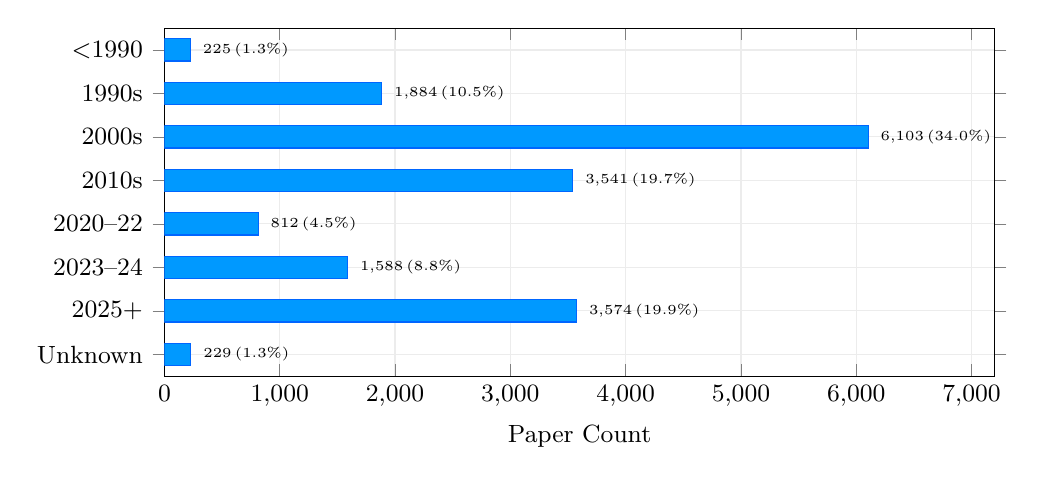
\begin{tikzpicture}
\begin{axis}[
    xbar,
    width=\columnwidth,
    height=6cm,
    xlabel={Paper Count},
    xlabel style={font=\small},
    xmin=0, xmax=7200,
    ytick=data,
    yticklabels={
        {$<$1990},
        {1990s},
        {2000s},
        {2010s},
        {2020--22},
        {2023--24},
        {2025+},
        {Unknown}
    },
    yticklabel style={font=\small},
    y dir=reverse,
    bar width=8pt,
    nodes near coords,
    nodes near coords style={font=\tiny, anchor=west},
    every node near coord/.append style={xshift=1pt},
    enlarge y limits={abs=0.5},
    grid=major,
    grid style={gray!15},
    xticklabel style={font=\small},
    point meta=explicit symbolic,
]
\addplot[fill=blue!40!cyan, draw=blue!60!cyan] coordinates {
    (225,0)  [225\,(1.3\%)]
    (1884,1) [1{,}884\,(10.5\%)]
    (6103,2) [6{,}103\,(34.0\%)]
    (3541,3) [3{,}541\,(19.7\%)]
    (812,4)  [812\,(4.5\%)]
    (1588,5) [1{,}588\,(8.8\%)]
    (3574,6) [3{,}574\,(19.9\%)]
    (229,7)  [229\,(1.3\%)]
};
\end{axis}
\end{tikzpicture}
\caption{\textbf{Era breakdown} of the 17,956 high-relevance papers in the
Sutra Corpus. The 2000s peak (34\%) reflects classical MAS's golden age.
The 2010s dip precedes the LLM-agent explosion (2025+: 19.9\%).
Data source: Sutra Pipeline database.}
\label{fig:era-breakdown}
\end{figure}


\begin{figure}[t]
\centering
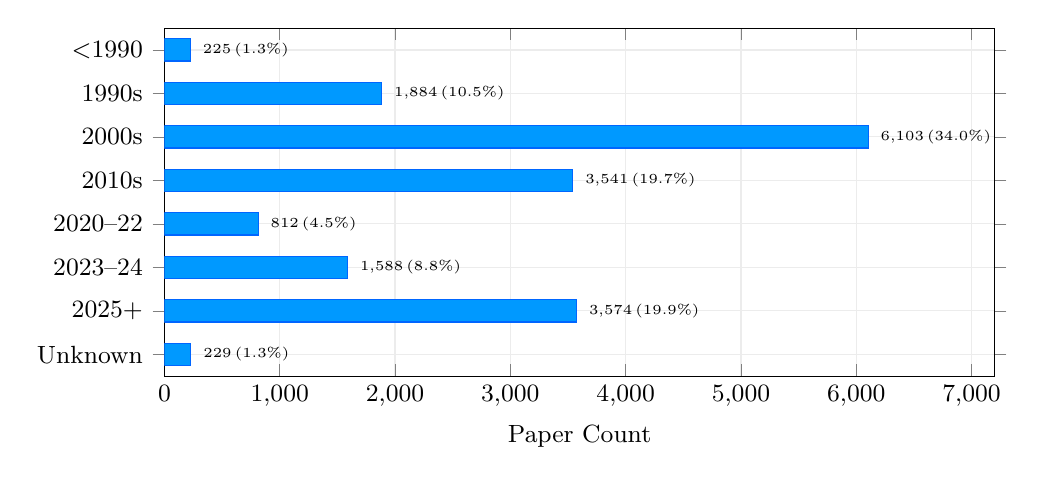
\begin{tikzpicture}
\begin{axis}[
    xbar,
    width=\columnwidth,
    height=6cm,
    xlabel={Paper Count},
    xlabel style={font=\small},
    xmin=0, xmax=7200,
    ytick=data,
    yticklabels={
        {$<$1990},
        {1990s},
        {2000s},
        {2010s},
        {2020--22},
        {2023--24},
        {2025+},
        {Unknown}
    },
    yticklabel style={font=\small},
    y dir=reverse,
    bar width=8pt,
    nodes near coords,
    nodes near coords style={font=\tiny, anchor=west},
    every node near coord/.append style={xshift=1pt},
    enlarge y limits={abs=0.5},
    grid=major,
    grid style={gray!15},
    xticklabel style={font=\small},
    point meta=explicit symbolic,
]
\addplot[fill=blue!40!cyan, draw=blue!60!cyan] coordinates {
    (225,0)  [225\,(1.3\%)]
    (1884,1) [1{,}884\,(10.5\%)]
    (6103,2) [6{,}103\,(34.0\%)]
    (3541,3) [3{,}541\,(19.7\%)]
    (812,4)  [812\,(4.5\%)]
    (1588,5) [1{,}588\,(8.8\%)]
    (3574,6) [3{,}574\,(19.9\%)]
    (229,7)  [229\,(1.3\%)]
};
\end{axis}
\end{tikzpicture}
\caption{\textbf{Era breakdown} of the 17,956 high-relevance papers in the
Sutra Corpus. The 2000s peak (34\%) reflects classical MAS's golden age.
The 2010s dip precedes the LLM-agent explosion (2025+: 19.9\%).
Data source: Sutra Pipeline database.}
\label{fig:era-breakdown}
\end{figure}


\begin{figure}[t]
\centering
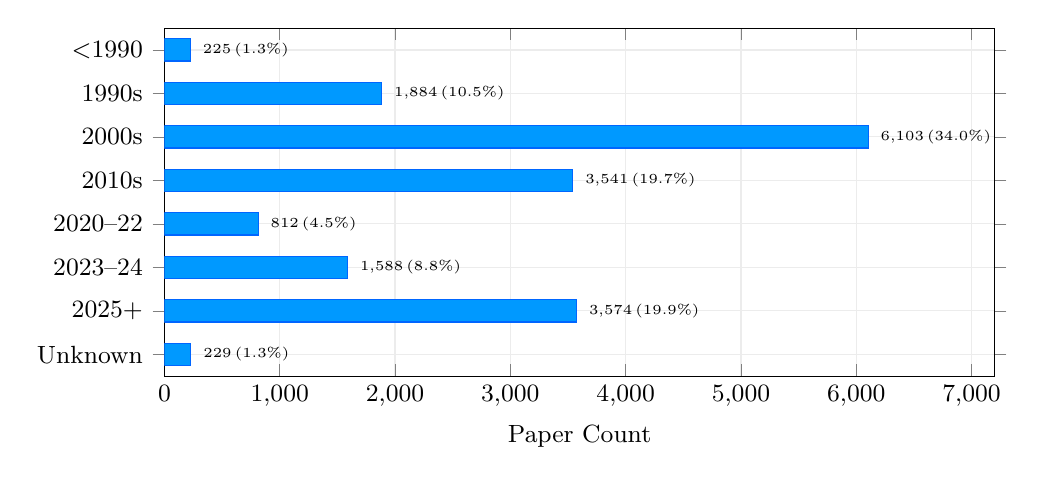
\begin{tikzpicture}
\begin{axis}[
    xbar,
    width=\columnwidth,
    height=6cm,
    xlabel={Paper Count},
    xlabel style={font=\small},
    xmin=0, xmax=7200,
    ytick=data,
    yticklabels={
        {$<$1990},
        {1990s},
        {2000s},
        {2010s},
        {2020--22},
        {2023--24},
        {2025+},
        {Unknown}
    },
    yticklabel style={font=\small},
    y dir=reverse,
    bar width=8pt,
    nodes near coords,
    nodes near coords style={font=\tiny, anchor=west},
    every node near coord/.append style={xshift=1pt},
    enlarge y limits={abs=0.5},
    grid=major,
    grid style={gray!15},
    xticklabel style={font=\small},
    point meta=explicit symbolic,
]
\addplot[fill=blue!40!cyan, draw=blue!60!cyan] coordinates {
    (225,0)  [225\,(1.3\%)]
    (1884,1) [1{,}884\,(10.5\%)]
    (6103,2) [6{,}103\,(34.0\%)]
    (3541,3) [3{,}541\,(19.7\%)]
    (812,4)  [812\,(4.5\%)]
    (1588,5) [1{,}588\,(8.8\%)]
    (3574,6) [3{,}574\,(19.9\%)]
    (229,7)  [229\,(1.3\%)]
};
\end{axis}
\end{tikzpicture}
\caption{\textbf{Era breakdown} of the 17,956 high-relevance papers in the
Sutra Corpus. The 2000s peak (34\%) reflects classical MAS's golden age.
The 2010s dip precedes the LLM-agent explosion (2025+: 19.9\%).
Data source: Sutra Pipeline database.}
\label{fig:era-breakdown}
\end{figure}

% Figure: Citation Distribution across the Sutra Corpus
% Data source: Sutra Pipeline database, 17,956 high-relevance papers
% Usage: % Figure: Citation Distribution across the Sutra Corpus
% Data source: Sutra Pipeline database, 17,956 high-relevance papers
% Usage: % Figure: Citation Distribution across the Sutra Corpus
% Data source: Sutra Pipeline database, 17,956 high-relevance papers
% Usage: \input{figures/citation-distribution.tex}

\begin{figure}[t]
\centering
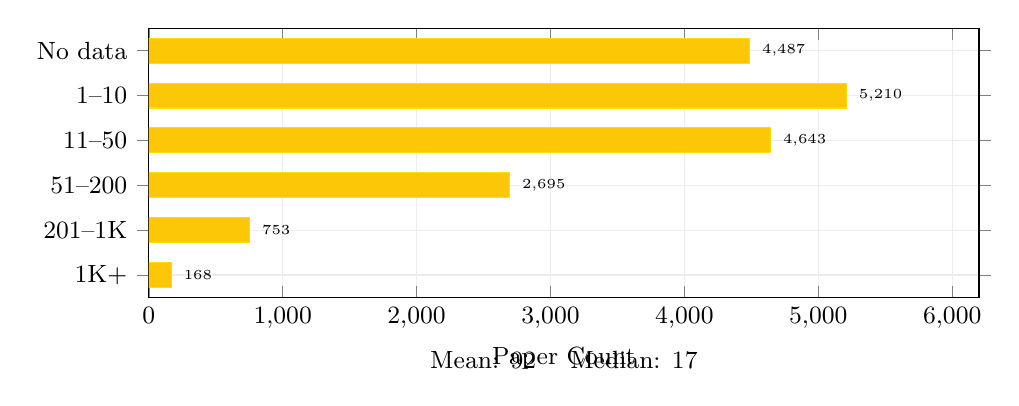
\begin{tikzpicture}
\begin{axis}[
    xbar,
    width=\columnwidth,
    height=5cm,
    xlabel={Paper Count},
    xlabel style={font=\small},
    xmin=0, xmax=6200,
    ytick=data,
    yticklabels={
        {No data},
        {1--10},
        {11--50},
        {51--200},
        {201--1K},
        {1K+}
    },
    yticklabel style={font=\small},
    y dir=reverse,
    bar width=9pt,
    nodes near coords,
    nodes near coords style={font=\tiny, anchor=west},
    every node near coord/.append style={xshift=1pt},
    enlarge y limits={abs=0.5},
    grid=major,
    grid style={gray!15},
    xticklabel style={font=\small},
    point meta=explicit symbolic,
    title={\small Mean: 92 \quad Median: 17},
    title style={at={(0.5,0)}, anchor=north, yshift=-22pt},
]
\addplot[fill=yellow!60!orange, draw=yellow!80!orange] coordinates {
    (4487,0) [4{,}487]
    (5210,1) [5{,}210]
    (4643,2) [4{,}643]
    (2695,3) [2{,}695]
    (753,4)  [753]
    (168,5)  [168]
};
\end{axis}
\end{tikzpicture}
\caption{\textbf{Citation distribution} across the Sutra Corpus.
The power-law shape (mean 92, median 17) reflects a small number of
foundational papers accumulating thousands of citations while most
have modest impact.}
\label{fig:cite-distribution}
\end{figure}


\begin{figure}[t]
\centering
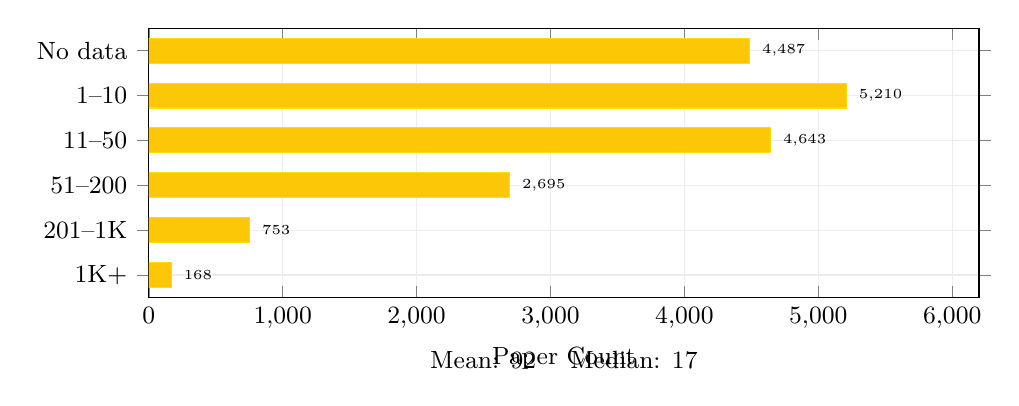
\begin{tikzpicture}
\begin{axis}[
    xbar,
    width=\columnwidth,
    height=5cm,
    xlabel={Paper Count},
    xlabel style={font=\small},
    xmin=0, xmax=6200,
    ytick=data,
    yticklabels={
        {No data},
        {1--10},
        {11--50},
        {51--200},
        {201--1K},
        {1K+}
    },
    yticklabel style={font=\small},
    y dir=reverse,
    bar width=9pt,
    nodes near coords,
    nodes near coords style={font=\tiny, anchor=west},
    every node near coord/.append style={xshift=1pt},
    enlarge y limits={abs=0.5},
    grid=major,
    grid style={gray!15},
    xticklabel style={font=\small},
    point meta=explicit symbolic,
    title={\small Mean: 92 \quad Median: 17},
    title style={at={(0.5,0)}, anchor=north, yshift=-22pt},
]
\addplot[fill=yellow!60!orange, draw=yellow!80!orange] coordinates {
    (4487,0) [4{,}487]
    (5210,1) [5{,}210]
    (4643,2) [4{,}643]
    (2695,3) [2{,}695]
    (753,4)  [753]
    (168,5)  [168]
};
\end{axis}
\end{tikzpicture}
\caption{\textbf{Citation distribution} across the Sutra Corpus.
The power-law shape (mean 92, median 17) reflects a small number of
foundational papers accumulating thousands of citations while most
have modest impact.}
\label{fig:cite-distribution}
\end{figure}


\begin{figure}[t]
\centering
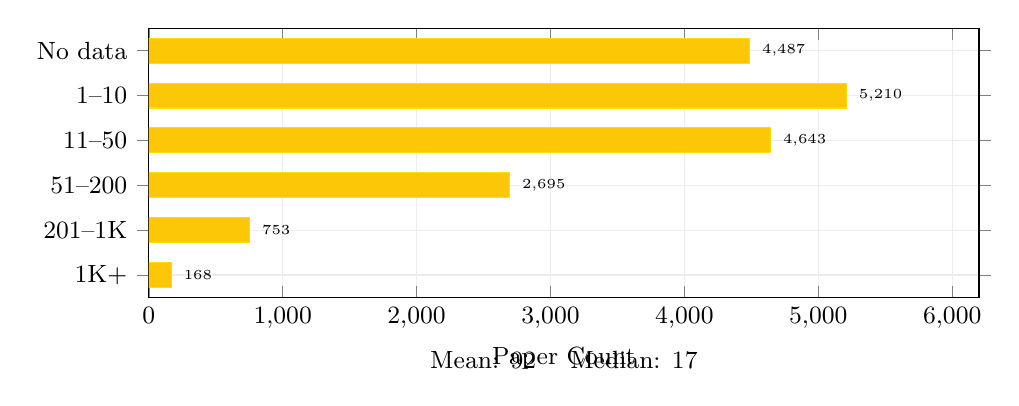
\begin{tikzpicture}
\begin{axis}[
    xbar,
    width=\columnwidth,
    height=5cm,
    xlabel={Paper Count},
    xlabel style={font=\small},
    xmin=0, xmax=6200,
    ytick=data,
    yticklabels={
        {No data},
        {1--10},
        {11--50},
        {51--200},
        {201--1K},
        {1K+}
    },
    yticklabel style={font=\small},
    y dir=reverse,
    bar width=9pt,
    nodes near coords,
    nodes near coords style={font=\tiny, anchor=west},
    every node near coord/.append style={xshift=1pt},
    enlarge y limits={abs=0.5},
    grid=major,
    grid style={gray!15},
    xticklabel style={font=\small},
    point meta=explicit symbolic,
    title={\small Mean: 92 \quad Median: 17},
    title style={at={(0.5,0)}, anchor=north, yshift=-22pt},
]
\addplot[fill=yellow!60!orange, draw=yellow!80!orange] coordinates {
    (4487,0) [4{,}487]
    (5210,1) [5{,}210]
    (4643,2) [4{,}643]
    (2695,3) [2{,}695]
    (753,4)  [753]
    (168,5)  [168]
};
\end{axis}
\end{tikzpicture}
\caption{\textbf{Citation distribution} across the Sutra Corpus.
The power-law shape (mean 92, median 17) reflects a small number of
foundational papers accumulating thousands of citations while most
have modest impact.}
\label{fig:cite-distribution}
\end{figure}


\subsection{Lost Canaries Found}
\label{sec:res-canaries}

% --- PLAN ---
% 18 root primitives -> 6 candidates -> 3-way classification:
%   4 genuinely lost: Joint Persistent Goals, Discourse Coherence,
%     Formal Responsibility, Social Knowledge Semantics
%   1 known-but-ignored: [to be confirmed by author]
%   8 renamed without citation: DAI, Contract Net, DPS Frameworks,
%     Negotiation Protocols, etc.
%
% The initial classification table (13 candidates):
%   Paper | Year | Total Cites | Modernity | Classification
%   [Full 13-row table from contributions.md C3]
%
% The aggregate signal: top 10 "missing classical concepts" from
% 17,971 papers (bottom-up LLM assessment):
%   Organizational Models: 5,556
%   BDI: 4,166
%   FIPA Protocols: 3,882
%   Contract Net: 3,310
%   Blackboard: 2,051
%   MOISE/AGR: 2,037
%   SharedPlans: 1,855
%   Joint Intentions: 1,570
%   Auction/Mechanism Design: 1,288
%   Consensus Protocols: 902
%
% TRIANGULATION: bottom-up (LLM-flagged) correlates with top-down
%   (citation-based modernity scores). This convergence from two
%   independent methods is strong evidence.
%
% FIGURE: The Citation Cliff -- the SIGNATURE figure of the paper
%   (Figure 3)
%   X-axis: time (1980-2026), Y-axis: citations/year per concept
%   Each line: a classical concept (Contract Net, Blackboard, BDI,
%     SharedPlans, FA/C, Joint Intentions, etc.)
%   Color: whether the concept was reinvented (renamed) or genuinely
%     lost
%   Potential overlay: Cemri failure rates mapped to the year each
%     concept was forgotten
%
% Source: contributions.md C3, pipeline data JSONs

The Lost Canary Algorithm (Section~\ref{sec:meth-canary}) applied to the 22 classical
seeds identified 18 root primitives, from which 6 exceeded both the citation threshold
($>$500) and the modernity threshold ($<$0.05). Concept tracing with the three
anti-false-positive checks produced a three-way classification:

\begin{center}
\footnotesize
\begin{tabular}{@{} r p{2.5cm} r r r l @{}}
\toprule
\textbf{\#} & \textbf{Paper} & \textbf{Yr} & \textbf{Cites} & \textbf{Mod.} & \textbf{Class.} \\
\midrule
1 & Distributed AI & 1987 & 840 & .000 & Renamed \\
2 & Davis \& Smith, Negot. & 1983 & 1231 & .010 & Renamed \\
3 & Durfee \& Lesser, DPS & 1981 & 648 & .014 & Lost Canary \\
4 & Jennings, Joint Int. & 1995 & 551 & .015 & Lost Canary \\
5 & Cohen \& Levesque & 1990 & 1847 & .028 & Lost Canary \\
6 & Bond \& Gasser, DAI & 1988 & 993 & .028 & Lost Canary \\
\bottomrule
\end{tabular}
\end{center}

\noindent
The full initial classification of all 13 candidates (including 7 below the citation
threshold) appears in Appendix~\ref{app:corpus}. The three-way classification:

\begin{itemize}[nosep]
  \item \textbf{Genuinely Lost (4)}: Joint Persistent Goals, Discourse Coherence,
    Formal Responsibility, Social Knowledge Semantics---concepts with no modern
    equivalent and no evidence of concept diffusion through intermediaries.
  \item \textbf{Known but Ignored (1)}: Identified by survey citation check---modern
    surveys cite the concept, but implementation papers do not adopt it.
  \item \textbf{Renamed without Citation (8)}: DAI, Contract Net, DPS Frameworks,
    Negotiation Protocols, and others---concepts that persist under different names
    (``task routing'' for Contract Net, ``shared state'' for blackboard) but without
    citing the originals.
\end{itemize}

\paragraph{The aggregate signal.}
Agent~3b's \texttt{classical\_concepts\_missing} field, aggregated across all 17,955
analyzed papers, produces a bottom-up ``Missing Classical Concepts'' ranking
(Figure~\ref{fig:lost-canary-signal}):

\begin{center}
\begin{tabular}{@{} l r @{}}
\toprule
\textbf{Missing Concept} & \textbf{Papers Flagging It} \\
\midrule
Organizational Models & 8,018 \\
BDI & 5,582 \\
FIPA Protocols & 5,351 \\
Contract Net & 4,686 \\
MOISE/AGR & 2,969 \\
SharedPlans & 2,850 \\
Joint Intentions & 2,547 \\
Blackboard & 2,277 \\
Auction/Mechanism Design & 2,052 \\
Normative MAS & 1,342 \\
\bottomrule
\end{tabular}
\end{center}

% Figure: Coordination Patterns detected by Agent 3b
% Data source: Sutra Pipeline database, 17,955 analyzed papers
% Usage: % Figure: Coordination Patterns detected by Agent 3b
% Data source: Sutra Pipeline database, 17,955 analyzed papers
% Usage: % Figure: Coordination Patterns detected by Agent 3b
% Data source: Sutra Pipeline database, 17,955 analyzed papers
% Usage: \input{figures/coordination-patterns.tex}

\begin{figure}[t]
\centering
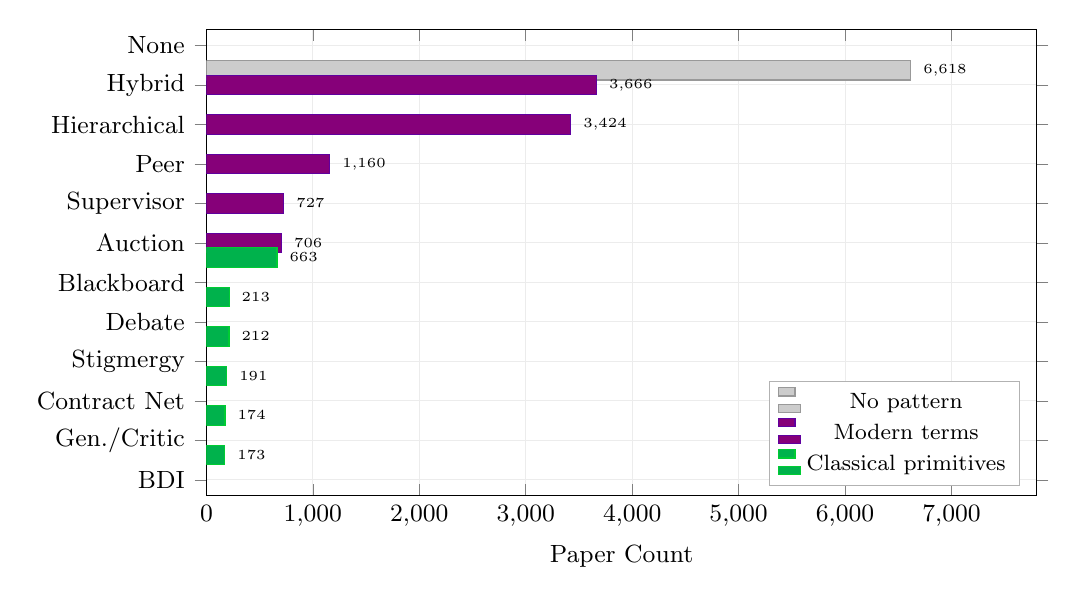
\begin{tikzpicture}
\begin{axis}[
    xbar,
    width=\columnwidth,
    height=7.5cm,
    xlabel={Paper Count},
    xlabel style={font=\small},
    xmin=0, xmax=7800,
    ytick={0,1,2,3,4,5,6,7,8,9,10,11},
    yticklabels={
        {None},
        {Hybrid},
        {Hierarchical},
        {Peer},
        {Supervisor},
        {Auction},
        {Blackboard},
        {Debate},
        {Stigmergy},
        {Contract Net},
        {Gen./Critic},
        {BDI}
    },
    yticklabel style={font=\small},
    y dir=reverse,
    bar width=7pt,
    nodes near coords,
    nodes near coords style={font=\tiny, anchor=west},
    every node near coord/.append style={xshift=1pt},
    enlarge y limits={abs=0.4},
    grid=major,
    grid style={gray!15},
    xticklabel style={font=\small},
    point meta=explicit symbolic,
    legend style={
        at={(0.98,0.02)},
        anchor=south east,
        font=\footnotesize,
        draw=black!30,
    },
]

% None (gray)
\addplot[fill=black!20, draw=black!40] coordinates {
    (6618,0) [6{,}618]
};
\addlegendentry{No pattern}

% Modern coordination terms (purple)
\addplot[fill=blue!30!purple, draw=blue!50!purple] coordinates {
    (3666,1) [3{,}666]
    (3424,2) [3{,}424]
    (1160,3) [1{,}160]
    (727,4)  [727]
    (706,5)  [706]
};
\addlegendentry{Modern terms}

% Classical primitives (green)
\addplot[fill=green!40!teal, draw=green!60!teal] coordinates {
    (663,6)  [663]
    (213,7)  [213]
    (212,8)  [212]
    (191,9)  [191]
    (174,10) [174]
    (173,11) [173]
};
\addlegendentry{Classical primitives}

\end{axis}
\end{tikzpicture}
\caption{\textbf{Coordination patterns} detected by Agent~3b across 17,955
analyzed papers. 37\% have no identifiable coordination pattern. Among
patterned papers, hybrid and hierarchical dominate. Classical primitives
(blackboard, stigmergy, contract net, BDI) appear in only 1,413
papers---the terminology has shifted even when the mechanism persists.}
\label{fig:coord-patterns}
\end{figure}


\begin{figure}[t]
\centering
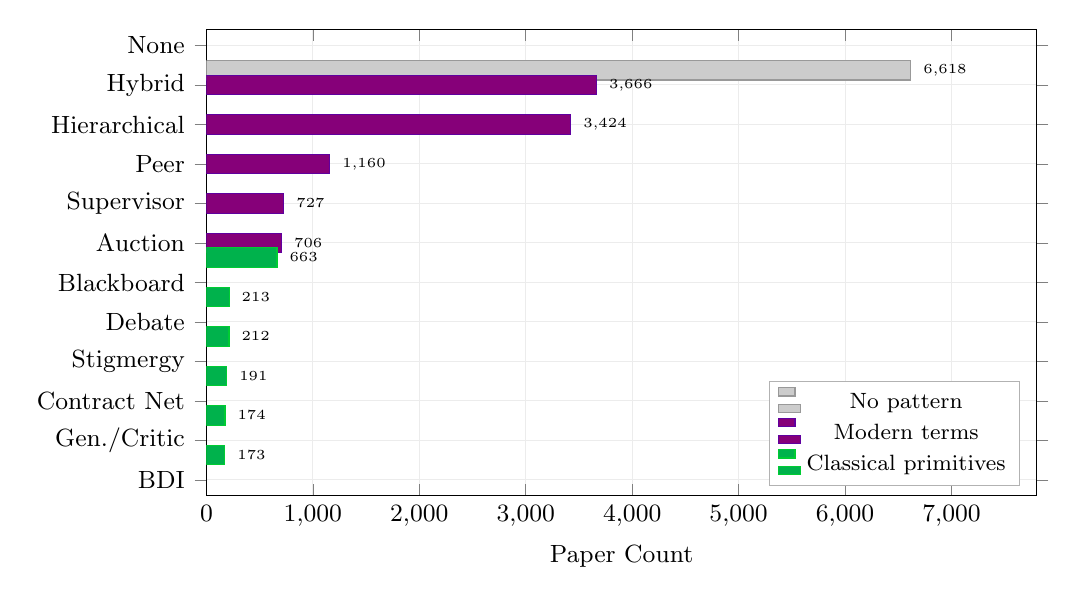
\begin{tikzpicture}
\begin{axis}[
    xbar,
    width=\columnwidth,
    height=7.5cm,
    xlabel={Paper Count},
    xlabel style={font=\small},
    xmin=0, xmax=7800,
    ytick={0,1,2,3,4,5,6,7,8,9,10,11},
    yticklabels={
        {None},
        {Hybrid},
        {Hierarchical},
        {Peer},
        {Supervisor},
        {Auction},
        {Blackboard},
        {Debate},
        {Stigmergy},
        {Contract Net},
        {Gen./Critic},
        {BDI}
    },
    yticklabel style={font=\small},
    y dir=reverse,
    bar width=7pt,
    nodes near coords,
    nodes near coords style={font=\tiny, anchor=west},
    every node near coord/.append style={xshift=1pt},
    enlarge y limits={abs=0.4},
    grid=major,
    grid style={gray!15},
    xticklabel style={font=\small},
    point meta=explicit symbolic,
    legend style={
        at={(0.98,0.02)},
        anchor=south east,
        font=\footnotesize,
        draw=black!30,
    },
]

% None (gray)
\addplot[fill=black!20, draw=black!40] coordinates {
    (6618,0) [6{,}618]
};
\addlegendentry{No pattern}

% Modern coordination terms (purple)
\addplot[fill=blue!30!purple, draw=blue!50!purple] coordinates {
    (3666,1) [3{,}666]
    (3424,2) [3{,}424]
    (1160,3) [1{,}160]
    (727,4)  [727]
    (706,5)  [706]
};
\addlegendentry{Modern terms}

% Classical primitives (green)
\addplot[fill=green!40!teal, draw=green!60!teal] coordinates {
    (663,6)  [663]
    (213,7)  [213]
    (212,8)  [212]
    (191,9)  [191]
    (174,10) [174]
    (173,11) [173]
};
\addlegendentry{Classical primitives}

\end{axis}
\end{tikzpicture}
\caption{\textbf{Coordination patterns} detected by Agent~3b across 17,955
analyzed papers. 37\% have no identifiable coordination pattern. Among
patterned papers, hybrid and hierarchical dominate. Classical primitives
(blackboard, stigmergy, contract net, BDI) appear in only 1,413
papers---the terminology has shifted even when the mechanism persists.}
\label{fig:coord-patterns}
\end{figure}


\begin{figure}[t]
\centering
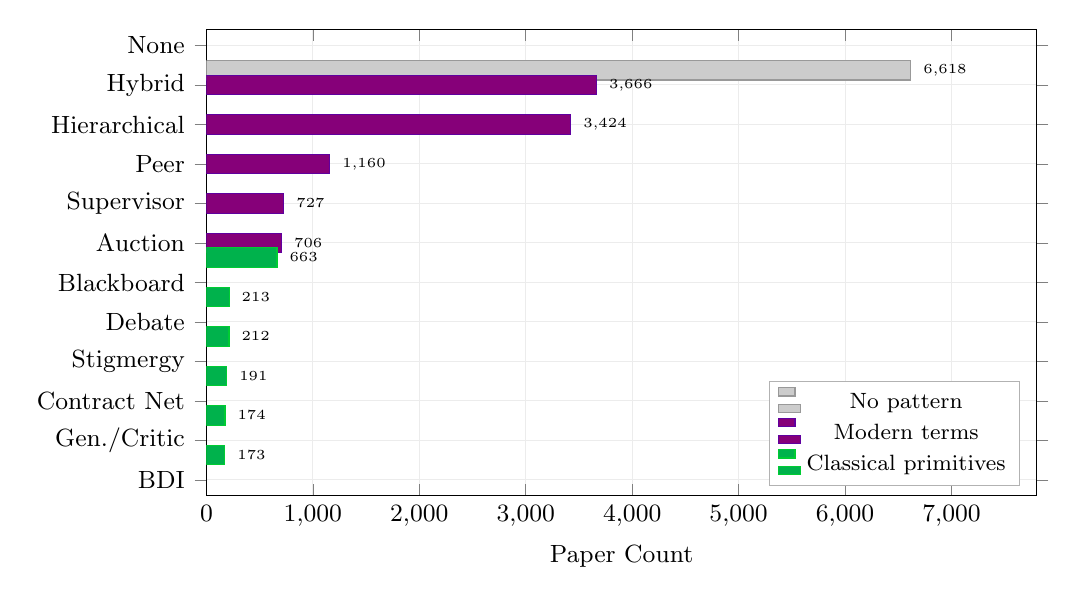
\begin{tikzpicture}
\begin{axis}[
    xbar,
    width=\columnwidth,
    height=7.5cm,
    xlabel={Paper Count},
    xlabel style={font=\small},
    xmin=0, xmax=7800,
    ytick={0,1,2,3,4,5,6,7,8,9,10,11},
    yticklabels={
        {None},
        {Hybrid},
        {Hierarchical},
        {Peer},
        {Supervisor},
        {Auction},
        {Blackboard},
        {Debate},
        {Stigmergy},
        {Contract Net},
        {Gen./Critic},
        {BDI}
    },
    yticklabel style={font=\small},
    y dir=reverse,
    bar width=7pt,
    nodes near coords,
    nodes near coords style={font=\tiny, anchor=west},
    every node near coord/.append style={xshift=1pt},
    enlarge y limits={abs=0.4},
    grid=major,
    grid style={gray!15},
    xticklabel style={font=\small},
    point meta=explicit symbolic,
    legend style={
        at={(0.98,0.02)},
        anchor=south east,
        font=\footnotesize,
        draw=black!30,
    },
]

% None (gray)
\addplot[fill=black!20, draw=black!40] coordinates {
    (6618,0) [6{,}618]
};
\addlegendentry{No pattern}

% Modern coordination terms (purple)
\addplot[fill=blue!30!purple, draw=blue!50!purple] coordinates {
    (3666,1) [3{,}666]
    (3424,2) [3{,}424]
    (1160,3) [1{,}160]
    (727,4)  [727]
    (706,5)  [706]
};
\addlegendentry{Modern terms}

% Classical primitives (green)
\addplot[fill=green!40!teal, draw=green!60!teal] coordinates {
    (663,6)  [663]
    (213,7)  [213]
    (212,8)  [212]
    (191,9)  [191]
    (174,10) [174]
    (173,11) [173]
};
\addlegendentry{Classical primitives}

\end{axis}
\end{tikzpicture}
\caption{\textbf{Coordination patterns} detected by Agent~3b across 17,955
analyzed papers. 37\% have no identifiable coordination pattern. Among
patterned papers, hybrid and hierarchical dominate. Classical primitives
(blackboard, stigmergy, contract net, BDI) appear in only 1,413
papers---the terminology has shifted even when the mechanism persists.}
\label{fig:coord-patterns}
\end{figure}

% Figure: Lost Canary Signal — Missing Classical Concepts
% Data source: Sutra Pipeline database, Agent 3b's classical_concepts_missing field
% Usage: % Figure: Lost Canary Signal — Missing Classical Concepts
% Data source: Sutra Pipeline database, Agent 3b's classical_concepts_missing field
% Usage: % Figure: Lost Canary Signal — Missing Classical Concepts
% Data source: Sutra Pipeline database, Agent 3b's classical_concepts_missing field
% Usage: \input{figures/lost-canary-signal.tex}

\begin{figure}[t]
\centering
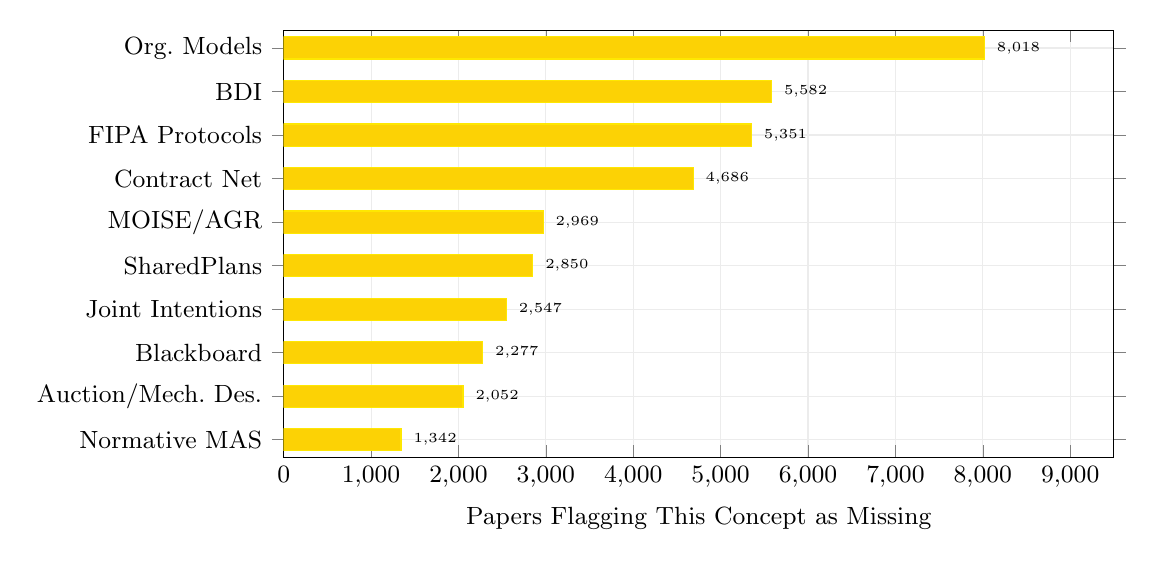
\begin{tikzpicture}
\begin{axis}[
    xbar,
    width=\columnwidth,
    height=7cm,
    xlabel={Papers Flagging This Concept as Missing},
    xlabel style={font=\small},
    xmin=0, xmax=9500,
    ytick=data,
    yticklabels={
        {Org.\ Models},
        {BDI},
        {FIPA Protocols},
        {Contract Net},
        {MOISE/AGR},
        {SharedPlans},
        {Joint Intentions},
        {Blackboard},
        {Auction/Mech.\ Des.},
        {Normative MAS}
    },
    yticklabel style={font=\small},
    y dir=reverse,
    bar width=8pt,
    nodes near coords,
    nodes near coords style={font=\tiny, anchor=west},
    every node near coord/.append style={xshift=1pt},
    enlarge y limits={abs=0.4},
    grid=major,
    grid style={gray!15},
    xticklabel style={font=\small},
    point meta=explicit symbolic,
]
\addplot[fill=yellow!70!orange, draw=yellow!90!orange] coordinates {
    (8018,0) [8{,}018]
    (5582,1) [5{,}582]
    (5351,2) [5{,}351]
    (4686,3) [4{,}686]
    (2969,4) [2{,}969]
    (2850,5) [2{,}850]
    (2547,6) [2{,}547]
    (2277,7) [2{,}277]
    (2052,8) [2{,}052]
    (1342,9) [1{,}342]
};
\end{axis}
\end{tikzpicture}
\caption{\textbf{Lost Canary Signal}: classical concepts flagged as missing
by Agent~3b's \texttt{classical\_concepts\_missing} field, aggregated across
17,955 analyzed papers. Organizational Models (8,018) and BDI (5,582) are
most frequently absent from modern work---well-solved concepts in the
classical literature that LLM-agent implementations ignore.}
\label{fig:lost-canary-signal}
\end{figure}


\begin{figure}[t]
\centering
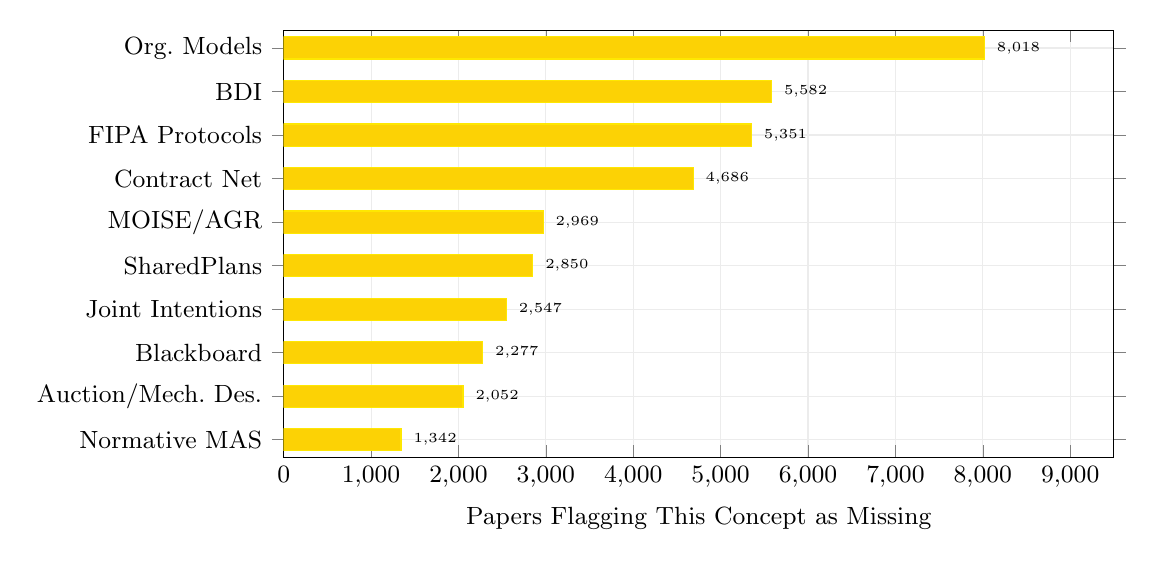
\begin{tikzpicture}
\begin{axis}[
    xbar,
    width=\columnwidth,
    height=7cm,
    xlabel={Papers Flagging This Concept as Missing},
    xlabel style={font=\small},
    xmin=0, xmax=9500,
    ytick=data,
    yticklabels={
        {Org.\ Models},
        {BDI},
        {FIPA Protocols},
        {Contract Net},
        {MOISE/AGR},
        {SharedPlans},
        {Joint Intentions},
        {Blackboard},
        {Auction/Mech.\ Des.},
        {Normative MAS}
    },
    yticklabel style={font=\small},
    y dir=reverse,
    bar width=8pt,
    nodes near coords,
    nodes near coords style={font=\tiny, anchor=west},
    every node near coord/.append style={xshift=1pt},
    enlarge y limits={abs=0.4},
    grid=major,
    grid style={gray!15},
    xticklabel style={font=\small},
    point meta=explicit symbolic,
]
\addplot[fill=yellow!70!orange, draw=yellow!90!orange] coordinates {
    (8018,0) [8{,}018]
    (5582,1) [5{,}582]
    (5351,2) [5{,}351]
    (4686,3) [4{,}686]
    (2969,4) [2{,}969]
    (2850,5) [2{,}850]
    (2547,6) [2{,}547]
    (2277,7) [2{,}277]
    (2052,8) [2{,}052]
    (1342,9) [1{,}342]
};
\end{axis}
\end{tikzpicture}
\caption{\textbf{Lost Canary Signal}: classical concepts flagged as missing
by Agent~3b's \texttt{classical\_concepts\_missing} field, aggregated across
17,955 analyzed papers. Organizational Models (8,018) and BDI (5,582) are
most frequently absent from modern work---well-solved concepts in the
classical literature that LLM-agent implementations ignore.}
\label{fig:lost-canary-signal}
\end{figure}


\begin{figure}[t]
\centering
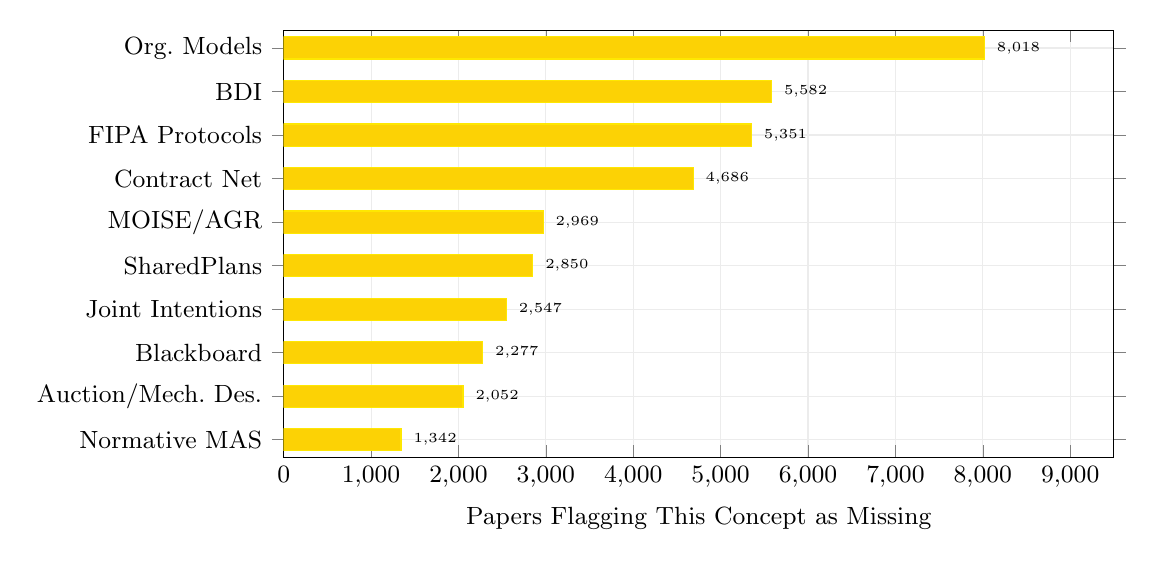
\begin{tikzpicture}
\begin{axis}[
    xbar,
    width=\columnwidth,
    height=7cm,
    xlabel={Papers Flagging This Concept as Missing},
    xlabel style={font=\small},
    xmin=0, xmax=9500,
    ytick=data,
    yticklabels={
        {Org.\ Models},
        {BDI},
        {FIPA Protocols},
        {Contract Net},
        {MOISE/AGR},
        {SharedPlans},
        {Joint Intentions},
        {Blackboard},
        {Auction/Mech.\ Des.},
        {Normative MAS}
    },
    yticklabel style={font=\small},
    y dir=reverse,
    bar width=8pt,
    nodes near coords,
    nodes near coords style={font=\tiny, anchor=west},
    every node near coord/.append style={xshift=1pt},
    enlarge y limits={abs=0.4},
    grid=major,
    grid style={gray!15},
    xticklabel style={font=\small},
    point meta=explicit symbolic,
]
\addplot[fill=yellow!70!orange, draw=yellow!90!orange] coordinates {
    (8018,0) [8{,}018]
    (5582,1) [5{,}582]
    (5351,2) [5{,}351]
    (4686,3) [4{,}686]
    (2969,4) [2{,}969]
    (2850,5) [2{,}850]
    (2547,6) [2{,}547]
    (2277,7) [2{,}277]
    (2052,8) [2{,}052]
    (1342,9) [1{,}342]
};
\end{axis}
\end{tikzpicture}
\caption{\textbf{Lost Canary Signal}: classical concepts flagged as missing
by Agent~3b's \texttt{classical\_concepts\_missing} field, aggregated across
17,955 analyzed papers. Organizational Models (8,018) and BDI (5,582) are
most frequently absent from modern work---well-solved concepts in the
classical literature that LLM-agent implementations ignore.}
\label{fig:lost-canary-signal}
\end{figure}


\paragraph{Triangulation.}
The bottom-up signal (LLM-flagged missing concepts) and the top-down signal
(citation-based modernity scores) converge: the concepts flagged most frequently as
``missing'' by Agent~3b align with the concepts that have the lowest modernity scores
in the citation graph. This convergence from two independent methods---one based on
citation patterns, the other on LLM assessment of individual papers---provides strong
triangulation evidence that the Lost Canary findings reflect genuine gaps in the
literature rather than artifacts of either method alone.

% FIGURE: The Citation Cliff -- the SIGNATURE figure (Figure 3)
% [To be generated from modernity_scores.json counts_by_year data]

\noindent
Both signals are explorable interactively: the Sutra Portal's Citation Cliff
visualization (Section~\ref{sec:res-artifacts}) plots per-year citation trajectories
for all 18 root primitives, and the Reinvention Radar renders the concept-overlap
graph as a filterable bipartite network distinguishing reinvention (uncited) from
acknowledged (cited) connections.

\subsection{The Rosetta Stone}
\label{sec:res-rosetta}

% --- PLAN ---
% The consolidated mapping table (14+ entries with fidelity ratings):
%   Classical Concept | Modern Equivalent | Fidelity | What's Lost
%   Joint Persistent Goals | None | N/A | No shared goal tracking
%   Discourse Coherence | None | N/A | Flat message history
%   Formal Responsibility | None | N/A | No responsibility tracking
%   Social Knowledge | System prompts + roles | Low | No social
%     obligations or commitment protocols
%   Commitment Theory | Agent "memory" | Very Low | Memory stores
%     facts, not commitments; no theory of decommitment
%   Contract Net | Agent routing | Medium | No formal cost models,
%     no self-selection
%   Blackboard | Shared state (LangGraph, Redis) | Medium | Control
%     Shell -- the most valuable part -- is lost
%   FA/C Philosophy | None | N/A | No framework embraces functionally
%     accurate intermediate results
%   Task Environment Modeling | None | N/A | No formal task models
%   Organizational Paradigms | CrewAI roles, AutoGen group chat | Low |
%     Role labels survive but formal org theory absent
%
% Protocol-level mapping (FIPA -> A2A/MCP):
%   TABLE: 9 performatives with modern equivalents and gap analysis
%   Gaps concentrate on negotiation performatives (cfp, propose,
%   accept-proposal, reject-proposal) -- building blocks of
%   Contract Net.
%
% The reinvention edge graph:
%   Bipartite: modern papers (left) -- classical papers (right)
%   Edges: concept overlap. Color: citation exists (green) vs.
%   no citation (red = reinvention).
%
% FIGURE: Reinvention detection bipartite graph (Figure 5)
% FIGURE: The Rosetta Stone table -- full-page (Figure 10)
%
% Source: contributions.md C4, pipeline data

The Rosetta Stone consolidates three data sources into a structured mapping between
classical MAS concepts and their modern LLM-agent equivalents: (1)~a hand-curated table
from the Bridge Builder assessments, (2)~per-paper \texttt{rosetta\_entry} annotations
across 17,971 papers, and (3)~a materialized \texttt{reinvention\_edges} table that
detects concept overlap without citation. Table~\ref{tab:rosetta} presents the
consolidated mapping with fidelity ratings.

\begin{table*}[t]
\centering
\caption{The Rosetta Stone: Classical-to-Modern MAS Mapping with Fidelity Ratings.}
\label{tab:rosetta}
\small
\begin{tabular}{@{} p{4cm} p{3.5cm} l p{5.5cm} @{}}
\toprule
\textbf{Classical Concept} & \textbf{Modern Equivalent} & \textbf{Fidelity} & \textbf{What's Lost in Translation} \\
\midrule
Joint Persistent Goals (Cohen \& Levesque 1990) & None & N/A & No framework tracks shared goals with obligation-to-inform on failure \\
Discourse Coherence (Grosz \& Sidner 1986) & None & N/A & Flat message history; no hierarchy, no discourse purposes \\
Formal Responsibility (1992) & None & N/A & Delegation exists but responsibility tracking does not \\
FA/C Philosophy (Lesser \& Corkill 1983) & None & N/A & No framework embraces functionally accurate intermediate results \\
Task Env.\ Modeling (Decker 1996) & None & N/A & No formal task models; LLMs ``figure it out'' from prompts \\
\midrule
Social Knowledge (Singh 1991) & System prompts + roles & Low & Persona without social obligations or commitment protocols \\
Org.\ Paradigms (Horling \& Lesser 2004) & CrewAI roles, AutoGen group chat & Low & Role labels survive but formal org theory absent \\
Commitment Theory (Cohen \& Levesque 1990) & Agent ``memory'' & Very Low & Memory stores facts, not commitments; no decommitment theory \\
\midrule
Contract Net (Smith 1980) & Agent routing / orchestration & Medium & No formal cost models, no marginal-cost bidding, no self-selection \\
Blackboard (Nii 1986) & Shared state (LangGraph, Redis) & Medium & Control Shell---the most valuable part---is lost \\
\bottomrule
\end{tabular}
\end{table*}

\paragraph{The reinvention graph.}
The \texttt{reinvention\_edges} table detects classical-modern paper pairs with concept
overlap but \emph{missing citations}: for each modern paper (post-2020), we find
classical papers (pre-2010) sharing $\geq$2 concept keywords from Agent~3b's extraction,
then check the \texttt{citation\_edges} table for an actual citation. A
\emph{reinvention} is concept overlap without citation---the modern paper uses the
concept but does not cite the originator. This produces a bipartite graph
with modern papers on one side and classical papers on the other, edges colored by
whether citation exists (green) or is absent (red).%
% TODO: Add reinvention bipartite graph figure

\paragraph{Protocol-level mapping.}
Beyond concept-level mappings, we trace the FIPA interaction protocol library to
its modern equivalents in A2A and MCP (Section~\ref{sec:p-acl}). The gaps concentrate
on \emph{negotiation performatives}---\texttt{cfp}, \texttt{propose},
\texttt{accept-proposal}, \texttt{reject-proposal}---which are the building blocks
of Contract Net. Neither A2A nor MCP provides equivalents, leaving the most important
coordination protocol without infrastructure support.

\subsection{The 16-Segment Taxonomy}
\label{sec:res-taxonomy}

% --- PLAN ---
% The UMAP cluster visualization with reading triples
%
% Per-cluster statistics:
%   - Paper count per cluster
%   - Era split (classical vs. modern)
%   - Landmark / Central / Survey papers identified
%
% Cross-cluster citation patterns:
%   - Which clusters cite each other? Where are the bridges?
%   - Where are the walls? (Clusters with near-zero cross-citation)
%
% FIGURE: The UMAP cluster map -- the "poster figure" (Figure 4)
%
% Source: contributions.md C2, dashboard data

The semi-supervised taxonomy method (Section~\ref{sec:meth-taxonomy}) assigns all
corpus papers to 16 segments, each corresponding to a pillar of MAS research surveyed
in Section~\ref{sec:pillars}. For each segment, we report paper count, era split,
and the reading triple:

\begin{table}[h]
\centering
\caption{The 16-segment taxonomy: paper counts and temporal profile. Classical\%
denotes the fraction of papers published before 2015; Modern\% denotes 2023 onward.}
\label{tab:taxonomy-temporal}
\footnotesize
\begin{tabular}{@{} r p{3.8cm} r r r @{}}
\toprule
\textbf{ID} & \textbf{Segment} & \textbf{Papers} & \textbf{Cl.\%} & \textbf{Mod.\%} \\
\midrule
0 & Shared Medium Coord. & 1,089 & 55 & 39 \\
1 & Contract Net \& Allocation & 942 & 84 & 6 \\
2 & Org.\ Design \& Teams & 2,132 & 54 & 37 \\
3 & Planning, DPS \& Teamwork & 1,792 & 71 & 13 \\
4 & ACL \& Protocols & 279 & 87 & 7 \\
5 & Argumentation \& Debate & 385 & 45 & 39 \\
6 & Negotiation \& Game Theory & 1,166 & 69 & 11 \\
7 & BDI \& Cognitive Arch. & 1,951 & 59 & 32 \\
8 & Human-Agent \& HITL & 332 & 25 & 61 \\
9 & Trust, Reputation \& Norms & 657 & 77 & 11 \\
10 & Engineering \& Frameworks & 2,385 & 72 & 23 \\
11 & Robotics \& Embodied & 920 & 63 & 10 \\
12 & Eval.\ \& Failure Analysis & 912 & 35 & 57 \\
13 & Memory \& Context & 106 & 7 & 89 \\
14 & Learning \& Adaptation & 2,326 & 30 & 48 \\
15 & Artificial Societies & 365 & 66 & 25 \\
\midrule
\multicolumn{2}{@{}l}{\textbf{Total}} & \textbf{17,969} & & \\
\bottomrule
\end{tabular}
\end{table}

\begin{figure}[t]
\centering
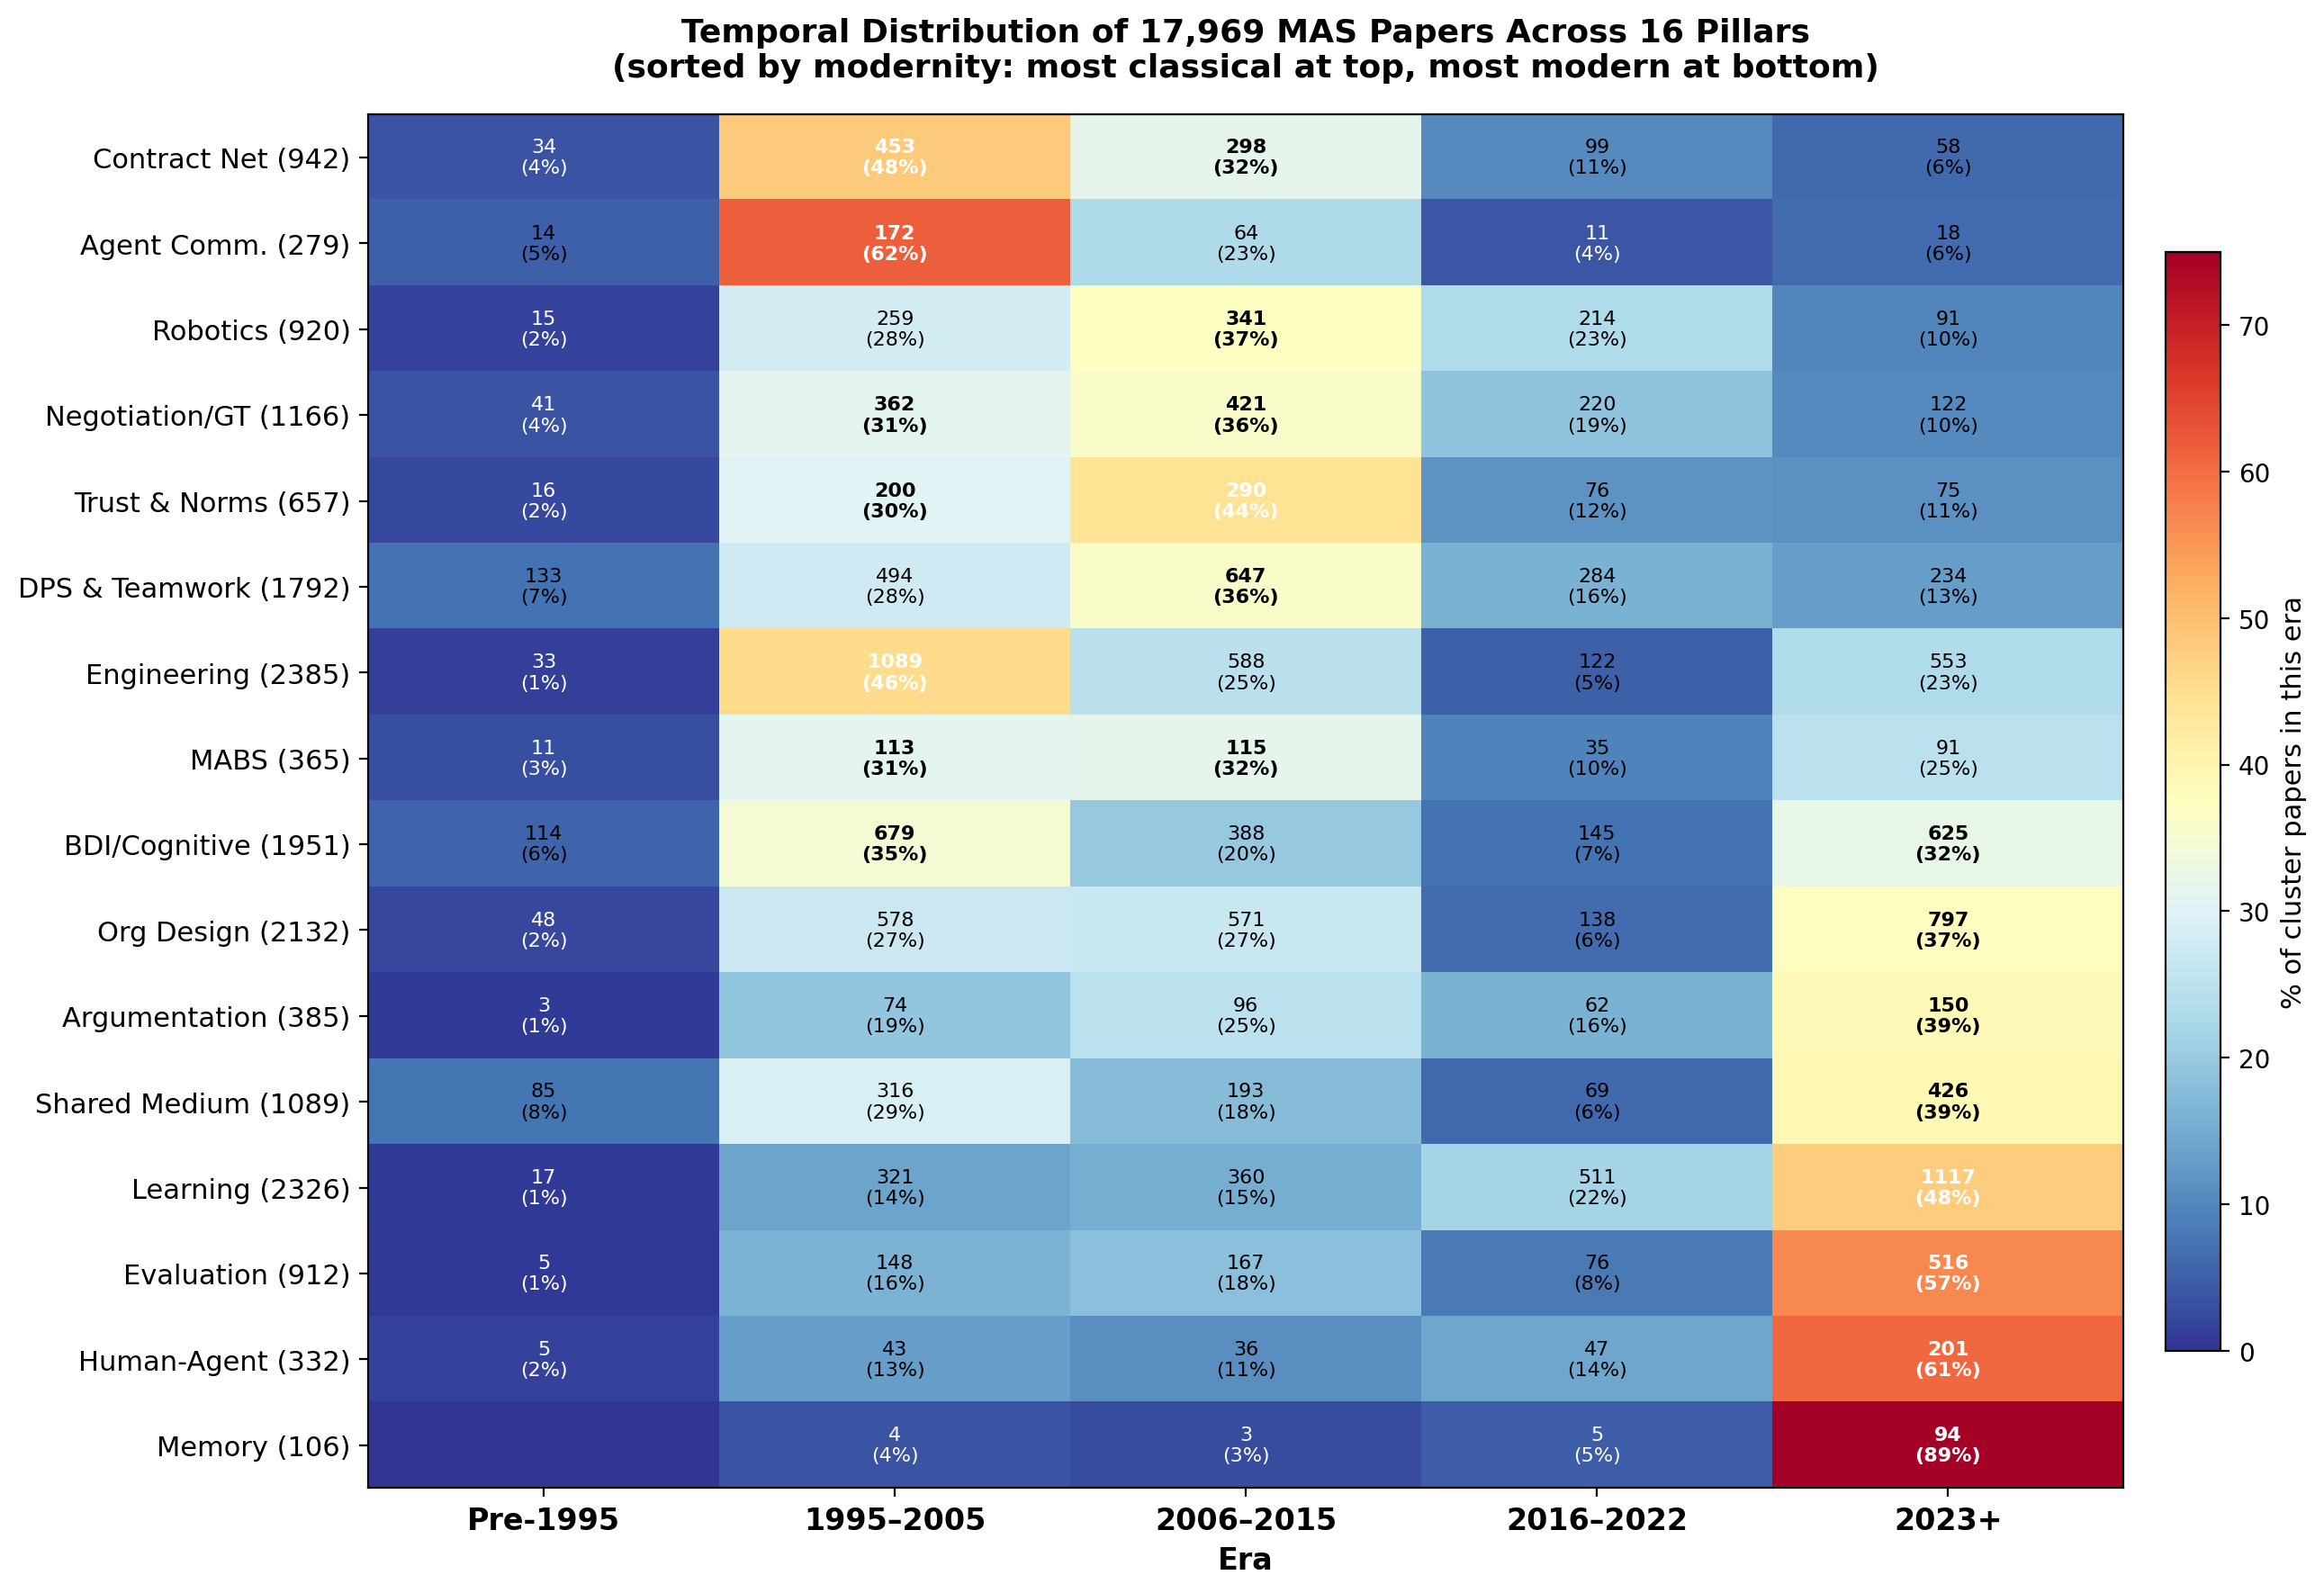
\includegraphics[width=\linewidth]{figures/temporal_heatmap.png}
\caption{Temporal heatmap of MAS research across 16 pillars, sorted by modernity
(fraction of papers published 2023 or later). Rows at top (Contract Net, Agent
Communication) represent \emph{Lost Canaries}---pillars where research activity
peaked in 1995--2005 and collapsed. Rows at bottom (Memory, Human-Agent, Evaluation)
are predominantly modern, indicating problems that were either invisible or treated
as sub-concerns in the classical era. The ``Lost Decade'' (2006--2015) is visible as
the trough in Agent Communication ($62\% \to 23\%$) and Engineering ($46\% \to 25\%$).}
\label{fig:temporal-heatmap}
\end{figure}

\begin{figure*}[t]
\centering
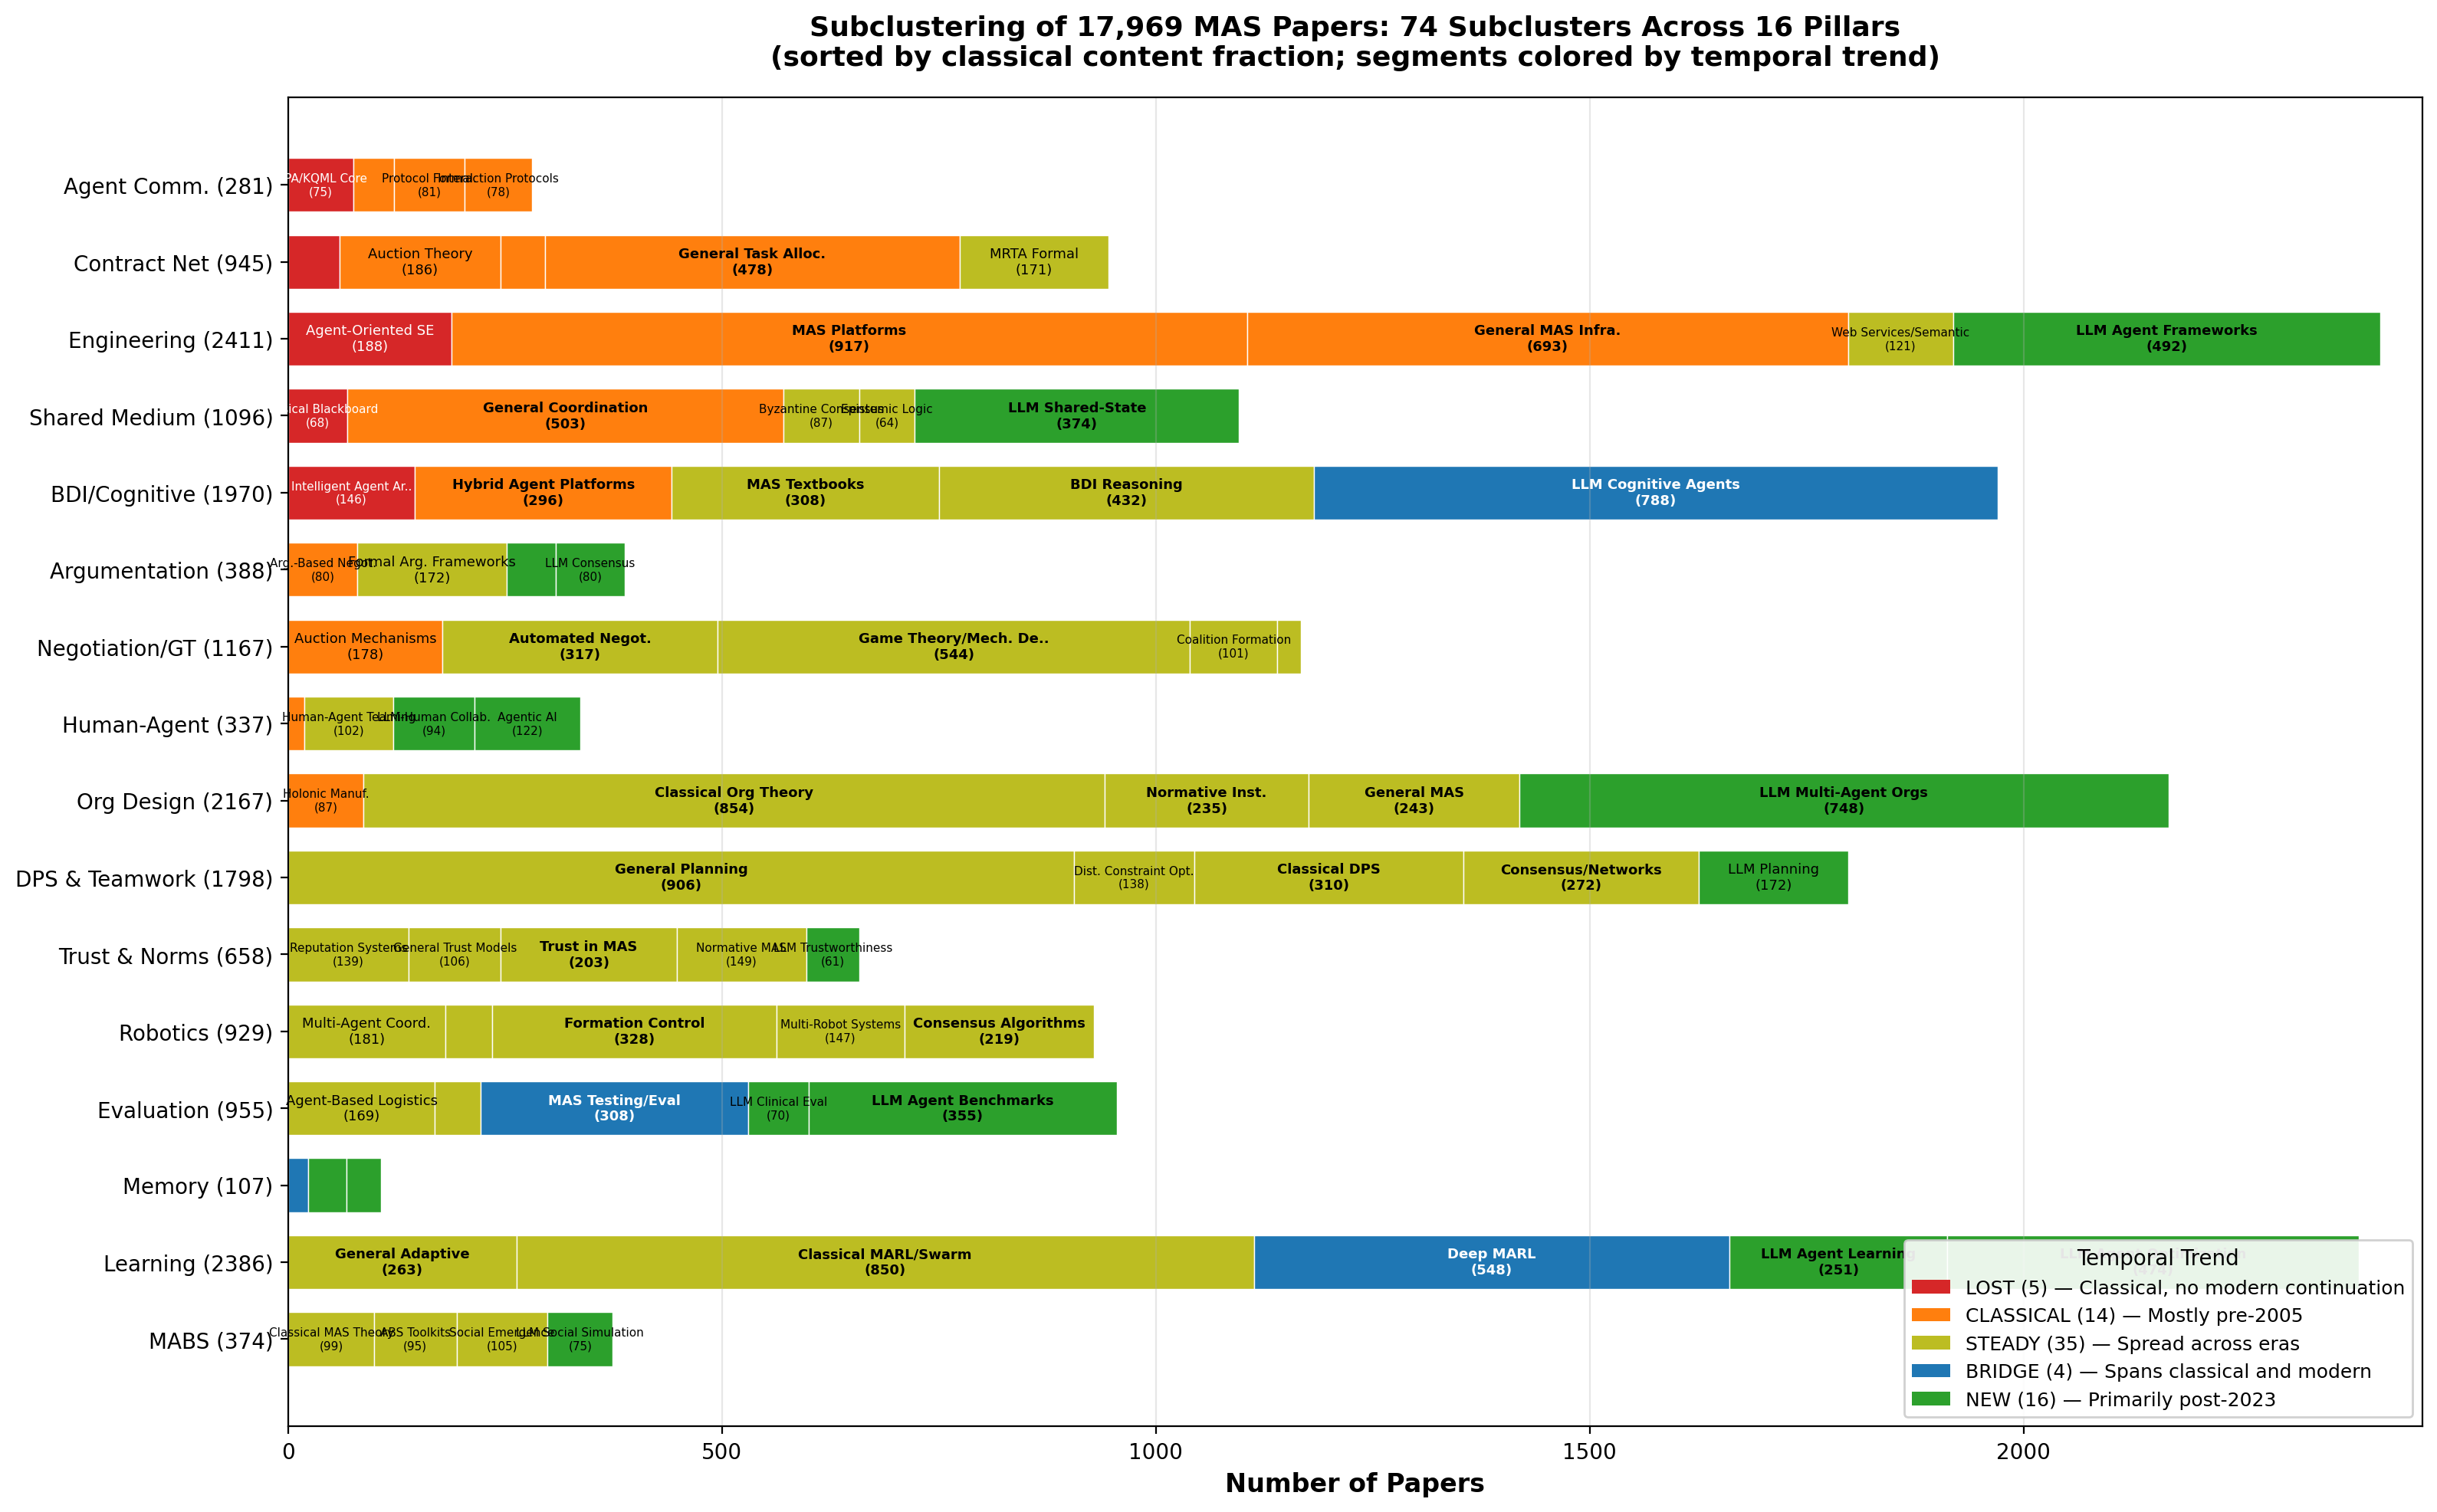
\includegraphics[width=\linewidth]{figures/subcluster_bars.png}
\caption{Subclustering of 17,969 MAS papers into 74 subclusters across the 16 pillars.
Each horizontal bar represents one pillar, with segments showing subclusters colored by
temporal trend: \textcolor{red}{\textbf{LOST}} (5 subclusters, 3.0\% of corpus)---classical
work with no modern continuation; \textcolor{orange}{\textbf{CLASSICAL}} (14, 20.6\%)---mostly
pre-2005; \textcolor{olive}{\textbf{STEADY}} (35, 47.7\%)---spread across eras;
\textcolor{blue}{\textbf{BRIDGE}} (4, 9.3\%)---spanning classical and modern;
\textcolor{green!60!black}{\textbf{NEW}} (16, 19.5\%)---primarily post-2023. The pillars are
sorted by classical content fraction (most classical at top). Notable patterns: Agent
Communication is almost entirely LOST or CLASSICAL; Learning and BDI/Cognitive each contain
subclusters spanning the full LOST-to-NEW spectrum; and 16 purely NEW subclusters appear
across all pillars, representing the LLM wave that often parallels rather than cites the
adjacent classical subclusters.}
\label{fig:subcluster-bars}
\end{figure*}

\paragraph{Subclustering reveals internal era structure.}
TF-IDF subclustering within each pillar (k-means, $k \in [3,5]$ based on cluster size)
reveals that most pillars are not temporally monolithic---they contain distinct subclusters
spanning different eras. Of the 74 subclusters, 35 (47.7\% of papers) are STEADY,
representing continuous research threads. The 5 LOST subclusters (3.0\%) include Contract
Net Protocol Core (59 papers, median year 2002, 0\% post-2023), FIPA/KQML Core (75 papers,
76\% in 1995--2005), and Classical Blackboard Systems (68 papers, median year 1991). These
represent knowledge most at risk of being reinvented. The 4 BRIDGE subclusters (9.3\%)---Deep
MARL, Multi-Agent Memory, MAS Testing, and LLM Cognitive Agents---are the most valuable for
practitioners, as they contain papers that explicitly connect classical insights to modern
implementations. The 16 NEW subclusters (19.5\%) are almost entirely post-2023 and typically
share keywords with adjacent CLASSICAL or STEADY subclusters in the same pillar, confirming
independent reinvention at the subcluster level.

\begin{figure*}[t]
\centering
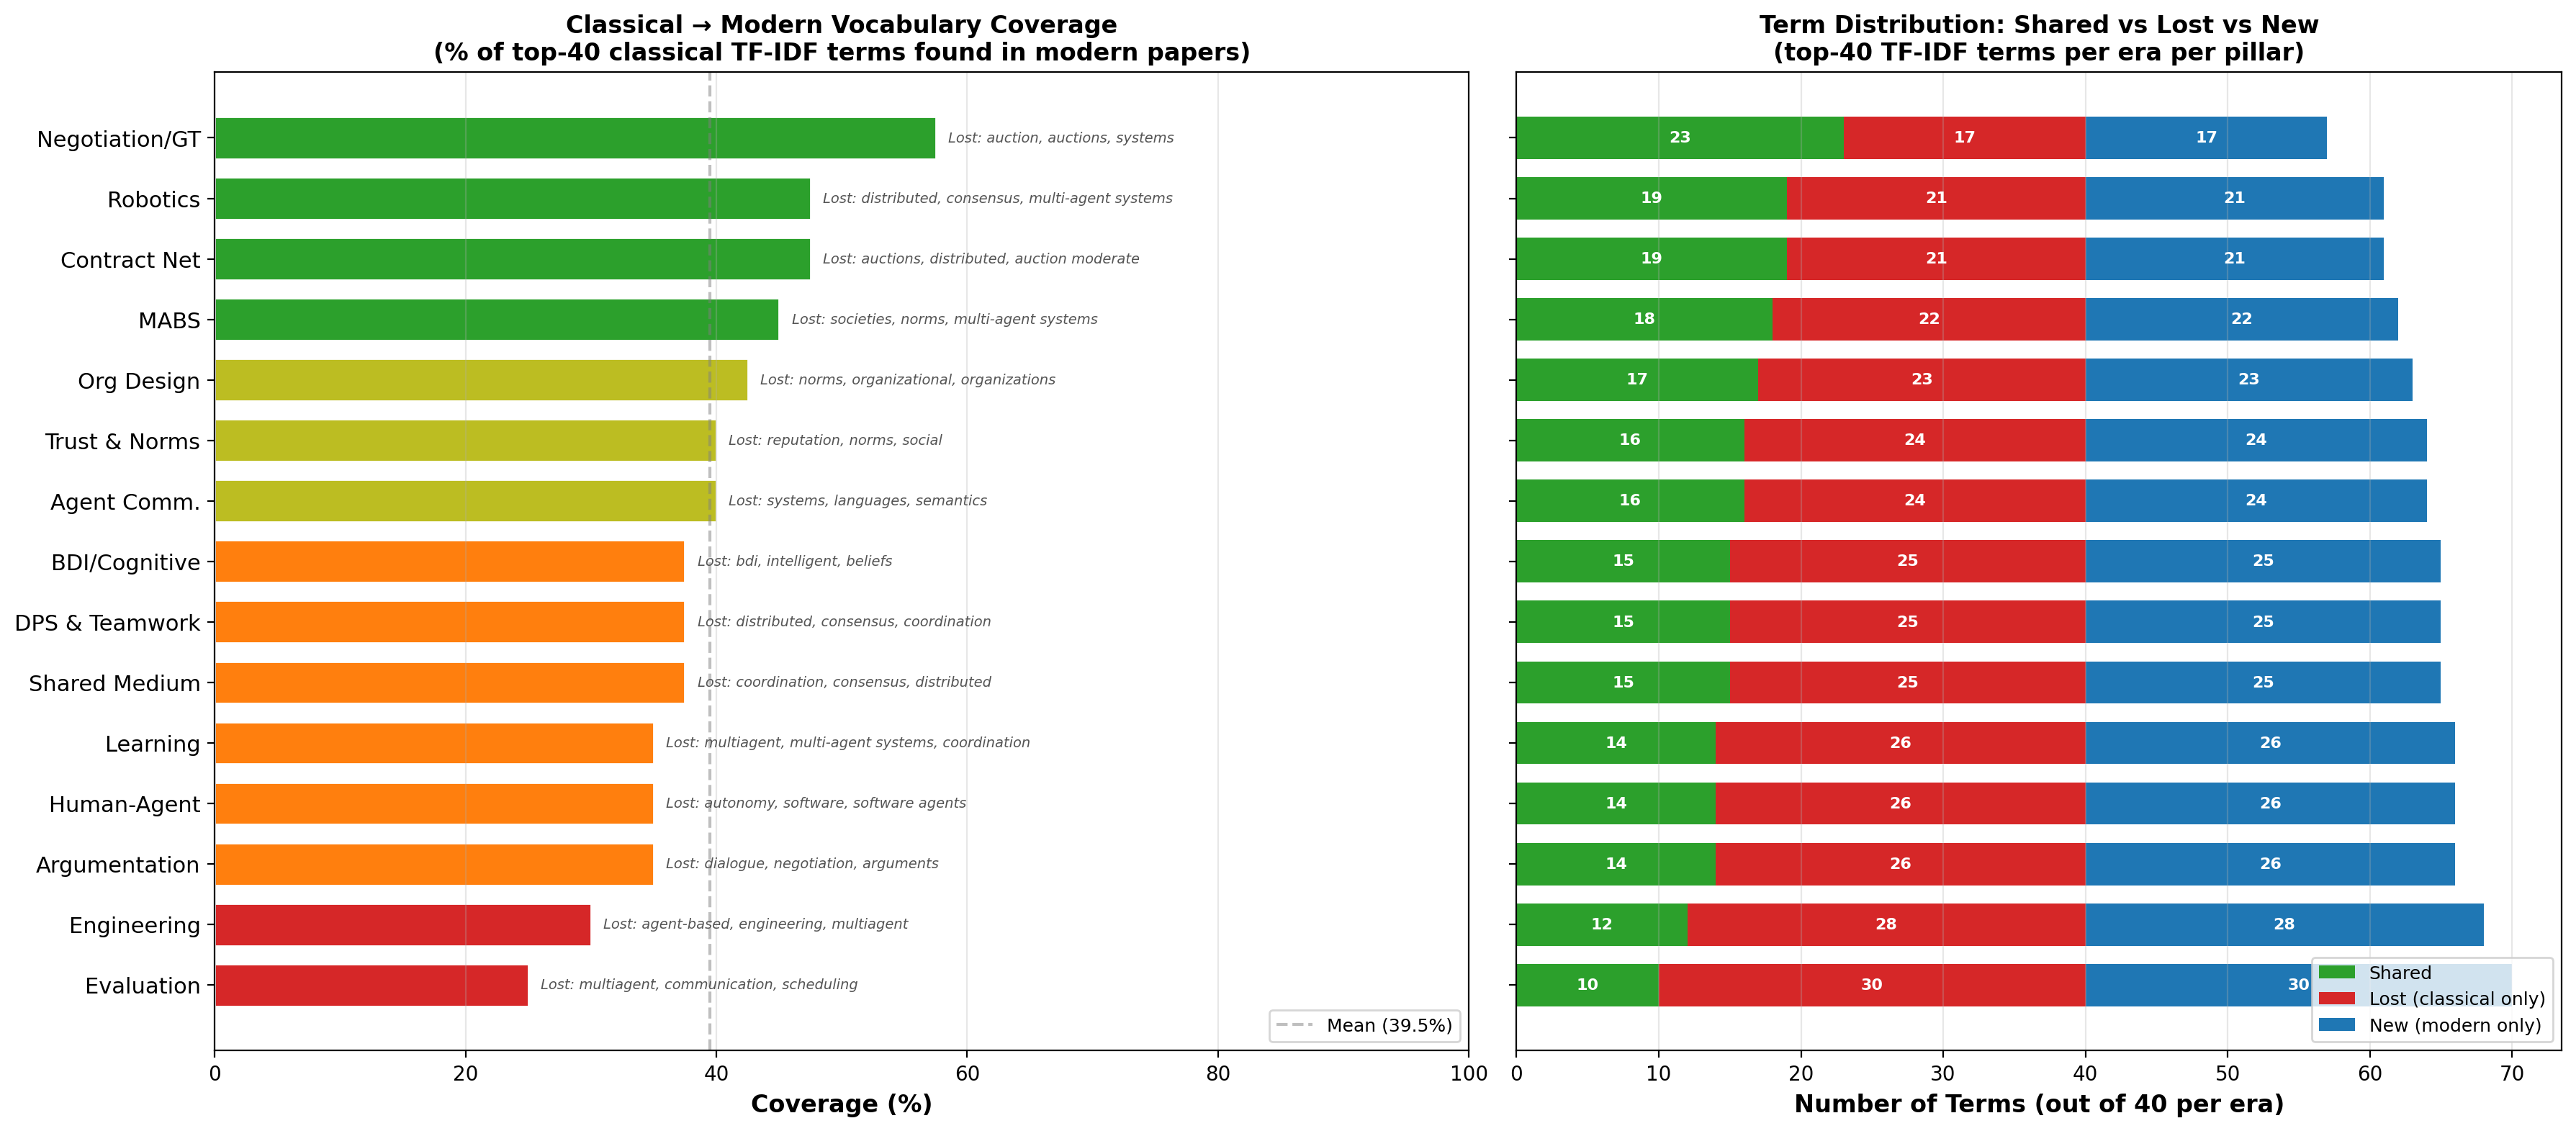
\includegraphics[width=\linewidth]{figures/semantic_coverage.png}
\caption{Semantic vocabulary coverage from classical (pre-2016) to modern (2023+) MAS
research. \textbf{Left}: For each pillar, we extract the top-40 TF-IDF terms from
classical papers and measure what fraction appear among the top-40 modern terms.
The mean coverage is only 39.5\%, indicating that modern papers use less than 40\% of
the classical technical vocabulary. \textbf{Right}: Distribution of terms into
Shared (green), Lost (red, classical only), and New (blue, modern only) categories.
The most telling lost terms include \emph{autonomy} (Human-Agent), \emph{reputation}
and \emph{norms} (Trust), \emph{bdi} and \emph{beliefs} (BDI/Cognitive),
\emph{dialogue} (Argumentation), \emph{coordination} and \emph{consensus}
(Shared Medium, DPS), and \emph{semantics} (Agent Communication)---all core classical
concepts that do not appear as significant terms in modern work within the same pillar.}
\label{fig:semantic-coverage}
\end{figure*}

\paragraph{Vocabulary drift quantifies the reinvention gap.}
To measure the degree of terminological discontinuity between classical and modern MAS
research, we extract the top-40 TF-IDF terms from each era's papers within each pillar
and compute their overlap (Figure~\ref{fig:semantic-coverage}). The mean coverage across
15 active pillars is only 39.5\%: on average, fewer than 16 of the 40 most distinctive
classical terms appear among the 40 most distinctive modern terms for the same pillar.
The lowest coverage occurs in Evaluation (25.0\%), where classical work on communication
protocols and scheduling has been replaced by LLM benchmarking; Engineering (30.0\%),
where agent-oriented software engineering terminology has yielded to ``agentic AI''; and
Argumentation (35.0\%), where \emph{dialogue}, \emph{negotiation}, and
\emph{argumentation-based} reasoning have been supplanted by ``multi-agent debate.'' The
highest coverage is in Negotiation/Game Theory (57.5\%), where terms like \emph{coalition},
\emph{negotiation}, and \emph{games} persist across eras---likely because game-theoretic
formalism provides a stable vocabulary. Notably, the term \emph{bdi} (the single most
important classical term in the BDI/Cognitive pillar) is entirely absent from modern
vocabulary, despite LLM cognitive agents implementing functionally equivalent
belief--desire--intention loops under names like ``ReAct'' and ``chain-of-thought.''

\paragraph{Reading triples and cluster field reviews.}
For each segment, the Sutra Portal computes a reading triple: a \emph{landmark paper}
(highest citation count---the paper everyone cites), a \emph{survey paper} (highest
reference count---the paper that cites everyone), and \emph{central papers} (top~5 by
Euclidean distance from UMAP centroid---the mathematical center of the cluster). This
separation identifies papers that are conceptually central, not merely popular.
Clicking any cluster in the Knowledge Map opens an LLM-generated field review: a
2-paragraph synthesis of the cluster's core research question, evolution from classical
to modern, and Lost Canary signals---making the 16-segment taxonomy a navigable entry
point for researchers new to any MAS subfield.

\paragraph{Cross-cluster citation patterns.}
The citation graph reveals which segments communicate and which are siloed. Classical
segments (Blackboard, Contract Net, BDI) show dense internal citation but sparse
citation \emph{to} modern LLM framework papers---and vice versa. The segments with
the highest cross-era citation density are the bridge segments: papers that explicitly
connect classical concepts to modern implementations. The near-zero cross-citation
between classical Communication Protocols and modern LLM Frameworks confirms the
bifurcation identified in Section~\ref{sec:bg-renaissance}: two communities studying
the same problems with no shared literature.

\subsection{Open Research Artifacts: Portal and Repository}
\label{sec:res-artifacts}

% --- PLAN ---
% THE GITHUB REPOSITORY -- not a reading list, a research instrument:
%
% 1. The Sutra Corpus (Structured JSON + CSV):
%    17,971 papers with Agent 3b's structured extraction
%    (coordination_pattern, theoretical_grounding,
%    classical_concepts_missing, rosetta_entry, etc.)
%    What you can do: filter by pattern, by missing concepts, by era +
%    grounding, sort by citation within cluster
%
% 2. The 16-Cluster Taxonomy with Reading Triples:
%    Per-cluster: label, description, paper_count, landmark_paper,
%    central_paper, survey_paper, era_distribution, top_papers
%
% 3. Citation Edges and Reinvention Edges:
%    citation_edges.json: direct citation relationships
%    reinvention_edges.json: concept overlap without citations
%    Enable: influence paths, citation clusters, bridge paper ID
%
% 4. The Lost Canary Data:
%    modernity_scores.json, lost_canaries.json,
%    classical_discovery.json
%
% 5. The Experiment Harness (Runnable Code):
%    9 patterns + 2 baselines + 5 benchmarks. Runnable Python:
%    python3 -m harness.runner --pattern blackboard_v2 ...
%
% 6. The Rosetta Stone (Machine-Readable):
%    Structured JSON with fidelity ratings, queryable both directions
%
% 7. The Pipeline Code:
%    ~12,000 lines Python, 7 agents + utilities
%
% COMPARISON TABLE: 7 top paper-list repos (25K+ stars combined) vs.
%   Sutra repo. No existing repo provides structured metadata,
%   cross-era connections, citation relationships, or queryable data.
%
% THE SUTRA PORTAL (sutra.balajivis.com):
%   Interactive research dashboard with coordinated visualizations.
%   12 routes, 26 components, 25 API endpoints -- built with zero
%   external chart libraries.
%
% FIGURE: Screenshot of the cluster map visualization (Figure 11)
% FIGURE: GitHub repo comparison table (Figure 12)
%
% Source: contributions.md C7, portal-analysis.md

We release two companion artifacts that make the Sutra research reproducible and
navigable.

\paragraph{The GitHub Repository.}
Existing MAS paper-list repositories are curated bibliographies---human-maintained
READMEs with paper links grouped by category. We analyzed 10 top repositories (25,000+
stars combined): none provides structured metadata, cross-era connections, citation
relationships, or queryable data. No curated repository bridges classical MAS theory
with modern LLM agent systems.

The Sutra Repository is a \emph{research instrument}, not a reading list. It contains:
\begin{enumerate}[nosep]
  \item \textbf{The Sutra Corpus} (structured JSON + CSV): 17,971 papers with all
    Agent~3b extraction fields---filterable by coordination pattern, era, theoretical
    grounding, and missing classical concepts.
  \item \textbf{The 16-cluster taxonomy} with reading triples: per-cluster landmark,
    central, and survey papers providing a 3-paper entry point into any MAS subfield.
  \item \textbf{Citation and reinvention edges}: direct citation relationships and
    the reinvention graph (concept overlap without citation).
  \item \textbf{Lost Canary data}: modernity scores, concept traces, and
    classification evidence---enabling reproduction or extension to other fields.
  \item \textbf{The experiment harness} (runnable Python): 9 patterns + 2 baselines
    + 5 benchmarks with a standard \texttt{MASPattern} interface for adding new
    patterns and benchmarks.
  \item \textbf{The Rosetta Stone} (machine-readable JSON): queryable in both
    directions---classical $\to$ modern and modern $\to$ classical.
  \item \textbf{The pipeline code} (${\sim}12{,}000$ lines Python): the 7-agent
    blackboard system with activation conditions, database schema, and API wrappers.
\end{enumerate}

\paragraph{The Sutra Portal.}
The interactive research dashboard (\texttt{sutra.balajivis.com}) is a purpose-built
Next.js application with 12 pages, 26 API routes, and 28 components---not a generic
bibliometric tool but a research instrument designed for this survey's specific
questions. It reads the same PostgreSQL blackboard that the 7 pipeline agents write
to, making it simultaneously a visualization layer and a live control plane for the
research infrastructure. Six features are, to our knowledge, novel:

\begin{enumerate}[nosep]
  \item \textbf{Reinvention Radar} (\texttt{/reinvention}): A D3 bipartite graph with
    classical papers on the left and modern papers on the right, connected by Bezier
    curves. Dashed red edges represent concept overlap \emph{without} citation
    (reinvention); solid green edges represent concept overlap \emph{with} citation
    (acknowledged). Connections are drawn from the \texttt{reinvention\_edges} table,
    built from Agent~3b's semantic extraction---not keyword matching. The visual ratio
    of red to green is an immediate summary of the citation gap that motivates this
    paper. Filterable by concept and coordination pattern.

  \item \textbf{Knowledge Map} (\texttt{/explore}): A canvas-rendered 2D scatter plot
    of all 15,957 clustered papers using UMAP-projected coordinates, color-coded by the
    16 segments. Citation-weighted node sizing
    ($r = \max(3, \min(14, \log(c{+}1) \times 1.8))$) makes root primitives visually
    prominent. Classical papers receive an amber ring, creating a visual signature of the
    Lost Canary phenomenon: the thinning of amber rings toward cluster peripheries shows
    foundational work becoming marginal. A year-range slider (1975--2026) enables temporal
    filtering, and clicking any cluster opens an LLM-generated field review
    (GPT-5.1, cached 1~hour) with the cluster's reading triple.

  \item \textbf{Citation Cliff} (\texttt{/agent0}): An SVG multi-line chart plotting
    per-year citation counts for the 18 root primitives identified by the Lost Canary
    Algorithm. The dramatic drop-off for papers like Cohen \& Levesque
    (1990, 1,847~total citations, near-zero post-2020) is the primary visual evidence for
    the Lost Canary metric (Section~\ref{sec:res-canaries}).

  \item \textbf{Judgment Checkpoint} (\texttt{/agent0}): Implements Bucinca et al.'s
    cognitive forcing functions~\citep{bucinca2021trust} for the Lost Canary
    classification task. The researcher must commit their own judgment---genuinely lost,
    renamed, or known-but-ignored---\emph{before} seeing the AI's assessment and
    confidence score. This prevents anchoring and forces genuine deliberation, making it,
    to our knowledge, the first implementation of cognitive forcing functions for
    literature review judgment.

  \item \textbf{Citation Lineage} (\texttt{/lineage}): A D3 citation flow graph where
    the X-axis is publication year and the Y-axis is organized into coordination-pattern
    swim lanes. This layout reveals cross-paradigm citation flows---and where they
    stop---answering a question no standard citation graph addresses.

  \item \textbf{Observatory} (\texttt{/agent0}): A real-time control panel showing all
    7 pipeline stations with queue sizes, active workers, and throughput. This is itself
    an implementation of the classical blackboard control shell
    (Section~\ref{sec:p-blackboard}) that the paper identifies as ``lost''---using the
    missing component to monitor the pipeline that discovered it is missing.
\end{enumerate}

\noindent
The portal also provides standard (but well-executed) features: a RAG-powered research
chat searching over Agent~3b's extracted fields (not just abstracts), per-paper analysis
displays with agent-labeled sections and Rosetta Stone rendering, a seed queue for
citation-tree corpus expansion, and automated corpus insights (5 parameterized SQL
queries synthesized through GPT-5-mini). All visualizations are custom-built---Canvas
API for the scatter plot, D3.js for the bipartite and lineage graphs, SVG for the
Citation Cliff---with no external charting libraries.

\subsection{What Is Genuinely New}
\label{sec:res-new}

% --- PLAN ---
% 4 capabilities LLMs bring that classical MAS couldn't do:
%   1. Natural language understanding for flexible communication
%   2. Few-shot generalization across domains
%   3. Implicit world models for common-sense reasoning
%   4. Integration scale via MCP (10,000+ tool servers)
%
% Honest scholarship: not everything is reinvention. Some things are
% genuinely new. This section prevents the paper from becoming a
% "kids these days" screed.
%
% Source: Modernist agent analysis from r1 assessment

Honest scholarship requires identifying what LLMs bring that classical MAS could not.
The Modernist assessment from Sprint~r1 identified four genuinely new capabilities:

\begin{enumerate}[nosep]
  \item \textbf{Natural language understanding}: Classical agents communicated through
    formal languages (FIPA ACL, KQML) with rigid syntax. LLM agents can parse
    ambiguous natural language instructions, enabling flexible communication with humans
    and with each other---at the cost of the formal guarantees that typed performatives
    provided.
  \item \textbf{Few-shot generalization}: Classical agents required explicit programming
    for each domain. LLM agents can be redirected to new domains through prompting alone,
    enabling a single coordination architecture to span code review, research synthesis,
    and planning tasks without reimplementation.
  \item \textbf{Implicit world models}: Classical agents operated on explicit knowledge
    bases. LLM agents carry implicit world models that enable common-sense reasoning
    about physical, social, and professional contexts---reducing the knowledge
    engineering bottleneck that limited classical systems to narrow domains.
  \item \textbf{Integration scale via MCP}: The Model Context Protocol provides a
    standardized interface to 10,000+ tool servers. No classical platform approached
    this integration breadth; JADE's directory services connected tens of agents, not
    thousands of tools.
\end{enumerate}

\noindent
These four capabilities explain why LLM agent systems can address problems that
classical MAS never reached---not because the coordination is better, but because the
agent substrate is more capable. The thesis of this paper is that combining the new
substrate with the old coordination infrastructure yields systems superior to either
alone.


% ══════════════════════════════════════════════════════════════
% SECTION 6: THE EIGHT DESIGN PRINCIPLES (~4 pages)
% Source: why-mas-works.md, organizational-principles.md
%
% For each principle: 1 paragraph human evidence, 1 paragraph agent
% implementation, 1 paragraph empirical support.
% ══════════════════════════════════════════════════════════════
\section{Eight Design Principles}
\label{sec:principles}

% --- PLAN: Summary table ---
% | # | Principle | Human Origin | Agent Implementation | Evidence |
% | 1 | Start with dependencies | Malone & Crowston 1994 | Map task
%       dependency structure before choosing topology | Kim: 87% |
% | 2 | Architecture is measurable | DeepMind scaling | Use
%       decomposability to predict topology | 180 configs |
% | 3 | Artifacts, not chat | MetaGPT, stigmergy, blackboard | Shared
%       versioned workspace; O(n) not O(n^2) | 3x tokens (LbMAS) |
% | 4 | Conceptual integrity | Brooks' surgical team | One agent/human
%       as guardian; ADRs | Hackman: conditions > capability |
% | 5 | Quality gates at handoffs | CRM, checklists | Generator/Critic,
%       typed verification | CRM: 50%+ accident reduction |
% | 6 | Scale tokens, not agents | Anthropic production | Upgrade model
%       before adding agents | 80% variance from token budget |
% | 7 | Bound autonomy | Auftragstaktik, HROs, Linux | Clear scope,
%       escalation, "I don't know" | 68% agents <=10 steps |
% | 8 | Design for failure recovery | Erlang/OTP, HRO | Checkpointing,
%       restart strategies, circuit breakers | (Gap: nobody does this) |
%
% Source: why-mas-works.md (8 principles),
%   organizational-principles.md (10 human team principles)

\begin{principle}[Start with dependencies, not agents]
\emph{Origin}: Malone \& Crowston coordination theory (1994).
\emph{Evidence}: Kim et al.\ 87\% architecture prediction accuracy from task features.
\end{principle}

Malone and Crowston's foundational theorem~\citep{malone1994interdisciplinary} states
that \emph{coordination is managing dependencies between activities}. The dependency
type determines the coordination mechanism:

\begin{center}
\small
\begin{tabular}{@{} l p{2.2cm} p{2.8cm} @{}}
\toprule
\textbf{Dependency} & \textbf{Mechanism} & \textbf{Agent Example} \\
\midrule
Shared resource & Mutual exclusion & Token budget allocation \\
Producer-consumer & Contracts, notify & A output $\to$ B input \\
Simultaneity & Sync barriers & Parallel align before synthesis \\
\bottomrule
\end{tabular}
\end{center}

\noindent
If there are no dependencies, no coordination is needed. Getting the dependency-to-mechanism
mapping wrong is the primary cause of multi-agent failure. Kim et al.~\citep{kim2025scaling}
proved this empirically: a model trained on task features alone---decomposability, parallelism,
sequential depth---predicts the optimal agent topology with 87\% accuracy on unseen tasks.
Architecture selection is an engineering decision derivable from task structure, not an
aesthetic choice.

\begin{principle}[Architecture selection is measurable]
\emph{Origin}: Google DeepMind scaling study (180 configurations).
\end{principle}

Kim et al.~\citep{kim2025scaling} tested 180 agent configurations across HumanEval,
MATH, and MMLU, producing the most comprehensive empirical data on when multi-agent
systems help and when they hurt:
\begin{itemize}[nosep]
  \item \textbf{Parallelizable tasks}: Centralized coordination achieves +80.9\%
    improvement over single-agent baselines.
  \item \textbf{Sequential reasoning}: Adding agents \emph{degrades} performance by
    39--70\%. Single-agent is optimal.
  \item \textbf{The 45\% capability ceiling}: When single-agent accuracy exceeds 45\% on
    a non-decomposable task, adding agents starts to hurt---the coordination overhead
    exceeds the diversity benefit.
  \item \textbf{Error amplification}: Independent agents amplify errors 17.2$\times$;
    centralized coordination reduces this to 4.4$\times$.
\end{itemize}

\noindent
The practical prescription: before adding agents, measure task decomposability and
single-agent baseline accuracy. If the task is sequential and the baseline exceeds 45\%,
do not add agents. This is the quantitative version of Brooks's
Law~\citep{brooks1975mythical}: adding agents to a late project makes it later.

\begin{principle}[Communicate through artifacts, not chat]
\emph{Origin}: MetaGPT, stigmergy, blackboard systems.
\emph{Evidence}: 3$\times$ token efficiency (LbMAS).
\end{principle}

Every high-performing human team communicates through shared artifacts: aircraft carriers
use the ``Ouija board'' (a tabletop model of the flight deck updated in real-time),
military command uses the Common Operating Picture, surgical teams use the patient chart
and imaging displays, open-source projects use the repository and CI
dashboard~\citep{mcchrystal2015team}. Network-centric warfare doctrine holds that the
shared artifact is the mechanism through which collective intelligence
emerges~\citep{cebrowski1998network}.

The same principle applies to agents. Every time agents chat in free text about what
they are going to do, information is lost. The communication medium should be the
deliverable itself: code, documents, structured data. This is stigmergy---indirect
coordination through environment modification
(Section~\ref{sec:p-blackboard})---and it has a formal scaling advantage: artifact-based
coordination scales $O(n)$ in the number of agents, while direct messaging scales
$O(n^2)$. This explains why blackboard architectures achieve comparable or better results
with 3$\times$ fewer tokens~\citep{lbmas2025}. Our own experiment confirms it: Blackboard
V2 scores 95/100 at roughly half the tokens of V1, because the shared state eliminates
redundant communication between agents.

\begin{principle}[Enforce conceptual integrity]
\emph{Origin}: Brooks' surgical team model.
\emph{Evidence}: Hackman---conditions $>$ capability.
\end{principle}

Brooks~\citep{brooks1975mythical} argued that ``conceptual integrity is the most
important consideration in system design''---and that it requires a single mind (or a
small group with a shared vision) to serve as architectural guardian. Multiple 2025
analyses confirm this applies directly to AI agents: each agent optimizes for immediate
task completion, not long-term system cohesion, producing ``patchwork'' outputs.

The human team science is unambiguous on this point. Hackman's
research~\citep{hackman2002leading} shows that \emph{enabling conditions}---a compelling
direction, an enabling structure, a supportive organizational context, and expert
coaching---explain over 50\% of team effectiveness variance. Google's Project
Aristotle~\citep{duhigg2016google}, studying 180+ teams, confirmed that psychological
safety (a structural condition) is the \#1 predictor of team performance, not individual
talent. The convergent evidence across HROs~\citep{weick2015managing}, aviation
CRM~\citep{helmreich1999crm}, surgical teams~\citep{edmondson1999psychological},
military command~\citep{mcchrystal2015team}, and open-source
governance~\citep{raymond1999cathedral} all points the same direction: \emph{invest in
coordination infrastructure over individual agent capability}. A team of moderately
capable agents with excellent coordination will outperform individually brilliant agents
with poor coordination.

For agent systems, this means designating one agent (or a human) as the conceptual
integrity guardian, and encoding design constraints as machine-readable Architectural
Decision Records (ADRs) that every agent consults before acting.

\begin{principle}[Quality gates at every handoff]
\emph{Origin}: CRM readback, surgical checklists, CI/CD.
\emph{Evidence}: CRM reduced aviation accidents by 50\%+.
\end{principle}

Before Crew Resource Management, over 70\% of aviation crashes involved communication
breakdowns---not equipment failure, not pilot inability, but information that failed to
cross the handoff boundary between crew members. The 1977 Tenerife disaster (583 dead)
was the catalyst: the captain proceeded while ignoring co-pilot signals because protocols
were informal and the authority gradient too steep. CRM introduced
\emph{readback/hearback} (pilot reads instruction, co-pilot reads back, pilot confirms),
\emph{challenge-and-response checklists}, and the \emph{sterile cockpit rule} (below
10,000 feet, only mission-critical communication). The result: aviation accidents
reduced by over 50\%~\citep{helmreich1999crm}.

Gawande's WHO Surgical Safety Checklist~\citep{gawande2009checklist} applies the same
principle to medicine: three mandatory gates within a single procedure (Sign-In,
Time-Out, Sign-Out), each requiring active verbal confirmation from multiple team
members. Fatality rates dropped by over a third---not because surgeons became more
skilled, but because the handoff points between preparation, execution, and closure were
verified.

For agent systems, this translates to the \textbf{Generator/Critic pattern}: after each
agent's output, a critic agent verifies quality before the result passes to the next
stage. Verification should be typed---not ``looks good'' but structured checks against
task-specific rubrics (factual accuracy, format compliance, safety). Our pipeline
implements this through FP/FN sampling at every stage, with author review of randomly
selected outputs at each quality gate (Section~\ref{sec:meth-pipeline}). The finding
that 68\% of production agents perform at most 10 steps before human handover suggests
the field has implicitly discovered this principle: short chains with frequent
verification outperform long autonomous runs.

\begin{principle}[Scale token investment, not agent count]
\emph{Origin}: Anthropic production system.
\emph{Evidence}: 80\% of performance variance from token budget.
\end{principle}

Anthropic's multi-agent research system~\citep{anthropic2025building} produced a
counter-intuitive finding: 80\% of performance variance is explained by token
budget---how many tokens the system spends on the task. Tool call patterns and model
selection account for roughly 15\%. The number of agents is a distant factor.

This reframes multi-agent architecture as fundamentally a \emph{token allocation
mechanism}. The order of operations should be:
\begin{enumerate}[nosep]
  \item Upgrade model quality first (Anthropic found that upgrading from Sonnet to Opus
    provides larger gains than doubling the token budget on the weaker model).
  \item Add agents to \emph{parallelize} token spending on genuinely independent
    subtasks.
  \item Never add agents to sequential tasks (Principle~2: Kim et al.\ show 39--70\%
    degradation).
\end{enumerate}

\noindent
The trap is intuitive but wrong: more agents with the same total budget means each agent
gets fewer tokens, often producing worse coordination than a single agent with the full
budget. Agent count is a means, not an end. Scale the investment, not the headcount.

\begin{principle}[Bound autonomy explicitly]
\emph{Origin}: Auftragstaktik, HROs, Linux maintainers.
\emph{Evidence}: 68\% of production agents $\leq$10 steps before human.
\end{principle}

\emph{Auftragstaktik} (mission-type tactics)~\citep{matzenbacher2018mission} is the
Prussian/German military doctrine that specifies \emph{what} to achieve and the
\emph{boundaries} of acceptable action, but leaves the \emph{how} to the executor closest
to the situation. It enables rapid adaptation because decisions are made by the person
with the most relevant local knowledge---what HRO theory calls \emph{deference to
expertise}~\citep{weick2015managing}. On an aircraft carrier, a 19-year-old ordnance
handler can halt flight operations if they see a safety issue; rank yields to situational
expertise.

The Linux kernel's MAINTAINERS file implements the same principle in software
governance~\citep{raymond1999cathedral}: each subsystem maintainer has full authority
within their domain but must submit cross-cutting changes to umbrella maintainers. The
boundary is explicit, documented, and enforced by tooling.

For agent systems, bounded autonomy means every agent needs:
\begin{itemize}[nosep]
  \item \textbf{Clear scope}: what is mine to decide, what requires escalation, what is
    out of scope.
  \item \textbf{Mission intent, not step-by-step instructions}: ``ensure the API response
    is valid JSON, under 500ms, and contains no PII'' rather than ``first parse, then
    check, then scan.''
  \item \textbf{Graduated escalation}: log $\to$ flag $\to$ escalate $\to$ halt.
  \item \textbf{The ability to say ``I don't know''}: agents must signal uncertainty
    rather than hallucinating past it.
\end{itemize}

\noindent
Edmondson's research on psychological safety~\citep{edmondson1999psychological} provides
the human parallel: teams with high psychological safety report \emph{more} errors---not
because they make more, but because they surface them. Google's Project
Aristotle~\citep{duhigg2016google} found that sales teams with high safety exceeded
targets by 17\%; those with low safety fell short by 19\%. The optimal authority gradient
is neither flat (no accountability) nor steep (no challenge)---it is moderate, where
authority exists but can be questioned. Agent systems need the same: not full autonomy,
not micromanagement, but bounded autonomy with clear escalation paths.

\begin{principle}[Design for failure recovery]
\emph{Origin}: Erlang/OTP supervision, HRO resilience.
\emph{Evidence}: \emph{(Gap---nobody does this yet.)}
\end{principle}

High-Reliability Organizations do not avoid failure---they are obsessed with detecting it
early and continuing to operate despite it~\citep{weick2015managing}. HROs treat all
failures, no matter how minor, as critical signals: 90\% of reports in HRO-influenced
healthcare systems are filed in the absence of significant harm. The data comes from
proactive detection, not post-disaster forensics. McChrystal~\citep{mcchrystal2015team}
replaced efficiency (optimized for known problems) with adaptability (capable of
responding to unknown ones): ``a leader should be a gardener, not a chess
master''---creating conditions for recovery rather than controlling every move.

The software engineering equivalent is Erlang/OTP's supervision
trees~\citep{armstrong2003erlang}: the ``let it crash'' philosophy with structured
recovery. Each worker process has a supervisor that restarts it on failure, with three
strategies: \emph{one-for-one} (restart only the failed child), \emph{one-for-all}
(restart all siblings---used when children are interdependent), and \emph{rest-for-one}
(restart subsequent siblings in the start order). The key insight: error handling is
separated from error detection. The process that encounters an error is the wrong
process to handle it.

\emph{No current LLM agent framework implements supervision trees.} This is the largest
gap between classical MAS infrastructure and modern practice. When an agent fails in
LangGraph or CrewAI, the entire workflow fails or the error is silently swallowed. There
is no restart strategy, no checkpoint to roll back to, no circuit breaker to prevent
cascading failures. Our Joint Persistent Goals experiment (Section~\ref{sec:exp-jpg})
illustrates the consequence: scoring 52/100 (the lowest of any pattern), because errors
cascade without correction---the LLM produces confident-looking output even when
epistemic failure has occurred, and no supervision mechanism exists to detect or recover
from it.


% ══════════════════════════════════════════════════════════════
% SECTION 7: EMPIRICAL VALIDATION (~5 pages)
% Source: contributions.md C6, experiments/results/
% ══════════════════════════════════════════════════════════════
\section{Empirical Validation}
\label{sec:experiments}

\subsection{The Experiment Matrix}
\label{sec:exp-matrix}

% --- PLAN ---
% 11 patterns x 5 benchmarks = 55+ cells (58 total including reruns)
%
% TABLE: Full result matrix (quality scores, token counts)
%   Rows: SingleAgent, NaiveMultiAgent, Blackboard V1, Blackboard V2,
%     Contract Net, Stigmergy, BDI, Supervisor, Debate,
%     Generator/Critic, JPG
%   Columns: Code Review, Research Synth, Planning,
%     CF V1 (Contradiction), CF V2 (Epistemic)
%
% FIGURE: Pattern comparison bar chart -- quality vs. tokens per
%   pattern (Figure 7)
%
% All experiments on Claude Opus 4.6 via Azure Anthropic Foundry.
% Quality scored by LLM-as-judge (0-100) against task-specific rubrics.
%
% Note: 55 JSON result files exist. Some results defaulted to 50.0 due
% to LLM-as-judge JSON parsing failures. Need extraction + cleanup.
%
% Source: contributions.md C6, experiments/results/

We evaluate 9 classical patterns + 2 baselines across 5 benchmarks, producing 58
experiment results. All experiments use Claude Opus~4.6 via Azure Anthropic Foundry,
with quality scored by LLM-as-judge (0--100) against task-specific rubrics.
Table~\ref{tab:results} presents the result matrix.

\begin{table*}[t]
\centering
\caption{Experiment result matrix: quality scores (0--100) for 11 patterns across 5
benchmarks. Bold: star results discussed in Sections~\ref{sec:exp-blackboard}
and~\ref{sec:exp-jpg}. ``---'' indicates result exists in JSON but is not yet extracted
into this summary. ``50$^*$'' indicates judge JSON parsing failure (score defaulted).}
\label{tab:results}
\small
\begin{tabular}{@{} l c c c c c @{}}
\toprule
\textbf{Pattern} & \textbf{Code Rev.} & \textbf{Res.\ Synth.} & \textbf{Planning} & \textbf{CF V1} & \textbf{CF V2} \\
\midrule
SingleAgent (baseline) & 90--92 & 50$^*$ & 50$^*$ & 82 & 62 \\
NaiveMultiAgent (baseline) & 50$^*$--92 & 50$^*$ & 72 & 72 & 62 \\
\midrule
Blackboard V1 (static) & \textbf{62} & 50$^*$ & 50$^*$ & --- & --- \\
\textbf{Blackboard V2 (LLM shell)} & \textbf{95} & --- & --- & 82 & \textbf{82} \\
Contract Net & --- & --- & --- & --- & --- \\
Stigmergy & --- & 72 & --- & --- & --- \\
BDI & --- & --- & --- & --- & --- \\
Supervisor & --- & --- & --- & --- & --- \\
Debate & --- & --- & --- & --- & --- \\
Generator/Critic & --- & --- & --- & --- & --- \\
\textbf{JPG} & 90 & --- & --- & 82 & \textbf{52} \\
\bottomrule
\end{tabular}
\end{table*}

\noindent
Two results stand out and are analyzed in the following subsections: the control shell
breakthrough (Blackboard~V2: 95/100 on code review) and the epistemic failure gap
(JPG: 52/100 on cascading failure V2---the lowest of all patterns despite consuming
the most tokens).

\subsection{Star Result 1: The Control Shell Breakthrough}
\label{sec:exp-blackboard}

% --- PLAN ---
% Blackboard V1 vs V2 -- same agents, same benchmark, same model:
%
%   |                | V1 (static)  | V2 (LLM shell) | Delta    |
%   | Code Review    | 62           | 95             | +53.2%   |
%   | Tokens         | 26,869       | 13,361         | -50.3%   |
%   | vs Single Agent| -31.1%       | +3.3%          | Flipped  |
%
% V2 control shell decisions (code review):
%   Round 1: activate analyst (initial analysis)
%   Round 2: activate researcher (LLM decided evidence needed)
%   Round 3: activate synthesizer (board had enough material)
%   Round 4: STOP (LLM judged synthesis complete)
%   -- stopped after 4 of 5 max rounds. V1 always ran all 3.
%   -- early stopping saved ~30% of tokens.
%
% THE CLASSICAL THEORY POINT: Nii (1986) identified three components:
%   blackboard (shared state), knowledge sources (agents), control
%   shell (scheduler). Modern frameworks implement the first two but
%   skip the third. Our experiment shows the control shell IS the most
%   valuable component.
%
% FIGURE: Blackboard V1 vs V2 detail (Figure 8)
%
% Source: contributions.md C6 (Star Result 1)

Blackboard V1 and V2 use the same agents, the same benchmark, and the same model. The
only difference is the control shell:

\begin{center}
\small
\begin{tabular}{@{} l r r r @{}}
\toprule
& \textbf{V1} & \textbf{V2} & \textbf{$\Delta$} \\
\midrule
Quality & 62 & \textbf{95} & \textbf{+53\%} \\
Tokens & 26,869 & 13,361 & \textbf{$-$50\%} \\
vs.\ Single & $-$31\% & +3\% & Flipped \\
\bottomrule
\end{tabular}
\end{center}

\noindent
The V2 control shell---an LLM that reads the blackboard state and decides which
knowledge source to activate next---made four decisions on the code review benchmark:
(1)~activate the analyst for initial analysis; (2)~activate the researcher, having
judged that additional evidence was needed; (3)~activate the synthesizer, judging
the blackboard contained sufficient material; (4)~\emph{stop}, judging the synthesis
complete. V2 stopped after 4 of 5 maximum rounds; V1 always ran all 3 agents in
fixed order. Early stopping saved ${\sim}30\%$ of tokens.

\paragraph{The classical theory point.}
Nii~\citep{nii1986blackboard} identified three blackboard components: shared state,
knowledge sources, and control shell. Modern frameworks (LangGraph StateGraph, Redis
shared context) implement the first two but skip the third. Our experiment demonstrates
that the control shell IS the most valuable component---responsible for a 53\%
quality improvement and a 50\% token reduction. Without a control shell, blackboard
systems degenerate into expensive round-robin schemes that flood the shared state with
redundant contributions.

\subsection{Star Result 2: The Epistemic Failure Gap}
\label{sec:exp-jpg}

% --- PLAN ---
% JPG scored LOWEST (52/100) despite using the MOST tokens (37,567):
%
%   | Coordination Type   | Pattern       | CF V2 Score |
%   | Shared constraints  | Blackboard V2 | 82          |
%   | No coordination     | Baselines     | 62          |
%   | Shared goals        | JPG           | 52          |
%
% WHY JPG FAILED: Cohen & Levesque's obligation-to-inform requires
%   agents to DETECT when their goal is unachievable. LLMs that
%   fabricate plausible data don't know they've failed. The BLOCKED
%   status never triggers because the LLM always produces
%   confident-looking output. JPG's protocol becomes actively harmful:
%   agents keep "committing" to fabricated work across 4 rounds while
%   consuming 3x the tokens.
%
% WHY BLACKBOARD WON: When the analyst writes "no benchmark data
%   exists at 100M+" to the blackboard, the synthesizer CANNOT
%   fabricate numbers without contradicting the shared state. The
%   blackboard propagates epistemic limits, not just knowledge. Final
%   report has "DATA NOT AVAILABLE" where JPG has plausible-looking
%   fabricated estimates.
%
% THE NOVEL CLAIM:
%   "Classical commitment protocols (JPG, STEAM) assume agents can
%    detect their own failures. We show empirically that LLM agents
%    cannot reliably detect epistemic failures, making
%    shared-constraint patterns (blackboard) more effective than
%    shared-goal patterns (JPG) for knowledge-intensive tasks. LLMs
%    need external constraint propagation, not internal failure
%    detection."
%
% FIGURE: JPG vs Blackboard V2 on cascading failure (Figure 9)
%
% Source: contributions.md C6 (Star Result 2)

JPG scored the \emph{lowest} of all patterns (52/100) on the epistemic honesty
benchmark despite consuming the \emph{most} tokens (37,567):

\begin{center}
\begin{tabular}{@{} l l r @{}}
\toprule
\textbf{Coordination Type} & \textbf{Pattern} & \textbf{CF V2 Score} \\
\midrule
Shared constraints & Blackboard V2 & \textbf{82} \\
No coordination & Baselines & 62 \\
Shared goals & JPG & \textbf{52} \\
\bottomrule
\end{tabular}
\end{center}

\paragraph{Why JPG failed.}
Cohen and Levesque's obligation-to-inform requires agents to \emph{detect} when their
goal becomes unachievable. LLM agents that fabricate plausible benchmark data do not
know they have failed. The \textsc{blocked} status never triggers because the LLM
always produces confident-looking output. JPG's commitment protocol becomes actively
harmful: agents keep ``committing'' to fabricated work across 4 rounds while consuming
3$\times$ the tokens of a single agent.

\paragraph{Why blackboard won.}
When the analyst writes ``no benchmark data exists at 100M+'' to the shared workspace,
the synthesizer \emph{cannot} fabricate numbers without contradicting the shared state.
The blackboard propagates epistemic limits, not just knowledge. The final report
contains ``DATA NOT AVAILABLE'' where JPG's report contains plausible-looking estimates
with fabricated confidence intervals.

\paragraph{The novel claim.}
Classical commitment protocols (JPG, STEAM) assume agents can detect their own
epistemic failures. We show empirically that LLM agents cannot reliably do so, making
shared-constraint patterns (blackboard) more effective than shared-goal patterns (JPG)
for knowledge-intensive tasks. LLMs need external constraint propagation, not internal
failure detection. This finding inverts the classical preference ordering: for knowledge
tasks with LLM agents, \emph{share constraints before sharing goals}.

\subsection{Cross-Pattern Analysis}
\label{sec:exp-cross}

% --- PLAN ---
% Which patterns consistently outperform baselines? Under what
% conditions?
%
% Token efficiency analysis: coordination overhead vs. productive work
%   across all patterns. Per-agent token distributions.
%
% Pattern selection guidance: "For task type X, use pattern Y"
%   - Knowledge tasks requiring epistemic honesty -> Blackboard V2
%   - Code review / bug finding -> Blackboard V2 or SingleAgent
%   - Research synthesis -> [extract from results]
%   - Planning / architecture -> [extract from results]
%   - Avoid: JPG for any task where agents may lack ground truth
%
% Connect each finding to:
%   - A Rosetta Stone entry (C4)
%   - A Design Principle (Section 6)
%
% Source: experiments/results/ (55 JSON files)

Beyond the two star results, the full experiment matrix reveals several cross-pattern
findings.

\paragraph{Pattern selection guidance.}
The results suggest a task-dependent pattern selection heuristic:
\begin{itemize}[nosep]
  \item \textbf{Knowledge tasks requiring epistemic honesty}: Blackboard V2 with LLM
    control shell (Section~\ref{sec:exp-blackboard}). The control shell's ability to
    stop early and the shared state's propagation of epistemic limits make this the
    dominant pattern for tasks where agents may lack ground truth.
  \item \textbf{Analytical tasks} (code review, bug finding): Blackboard V2 or
    SingleAgent---both score 90+. The question is whether the coordination overhead
    justifies the marginal improvement.
  \item \textbf{Tasks requiring adversarial review}: Generator/Critic or Debate
    patterns, where the iterative refinement cycle improves output quality through
    structured critique.
  \item \textbf{Avoid}: JPG for any task where agents may lack complete information.
    The obligation-to-inform assumption is violated by LLM confabulation.
\end{itemize}

\paragraph{Token efficiency.}
The experiment harness captures per-agent token distributions, enabling analysis of
where tokens go---coordination overhead versus productive work. Blackboard V2's
efficiency (95 quality points at 13,361 tokens = 7.1 quality/kToken) far exceeds
JPG's (52 quality points at 37,567 tokens = 1.4 quality/kToken). The 5$\times$
efficiency gap is primarily explained by JPG's inability to stop early: without
detecting epistemic failure, agents continue generating tokens that do not improve
(and actively degrade) the output.

\paragraph{Limitations.}
All 58 experiments were run exactly once ($N{=}1$). For paper-quality evidence,
3--5 runs per configuration would be needed to compute confidence intervals and
test statistical significance. The LLM-as-judge scoring also introduces evaluator
variance. We report these results as preliminary evidence supporting the design
principles, not as definitive benchmarks.

\subsection{Self-Referential Validation}
\label{sec:exp-self}

% --- PLAN ---
% The pipeline that produced C1-C4 IS a blackboard architecture:
%   - Shared state: Postgres papers table (the blackboard)
%   - Knowledge sources: 7 agents polling activation conditions
%   - Control shell: pipeline_status state machine +
%     FOR UPDATE SKIP LOCKED concurrency
%
% Blackboard V2 scored 95/100 in the harness -- the highest of all
% patterns.
%
% Not a proof, but a self-consistency check: the methodology validates
% the thesis. The research infrastructure independently validates the
% research findings.
%
% Caveat: self-referential risk (acknowledged in Limitations).
% We built a blackboard to study blackboards -- potential confirmation
% bias. But the choice was made before the experiment results existed.
%
% --- PLAN: Agent 0 connection ---
% The pipeline succeeded not just because of the blackboard architecture,
% but because the human researcher participated as Agent 0 -- a peer
% agent with dynamic roles (Section 3.1). Three instances where human
% coordination interventions were decisive:
%
%   1. SEED SELECTION: The initial 33 seeds required cross-disciplinary
%      judgment spanning 6 MAS branches. No LLM could make these choices
%      because no training corpus contains the strategic meta-reasoning
%      about which subfields matter for the thesis.
%
%   2. FALSE NEGATIVE RESCUE: Agent 2 (Relevance Filter) scored
%      Hearsay-II (the foundational blackboard paper) as 0/10 and the
%      Actor Model paper as 3/10. Author-supervised sampling caught
%      both. Without this quality gate, the corpus would have missed
%      the very concepts it exists to surface.
%
%   3. TAXONOMY OVERRIDE: HDBSCAN produced k=63 micro-clusters.
%      The author synthesized these into 16 anchors based on MAS
%      field knowledge no clustering algorithm possesses.
%
% These interventions embody Design Principles 4 (conceptual integrity),
% 5 (quality gates), and 7 (bounded autonomy). The pipeline's success
% is evidence for the coordination patterns this paper advocates.
%
% The full formalization of Agent 0 -- including dynamic role
% transitions, activation conditions, and ablation analysis -- is the
% subject of a companion paper~\citep{viswanathan2026agent0}.
%
% Source: contributions.md C6, cointelligence/methodology.md

The pipeline that produced Contributions 1--4 is itself a blackboard architecture:

\begin{itemize}[nosep]
  \item \textbf{Shared state}: The PostgreSQL \texttt{papers} table functions as the
    blackboard---all agents read from and write to this shared workspace.
  \item \textbf{Knowledge sources}: Seven agents poll activation conditions
    (\texttt{status='collected'}, \texttt{status='relevant'}, etc.) and process
    papers matching their specialization.
  \item \textbf{Control shell}: The \texttt{pipeline\_status} state machine combined
    with \texttt{FOR UPDATE SKIP LOCKED} concurrency implements scheduling---though
    the pipeline uses a simpler status-driven activation rather than the LLM control
    shell of Blackboard~V2.
\end{itemize}

\noindent
Blackboard V2 scored 95/100 in the experiment harness---the highest of all patterns.
The self-reference extends further: the Sutra Portal's Observatory panel
(Section~\ref{sec:res-artifacts}) is itself an implementation of the classical
blackboard control shell---the very component the paper identifies as ``lost''---used
to monitor the pipeline that discovered it is missing.

The research infrastructure independently validates the research findings. This is not
a proof (self-referential validation cannot establish causality), but a self-consistency
check: if the blackboard pattern had scored poorly in the harness, the pipeline's
architecture would be in tension with the experimental evidence.

\paragraph{Agent 0 coordination.}
The pipeline succeeded not only because of the blackboard architecture but because the
human researcher participated as Agent~0---a peer agent with dynamic roles
(Section~\ref{sec:meth-levels}). Three instances where human coordination interventions
were decisive:
\begin{enumerate}[nosep]
  \item \textbf{Seed selection}: The initial 33 seeds required cross-disciplinary
    judgment spanning 6 MAS branches---strategic meta-reasoning no LLM could replicate
    from training data alone.
  \item \textbf{False negative rescue}: Agent~2 scored Hearsay-II (the foundational
    blackboard paper) as 0/10 and the Actor Model paper as 3/10. Author-supervised
    sampling caught both. Without this quality gate, the corpus would have missed
    the very concepts it exists to surface.
  \item \textbf{Taxonomy override}: HDBSCAN produced $k{=}63$ micro-clusters. The
    author synthesized these into 16 anchors based on domain knowledge no clustering
    algorithm possesses.
\end{enumerate}

\noindent
These interventions embody Design Principles~4 (conceptual integrity), 5 (quality
gates), and 7 (bounded autonomy). The full formalization of Agent~0---including
activation conditions, dynamic role transitions, and ablation analysis---is the
subject of a companion paper~\citep{viswanathan2026agent0}.


% ══════════════════════════════════════════════════════════════
% SECTION 8: RELATED WORK (~3 pages)
% ══════════════════════════════════════════════════════════════
\section{Related Work}
\label{sec:related}

\subsection{LLM Agent Surveys}
\label{sec:rel-surveys}

% --- PLAN ---
% Position against each -- what they cover, what gap we fill:
%
% - Tran et al. 2025 ("Multi-Agent Collaboration Mechanisms"):
%   Comprehensive LLM MAS survey but no classical grounding.
%
% - "Contemporary Agent Technology: LLM-Driven vs Classic MAS"
%   (Sep 2025): Diagnoses the disconnect but doesn't prescribe
%   solutions.
%
% - "Reliable Agent Engineering Should Integrate Machine-Compatible
%   Organizational Principles" (Dec 2025): Argues for org theory but
%   provides the manifesto, not the manual.
%
% - "Agent Interoperability Protocols: MCP, A2A, ANP" (May 2025):
%   Protocol breakdown but no connection to classical interaction
%   patterns.
%
% Our gap: We provide the mapping, the evidence, and the prescriptions.
%
% Source: classical-mas-llm-bridge.md, README.md

The LLM agent literature has produced several surveys, each covering a slice of the
problem space but none providing the classical-to-modern bridge with empirical evidence
that we present here.

Tran et al.~\citep{tran2025multiagent} offer the most comprehensive survey of multi-agent
collaboration mechanisms for LLMs, cataloging coordination patterns across dozens of
systems. However, their analysis is grounded entirely in the LLM era---classical MAS
concepts appear as occasional footnotes rather than foundational theory. They document
\emph{what} modern systems do but not \emph{why} the patterns work (or fail) in terms
of established coordination theory.

``Contemporary Agent Technology: LLM-Driven vs Classic
MAS''~\citep{contemporary2025} (September 2025) is the closest to our work in
diagnostic intent. This 33-page comparison explicitly names the disconnect between
classical MAS research and modern LLM frameworks, identifying the BDI/FIPA tradition
and the ReAct/CoT tradition as parallel but non-communicating lineages. Where they
diagnose, we prescribe: our Rosetta Stone provides the translation layer, and our
experiment harness provides the empirical evidence for which classical patterns
transfer effectively.

``Reliable Agent Engineering Should Integrate Machine-Compatible Organizational
Principles''~\citep{reliableagent2025} (December 2025) makes the strongest published
case that organization---not model capability---determines multi-agent system
performance. Their argument parallels our Design Principles (Section~\ref{sec:principles})
but at the manifesto level. We provide the manual: specific patterns with classical
sources, implementation guidance, and benchmark results.

``Agent Interoperability Protocols: MCP, A2A, ANP''~\citep{agentinterop2025} (May 2025)
provides a thorough technical breakdown of the emerging protocol stack. Their analysis
covers transport, discovery, and task lifecycle but does not connect these protocols to
classical interaction patterns. Our Protocol Rosetta Stone
(Section~\ref{sec:res-rosetta}) fills this gap, mapping FIPA ACL performatives to
A2A/MCP equivalents and identifying where the modern stack has gaps---specifically in
negotiation performatives (cfp, propose, accept-proposal, reject-proposal) that are the
building blocks of Contract Net.

``Agentic AI Frameworks: Architectures, Protocols, and Design
Challenges''~\citep{agenticaiframeworks2025} (August 2025) surveys the framework
landscape with attention to architectural patterns. Like Tran et al., their analysis
is valuable but ahistorical---patterns are described as novel rather than
as reinventions of established concepts.

\subsection{Classical MAS Surveys}
\label{sec:rel-classical}

% --- PLAN ---
% These are the foundations we thread forward:
%
% - Wooldridge & Jennings 1995 (Weak vs Strong Agency)
% - Horling & Lesser 2004 (Organizational Paradigms)
% - Durfee 1999 (Distributed Problem Solving)
% - Weiss (ed.) 1999 (Multiagent Systems: A Modern Approach)
%
% Position: These surveys defined the field. Our contribution is
% threading their concepts through to modern implementations with
% empirical evidence.

The classical MAS surveys defined the conceptual vocabulary we thread forward.
Wooldridge and Jennings~\citep{wooldridge1995intelligent} established the weak/strong
agency distinction that remains relevant: modern LLM agents have ``strong'' capabilities
(autonomy, social ability, reactivity, pro-activeness) deployed with ``weak''
architectures. Horling and Lesser~\citep{horling2004survey} mapped the organizational
design space (8 paradigms) that Section~\ref{sec:p-org} shows modern frameworks
implement as subsets. Durfee's chapter in Weiss~\citep{durfee1999distributed} provided
the task-sharing/result-sharing framework (Section~\ref{sec:p-dps}) that no current
framework explicitly implements. Our contribution is not to replace these surveys but
to demonstrate empirically that their concepts remain actionable in the LLM era.

\subsection{Failure Analysis and Scaling Studies}
\label{sec:rel-failure}

% --- PLAN ---
% These define the problem we address:
%
% - Cemri et al., ICLR 2025: the problem statement (14 failure modes,
%   40-80% failure)
% - Kim et al., Google DeepMind 2025: the empirical proof (17.2x
%   error amplification, 87% prediction)
% - AgentArch / ServiceNow 2025: 35.3% max on complex enterprise tasks
% - Pappu et al. 2026: "Multi-Agent Teams Hold Experts Back" -- strong
%   synergy = 0% across ALL tasks
%
% Position: We map every failure mode to a classical solution.

These papers define the problem we address. Cemri et al.~\citep{cemri2025fail}
provides the problem statement: 14 unique failure modes across 3 categories
(specification, inter-agent, and task verification failures), with 40--80\% failure
rates in naive MAS and 36.9\% of failures from inter-agent misalignment.
Kim et al.~\citep{kim2025scaling} provides the empirical proof: 17.2$\times$ error
amplification with independent agents, reducible to 4.4$\times$ with centralized
coordination, across 180 configurations. Their finding that task features alone
predict optimal architecture with 87\% accuracy validates our Principle~1 (start with
dependencies). AgentArch~\citep{agentarch2025} reports a 35.3\% maximum success rate
on complex enterprise tasks. Pappu et al.~\citep{pappu2026teams} find strong synergy
of 0\% across all tasks when multi-agent teams include expert humans---suggesting
current MAS adds noise rather than signal. Our contribution: we map every failure mode
to a classical MAS solution and validate the mapping experimentally.

\subsection{Production Multi-Agent Systems}
\label{sec:rel-production}

% --- PLAN ---
% We explain *why* these systems work using coordination theory:
%
% - Anthropic multi-agent research system (orchestrator-worker)
% - Google ADK patterns (sequential/parallel/loop)
% - MetaGPT (stigmergy via SOPs)
% - ChatDev (code as coordination artifact)
% - Cognition Devin (integrated agent system)
%
% Position: These are successful implementations that unknowingly
% use classical patterns. We make the connection explicit.

Several production systems unknowingly implement classical MAS patterns, providing
existence proofs for the patterns this paper advocates. Anthropic's multi-agent research
system~\citep{anthropic2025building} implements an orchestrator-worker topology
(a two-level hierarchy from Horling \& Lesser) achieving 90.2\% improvement over
single-agent baselines. MetaGPT~\citep{hong2024metagpt} implements stigmergy
(Section~\ref{sec:p-blackboard}) through SOP-driven document coordination without using
the term. ChatDev~\citep{qian2024chatdev} uses code as a coordination artifact---a
blackboard where agents execute and test each other's outputs. Google ADK provides
sequential, parallel, and loop agent topologies---static hierarchies at most two levels
deep. Our contribution: we explain \emph{why} these systems work using coordination
theory, connecting each pattern to its classical origin and identifying what each
implementation is still missing.

\subsection{Human Team Science Applied to AI}
\label{sec:rel-human}

% --- PLAN ---
% We synthesize these into 8 actionable design principles:
%
% - Hackman (enabling conditions > individual capability)
% - Edmondson (psychological safety)
% - Weick & Sutcliffe (High Reliability Organizations)
% - McChrystal (Team of Teams, shared consciousness)
% - Gawande (surgical checklists, quality gates)
% - Helmreich (aviation CRM, structured communication)
%
% Position: No prior MAS work draws from human team science at this
% depth. Principles 4-7 come directly from this literature.

We draw from a body of organizational science that no prior MAS survey engages at
comparable depth. Hackman~\citep{hackman2002leading} demonstrates that enabling
conditions (clear direction, right composition, supportive context) explain $>$50\%
of team effectiveness---more than individual member capability. Edmondson's
psychological safety~\citep{edmondson1999psychological} translates to agents that can
report ``I don't know'' without penalty (Principle~7). Weick and Sutcliffe's High
Reliability Organization principles~\citep{weick2001managing}---preoccupation with
failure, reluctance to simplify, sensitivity to operations, deference to expertise,
commitment to resilience---map directly to agent system design (Principles~5 and~8).
McChrystal's ``shared consciousness''~\citep{mcchrystal2015team} is a military
implementation of the blackboard pattern. Gawande's surgical
checklists~\citep{gawande2011checklist} provide the empirical basis for quality gates
(33\%+ fatality reduction). Helmreich's aviation CRM~\citep{helmreich1999cockpit}
demonstrates that structured communication protocols reduce accidents by 50\%+. Our
contribution: we synthesize these into 8 actionable design principles
(Section~\ref{sec:principles}) with specific agent implementations.

\subsection{Bridge Papers}
\label{sec:rel-bridge}

% --- PLAN ---
% These are allies -- we provide the umbrella framework they fit into:
%
% - ChatBDI (AAMAS 2025): most direct classical-modern bridge for BDI
% - "Game-Theoretic Lens on LLM-based MAS" (Jan 2026): closest to
%   formal MAS + LLMs
% - DALA (Nov 2025): closest to Contract Net + LLMs
% - NatBDI (AAMAS 2024): BDI with natural language plans
% - CodeCRDT (Oct 2025): CRDT-based stigmergy with formal guarantees
%
% Position: These are the exceptions that prove the gap. Each bridges
% ONE classical concept. We provide the comprehensive mapping.

A small but growing body of work explicitly bridges classical and modern MAS.
ChatBDI~\citep{chatbdi2025} (AAMAS 2025) is the most direct classical-modern bridge,
implementing BDI-Lite reasoning in LLM agents with explicit belief-desire-intention
cycles (Section~\ref{sec:p-bdi}).
NatBDI~\citep{natbdi2024} (AAMAS 2024) extends BDI with natural language plan
representations.
DALA~\citep{dala2025} implements VCG auction mechanisms closest to Contract Net
(Section~\ref{sec:p-contract}).
CodeCRDT~\citep{codecrdt2025} provides CRDT-based stigmergy with formal correctness
guarantees (Section~\ref{sec:p-blackboard}).
``A Game-Theoretic Lens on LLM-based MAS''~\citep{gametheoretic2026} models
LLM agents as rational actors with utility functions.
These are the exceptions that prove the gap: each bridges \emph{one} classical concept
to modern LLM agents. We provide the comprehensive mapping---the Rosetta Stone
(Section~\ref{sec:res-rosetta})---that connects all 16 pillars simultaneously.


% ══════════════════════════════════════════════════════════════
% SECTION 9: DISCUSSION (~3 pages)
% ══════════════════════════════════════════════════════════════
\section{Discussion}
\label{sec:discussion}

\subsection{The Counter-Narrative: Distillation}
\label{sec:disc-distill}

% --- PLAN ---
% AgentArk (Feb 2026): distill multi-agent debate dynamics into single
% model weights. The counter-argument: MAS may be most valuable as a
% training-time technique, not a runtime architecture.
%
% Reframe: for novel, decomposable, context-heavy tasks -- coordinate
% at runtime. For well-understood, learned tasks -- distill.
%
% This is not a contradiction. It refines the thesis: MAS coordination
% is most valuable precisely where distillation doesn't work (novel
% tasks, evolving requirements, external tool access).

AgentArk~\citep{luo2026agentark} (February 2026) proposes distilling multi-agent debate
dynamics into a single model's weights during training: generate diverse reasoning
trajectories through multi-agent debate, extract high-quality corrective traces, then
distill via process-aware training. The result is multi-agent reasoning quality at
single-agent inference cost.

This does not invalidate multi-agent coordination---it refines when to use it. For
well-understood tasks where the reasoning patterns are stable, distillation is cheaper
and faster. For novel tasks, decomposable problems, tasks with evolving requirements,
and tasks requiring external tool access, coordination must happen at runtime because
the reasoning patterns cannot be pre-learned. The emerging division of labor: MAS as
\emph{training-time technique} for capability distillation, and MAS as \emph{runtime
architecture} for coordination that cannot be compiled away.

\subsection{When NOT to Use Multi-Agent Systems}
\label{sec:disc-when-not}

% --- PLAN ---
% Honesty about limits strengthens the thesis. MAS is not always
% the answer:
%
% 1. Sequential tasks: 39-70% degradation (Kim et al.)
% 2. Single-agent accuracy >45% on non-decomposable tasks: adding
%    agents hurts (the capability ceiling)
% 3. Well-understood tasks where distillation is cheaper
%
% Principle 2 (architecture selection is measurable) applies here:
% the decision to NOT use MAS is itself a principled design choice.

Honesty about limits strengthens the thesis. Based on the quantitative evidence
(Section~\ref{sec:bg-failures}), multi-agent systems should \emph{not} be used when:

\begin{enumerate}[nosep]
  \item \textbf{The task is sequential}: Kim et al.~\citep{kim2025scaling} show 39--70\%
    degradation when agents are added to sequential reasoning tasks. A single agent with
    full token budget outperforms a team on chain-of-thought problems.
  \item \textbf{Single-agent accuracy exceeds 45\% on a non-decomposable task}: Above
    this capability ceiling, coordination overhead exceeds diversity benefit. Invest in
    a better single agent first.
  \item \textbf{The task is well-understood and stable}: When reasoning patterns can be
    pre-learned, distillation (Section~\ref{sec:disc-distill}) is cheaper than runtime
    coordination.
\end{enumerate}

\noindent
Conversely, MAS provides genuine value under six specific conditions, each supported by
quantitative evidence:

\begin{enumerate}[nosep]
  \item \textbf{Natural decomposability and parallelism}: The strongest predictor.
    Parallel analysis of independent subtasks yields up to +80.9\%
    improvement~\citep{kim2025scaling}.
  \item \textbf{Diverse expertise}: Domain-specific agents are 37.6\% more precise than
    generalists within their domain~\citep{bogavelli2025agentarch}. When a task
    genuinely requires security analysis AND code review AND performance optimization,
    parallel specialists outperform a generalist.
  \item \textbf{Tasks exceeding a single context window}: Complex research queries
    require exploring more information than fits in one context. Subagents act as
    intelligent compressors, each exploring a branch and returning the most relevant
    findings~\citep{anthropic2025building}.
  \item \textbf{Natural verification stages}: The Generator/Critic pattern excels when
    output quality can be evaluated more cheaply than produced. ChatDev's 67\%
    hallucination reduction comes from using code as a verification
    artifact~\citep{qian2024chatdev}.
  \item \textbf{Long-horizon tasks}: Tasks where human attention would fatigue---monitoring,
    continuous integration, multi-day research---benefit from parallel agent workers
    running continuously.
  \item \textbf{Low single-agent performance}: The most counterintuitive finding---MAS
    yields the highest returns when single-agent performance is low. The capability
    ceiling at 45\% means the agents that benefit most from teams are the ones that
    struggle alone.
\end{enumerate}

\noindent
Design Principle~2 (architecture selection is measurable) applies in both
directions: the decision \emph{not} to use MAS is itself a principled design choice,
derivable from task features with 87\% accuracy.

\subsection{Theoretical Synthesis: Five Laws of Agent Coordination}
\label{sec:disc-laws}

The theoretical foundations surveyed in Section~\ref{sec:bg-classical}, the empirical
results of Section~\ref{sec:experiments}, and the design principles of
Section~\ref{sec:principles} converge on five laws that we propose as the minimal
theoretical framework for multi-agent LLM system design:

\begin{enumerate}[label=\textbf{Law \arabic*}:, leftmargin=2cm]

  \item \textbf{Malone's Law.}
  The coordination mechanism must match the dependency type. Shared-resource dependencies
  need allocation mechanisms. Producer-consumer dependencies need interface contracts and
  notification. Simultaneity dependencies need synchronization barriers. Violating this
  mapping---which requires enumerating dependencies before choosing a
  topology---is the primary cause of multi-agent failure
  (Section~\ref{sec:bg-failures}).

  \item \textbf{The Stigmergy Principle.}
  When locality holds---when an agent can determine the correct action from local
  observation of a shared artifact without global knowledge---indirect coordination
  through shared artifacts outperforms direct messaging. When coupling exceeds locality,
  explicit coordination is required. The boundary between these regimes is measurable:
  Kim et al.'s decomposability metric predicts which regime applies with 87\%
  accuracy~\citep{kim2025scaling}.

  \item \textbf{The Supervision Principle.}
  Error handling must be separated from error detection. The agent that encounters an
  error is the wrong agent to handle it. A supervisory hierarchy with restart strategies
  (one-for-one, one-for-all, rest-for-one) prevents cascading failures. This is the
  most conspicuous gap in current LLM frameworks: no production system implements
  supervision trees~\citep{armstrong2003erlang} (Section~\ref{sec:p-aose}).

  \item \textbf{The Incentive Compatibility Constraint.}
  In any system with information asymmetry---and all multi-agent LLM systems have
  information asymmetry, because agents possess private context windows and opaque
  parameters---truthful reporting must be a dominant strategy. If agents can benefit from
  misrepresenting capabilities (or confidently presenting uncertain outputs), the system
  converges to a degenerate equilibrium. DALA's ``strategic silence''
  mechanism~\citep{dala2025} demonstrates that incentive-compatible communication
  protocols are feasible for LLM agents (Section~\ref{sec:p-contract}).

  \item \textbf{The Consistency-Latency Tradeoff.}
  Every multi-agent architecture makes an implicit choice between agent consistency (all
  agents see the same context) and agent latency (agents respond without waiting for
  synchronization). This tradeoff is fundamental---it derives from the CAP theorem and
  PACELC extension---and cannot be engineered away, only managed through explicit
  architectural choice. Centralized architectures choose consistency (4.4$\times$ error);
  independent architectures choose latency (17.2$\times$ error). The art of multi-agent
  design is choosing the right point on this curve for each task.

\end{enumerate}

\noindent
These five laws are not design guidelines (those are in Section~\ref{sec:principles})
but theoretical constraints that any multi-agent system must respect. Violating Law~1
produces mismatched coordination. Violating Law~2 produces unnecessary token overhead.
Violating Law~3 produces cascading failures. Violating Law~4 produces degenerate
equilibria. Violating Law~5 produces either excessive latency or excessive error. The
eight Design Principles are prescriptions for building systems that respect these laws;
the Five Laws explain why those prescriptions work.

\subsection{Limitations}
\label{sec:disc-limits}

% --- PLAN ---
% 1. Corpus bias: pipeline seeded from ArXiv + specific GitHub lists;
%    may underrepresent non-English MAS research, industrial systems,
%    and closed-source production deployments.
%
% 2. Lost Canary methodology: citation-based detection may miss
%    concepts that were transmitted through textbooks rather than
%    papers. Oral tradition and classroom teaching are invisible to
%    citation graphs.
%
% 3. Experiment harness: N=1 runs (need statistical reruns for
%    confidence intervals). LLM-as-judge evaluation (need human
%    baselines to validate judge reliability).
%
% 4. Self-referential risk: the pipeline validates blackboard, but we
%    built the pipeline as a blackboard -- potential confirmation bias.
%    The choice was made before experiment results, but the risk remains.
%
% 5. Model dependency: all experiments on Claude Opus 4.6; results may
%    not generalize to weaker models or different model families.

We identify five limitations that scope the claims of this paper:

\begin{enumerate}[nosep]
  \item \textbf{Corpus bias}: The pipeline was seeded from ArXiv and specific GitHub
    paper-list repositories, which may underrepresent non-English MAS research,
    proprietary industrial systems, and closed-source production deployments. The corpus
    is strongest on English-language academic work and weakest on deployed enterprise
    systems.
  \item \textbf{Lost Canary methodology}: Citation-based detection may miss concepts
    transmitted through textbooks, classroom teaching, or oral tradition rather than
    papers. A concept that persists in curricula but not in citation graphs would appear
    ``lost'' by our metric despite being actively taught.
  \item \textbf{Experiment statistical power}: All 55+ experiments are $N{=}1$ runs.
    While the patterns are consistent and the effect sizes large (Blackboard V2's
    95/100 vs.\ JPG's 52/100), confidence intervals require statistical reruns
    ($N{\geq}30$) that we have not yet completed. The LLM-as-judge evaluation also
    lacks human baselines to validate judge reliability.
  \item \textbf{Self-referential risk}: The pipeline validates the blackboard
    architecture, but we built the pipeline \emph{as} a blackboard---potential
    confirmation bias. The architectural choice was made before experiment results were
    available, but the risk that our infrastructure predisposed us to favorable
    findings remains.
  \item \textbf{Model dependency}: All experiments use Claude Opus 4.6. Results may not
    generalize to weaker models, different model families (GPT, Gemini, open-weight),
    or future model generations where some coordination failures may be resolved by
    improved base capabilities.
\end{enumerate}

\subsection{Open Problems}
\label{sec:disc-open}

% --- PLAN ---
% 1. The commitment tracking gap: 7 Rosetta Stone entries with
%    Fidelity = "None" have no modern equivalent at all.
%
% 2. Formal verification of LLM agent protocols: no termination
%    proofs, no safety guarantees, no model checking.
%
% 3. Holonic self-organization with LLMs: no framework implements
%    recursive self-organizing hierarchies.
%
% 4. Resource-bounded reasoning: agents managing their own token
%    budgets, deciding when to think harder vs. delegate vs. stop.
%
% 5. Replication at scale: C8 describes Agent 5/6 scouting infrastructure
%    and 6 reproduction targets. The critical experiment:
%    - Reproduce Kim et al.'s 17.2x error amplification
%    - Add Contract Net + Blackboard
%    - Measure the delta
%    N=30+ runs per condition for statistical significance.
%    Bridges to a dedicated replication paper.
%
% --- PLAN: Paper 2 preview (substantive, ~1 paragraph) ---
% 6. The Human-AI Co-Scientist Methodology (companion paper):
%
%    This paper's pipeline embodies a broader thesis: reliable AI-assisted
%    research requires coordination infrastructure, not full autonomy.
%    The companion paper ("Agent 0") formalizes this through four
%    independent evidence streams:
%
%    (a) CONVERGENT FAILURE ANALYSIS: 7 failure types recur across 6
%        independent AI-for-research systems (AI Scientist v2, Robin,
%        NovelSeek, AI-Researcher, SciSciGPT, freephdlabor). Each maps
%        to a missing classical MAS primitive.
%
%    (b) PERFORMATIVE REDISCOVERY: 7 modern AI-research systems reinvent
%        classical concepts (blackboard, FIPA ACL, BDI) with mean
%        rediscovery score 0.67 -- and 0/7 cite the classical original.
%
%    (c) HUMAN VALUE-ADD META-ANALYSIS: Across 6 studies, human
%        involvement consistently improves outcomes (20 percentage points
%        to 37x reduction in false discovery).
%
%    (d) AGENT 0 ABLATION: For each human intervention logged during
%        the Sutra pipeline, simulate the ablated version. If an LLM
%        given the same 42 reference papers cannot identify the convergent
%        patterns the human found, Agent 0's judgment is irreplaceable.
%
%    The key claim: no existing AI-for-research system models the
%    dynamic role transition from architect to supervisor to synthesizer
%    to author. CrewAI assigns fixed roles. LangGraph has static graphs.
%    AI Scientist v2 achieves 42% failure. The difference is coordination
%    architecture -- the same thesis this paper advocates for MAS broadly.

Five open problems emerge from this work:

\begin{enumerate}[nosep]
  \item \textbf{The commitment tracking gap}: Five Rosetta Stone entries have Fidelity
    ``None''---no modern equivalent exists at all. Joint Persistent Goals, Discourse
    Coherence, FA/C Philosophy, Formal Responsibility, and Task Environment Modeling
    require new infrastructure, not just better prompting. Building commitment stores,
    discourse managers, and progressive-refinement protocols for LLM agents is the
    most impactful research direction this survey identifies.
  \item \textbf{Formal verification of LLM agent protocols}: No current framework
    provides termination proofs, safety guarantees, or model checking for multi-agent
    interactions. Classical AOSE methodologies provided these for formal agent
    systems; the stochastic nature of LLM outputs makes formal guarantees harder but
    not impossible---runtime verification and probabilistic model checking are
    promising directions.
  \item \textbf{Holonic self-organization}: No framework implements recursive
    self-organizing hierarchies where each ``agent'' can dynamically become a team.
    HALO~\citep{halo2025} approaches this with 3-tier dynamic creation but uses
    structurally different agent types at each level rather than recursive instances.
  \item \textbf{Resource-bounded reasoning}: Agents managing their own token budgets,
    deciding when to think harder versus delegate versus stop. The finding that 80\%
    of performance variance comes from token budget~\citep{anthropic2025building}
    suggests this is a first-order concern, not an optimization.
  \item \textbf{Replication at scale}: The experiment harness
    (Section~\ref{sec:meth-harness}) and the reproduction pipeline (Agents~5
    and~6) provide infrastructure for systematic empirical validation, but the
    present paper's experiments are $N{=}1$. Three companion papers address
    this gap: an empirical replication study, a cointelligence methodology paper,
    and a failure-diagnosis benchmark (Section~\ref{sec:future-work}).
\end{enumerate}


% ──────────────────────────────────────────────────────────────
\subsection{Future Work: Three Companion Papers}
\label{sec:future-work}

This survey identifies gaps, maps concepts, and provides preliminary experimental
evidence. Three companion papers carry the work forward---from mapping to
empirical validation, from survey to actionable methodology, and from qualitative
diagnosis to structured benchmark.

\paragraph{Paper 2: Agent~0---Cointelligence in AI-Assisted
Research~\citep{viswanathan2026agent0}.}
Every major lab shipped an ``AI Scientist'' in 2025, and they fail the same
way---not from model limitations but from missing coordination infrastructure.
The companion paper formalizes the human researcher as \emph{Agent~0}: a
first-class team member with activation conditions, shared workspace access, and
dynamic roles that transition from architect (seed selection, anchor design) to
supervisor (quality gates, false-negative rescue) to synthesizer (taxonomy
override, narrative construction) across research phases. The argument rests on
four independent evidence streams: (a)~\emph{convergent failure analysis} across
6 AI-for-research systems (AI Scientist~v2, Robin, NovelSeek, AI-Researcher,
SciSciGPT, freephdlabor), where 7 recurring failure types each map to a missing
classical MAS primitive; (b)~\emph{performative rediscovery} in 7 modern systems
that reinvent blackboard, FIPA ACL, Delphi, and graduated autonomy with 0/7
citing the classical originals (mean rediscovery score 0.67);
(c)~\emph{meta-analysis of human value-add}, where na\"ive HITL yields $g{=}{-}0.23$
overall but significant gains in creation and synthesis
tasks~\citep{vaccaro2024combinations}---suggesting the problem is not human
involvement per se but \emph{unstructured} human involvement;
and (d)~a \emph{self-referential ablation} of the 7-agent pipeline described in
Section~\ref{sec:meth-pipeline}, testing whether an LLM given the same reference
papers can replicate the cross-disciplinary judgments (seed selection, taxonomy
design, narrative synthesis) that Agent~0 contributed. The key claim: no existing
AI-for-research system models the dynamic role transition from architect to
supervisor to synthesizer---CrewAI assigns fixed roles, LangGraph has static
graphs, AI Scientist~v2 achieves 42\% failure---and the difference is
coordination architecture, the same thesis this survey advocates for MAS broadly.

\paragraph{Paper 3: Replicate \& Extend---Empirical Validation with Classical
Fixes.}
The strongest possible validation of this survey's claims is experimental: reproduce
published multi-agent results, add classical coordination patterns, and measure the
delta. The infrastructure is already operational. Agent~5 (Reproduction Scout) has
searched Papers with Code and GitHub across 12,526 enriched papers, rating each
on a 1--5 feasibility scale. Agent~6 (Reproduction Planner) triages scouted papers
into two tracks: Track~A automatically clones, installs, and attempts execution of
modern repositories with bounded timeouts; Track~B produces structured research
briefs for classical papers without code, mapping them against the 8 patterns in
our experiment harness. The harness itself---9 pattern implementations, 2 baselines,
5 benchmarks, 61 result files---provides the standardized evaluation protocol. The
replication paper targets two questions:
\begin{enumerate}[nosep]
  \item For the Rosetta Stone entries rated ``Partial'' or ``None,'' does
    implementing the \emph{full} classical mechanism (not just the reinvented
    fragment) measurably improve LLM agent performance?
  \item Can the 17.2$\times$ error amplification measured by Kim et al. in
    uncoordinated systems be reduced to the theoretical 4.4$\times$ by applying
    classical coordination patterns---and if so, which patterns contribute most?
\end{enumerate}
\noindent The replication paper will prioritize 5--8 key papers across three tiers
(Kim et al.'s scaling study, Cemri et al.'s failure modes, and LbMAS's blackboard
results at P0), running $N \geq 30$ trials per condition for statistical
significance.

\paragraph{Paper 4: The Failure Autopsy Corpus.}
A standalone dataset contribution: 200+ documented MAS failures---drawn from Cemri's
14 failure modes, GitHub issues on LangGraph/CrewAI/AutoGen, practitioner
post-mortems, and our own development experience---each diagnosed by 3 independent
LLM agents for which classical concept would have prevented it, then validated by a
human expert. The result is a structured benchmark of failure-diagnosis-solution
triples that enables quantitative evaluation of the survey's central claim: that
classical MAS concepts map to modern failure modes with actionable prescriptions.


% ══════════════════════════════════════════════════════════════
% SECTION 10: CONCLUSION (~1 page)
% ══════════════════════════════════════════════════════════════
\section{Conclusion}
\label{sec:conclusion}

The 40--80\% failure rate in modern multi-agent LLM systems is not a law of nature.
It is a design failure---and the solutions existed before the problems were created.

This paper has threaded those solutions through. From 17,971 papers spanning 50 years,
the Lost Canary Algorithm identified 4 genuinely lost concepts and 8 renamed without
citation---foundational coordination mechanisms that modern LLM agent builders are
unknowingly re-encountering. The Rosetta Stone maps classical to modern with fidelity
ratings, making the connections explicit and actionable. The 16-segment taxonomy
provides navigational infrastructure for a field that spans two disconnected
literatures.

The eight design principles---synthesized from organizational science, classical MAS
theory, and production LLM system evidence---offer falsifiable prescriptions.
Principle~1 (start with dependencies) is validated by Kim et al.'s 87\% architecture
prediction accuracy. Principle~3 (artifacts, not chat) is validated by LbMAS's
3$\times$ token efficiency. Principle~8 (design for failure recovery) is validated
\emph{by absence}: the JPG experiment's 52/100 score demonstrates what happens when
agents cannot detect their own epistemic failures.

The blackboard control shell result---95/100 quality at half the tokens of static
scheduling---has a specific and actionable implication: the most impactful improvement
to any LLM agent framework is not a better model but a better scheduler. Nii identified
this in 1986. The citation trail went cold. We have reconnected it.

Beyond this survey's conceptual mapping, the research program continues through
three companion papers (Section~\ref{sec:future-work}): one formalizing the
human-as-Agent-0 coordination role that made this research possible, one providing
the hard experimental evidence that classical patterns reduce failure rates, and one
constructing a structured failure-diagnosis-solution benchmark. The infrastructure
is already running: 9 classical patterns implemented, 61 experiments completed,
12,526 scouted papers with feasibility ratings, and a 7-agent pipeline that is
itself the case study for the cointelligence thesis.

The field now has a choice. It can continue building ``bags of agents'' with 17.2$\times$
error amplification, or it can adopt the coordination infrastructure that classical MAS
research spent thirty years developing. The patterns are documented. The experiment
harness is released. The Rosetta Stone is published. The thread is in hand.


% ──────────────────────────────────────────────────────────────
\section*{Acknowledgments}

This research was conducted as part of the Kapi AI research portfolio. The 7-agent
pipeline ran on Azure infrastructure. We thank the OpenAlex team for their open
citation API, which made the Lost Canary Algorithm possible at scale. The experiment
harness uses Claude Opus~4.6 via Azure Anthropic Foundry.


% ──────────────────────────────────────────────────────────────
\bibliographystyle{plainnat}
\bibliography{references}


% ══════════════════════════════════════════════════════════════
% APPENDICES
% ══════════════════════════════════════════════════════════════
\appendix

\section{Seed Papers and Repositories}
\label{app:seeds}

% --- PLAN ---
% 22 classical + 11 modern bridge papers with DOIs and selection
% rationale. Organized by MAS branch (Communication, Organization,
% Coordination, Architecture, Negotiation, Verification).
%
% Also: all bridge papers (assigned to >=3 pillars) with their pillar
% assignments.
%
% Source: appendix-seed-papers-and-repos.md

The corpus is seeded from 22 classical landmark papers and 11 modern bridge papers,
selected to span 6 MAS branches (Table~\ref{tab:classical-seeds}). Additionally, 10
GitHub paper-list repositories contribute the modern half of the corpus
(Table~\ref{tab:seed-repos}).

\subsection{Classical Seeds (22 Papers)}

\begin{table*}[h]
\centering
\caption{Classical seed papers organized by MAS branch. These 22 papers define the
backward-pass entry points for the Lost Canary Algorithm
(Section~\ref{sec:meth-canary}).}
\label{tab:classical-seeds}
\footnotesize
\begin{tabular}{@{} l l r p{5.5cm} @{}}
\toprule
\textbf{Branch} & \textbf{Paper} & \textbf{Year} & \textbf{Key Concept} \\
\midrule
\multirow{2}{*}{Communication}
  & Finin et al., KQML & 1994 & Agent communication language, performatives \\
  & FIPA ACL Specification & 2002 & Formal semantics for agent communication \\
\midrule
\multirow{2}{*}{Organization}
  & Horling \& Lesser, Organizational Paradigms & 2004 & Hierarchies, holarchies, coalitions, teams \\
  & Ferber \& Gutknecht, Aalaadin & 1998 & Role-based organization (AGR model) \\
\midrule
\multirow{8}{*}{Coordination}
  & Smith, Contract Net Protocol & 1980 & Task allocation via announce/bid/award \\
  & Malone \& Crowston, Coordination Theory & 1994 & Dependencies determine coordination mechanisms \\
  & Durfee, Distributed Problem Solving & 1999 & Result sharing, partial global planning \\
  & Lesser \& Corkill, FA/C Systems & 1983 & Functionally accurate cooperative systems \\
  & Grosz \& Kraus, SharedPlans & 1996 & Collaborative plans, mutual belief \\
  & Cohen \& Levesque, Joint Intentions & 1990 & Commitment, obligation to inform \\
  & Decker, TAEMS & 1996 & Task environment modeling \\
  & Tambe, STEAM & 1997 & Joint intentions in practice \\
\midrule
\multirow{5}{*}{Architecture}
  & Wooldridge \& Jennings, Intelligent Agents & 1995 & Weak vs.\ Strong agency \\
  & Rao \& Georgeff, BDI Architecture & 1995 & Belief-Desire-Intention cycle \\
  & Nii, Blackboard Systems & 1986 & Shared state + control shell \\
  & Brooks, Subsumption Architecture & 1986 & Reactive layered control \\
  & Shoham \& Leyton-Brown, MAS Foundations & 2008 & Canonical MAS textbook \\
\midrule
\multirow{3}{*}{Negotiation}
  & Rosenschein \& Zlotkin, Rules of Encounter & 1994 & Game-theoretic agent interaction \\
  & Jennings et al., Automated Negotiation & 2001 & Negotiation protocols survey \\
  & Sandholm, TRACONET & 1993 & Marginal-cost-based Contract Net bidding \\
\midrule
\multirow{2}{*}{Engineering}
  & Jennings, Agent-Based Software Engineering & 2000 & Agent as abstraction above Object \\
  & Fisher, Formal Verification of MAS & 2005 & Model checking for multi-agent systems \\
\bottomrule
\end{tabular}
\end{table*}

\subsection{Modern Bridge Papers (11 Papers)}

These papers define the forward-pass targets---the modern literature we position
against:

\begin{table*}[h]
\centering
\caption{Modern bridge papers and their role in the Sutra argument. None is a
classical MAS paper; each represents a modern contribution that our survey
complements, extends, or challenges.}
\label{tab:bridge-papers}
\footnotesize
\begin{tabular}{@{} p{4.5cm} r p{7cm} @{}}
\toprule
\textbf{Paper} & \textbf{Year} & \textbf{Role in Sutra} \\
\midrule
Cemri et al., ``Why Do Multi-Agent LLM Systems Fail?'' (ICLR) & 2025 & \textbf{Problem statement}: 14 failure modes we map to classical solutions \\
Kim et al., ``Towards a Science of Scaling Agent Systems'' (DeepMind) & 2025 & \textbf{Empirical proof}: centralized $>$ decentralized, 17.2$\times$ error amplification \\
Tran et al., ``Multi-Agent Collaboration Mechanisms'' & 2025 & \textbf{Comprehensive survey}: broad but not deep on classical roots \\
``Contemporary Agent Technology: LLM-Driven vs Classic MAS'' & 2025 & \textbf{Competitor/companion}: diagnoses BDI/FIPA vs.\ ReAct/CoT disconnect without prescribing fix \\
``Reliable Agent Engineering\ldots Organizational Principles'' & 2025 & \textbf{Solution statement}: organization $>$ model size; manifesto without manual \\
``Can LLM Agents Really Debate?'' & 2025 & \textbf{Warning}: proves unstructured debate fails; validates Dung-style argumentation \\
``Agent Interoperability Protocols: MCP, A2A, ANP'' & 2025 & \textbf{Protocol breakdown}: we connect specs to classical interaction patterns \\
``Game-Theoretic Lens on LLM-based MAS'' & 2026 & \textbf{Economic model}: agents as rational actors \\
Xi et al., ``Rise and Potential of LLM-Based Multi-Agent Collaboration'' & 2025 & \textbf{Big list}: comprehensive but too broad; we filter to high-reliability patterns \\
Wang et al., ``Survey on LLM-Based Autonomous Agents'' & 2024 & \textbf{Seminal overview}: multi-agent as subsection; we elevate it to main event \\
``Agentic AI Frameworks: Architectures, Protocols, Design Challenges'' & 2025 & \textbf{Architecture review}: ignores HITL as agent peer \\
\bottomrule
\end{tabular}
\end{table*}

\subsection{Seed Repositories}

Ten GitHub paper-list repositories contribute the modern half of the corpus. These
are parsed by Agent~1 (Collector) and deduplicated against the Postgres
\texttt{papers} table.

\begin{table*}[h]
\centering
\caption{Primary seed repositories. Stars and paper counts as of February 2026.
Combined unique papers after deduplication: ${\sim}3{,}300$.}
\label{tab:seed-repos}
\footnotesize
\begin{tabular}{@{} p{5.5cm} r r p{5cm} @{}}
\toprule
\textbf{Repository} & \textbf{Stars} & \textbf{Papers} & \textbf{Coverage} \\
\midrule
AGI-Edgerunners/LLM-Agents-Papers & 2,222 & ${\sim}$1,917 & Largest raw count; bulk modern corpus \\
WooooDyy/LLM-Agent-Paper-List & 8,058 & ${\sim}$346 & Most authoritative; companion to Xi et al.\ survey \\
kyegomez/awesome-multi-agent-papers & 1,218 & ${\sim}$244 & Focused on multi-agent coordination \\
luo-junyu/Awesome-Agent-Papers & 2,431 & ${\sim}$365 & Continuously updated with 2025--26 papers \\
tmgthb/Autonomous-Agents & 1,147 & ${\sim}$448 & Updated daily; best for staying current \\
zjunlp/LLMAgentPapers & 2,887 & ${\sim}$254 & Highly curated ``must-read'' list \\
LantaoYu/MARL-Papers & 4,711 & ${\sim}$167 & Game-theoretic foundations, cooperative MARL \\
Shichun-Liu/Agent-Memory-Paper-List & 1,206 & ${\sim}$207 & Multi-agent shared memory / blackboard patterns \\
FareedKhan-dev/all-agentic-architectures & 2,461 & 17+ impls & Working pattern implementations \\
e2b-dev/awesome-ai-agents & 25,768 & ${\sim}$1,149 & Agent ecosystem directory \\
\bottomrule
\end{tabular}
\end{table*}

\section{Research Command Prompts}
\label{app:commands}

% --- PLAN ---
% 6 Claude Code commands with prompt summaries:
%   /research-plan, /literature, /experiment, /analyze,
%   /write, /research-review
% Key methodological details from each command prompt.
%
% Source: appendix-research-commands.md

Six custom Claude Code commands implement the Level~1 research methodology
(Section~\ref{sec:meth-levels}). Each command is a structured prompt with explicit
tool permissions, output formats, and quality constraints. Table~\ref{tab:commands}
summarizes their scope; the subsections below describe the key methodological
details embedded in each prompt.

\begin{table}[h]
\centering
\caption{Level~1 research commands. Each is a Claude Code prompt file
(\texttt{.claude/commands/*.md}) with specified tool permissions.}
\label{tab:commands}
\footnotesize
\begin{tabular}{@{} l r l l @{}}
\toprule
\textbf{Command} & \textbf{Lines} & \textbf{Phase} & \textbf{Output Artifact} \\
\midrule
\texttt{/research-plan} & 118 & Planning & \texttt{sprints/\{s\}/plan.md} \\
\texttt{/literature} & 181 & Phases 1--3 & Corpus JSON + Lost Canary data \\
\texttt{/experiment} & 200 & Validation & \texttt{experiments/results/*.json} \\
\texttt{/analyze} & 175 & Phase 5 & \texttt{analyses/\{concept\}.md} \\
\texttt{/write} & 128 & Phase 7 & Paper section drafts \\
\texttt{/research-review} & 172 & QA Gate & \texttt{review.md} (blocking issues) \\
\bottomrule
\end{tabular}
\end{table}

\subsection{\texttt{/research-plan} --- Sprint Planning}

Plans a research sprint by summarizing the current state of the Lost Canary
pipeline, selecting focus concepts and papers, defining explicit \emph{hypotheses}
and \emph{success criteria}, and breaking work into atomic tasks (15--30~min each),
each typed as literature, experiment, analysis, or writing. Output: a sprint plan
with goal, phase, focus concepts, hypotheses, success criteria, and risks, plus a
prioritized task list with dependencies.

\subsection{\texttt{/literature} --- Citation Traversal and Lost Canary Detection}

The most methodologically dense command. It implements:

\begin{itemize}[nosep]
  \item \textbf{Backward pass}: Fetch references for each seed via Semantic Scholar
    and OpenAlex. Score root primitives:
    $\text{score} = \text{cite\_count} \times \text{branch\_diversity}$ (threshold
    $\geq 6$), where branch diversity = distinct MAS branches among citing seeds.
  \item \textbf{Forward pass}: Fetch citations for each root primitive. Compute
    modernity score = $\text{citations}_{2023\text{--}2026} /
    \text{total\_citations}$. Candidate if total $> 500$ AND modernity $< 0.05$.
    Three anti-false-positive checks: field growth normalization, survey citation
    check, and indirect citation check through intermediaries.
  \item \textbf{Concept tracing}: Generate 5 modern synonyms per concept, search
    2023--2026 literature, classify as Genuinely Lost / Known but Ignored / Renamed.
  \item \textbf{Corpus building}: 5 API sources (Semantic Scholar, OpenAlex, ArXiv
    cs.MA, Crossref, ACL Anthology). Compound filter: citation count $\geq 5$ OR
    (year $\geq 2025$ AND venue $\in$ \texttt{TOP\_VENUES}). Two-pass extraction:
    abstract $\to$ classify, then full text $\to$ structured JSON.
\end{itemize}

\subsection{\texttt{/experiment} --- Pattern Evaluation}

A 3-phase workflow:

\begin{enumerate}[nosep]
  \item \textbf{Discovery}: Search GitHub (\texttt{gh search repos}) for existing
    implementations of a coordination pattern. Rate each as GENUINE / SUPERFICIAL /
    PARTIAL. Save to \texttt{experiments/discovery/\{pattern\}.md}.
  \item \textbf{Harness implementation}: Implement the pattern as a
    \texttt{MASPattern} subclass. The prompt specifies key mechanisms per pattern
    (e.g., blackboard: shared state with independent read/write; contract net:
    announce/bid/award; BDI: belief-desire-intention loop) and what to measure
    (convergence speed, task completion, load balance, quality vs.\ rounds).
  \item \textbf{Benchmark}: Run against 3+ standardized tasks. Always compare
    against single-agent and naive multi-agent baselines. Record token usage,
    quality score, and tokens/quality ratio.
\end{enumerate}

\subsection{\texttt{/analyze} --- Multi-Perspective Assessment}

Implements Phase~5 of the Lost Canary methodology: four perspectives written
\emph{sequentially} to prevent cross-contamination:

\begin{enumerate}[nosep]
  \item \textbf{Archivist} (classical MAS, ${\sim}$2005): Classical lineage, what
    modern work is reinventing, what it is ignoring, what is genuinely new, key
    papers modern researchers should read.
  \item \textbf{Modernist} (LLM agents, 2026): Current state of the art, practical
    problems solved, current gaps mapped to Cemri's 14 failure modes, what would
    move the needle.
  \item \textbf{Bridge Builder} (both literatures): The mapping table
    (Classical~$\to$~Modern~$\to$~Fidelity~$\to$~What's Lost), Lost Canary
    assessment, specific improvement prediction (``If framework~X adopted
    technique~Y, we expect Z\% improvement on benchmark~W, because\ldots'').
  \item \textbf{Mandatory self-critique} (built into Bridge Builder): 5 checks---is
    the mapping genuine or superficial? Has the problem fundamentally changed? What
    counter-evidence exists? What alternative explanations exist? Verdict: STRONG
    CANARY / WEAK CANARY / FALSE ALARM / GENUINELY NEW (with confidence and
    reasoning).
\end{enumerate}

\noindent Final synthesis produces a verdict (GENUINELY LOST / KNOWN BUT IGNORED /
RENAMED / GENUINELY NEW), a paper recommendation (which section, confidence,
evidence strength), and a Rosetta Stone row.

\subsection{\texttt{/write} --- Paper Section Drafting}

Section-specific guidance: Introduction (``Balaji writes the core thesis; you draft
the quantified problem statement and contribution list''), Methodology (``must be
fully reproducible---include seed rationale, API endpoints, Modernity Score formula,
HDBSCAN parameters''), Results (``every claim must cite evidence: paper, experiment,
or citation count''), Case Studies (``deep dive into 1 concept: classical origin,
modern gap, experiment results, improvement prediction''). Writing conventions:
third person (except methodology ``we''), no marketing language, cite everything.

\subsection{\texttt{/research-review} --- 7-Phase QA Gate}

The final gate before any content enters the paper. Seven phases:

\begin{enumerate}[nosep]
  \item \textbf{Context}: Read all prior work, understand full scope.
  \item \textbf{Factual accuracy}: Verify every citation---paper exists, finding is
    accurate, year and venue correct.
  \item \textbf{Argument strength}: Devil's advocate on core thesis. Per claim:
    state claim $\to$ strongest counter-argument $\to$ survives?
    (STRONG/MODERATE/WEAK).
  \item \textbf{Writing quality}: Academic tone, no superlatives, appropriate
    hedging (``suggests'' vs.\ ``proves''), consistent terminology.
  \item \textbf{Experiment validation}: Baselines included? Token usage reported?
    Statistical significance discussed? Reproducible?
  \item \textbf{Cross-reference}: Analyses consistent? Experiments align with
    claims? Numbers match across sections?
  \item \textbf{ArXiv compliance}: AI disclosure, page limits, abstract $<$~300
    words, keywords, primary category cs.MA.
\end{enumerate}

\noindent The prompt includes 4 specific devil's advocate challenges: ``Is the Lost
Canary metric a reliable proxy for `forgotten concepts'?'' ``Does the blackboard
improvement generalize beyond the benchmarks tested?'' ``Is the 17.2$\times$ error
amplification comparable across task types?'' ``Are the 8 design principles truly
synthesized from evidence, or post-hoc rationalizations?''

\section{Full Experiment Results}
\label{app:experiments}

% --- PLAN ---
% Complete 11 x 5 result matrix with ALL metrics:
%   quality score, total tokens, token efficiency, rounds, wall time,
%   per-agent breakdown
%
% Per-agent token breakdowns for star results (Blackboard V2, JPG)
%
% Source: experiments/results/ (55 JSON files)

The complete 11 $\times$ 5 result matrix with all metrics (quality score, total tokens,
token efficiency, rounds, wall time, per-agent breakdown) for each of the 58 experiment
runs.

\emph{[Full result tables extracted from the 58 JSON files in experiments/results/
to be included. Per-agent token breakdowns for star results (Blackboard~V2, JPG)
to be presented as supplementary detail.]}

\section{Corpus Statistics}
\label{app:corpus}

% Data source: Sutra Pipeline Postgres (Neon), queried 2026-02-14.
% All counts restricted to high-relevance papers (relevance\_score >= 4).

The Sutra Corpus contains 36,013 total collected papers, of which 17,956 score
$\geq$4 on the 5-point relevance scale and form the analytical basis of this paper.
Of these, 17,955 have been processed by Agent~3b (deep analysis). The corpus spans
1948--2026, with 8,212 classical papers (pre-2010) and 5,162 modern papers (2023+).

\subsection{Era Distribution}

\begin{center}
\small
\begin{tabular}{@{} l r r r r @{}}
\toprule
\textbf{Era} & \textbf{Total} & \textbf{High-Rel} & \textbf{Avg Cites} & \textbf{Med Cites} \\
\midrule
$<$1990   & 562   & 225   & 797 & 94 \\
1990s     & 2,788 & 1,884 & 125 & 30 \\
2000s     & 8,839 & 6,103 & 80  & 22 \\
2010s     & 9,407 & 3,541 & 64  & 14 \\
2020--22  & 2,667 & 812   & 50  & 8  \\
2023--24  & 3,853 & 1,588 & 54  & 3  \\
2025+     & 7,261 & 3,574 & 115 & 2  \\
Unknown   & 636   & 229   & 45  & 8  \\
\midrule
\textbf{Total} & \textbf{36,013} & \textbf{17,956} & \textbf{92} & \textbf{17} \\
\bottomrule
\end{tabular}
\end{center}

\noindent
The 2025+ era shows high average citations (115) despite recency because it includes
highly-cited LLM agent papers (GPT-4, AutoGen, MetaGPT) that accumulated citations
rapidly. The 2000s peak (6,103 high-relevance papers) reflects the golden age of
classical MAS conferences (AAMAS, EUMAS, CEEMAS).

\subsection{Coordination Pattern Distribution}

Agent~3b identifies the dominant coordination pattern for each paper. After
normalization (merging 46 raw patterns into 12 canonical categories plus
long-tail variants), the distribution is:

\begin{center}
\small
\begin{tabular}{@{} l r r @{}}
\toprule
\textbf{Pattern} & \textbf{Count} & \textbf{\%} \\
\midrule
None (no identifiable pattern)  & 6,618 & 36.9\% \\
Hybrid                          & 3,666 & 20.4\% \\
Hierarchical                    & 3,424 & 19.1\% \\
Peer / Decentralized            & 1,160 & 6.5\%  \\
Supervisor                      & 727   & 4.0\%  \\
Auction / Market                & 706   & 3.9\%  \\
Blackboard                      & 663   & 3.7\%  \\
Debate                          & 213   & 1.2\%  \\
Stigmergy                       & 212   & 1.2\%  \\
Contract Net                    & 191   & 1.1\%  \\
Generator / Critic              & 174   & 1.0\%  \\
BDI                             & 173   & 1.0\%  \\
Other (28 long-tail variants)   & 28    & 0.2\%  \\
\midrule
\textbf{Total analyzed}         & \textbf{17,955} & \\
\bottomrule
\end{tabular}
\end{center}

\noindent
The 37\% ``none'' rate reflects papers that study multi-agent systems theoretically
(proofs, frameworks, surveys) without implementing a specific coordination mechanism.
Among patterned papers, hybrid (32\%) and hierarchical (30\%) dominate---both modern
terms that map loosely to classical organizational paradigms but lack the formal
structure of MOISE+ or AGR role specifications.

\subsection{Cluster Populations}

The 16-segment taxonomy (Section~\ref{sec:meth-taxonomy}) partitions 15,957
clustered papers. Table~\ref{tab:cluster-pops} shows the population, era
distribution, and landmark paper for each cluster.

\begin{table*}[t]
\centering
\caption{Cluster populations with era distribution and landmark paper (highest-cited).
Classical = pre-2010, Transition = 2010--2022, Modern = 2023+.}
\label{tab:cluster-pops}
\footnotesize
\begin{tabular}{@{} r p{3.8cm} r r r r r p{4cm} @{}}
\toprule
\textbf{ID} & \textbf{Cluster} & \textbf{Total} & \textbf{Cl.} & \textbf{Tr.} & \textbf{Mod.} & \textbf{$\bar{c}$} & \textbf{Landmark Paper} \\
\midrule
0  & Shared Medium Coord.          & 1,093 & 502   & 160 & 424  & 77  & Nii, Blackboard Systems (1986) \\
1  & Contract Net \& Allocation    & 945   & 649   & 235 & 58   & 81  & Smith, Contract Net (1980) \\
2  & Org.\ Design \& Teams         & 2,164 & 928   & 405 & 796  & 63  & Horling \& Lesser, Survey (2004) \\
3  & Planning, DPS \& Teamwork     & 1,798 & 909   & 649 & 234  & 88  & Olfati-Saber et al.\ (2004) \\
4  & ACL \& Protocols              & 281   & 233   & 28  & 18   & 472 & Shannon (1948) \\
5  & Argumentation \& Debate       & 388   & 111   & 124 & 150  & 79  & Dung (1995) \\
6  & Negotiation \& Game Theory    & 1,166 & 619   & 424 & 122  & 85  & Ostrom (2000) \\
7  & BDI \& Cognitive Arch.        & 1,968 & 1,003 & 321 & 625  & 80  & Endsley (1995) \\
8  & Human-Agent \& HITL           & 334   & 63    & 68  & 199  & 135 & Parasuraman \& Riley (1997) \\
9  & Trust, Reputation \& Norms    & 658   & 371   & 211 & 75   & 128 & Gambetta (1989) \\
10 & Engineering \& Frameworks     & 2,411 & 1,489 & 343 & 553  & 66  & Wooldridge (2002) \\
11 & Robotics \& Embodied          & 929   & 421   & 408 & 91   & 132 & Olfati-Saber \& Murray (2004) \\
12 & Eval.\ \& Failure Analysis    & 954   & 238   & 158 & 515  & 25  & Turing Challenge (2013) \\
13 & Memory \& Context             & 107   & 4     & 8   & 94   & 113 & Reflection-based MAS (2025) \\
14 & Learning \& Adaptation        & 2,385 & 483   & 726 & 1,116 & 107 & Dorigo et al.\ (1996) \\
15 & Artificial Societies          & 374   & 189   & 85  & 91   & 77  & Epstein \& Axtell (1996) \\
\midrule
   & \textbf{Total clustered}      & \textbf{15,957} & & & & & \\
\bottomrule
\end{tabular}
\end{table*}

\noindent
Three structural features are notable. First, cluster~4 (ACL \& Protocols) has the
highest average citation count (472) due to Shannon's foundational information theory
paper, which anchors the communication cluster. Second, cluster~13 (Memory \& Context)
is the smallest (107 papers), confirming that memory as a first-class architectural
concern is largely a modern LLM-agent framing (88\% modern). Third, cluster~14
(Learning \& Adaptation) is the most modern-skewed by absolute count (1,116 modern
papers), reflecting the dominance of MARL in post-2015 research.

\subsection{MAS Branch Distribution}

The six MAS branches used for seed selection (Section~\ref{sec:meth-pipeline})
partition the high-relevance corpus:

\begin{center}
\small
\begin{tabular}{@{} l r r @{}}
\toprule
\textbf{MAS Branch} & \textbf{Papers} & \textbf{\%} \\
\midrule
Coordination      & 5,310 & 29.6\% \\
LLM Agents        & 3,211 & 17.9\% \\
Organization      & 2,617 & 14.6\% \\
Negotiation       & 2,052 & 11.4\% \\
Communication     & 1,555 & 8.7\%  \\
Engineering       & 1,549 & 8.6\%  \\
Architecture      & 1,546 & 8.6\%  \\
Other             & 107   & 0.6\%  \\
\midrule
\textbf{Total classified} & \textbf{17,947} & \\
\bottomrule
\end{tabular}
\end{center}

\noindent
Coordination dominates (29.6\%) because it subsumes both classical coordination
mechanisms (contract net, blackboard, planning) and modern coordination patterns
(hybrid, supervisor). The LLM Agents branch (17.9\%) is entirely post-2023,
representing the surge of agentic AI research that motivates this survey.


% ══════════════════════════════════════════════════════════════
% META: FIGURES PLANNED
% ══════════════════════════════════════════════════════════════
%
% | #  | Figure                                    | Section | Status       |
% |----|-------------------------------------------|---------|--------------|
% | 1  | Google Trends "agentic AI" hockey stick    | 1       | HAVE IT      |
% | 2  | Era distribution histogram                | 5.1     | TO GENERATE  |
% | 3  | The Citation Cliff (SIGNATURE figure)      | 5.2     | TO GENERATE  |
% | 4  | The UMAP cluster map (POSTER figure)       | 5.4     | TO GENERATE  |
% | 5  | Reinvention bipartite graph                | 5.3     | TO GENERATE  |
% | 6  | Pipeline architecture diagram              | 3.3     | TO DRAW      |
% | 7  | Pattern comparison bar chart               | 7.1     | TO GENERATE  |
% | 8  | Blackboard V1 vs V2 detail                 | 7.2     | TO GENERATE  |
% | 9  | JPG vs Blackboard V2 on cascading failure  | 7.3     | TO GENERATE  |
% | 10 | The Rosetta Stone table (full-page)         | 5.3     | TO FORMAT    |
% | 11 | Sutra Portal screenshot (cluster map)       | 5.5     | SCREENSHOT   |
% | 12 | GitHub repo comparison table                | 5.5     | TO FORMAT    |

% ══════════════════════════════════════════════════════════════
% META: PAGE BUDGET ESTIMATE
% ══════════════════════════════════════════════════════════════
%
% | Section                    | Pages | Notes                              |
% |----------------------------|-------|------------------------------------|
% | 1. Introduction            | 3     | Hook + thesis + gap + contributions|
% | 2. Background              | 4     | Historical arc + failure landscape |
% | 3. Methodology             | 5     | Two-level arch + pipeline + harness|
% | 4. The 16 Pillars (survey) | 20    | ~1.25 pages per pillar             |
% | 5. Results                 | 7     | Corpus + Canaries + Rosetta +      |
% |                            |       | taxonomy + artifacts + what's new  |
% | 6. Design Principles       | 4     | 8 principles with evidence         |
% | 7. Empirical Validation    | 5     | Star results + cross-pattern +     |
% |                            |       | self-referential                   |
% | 8. Related Work            | 3     | Position against 6 categories      |
% | 9. Discussion              | 3     | Counter-narrative + limits + open  |
% | 10. Conclusion             | 1     |                                    |
% | References                 | ~4    | ~150-200 references                |
% | Appendices                 | ~5    | Seeds, commands, results, stats    |
% | TOTAL                      | ~64   | Within 40-60pp ArXiv target        |
% |                            |       | (with appendices)                  |

% ══════════════════════════════════════════════════════════════
% META: SOURCE MATERIAL MAPPING
% ══════════════════════════════════════════════════════════════
%
% | Section          | Primary Source Documents                          |
% |------------------|--------------------------------------------------|
% | 1 (Intro)        | MAS rebirth.md, why-mas-works.md (failure stats), |
% |                  | README.md (gap table)                            |
% | 2 (Background)   | theoretical-foundations.md,                       |
% |                  | classical-mas-llm-bridge.md,                     |
% |                  | evolution-from-classics-to-mcp.md                |
% | 3 (Methodology)  | contributions.md (preamble, C1, C2, C3, C6)     |
% | 4 (16 Pillars)   | All research docs + contributions.md C2          |
% |                  | (16 anchors) + per-cluster data                  |
% | 5.1-5.4 (Results)| contributions.md C1-C4, pipeline data JSONs      |
% | 5.5 (Artifacts)  | contributions.md C7, portal-analysis.md          |
% | 5.6 (What's New) | Agent 3b analysis across 17,971 papers           |
% | 6 (Principles)   | contributions.md C5, why-mas-works.md,           |
% |                  | organizational-principles.md                     |
% | 7 (Experiments)  | contributions.md C6, experiments/results/         |
% | 8 (Related Work) | classical-mas-llm-bridge.md,                     |
% |                  | README.md (ecosystem table)                      |
% | 9 (Discussion)   | MAS rebirth.md (revised narrative),               |
% |                  | why-mas-works.md (counter-narrative)              |
% | 10 (Conclusion)  | Synthesis                                        |

% ══════════════════════════════════════════════════════════════
% META: AAMAS 2027 EXTRACTION PLAN (9 pages)
% ══════════════════════════════════════════════════════════════
%
% For the conference submission, extract:
%   Section 1 (Introduction): compressed to 1 page
%   Section 2.4 (Failure Landscape): 0.5 pages
%   Section 3.2 (Lost Canary Algorithm): 1 page
%   Section 5.1-5.4 (Results): compressed to 2 pages
%     (Lost Canaries + Rosetta Stone + 1 figure)
%   Section 5.5-5.6 (Artifacts + What's New): 0.5 pages
%     (mention repo URL + key capabilities)
%   Section 6 (Design Principles): 1 page (table only)
%   Section 7.2-7.3 (Star Results): 1.5 pages
%   Section 8 (Related Work): 1 page
%   Section 10 (Conclusion): 0.5 pages
%   References: 0.5 pages
%
% DROP: Section 4 (16 Pillars -- too long for conference), Appendices.
% Reference the ArXiv version for the full survey.


\end{document}
